% \documentclass[a4paper,10pt]{article} % or whatever
% \documentclass[letterpaper,10pt]{article} % or whatever
\documentclass{article}

% if you need to pass options to natbib, use, e.g.:
     \PassOptionsToPackage{numbers, compress}{natbib}

\usepackage[preprint]{neurips_2021}

\newcommand{\ignore}[1]{}
% to avoid loading the natbib package, add option nonatbib:
\usepackage{dsfont}
\input{preamble}
\usepackage{tikz}
\usetikzlibrary{shapes.geometric, arrows}
%  \usepackage{subfigure} 
\pdfminorversion=7

%\floatname{algorithm}{Procedure}
\renewcommand{\algorithmicrequire}{\textbf{Input:}}
\renewcommand{\algorithmicensure}{\textbf{Output:}}
\newcommand{\bsl}[1]{\boldsymbol{#1}}
\newcommand{\one}[1]{\norm{#1}_{1}}
\newcommand{\bfs}[1]{\textbf{({#1}) }}
\newcommand{\typss}{\mathcal{P}_n}

\usepackage{tikz}
\newcommand*\circled[1]{\tikz[baseline=(char.base)]{
    \node[shape=circle, draw, inner sep=0.1pt, 
        minimum height=5pt] (char) {\vphantom{1g}#1};}}
\usepackage[utf8]{inputenc} % allow utf-8 input
\usepackage{microtype}      % microtypography

\title{Convex Analysis and Optimization}
\usepackage{titlesec}

\setcounter{tocdepth}{4}
\setcounter{secnumdepth}{4}
\titleformat{\paragraph}
{\normalfont\normalsize\bfseries}{\theparagraph}{1em}{}
\titlespacing*{\paragraph}
{0pt}{3.25ex plus 1ex minus .2ex}{1.5ex plus .2ex}
\crefname{paragraph}{section}{sections}
% \makeatletter
% \newcommand\paragraph{\@startsection{paragraph}{4}{\z@}{-2.5ex\@plus -1ex \@minus -.25ex}{1.25ex \@plus .25ex}{\normalfont\normalsize\bfseries}}
% \newcommand\subparagraph{\@startsection{subparagraph}{5}{\z@}{-2.5ex\@plus -1ex \@minus -.25ex}{1.25ex \@plus .25ex}{\normalfont\normalsize\bfseries}}
% \makeatother

\usepackage{amsmath}
\usepackage{pifont}
\newcommand{\cmark}{\text{\ding{51}}}
\newcommand{\xmark}{\text{\ding{55}}}
\newcommand{\gp}{\operatorname{gp}}
\newcommand{\ord}{\operatorname{ord}}
\newcommand{\Sym}{\operatorname{Sym}}
\newcommand{\Stab}{\operatorname{Stab}}
\newcommand{\Orb}{\operatorname{Orb}}
\newcommand{\HCF}{\operatorname{HCF}}
\newcommand{\LCM}{\operatorname{LCM}}
\newcommand{\Alt}{\operatorname{Alt}}
\newcommand{\Isom}{\operatorname{Isom}}
\newcommand{\GL}{\operatorname{GL}}
\newcommand{\Ker}{\operatorname{Ker}}
\newcommand{\Conj}{\operatorname{Conj}}
\newcommand{\Conv}{\operatorname{Conv}}
\newcommand{\cl}{\operatorname{cl}}
\newcommand{\ri}{\operatorname{ri}}
\newcommand{\inte}{\operatorname{int}}
\newcommand{\Aff}{\operatorname{Aff}}
\newcommand{\Cone}{\operatorname{Cone}}
\newcommand{\dom}{\operatorname{dom}}
\newcommand{\Ext}{\operatorname{Ext}}
\newcommand{\rb}{\partial_{\mathrm{ri}}}
\newcommand{\Epi}{\operatorname{Epi} }
% \newcommand{\Ima}{\operatorname{Im}}
% \newcommand{\Id}{\operatorname{Id}}
\begin{document}

\maketitle

\section{Introduction and Examples}
\subsection{What is Optimization?}
Optimization problem:
\begin{align}
\text{minimize} \quad &f_{0}(x) \label{eq:opt}\\
\text{subject to }\quad  &f_{i}(x) \leq b_{i}, \quad i=1, \ldots, m \nonumber 
\end{align}
\begin{itemize}
    \item optimization variables: $x=\left(x_{1}, \ldots, x_{n}\right)$
    \item objective function:  $f_{0}: \mathbf{R}^{n} \rightarrow \mathbf{R}$
    \item constraint functions: $f_{i}: \mathbf{R}^{n} \rightarrow \mathbf{R}$ $i=1, \ldots, m$
    \item bounds for the constraints:  constants $b_{1}, \ldots, b_{m}$ 
    \item optimal $x^* $:  for any $z$ with $f_{1}(z) \leq b_{1}, \ldots, f_{m}(z) \leq b_{m}$, we have $f_{0}(z) \geq f_{0}\left(x^* \right) .$
\end{itemize}
 \begin{rema}{\bfs{linear programming vs. convex optimization}}
 \begin{itemize}
     \item \tb{linear} : if the objective and constraint functions $f_{0}, \ldots, f_{m}$ are linear, i.e., satisfy
\begin{align*}
f_{i}(\alpha x+\beta y)=\alpha f_{i}(x)+\beta f_{i}(y)
\end{align*}
for all $x, y \in \mathbf{R}^{n}$ and all $\alpha, \beta \in \mathbf{R}$. 
\item \tb{convex}: if the objective and constraint functions are convex, which means they satisfy the inequality
\begin{align*}
f_{i}(\alpha x+\beta y) \leq \alpha f_{i}(x)+\beta f_{i}(y)
\end{align*}
for all $x, y \in \mathbf{R}^{n}$ and all $\alpha, \beta \in \mathbf{R}$ with $\alpha+\beta=1, \alpha \geq 0, \beta \geq 0$. \item \tb{inear vs. convex:} convexity is more general than linearity: inequality replaces the more restrictive equality, and the inequality must hold only for certain values of $\alpha$ and $\beta$.  convex optimization is a generalization of linear programming.
 \end{itemize}
 \end{rema} 
 
 \subsection{Three Examples}
 \subsubsection{Least-squares Problem}
\begin{defa}{\bfs{Least-squares Problem}}
 A least-squares problem is an optimization problem with \tb{no constraints} (i.e. $m=0$) and an objective which is a sum of squares of terms of the form $a_{i}^{\top} x-b_{i}$:
\begin{align}
\text{minimize} \quad f_{0}(x)=\|A x-b\|_{2}^{2}=\sum_{i=1}^{k}\left(a_{i}^{\top} x-b_{i}\right)^{2} \label{eq:least_s}
\end{align}
Here $A \in \mathbf{R}^{k \times n}$ (with $\left.k \geq n\right), a_{i}^{\top}$ are the rows of $A$, and the vector $x \in \mathbf{R}^{n}$ is the optimization variable.
\end{defa}
\begin{rema}{\bfs{applications}}
regression analysis, optimal control, and many parameter estimation and data fitting methods. It has a number of statistical interpretations, e.g., as maximum likelihood estimation of a vector $x$, given linear measurements corrupted by Gaussian measurement errors.
\end{rema}
\tb{Solution:}

\begin{align*}
x=\left(A^{\top} A\right)^{-1} A^{\top} b 
\end{align*}
from converting \cref{eq:least_s} to $\left(A^{\top} A\right) x=A^{\top} b$.
\begin{defa}{\bfs{Weighted Least-squares}}
 \begin{align}
\sum_{i=1}^{k} w_{i}\left(a_{i}^{\top} x-b_{i}\right)^{2} \label{eq:wei}
\end{align}
where $w_{1}, \ldots, w_{k}$ are positive, is minimized. 
\end{defa}
\begin{rema}{\bfs{applications}}
estimation of a vector $x$, given linear measurements corrupted by errors with unequal variances.
\end{rema} 

\begin{defa}{\bfs{Regularization}}
 \begin{align}
\sum_{i=1}^{k}\left(a_{i}^{\top} x-b_{i}\right)^{2}+\rho \sum_{i=1}^{n} x_{i}^{2}\label{eq:regu}
\end{align}
where $\rho>0$.
\end{defa}
\begin{rema}
trade-off between making the original objective function $\sum_{i=1}^{k}\left(a_{i}^{\top} x-b_{i}\right)^{2}$ small, while keeping $\sum_{i=1}^{n} x_{i}^{2}$ not too big.
\end{rema} 
\begin{rema}{\bfs{applicaiton}}
in statistical estimation when the vector $x$ to be estimated is given a prior distribution.
\end{rema}
\begin{rema}
Both \cref{eq:wei,eq:regu} can be cast and solved as a standard least-squares problem.
\end{rema}

\subsubsection{Linear Programming}

\begin{defa}{\bfs{Linear Programming}}
 
\begin{align*}
\text{minimize}  \quad &c^{\top} x \\
\text {subject to} \quad & a_{i}^{\top} x \leq b_{i}, \quad i=1, \ldots, m
\end{align*}
\end{defa}
\tb{Solution:}
no simple analytical formula for the solution of a linear program (as there is for a least-squares problem), but there are a variety of very effective methods for solving them, including Dantzig's simplex method, and the more recent interiorpoint methods
\paragraph{Chebyshev Approximation Problem}
 In many other cases the original optimization problem does not have a standard linear program form, but can be transformed to an equivalent linear program. As a simple example, consider the \tb{Chebyshev approximation problem}:
\begin{align*}
\text { minimize } \max _{i=1, \ldots, k}\left|a_{i}^{\top} x-b_{i}\right|
\end{align*}
\begin{rema}{\bfs{comparison of Chebyshev and least square}}
both problems, the objective is a measure of the size of the terms $a_{i}^{\top} x-b_{i} .$
\begin{itemize}
    \item In least-squares, we use the sum of squares of the terms as objective,
    \item In Chebyshev approximation, we use the maximum of the absolute values.
\end{itemize}  
\end{rema} 

\tb{Solution:}

The Chebyshev approximation problem (1.6) can be solved by solving the linear program minimize $t$
\begin{align*}
\text { subject to } \quad \begin{aligned}
& a_{i}^{\top} x-t \leq b_{i}, \quad i=1, \ldots, k \\
&-a_{i}^{\top} x-t \leq-b_{i}, \quad i=1, \ldots, k,
\end{aligned}
\end{align*}
with variables $x \in \mathbf{R}^{n}$ and $t \in \mathbf{R} .$ (The details will be given in chapter 6.) Since linear programs are readily solved, the Chebyshev approximation problem is therefore readily solved.

\subsubsection{Convex Optimization}
We have introduced it in \cref{eq:opt}. The least-squares problem and linear programming problem  are both special cases of the general convex optimization problem.


\subsection{Notation}
\blue{[may update]}
\begin{itemize}
    \item $\mathbf{R}$: set of real numbers
    \item $\mathbf{R}_{+}$: set of nonnegative real numbers
    \item $\mathbf{R}_{++}$: set of positive real numbers
    \item $\mathbf{R}^{n}$:  set of real $n$-vectors
    \item $\mathbf{R}^{m \times n}$: set of real $m \times n$ matrices
    \item $\mathbf{S}^{k}$: set of symmetric $k \times k$ matrices
    \item $\mathbf{S}_{+}^{k}$: set of symmetric positive semidefinite $k \times k$ matrices
    \item $\mathbf{S}_{++}^{k}$: set of symmetric positive definite $k \times k$ matrices
    \item  $\succeq$( $\succ$ ): generalized inequality:
    \begin{itemize}
        \item[$\ast$]between vectors, it represents componentwise inequality
        \item[$\ast$]between symmetric matrices, it represents matrix inequality.
        \item[$\ast$]with a subscript, the symbol $\preceq_{K}$ (or $\left.\prec_{K}\right)$ denotes generalized inequality with respect to the cone $K$ 
    \end{itemize}
    \item $f: \mathbf{R}^{p} \rightarrow \mathbf{R}^{q}$: $f$ is an $\mathbf{R}^{q}$-valued function on some subset of $\mathbf{R}^{p}$
    \item $\dom  f$: domain of $f$
    \item linear function $f: \mathbf{R}^{n} \rightarrow \mathbf{R}$: $f(x)=c^{\top} x$, where $c \in \mathbf{R}^{n}$. 
    \item  linear function $f: \mathbf{S}^{n} \rightarrow \mathbf{R}$: $f(X)=\tr(CX)$, where $C \in \mathbf{S}^{n}$
\end{itemize}
\begin{rema}
$\mathbf{R}^{n}$ has $\frac{k(k+1)}{2}$ dimension with basis:
\begin{align*}
   \begin{bmatrix}
1 & 0 & ... & 0 \\
0 & 0 & 0 & 0 \\
\vdots & 0 & 0 & 0 \\
0 & 0 & 0 & 0 
\end{bmatrix} ,
\begin{bmatrix}
0 & 1 & ... & 0 \\
1 & 0 & 0 & 0 \\
\vdots & 0 & 0 & 0 \\
0 & 0 & 0 & 0 
\end{bmatrix}\cdots,
 \begin{bmatrix}
0 & 0 & ... & 0 \\
0 & 0 & 0 & 0 \\
\vdots & 0 & 0 & 0 \\
0 & 0 & 0 & 1
\end{bmatrix} 
\end{align*}  
We have $f(X)=\sum_{i=1}^{\frac{k(k+1)}{2}}a_i X_i = \tr(CX)$, with $X_i$ being the basis values similar as above and $C$ being the matrix with $a_i/2$ in each position.

\end{rema}

\subsection{Topological properties: relative interior, closure, etc.}
\subsubsection{Closure}
\begin{defa}{\bfs{Closure}}
 The closure of $M$ is:
\begin{itemize}
    \item \tb{inner} description: the set comprised of the limits of all converging sequences of elements of $M$.
    \item \tb{outer} description: the smallest closed set containing $M$
\end{itemize}
\end{defa}

\begin{exma}
 The closure of a set
\begin{align*}
M=\left\{x \mid a_{\alpha}^{\top} x<b_{\alpha}, \alpha \in \mathcal{A}\right\}
\end{align*}
given by strict linear inequalities: if such a set is \tb{nonempty}, then its closure is given by the nonstrict versions of the same inequalities:
\begin{align*}
\operatorname{cl} M=\left\{x \mid a_{\alpha}^{\top} x \leq b_{\alpha}, \alpha \in \mathcal{A}\right\}
\end{align*}
Nonemptiness of $M$ in the latter example is essential: the set $M$ given by two strict inequalities
\begin{align*}
x<0, \quad-x<0
\end{align*}
in $\mathbf{R}$ clearly is empty, so that its closure also is empty; in contrast to this, applying formally the above rule, we would get \tb{wrong} answer
\begin{align*}
\operatorname{cl} M=\{x \mid x \leq 0, x \geq 0\}=\{0\}
\end{align*}
\end{exma}

\subsubsection{Interior}
\begin{defa}{\bfs{Interior}}
 Let $M \subset \mathbf{R}^{n}$. We say that a point $x \in M$ is an interior for $M$, if some neighborhood of the point is contained in $M$, i.e.,:
\begin{align*}
\exists r>0 \quad B_{r}(x) \equiv\{y|\| y-x \| \leq r\} \subset M
\end{align*}
The set of all interior points of $M$ is called the \tb{interior} of M, denoted as $\inte(M)$.
\end{defa}

We have 
\begin{align*}
\operatorname{int} M \subset M \subset \operatorname{cl} M
\end{align*}
\begin{exma}
 The interior of a polyhedral set $\{x \mid A x \leq b\}$ with matrix $A$ \tb{not containing zero rows} is the set $\{x \mid A x<b\}$. ($0\le 0$ is true while $0<0$ is false)
 Generally speaking, the latter statement is \tb{not valid} for sets of solutions of \tb{infinite} systems of linear inequalities. E.g., the system of inequalities
\begin{align*}
x \leq \frac{1}{n}, n=1,2, \ldots
\end{align*}
in $\mathbf{R}$ has, as a solution set, the nonpositive ray $\mathbf{R}_{-}=\{x \leq 0\} ;$ the interior of this ray is the negative ray $\{x<0\}$. At the same time, strict versions of our inequalities
\begin{align*}
x<\frac{1}{n}, n=1,2, \ldots
\end{align*}
define the same nonpositive ray, not the negative one.
\end{exma}

\subsubsection{Boundary}
\begin{defa}{\bfs{Boundary}}
 The complement of the interior in the closure:
\begin{align*}
\partial M\coloneqq\operatorname{cl} M \backslash \inte M
\end{align*}
is called the \tb{boundary} of $M$, and the points of the boundary are called \tb{boundary points} of $M$.
\end{defa}

\begin{rema}{\bfs{explanation}}
These points not necessarily belong to $M$, since $M$ can be less than $\operatorname{cl} M$; in fact, all boundary points belong to $M$ \tb{iff} $M=\operatorname{cl} M$, i.e., iff $M$ is closed.
\end{rema}

The boundary is \tb{closed}. From the definition of the boundary,
\begin{align}
M \subset \operatorname{int} M \cup \partial M =\operatorname{cl} M\label{eq:b_m_c}
\end{align}
so that a point from $M$ is either an interior, or a boundary point of $M$.

\subsubsection{Relative Interior} 
\begin{defa}{\bfs{Relative Interior}}
 We say that a point $x \in M$ is relative interior for $M$, if $M$ contains the intersection of a small enough ball centered at $x$ with $\Aff(M)$ :
\begin{align*}
\exists r>0 \quad B_{r}(x) \cap \operatorname{Aff}(M) \equiv\{y|y \in \operatorname{Aff}(M),\| y-x \| \leq r\} \subset M
\end{align*}
The set of all relative interior points of $M$ is called its \tb{relative interior}, denoted as $\ri(M)$.
\end{defa} 
\begin{rema}
Note, \cite[Theorem 2.30]{rudin1976principles} may be useful in some cases. Here it is just the relative open (or relative ball) w.r.t the affine space. 
\tb{$$\ri(M)\text{ is relative open w.r.t. } \Aff(M)$$}
Geometrically speaking, the relative interior is the interior when we regard $M$ as a subset of its affine hull (the latter, geometrically, is nothing but $\mathbf{R}^{k}, k$ being the affine dimension of $\Aff(M)$). \tb{In proofs, we can just take $\mathbf{R}^{k}$ as the full space and the relative interior turns to the interior.}
\end{rema}
\begin{exma}$\quad$
\vspace{-0.2cm}
 \begin{itemize}
     \item the relative interior of a singleton is the singleton itself
     \item the relative interior of an affine set is the set itself
     \item the \tb{interior} of a segment $[x, y](x \neq y)$ in $\mathbf{R}^{n}$ is empty whenever $n>1$, in contrast to this, the \tb{relative interior} is nonempty independently of $n$ and is the interval $(x, y)$, the segment with deleted endpoints. 
 \end{itemize}
\end{exma} 
Since  $\Aff(M)$, as any affine set, is closed and contains $M$, it contains also the smallest of closed sets containing $M$, i.e., $\operatorname{cl} M$. Therefore we have the followin::
\begin{align*}
\text { ri } M \subset M \subset \operatorname{cl} M \subset \operatorname{Aff}(M)
\end{align*}
\subsubsection{Relative Boundary}
\begin{defa}{\bfs{Relative Boundary}}
 Define the relative boundary $\partial_{\mathrm{ri}} M\coloneqq\operatorname{cl} M \backslash \ri M$ 
 \end{defa}
$\partial_{\mathrm{ri}} M$ is a \tb{closed} set contained in Aff $(M)$, and, as for the "actual" interior and boundary \cref{eq:b_m_c}, we have
\begin{align*}
 M \subset \operatorname{ri} M+\partial_{\mathrm{ri}} M = \operatorname{cl} M
\end{align*}
\begin{rema}
Of course, if  $\Aff(M)=\mathbf{R}^{n}$ (i.e. when $\inte M \neq \emptyset$), then the relative interior becomes the usual interior, and similarly for boundary.
\end{rema}




\section{Convex Set}
\subsection{Definitions and Examples}
\subsubsection{Convex}\label{sec:conn}
\begin{defa}{\bfs{Convex Set and Segment}}\label{def:con_seg}
 \begin{enumerate}
     \item Let $x, y$ be two points in $\mathbf{R}^{n}$. The set
\begin{align*}
[x, y]=\{z=\lambda x+(1-\lambda) y \mid 0 \leq \lambda \leq 1\}
\end{align*}
is called a \tb{segment with the endpoints} $x, y .$
\item A subset $M$ of $\mathbf{R}^{n}$ is called \tb{convex}, if $\forall x, y\in M$, $M$ contains the entire segment $[x, y]$ :
\begin{align*}
\forall x, y \in M, 0 \leq \lambda \leq 1, \lambda x+(1-\lambda) y \in M \text {. }
\end{align*}
 \end{enumerate}
\end{defa}
\begin{figure}[H]
\centering

\tikzset{every picture/.style={line width=0.75pt}} %set default line width to 0.75pt        

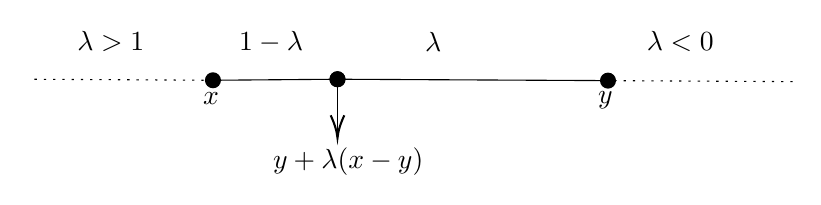
\begin{tikzpicture}[x=0.75pt,y=0.75pt,yscale=-1,xscale=1]
%uncomment if require: \path (0,300); %set diagram left start at 0, and has height of 300

%Straight Lines [id:da13368339552233044] 
\draw    (100,110) -- (160,109.5) ;
\draw [shift={(160,109.5)}, rotate = 359.52] [color={rgb, 255:red, 0; green, 0; blue, 0 }  ][fill={rgb, 255:red, 0; green, 0; blue, 0 }  ][line width=0.75]      (0, 0) circle [x radius= 3.35, y radius= 3.35]   ;
\draw [shift={(100,110)}, rotate = 359.52] [color={rgb, 255:red, 0; green, 0; blue, 0 }  ][fill={rgb, 255:red, 0; green, 0; blue, 0 }  ][line width=0.75]      (0, 0) circle [x radius= 3.35, y radius= 3.35]   ;
%Straight Lines [id:da21549014047251047] 
\draw    (160,109.5) -- (290.33,110.17) ;
\draw [shift={(290.33,110.17)}, rotate = 0.29] [color={rgb, 255:red, 0; green, 0; blue, 0 }  ][fill={rgb, 255:red, 0; green, 0; blue, 0 }  ][line width=0.75]      (0, 0) circle [x radius= 3.35, y radius= 3.35]   ;
\draw [shift={(160,109.5)}, rotate = 0.29] [color={rgb, 255:red, 0; green, 0; blue, 0 }  ][fill={rgb, 255:red, 0; green, 0; blue, 0 }  ][line width=0.75]      (0, 0) circle [x radius= 3.35, y radius= 3.35]   ;
%Straight Lines [id:da8521293809832082] 
\draw    (160,109.5) -- (160,135.83) ;
\draw [shift={(160,137.83)}, rotate = 270] [color={rgb, 255:red, 0; green, 0; blue, 0 }  ][line width=0.75]    (10.93,-3.29) .. controls (6.95,-1.4) and (3.31,-0.3) .. (0,0) .. controls (3.31,0.3) and (6.95,1.4) .. (10.93,3.29)   ;
%Straight Lines [id:da7321314552509732] 
\draw  [dash pattern={on 0.84pt off 2.51pt}]  (100,110) -- (11,109.5) ;
%Straight Lines [id:da2921090265365218] 
\draw  [dash pattern={on 0.84pt off 2.51pt}]  (379.33,110.67) -- (290.33,110.17) ;

% Text Node
\draw (111.33,85.07) node [anchor=north west][inner sep=0.75pt]    {$1-\lambda $};
% Text Node
\draw (201,85.73) node [anchor=north west][inner sep=0.75pt]    {$\lambda $};
% Text Node
\draw (127.67,141.07) node [anchor=north west][inner sep=0.75pt]    {$y+\lambda ( x-y)$};
% Text Node
\draw (94,114.73) node [anchor=north west][inner sep=0.75pt]    {$x$};
% Text Node
\draw (284.33,114.4) node [anchor=north west][inner sep=0.75pt]    {$y$};
% Text Node
\draw (33.4,84.93) node [anchor=north west][inner sep=0.75pt]    {$\lambda  >1$};
% Text Node
\draw (307.8,84.93) node [anchor=north west][inner sep=0.75pt]    {$\lambda < 0$};


\end{tikzpicture}


\caption{Visualization of Convex Combination and Affine Combination, $\lambda x +(1-\lambda)y$.}\label{fig:conx_com}
\end{figure}
\begin{exma}{\bfs{explanation}}
See \cref{fig:conx_com} for details, where please note $\lambda x +(1-\lambda)y = y+\lambda(x-y)$. When $\lambda\in \mathbf{R}$, it is called the \tb{affine (linear) combination}. See \cref{sec:affine} for more details.
\end{exma}
\begin{rema}{\bfs{trivial examples}}
\begin{itemize}
    \item  empty set
    \item singleton (set with single point)
    \item entire space  $\mathbf{R}^{n}$
\end{itemize}
\end{rema}

\begin{exma}{\bfs{polyhedral}}\label{exm:polyh}
The solution set of an \tb{arbitrary (possibly, infinite)} system
of linear inequalities with $n$ unknowns $x$:
\begin{align}
M=\left\{x \in \mathbf{R}^{n} \mid a_{\alpha}^{\top} x \leq b_{\alpha}, \alpha \in \mathcal{A}\right\}\label{eq:gen_ineq}
\end{align}
is convex. In particular, the solution set of a \tb{finite} system
\begin{align*}
A x \preceq b
\end{align*}
of $m$ inequalities with $n$ variables ( $A$ is $m \times n$ matrix) is convex; a set of this latter type is called \tb{polyhedral (polyhedron)}.

Hint: let $x, y$ be two solutions, and let $z=\lambda x+(1-\lambda) y$. For every $\alpha \in \mathcal{A}$ we have
\begin{align*}
\begin{aligned}
&a_{\alpha}^{\top} x \leq b_{\alpha} \\
&a_{\alpha}^{\top} y \leq b_{\alpha}
\end{aligned}
\end{align*}
whence, multiplying the inequalities by \tb{nonnegative} reals $\lambda$ and $1-\lambda$ and taking sum, we have
\begin{align*}
a_{\alpha}^{\top} z=\lambda a_{\alpha}^{\top} x+(1-\lambda) a_{\alpha}^{\top} y \leq \lambda b_{\alpha}+(1-\lambda) b_{\alpha}=b_{\alpha},
\end{align*}
\end{exma}
\begin{exma}\label{exma:plane}What is a plane?
\begin{itemize}
    \item Any \tb{plane} in $\mathbf{R}^{n}$ (in particular, any linear subspace) is the set of all solutions to some system of linear \tb{equations}.
    \item ``A system of linear equations = a system of linear inequalities (a pair of opposite linear inequalities)''$\Rightarrow$  \tb{a plane is a polyhedral set (and convex).}
\end{itemize}
\end{exma}
\begin{exma}{\bfs{nonnegative orthant}}\label{exma:orthnat}
The nonnegative orthant is the set of points with nonnegative components, i.e.,
\begin{align*}
\mathbf{R}_{+}^{n}\coloneqq\left\{x \in \mathbf{R}^{n} \mid x_{i} \geq 0, i=1, \ldots, n\right\}=\left\{x \in \mathbf{R}^{n} \mid x \succeq 0\right\}
\end{align*}
The nonnegative orthant is a polyhedron and a cone (and therefore called a polyhedral cone).
\end{exma}

\begin{defa}{\bfs{Convex Combination}}\label{def:con_com}
 A convex combination of \tb{finitely many} vectors $y_{1}, \ldots, y_{m}$ is their linear combination
\begin{align*}
y=\sum_{i=1}^{m} \lambda_{i} y_{i}, \lambda_{i} \geq 0 \text{ and } \sum_{i=1}^{m} \lambda_{i}=1
\end{align*}
with \tb{nonnegative} coefficients with unit sum.
\end{defa}
\begin{rema}{\bfs{generalize to infinite sums}}\label{rema:gene_con_com}
The idea of a convex combination can be generalized to include \tb{infinite sums, integrals, and, in the most general form, probability distributions}. Suppose $\lambda_{1}, \lambda_{2}, \ldots$ satisfy
\begin{align*}
\lambda_{i} \geq 0, \quad i=1,2, \ldots, \quad \sum_{i=1}^{\infty} \lambda_{i}=1
\end{align*}
and $x_{1}, x_{2}, \ldots \in C$, where $C \subseteq \mathbf{R}^{n}$ is \tb{convex}. Then
\begin{align}
\sum_{i=1}^{\infty} \lambda_{i} x_{i} \in C \label{eq:inf_suma}
\end{align}
if the series converges. More generally, suppose $p: \mathbf{R}^{n} \rightarrow \mathbf{R}$ satisfies $p(x) \geq 0$ for all $x \in C$ and $\int_{C} p(x) d x=1$, where $C \subseteq \mathbf{R}^{n}$ is convex. Then
\begin{align*}
\int_{C} p(x) x d x \in C
\end{align*}
if the integral exists. In the most general form, suppose $C \subseteq \mathbf{R}^{n}$ is convex and $X$ is a random vector with $X \in C$ with probability one. Then $\E X \in C$. Indeed, this form includes all the others as special cases. For example, suppose  $\P\left(X=x_{1}\right)=\theta$ and $\P\left(X=x_{2}\right)=1-\theta$, where $0 \leq \theta \leq 1$. Then $\E X=\theta x_{1}+(1-\theta) x_{2}$, and we are back to a simple convex combination of two points.

Hint: we just need to prove the infinite sums case \cref{eq:inf_suma} since the general case can be then gotten from the DCT. I postpone the proof in \cref{cora:gene_con_com}.
\end{rema}

\begin{lema}{\bfs{equivalence of convex set and convex combination}}\label{eq:equ_conv}
$M$ is convex $\Longleftrightarrow$ any convex combination of vectors from $M$ again is a vector from $M$
\end{lema} 
\begin{rema}
convex set need the line segments between \tb{two} points while convex combination is general \tb{finite} summation.
\end{rema}
\begin{proof}\color{ForestGreen}
"$\Leftarrow$" : assume that $M$ contains all convex combinations of the elements of $M$. Then, with any two points $x, y \in M$ and any $\lambda \in[0,1], M$ contains also the vector $\lambda x+(1-\lambda) y$ since it is a convex combination of $x$ and $y$; thus, $M$ is convex. 

"$\Rightarrow$": assume that $M$ is convex; we should prove that then $M$ contains any convex combination
\begin{align}
y=\sum_{i=1}^{m} \lambda_{i} y_{i}\label{eq:temppr}
\end{align}
of vectors $y_{i} \in M$. The proof is given by \tb{induction} in $m$. 
\begin{enumerate}
    \item The case of $m=1,2$ is evident. Assume that we already know that any convex combination of $m-1$ vectors, $m \geq 3$, from $M$ is again a vector from $M$.
    \item Now prove the case for all convex combinations of $m$ vectors from $M$. Let $y$ be the combination in \cref{eq:temppr}. We can assume that $1>\lambda_{m}$, since otherwise it is obviously correct. Assuming $\lambda_{m}<1$, we can write
\begin{align*}
y=\left(1-\lambda_{m}\right)\left[\sum_{i=1}^{m-1} \frac{\lambda_{i}}{1-\lambda_{m}} y_{i}\right]+\lambda_{m} y_{m}
\end{align*}
What is in the brackets, clearly is a convex combination of $m-1$ points from $M$ and therefore, by the inductive hypothesis, this is a point, let it be called $z$, from $M$; we have
\begin{align*}
y=\left(1-\lambda_{m}\right) z+\lambda_{m} y_{m}
\end{align*}
with $z$ and $y_{m} \in M$, and $y \in M$ by definition of a convex set $M$.
\end{enumerate}  
\end{proof} 
\begin{lema}{\bfs{convexity of intersections}}\label{lem:con_inter} Let $\left\{M_{\alpha}\right\}_{\alpha}$ be an arbitrary family of convex subsets of $\mathbf{R}^{n}$. Then the intersection
\begin{align*}
M=\cap_{\alpha} M_{\alpha}
\end{align*}
is convex.
\begin{proof}\color{ForestGreen}
easy
\end{proof}
\end{lema}
\begin{defa}{\bfs{Convex Hull}} 
 $\operatorname{Conv}(M)$  is the \tb{smallest} convex set containing $M$, namely, the \tb{intersection of all convex sets containing $M$}.
\end{defa}
\begin{rema}
If $M$ is convex, $\operatorname{Conv}(M)=M$.
\end{rema}
\begin{cora}{\bfs{convex hull via convex combinations}}\label{eq:con_conx_com}
For a nonempty $M \subset \mathbf{R}^{n}$ :
$$\operatorname{Conv}(M)=M^{*}\coloneqq\{ \text{the set of all convex combinations of vectors from } M\} $$
\end{cora}
\begin{proof}\color{ForestGreen}
According to \cref{eq:equ_conv}, $M^{*}\subset \operatorname{Conv}(M)$ since $\operatorname{Conv}(M)$ is a convex set containg $M$. We need show $\operatorname{Conv}(M)\subset M^{*}$. We need to prove  $M^{*}$ is convex. To prove that $M^{*}$ is convex is the same as to prove that any convex combination $\nu x+(1-\nu) y$ of any two points $x=\sum_{i} \lambda_{i} x_{i}, y=\sum_{i} \mu_{i} x_{i}$ of $M^{*}$ (if two different set $\{x_i\}$, just use the union) is again a convex combination of vectors from $M$. This is evident:
\begin{align*}
\nu x+(1-\nu) y=\nu \sum_{i} \lambda_{i} x_{i}+(1-\nu) \sum_{i} \mu_{i} x_{i}=\sum_{i} \xi_{i} x_{i}, \quad \xi_{i}=\nu \lambda_{i}+(1-\nu) \mu_{i}
\end{align*}
and the coefficients $\xi_{i}$ clearly are nonnegative with unit sum. 
\end{proof}



\begin{rema}{\bfs{two descriptions of convex set}}\label{rema:two_des}
\begin{itemize}
    \item \tb{inner (``worker's'')} description: convex combination (hull) of all points (see\cref{def:con_com})
    \item \tb{outer (``artist's'')} description for \tb{closed} convex set: 
 In \cref{eq:gen_ineq}, we show that \tb{the  intersection of closed half-spaces is closed convex}. The converse is also true:  For every $x \notin M$, we can find the closed half-space $H_{x}=\left\{y \mid a_{x}^{\top} y \leq \alpha_{x}\right\}$ which contains $M$ and does not contain $x$; consequently.
\begin{align*}
M=\bigcap_{x \notin M} H_{x}
\end{align*}
and therefore \tb{$M$ equals intersection of all closed half-spaces which contain $M$.} (see \cref{sec:out_conx}. note it is solution set to nonstrict linear (possibly, infinite many) inequalities  \cref{eq:gen_ineq})
\end{itemize}
\end{rema}









\subsubsection{Affine}\label{sec:affine}
\begin{defa}{\bfs{Affine Set and Lines}}
 \begin{enumerate}
     \item Let $x, y$ be two points in $\mathbf{R}^{n}$. The set
\begin{align*}
\{z=\lambda x+(1-\lambda) y \mid \lambda \in\mathbf{R}\}
\end{align*}
is called a \tb{line} going through $x, y .$
\item A subset $M$ of $\mathbf{R}^{n}$ is called \tb{affine}, if $\forall x, y\in M$, $M$ contains the line going through $x, y $:
\begin{align*}
\forall x, y \in M, \lambda \in \mathbf{R}, \lambda x+(1-\lambda) y \in M.
\end{align*}
 \end{enumerate}
\end{defa}

\begin{defa}{\bfs{Affine Combination}}\label{def:aff_com}
 A convex combination of \tb{finitely many} vectors $y_{1}, \ldots, y_{m}$ is their linear combination
\begin{align*}
y=\sum_{i=1}^{m} \lambda_{i} y_{i}, \lambda_{i} \in \mathbf{R} \text{ and } \sum_{i=1}^{m} \lambda_{i}=1
\end{align*}
with  coefficients with unit sum.
\end{defa}

\begin{defa}{\bfs{Affine Hull}}
 $\Aff(M)$ the smallest affine set containing $M$, namely, the intersection of all affine sets containing $M$. 
\end{defa}
\begin{rema}
Intuitively,  $\Aff(M)$ is the "proper" space to look at $M:$ we simply cut from $\mathbf{R}^{n}$ "useless" dimensions (such that the projection of $M$ on these dimensions is a singleton.
\end{rema}

\begin{cora}{\bfs{affine hull via affine combinations}}
For a nonempty $M \subset \mathbf{R}^{n}$ :
$$\operatorname{Aff}(M)=\{ \text{the set of all affine combinations of vectors from } M\} $$
\end{cora}
\begin{proof}\color{ForestGreen}
Similar to the proof to \cref{eq:con_conx_com}.
\end{proof}
\begin{rema}{\bfs{Convex vs. Affine}} From the definitions, we have 
$$\text{affine } \Rightarrow \text{ convex}$$
See also \cref{rema:con_aff_cone} for more comparison.
\end{rema}

\paragraph{Affine Set = Subspace + Translate}
If $C$ is an affine set and $x_{0} \in C$, then the set
\begin{align*}
V=C-x_{0}=\left\{x-x_{0} \mid x \in C\right\}
\end{align*}
is a subspace, i.e., closed under sums and scalar multiplication. To see this, suppose $v_{1}, v_{2} \in V$ and $\alpha, \beta \in \mathbf{R}$. Then we have $v_{1}+x_{0} \in C$ and $v_{2}+x_{0} \in C$, and so
\begin{align*}
\alpha v_{1}+\beta v_{2}+x_{0}=\alpha\left(v_{1}+x_{0}\right)+\beta\left(v_{2}+x_{0}\right)+(1-\alpha-\beta) x_{0} \in C
\end{align*}
since $C$ is affine, and $\alpha+\beta+(1-\alpha-\beta)=1 .$ We conclude that $\alpha v_{1}+\beta v_{2} \in V$.

\begin{lema}
Thus, the affine set $C$ can be expressed as:
\begin{align*}
C=V+x_{0}=\left\{v+x_{0} \mid v \in V\right\},
\end{align*}
which is also called the \tb{translate of the subspace $V$}.
\end{lema}
\begin{rema}
The subspace $V$ associated with the affine set $C$ does not depend on the choice of $x_{0}$, so $x_{0}$ can be chosen as any point in $C$.
\end{rema}
\begin{defa}{\bfs{Affine Dimension}}
  We define the dimension of an affine set $C$ as the dimension of the subspace $V=C-x_{0}$, where $x_{0}$ is any element of $C$.
\end{defa}


\begin{exma}{\bfs{solution set of linear equations}}\label{exm:linear_aff}
  The solution set of a system of linear equations, $C=\{x \mid A x=b\}$, where $A \in \mathbf{R}^{m \times n}$ and $b \in \mathbf{R}^{m}$, is an \tb{affine set}. To show this, suppose $x_{1}, x_{2} \in C$, i.e., $A x_{1}=b, A x_{2}=b$. Then for any $\theta$, we have
\begin{align*}
\begin{aligned}
A\left(\theta x_{1}+(1-\theta) x_{2}\right) &=\theta A x_{1}+(1-\theta) A x_{2} \\
&=\theta b+(1-\theta) b \\
&=b
\end{aligned}
\end{align*}
which shows that the affine combination $\theta x_{1}+(1-\theta) x_{2}$ is also in $C$. \tb{The subspace associated with the affine set $C$ is the nullspace of $A$.}

We also have a \tb{converse: every affine set can be expressed as the solution set of a system of linear equations.} This is because every affine set can be expressed as translate to a subspace, and every subspace could be expressed as the null space of a linear mapping. One choice for the linear mapping is the projection as shown in \cite[229]{rudin1976principles}.
\tb{$$\text{affine set}\Longleftrightarrow \text{solution set of  a system of linear equations}$$}
\end{exma}

\paragraph{Affine Independent}
\begin{defa}{\bfs{Affine Independent}}\label{sec:aff_ind}
 Let $v_{0}, v_{1} \ldots v_{k}$ be points in $\mathbf{R}^{n}$. These points are called \tb{affinely independent} if ``$\sum_{i=0}^{k} \lambda_{i} v_{i}=0$ and $\sum_{i=0}^{k} \lambda_{i}=0$ $\Rightarrow \lambda_{i}=0, \forall i$''
\end{defa} 

\begin{lema}{\bfs{Affine Independent and Linear Independent}}

\centerline{ ``$v_{0}, v_{1} \ldots v_{k}$ are affinely independent'' $\Longleftrightarrow$ ``$v_{1}-v_{0}, v_{2}-v_{0} \ldots v_{k}-v_{0}$ are linearly independent''}
\end{lema}
\begin{rema}
$v_{0}$ can be replaced by any $v_{i}$, which is called a \tb{base point}.
\end{rema}
\begin{proof}\color{ForestGreen}
``$\Rightarrow$'': Consider some $\lambda_{1}, \ldots, \lambda_{k}$, such that:
\begin{align*}
\sum_{i=1}^{k} \lambda_{i}\left(v_{i}-v_{0}\right)=0
\end{align*}
Consider some $\lambda_{0} \in \mathbf{R}$, such that $\sum_{i=0}^{k} \lambda_{i}=0$
Also, we have:
\begin{align*}
\sum_{i=0}^{k} \lambda_{i} v_{i}=\sum_{i=1}^{k} \lambda_{i}\left(v_{i}-v_{0}\right)+\left(\sum_{i=0}^{k} \lambda_{i}\right) v_{0} = 0
\end{align*}
We get $\lambda_{i}=0, \forall i$ due to affine independence, i.e. $v_{i}-v_{0}$ are linear independent.

``$\Leftarrow$'': Consider some $\lambda_{0}, \lambda_{1}, \ldots, \lambda_{k}$, such that: $\sum_{i=0}^{k} \lambda_{i} v_{i}=0$ and $\sum_{i=0}^{k} \lambda_{k}=0$
We have to show that all these coefficients must be zero under the condition of linear independence. We have $\sum_{i=1}^{k} \lambda_{i}\left(v_{i}-v_{0}\right)=0$. Therefore, due to linear independence of $\left(v_{i}-v_{0}\right)$, we conclude that:
\begin{align*}
\lambda_{1}=\lambda_{2}=\ldots=\lambda_{k}=0
\end{align*}
Also, $\sum_{i=0}^{k} \lambda_{k}=0 \Rightarrow \lambda_{0}=0$
This proves that they are affinely independent.
\end{proof}






\subsubsection{Cone}
\begin{defa}{\bfs{Conic}}
 A nonempty subset $M$ of $\mathbf{R}^{n}$ is called \tb{conic}, if it contains, along with every point $x \in M$, the entire ray $\mathbf{R}_x=\{t x \mid t \geq 0\}$ spanned by the point:
\begin{align*}
\forall x \in M , t\ge 0,  tx \in M
\end{align*}
\end{defa}
\begin{defa}{\bfs{Cone}}
 A \tb{convex conic} set is called a \tb{cone}\footnote{In \cite{boyd2004convex}, conic is called cone, while cone is called convex cone}. Analogy to \cref{def:con_seg}, we have: A subset $M$ of $\mathbf{R}^{n}$ is called \tb{cone}, if $\forall x, y\in M$, $M$ contains all conic combinations (see below for definition) of $x,y$:
\begin{align*}
\forall x, y \in M, \lambda_1,\lambda_2\ge 0, \lambda_1 x+\lambda_2 y \in M.
\end{align*}
\end{defa}
\begin{rema}
See \cref{fig:cone} for \tb{conic} example. 
Note $\lambda_1 x+\lambda_2 y =\alpha(\beta x+(1-\beta)y)$ for some $\alpha,\beta\ge 0$. So it contains the rays going through any convex combination of $x$ and $y$. The convex combination could be relaxed to sum (see \cref{rema:equ_coni}). 
\end{rema}
\begin{figure}
    \centering
    \includegraphics[width=0.5\textwidth]{Figs/cone-min.png}
    \caption{Conic}
    \label{fig:cone}
\end{figure}
\begin{rema}{\bfs{Convex vs. Affine vs. Cone}}\label{rema:con_aff_cone} 
\begin{itemize}
    \item convex: $\lambda_i\ge 0$ and $\sum_i\lambda_i=1$.
    \item affine: $\sum_i\lambda_i=1$.
    \item cone: $\lambda_i\ge 0, \forall i$ ($\lambda \succeq 0$) 
    \item so we have affine $\Rightarrow$ convex, and cone $\Rightarrow$ convex.
\end{itemize}
\end{rema}
\begin{defa}{\bfs{Conic Combination}}\label{def:cone_com}
 A conic combination of \tb{finitely many} vectors $y_{1}, \ldots, y_{m}$ is their linear combination
\begin{align*}
y=\sum_{i=1}^{m} \lambda_{i} y_{i}, \lambda_{i} \geq 0 
\end{align*}
with \tb{nonnegative} coefficients.
\end{defa}
\begin{defa}{\bfs{Conic Hull}} 
 $\operatorname{Conic}(M)$  is the \tb{smallest} cone set containing $M$, namely, the \tb{intersection of all cone sets containing $M$}. This is because the intersection of cones is still a cone (analogous to \cref{lem:con_inter})
\end{defa}
\begin{cora}{\bfs{conic hull via conic combinations}}
For a nonempty $M \subset \mathbf{R}^{n}$ :
$$\operatorname{Cone}(M)=\{ \text{the set of all conic combinations of vectors from } M\} $$
\end{cora}
\begin{proof}\color{ForestGreen}
Similar to the proof to \cref{eq:con_conx_com}.
\end{proof}

\begin{rema}{\bfs{equivalent statement}}\label{rema:equ_coni}
A nonempty subset $M$ of $\mathbf{R}^{n}$ is a cone if and only if it possesses the following pair of properties:
\begin{itemize}
    \item is conic: $\forall x \in M, t \geq 0, t x \in M$;
    \item contains sums of its elements: $\forall x, y \in M, x+y \in M$.
\end{itemize}
\end{rema}

\paragraph{Polyhedral Cone: inner and outer description}
\begin{exma}\label{exma:ply_con}
 The solution set of an arbitrary (possibly, infinite) system, $a_{\alpha}^{\top} x \leq 0, \alpha \in \mathcal{A}$, 
of \tb{homogeneous linear inequalities} with $n$ unknowns $x$, namely, the set
\begin{align*}
K=\left\{x \mid a_{\alpha}^{\top} x \leq 0, \forall \alpha \in \mathcal{A}\right\}
\end{align*}
is a \tb{cone}. In particular, the solution set to a homogeneous \tb{finite} system of $m$ homogeneous linear inequalities
\begin{align*}
A x \preceq 0
\end{align*}
( $A$ is $m \times n$ matrix $)$ is a cone; a cone of this latter type is also a {polyhedral} as mentioned in \cref{exm:polyh}, we call it the \tb{polyhedral cone} 
\end{exma}
\begin{rema}\label{rema:homo_con}
Compare with \cref{exm:polyh}, $0$ on the right hand side is very important. Only $0$ guarantees the cone. $ab\le b, \forall a\ge 0\Rightarrow a=0$.  
\end{rema}

\begin{rema}\label{rema:cone_outer} Note that the cones given by systems of linear homogeneous nonstrict inequalities necessarily are closed.
Similar to \cref{exm:linear_aff} and \cref{rema:two_des}, we have 
\tb{$$\text{closed cone}\Longleftrightarrow \text{solution set for linear homogeneous nonstrict inequalities}$$}
This is because closed cone are convex and thus could be expressed using the closed half-spaces in \cref{rema:two_des}. Since it is a conic, we then have the half-spaces $\left\{y \mid a_{x}^{\top} y \leq \alpha_{x}\right\}$ need to be \tb{homogeneous linear inequalities} (i.e. with $\alpha_{x}=0$, similar to the reason mentioned in \cref{rema:homo_con})

We therefore have the special case of the \tb{outer description of closed convex cone} (for the general case of closed convex set see \cref{sec:out_conx}):

\tb{\centerline{a closed cone is the intersection of all homogeneous halfspaces containing the cone.}}

\end{rema}

\begin{exma}
 In particular, the conic hull of a nonempty \tb{finite} set $M=\left\{u_{1}, \ldots, u_{N}\right\}$ of vectors in $\mathbf{R}^{n}$ is the cone
\begin{align*}
\operatorname{Cone}(M)=\left\{\sum_{i=1}^{N} \lambda_{i} u_{i} \mid \lambda_{i} \geq 0, i=1, \ldots, N\right\}
\end{align*}
\end{exma}
\begin{rema}
This is the \tb{inner} description of a polyhedral cone while the set given by finitely many homogeneous linear inequalities in \cref{exma:ply_con} is \tb{outer} description.
\end{rema}
\begin{lema}{\bfs{Weyl-Minkowski Lemma}}

\tb{``inner description with finite vectors'' $\Leftrightarrow$ ``outer with finite homogeneous linear inequalities''}
\end{lema}
\begin{proof}\color{ForestGreen}
Let $K$ be a finitely generated cone. Then for some matrix $D$ we have
\begin{align*}
\begin{aligned}
K &=\left\{x \in \mathbf{R}^{n}: x=D y \text { for some } y \succeq 0\right\} \\
&=\left\{x \in \mathbf{R}^{n}: \text { the system } x-D y=0, y \succeq 0 \text { is consistent in } x, y\right\} \\
&=\left\{x \in \mathbf{R}^{n}: B x \succeq 0\right\} \quad \text { for some matrix } B\\
&=\left\{x \in \mathbf{R}^{n}: -B x \preceq 0\right\} \quad \text { for some matrix } B
\end{aligned}
\end{align*}
by using Fourier-Motzkin elimination to eliminate $y$.
\end{proof}


\paragraph{Homogeneous Farkas Lemma}

\begin{thma}{\bfs{Homogeneous Farkas Lemma}}\label{thm:Farkas}
Let ${A} \in \mathbf{R}^{n \times N}$ and ${b} \in \mathbf{R}^{n}$. Then exactly one of the following two assertions is true:
\begin{enumerate}
    \item There exists an ${\lambda} \in \mathbf{R}^{N}$ such that ${A} {\lambda}={b}$ and ${\lambda} \succeq 0$
    \item There exists a ${h} \in \mathbf{R}^{n}$ such that ${A}^{\top} {h} \succeq  0$ and ${b}^{\top} {h}<0$.
\end{enumerate}
\end{thma} 
\begin{rema}{\bfs{explanation}}
$n$: vector dimension; $N$: number of vectors. Consider the closed convex cone $C(A)$ spanned by the columns of $A$; that is,
\begin{align*}
C(A)=\{A \lambda \mid {\lambda}\succeq 0\}
\end{align*}
Observe that $C(A)$ is the set of the vectors $b$ for which the first assertion in the statement of Farkas' lemma holds. On the other hand, the vector \tb{$h$ in the second assertion is orthogonal to a hyperplane that separates $b$ and $C(A)$}. 

The lemma follows from the observation that $b$ belongs  to ${ C(A )}$ if and only if there is no hyperplane that separates it from ${ C(A )}$.
More precisely, let $a_{1}, \ldots,a_{N} \in \mathbf{R}^{n}$ denote the columns of $A$. In terms of these vectors, Farkas' lemma states that exactly one of the following two statements is true:
\begin{enumerate}
    \item  There exist \tb{nonnegative} coefficients $\lambda_{1}, \ldots, \lambda_{N}\in \mathbf{R}$ such that $b=\lambda_{1}a_{1}+\cdots+\lambda_{n}a_{N}$
    \item There exists a vector $h \in \mathbf{R}^{n}$ such that $a_{i}^{\top} h \geq {0}$ for $i=1, \ldots, N$, and $b^{\top} h<0$.
\end{enumerate}
\end{rema}
\begin{proof}\color{ForestGreen}
We need to prove if $b\notin C(A)$, we have 2). From the separation of a convex set and a point outside of the set in \cref{lem:sep_con_pointnotin}, we know there exists a hyperplane that strongly separate $b$ and $C(A)$, i.e. $$b^{\top} h< \inf_{a\in C(A)} a^{\top}h$$
We only need to show  $$b^{\top} h<0\le \inf_{a\in C(A)} a^{\top}h.$$
Select point $a=\mathbf{0}\in C(A)$, we get $b^{\top} y<0$. If we can select one $a\in C(A)$ s.t. $a^{\top}h=-\epsilon$, where $\epsilon>0$, for a large enough $\alpha$, we have $\alpha a^{\top}h=-\alpha\epsilon<b^{\top} h$, a contradiction. We therefore have $b^{\top} h<0\le \inf_{a\in C(A)} a^{\top}h.$
\end{proof}

\begin{cora}{\bfs{Extended Farkas Lemma: sufficient and necessary}}\label{cora:Farkas}
 Let $b, a_{1}, \ldots, a_{N}$ be vectors from $\mathbf{R}^{n}$. 
 
 \centerline{\tb{``$b$ is a conic combination of  $a_{i}$'' $\Longleftrightarrow$ ``$h$ satisfies that $h^{\top} a_{i} \geq 0, i=1, \ldots, N$ $\Rightarrow$  $h^{\top} b \geq 0 $''}}
 \end{cora}
\begin{proof}\color{ForestGreen}
``$\Rightarrow$'': This is a restatement of \cref{thm:Farkas}. 

``$\Leftarrow$'': Assume that every vector $h$ satisfying $h^{\top} a_{i} \geq 0 \forall i$ satisfies also $h^{\top} b \geq 0$, and we need to prove that $b$ is a conic combination of the vectors $a_{i}$.

From \cref{rema:cone_outer}, we know the set $\Cone(\left\{a_{1}, \ldots, a_{N}\right\})$ of all conic combinations of $a_{1}, \ldots, a_{N}$ is polyhedrally representable:
\begin{align}
\Cone(\left\{a_{1}, \ldots, a_{N}\right\})=\left\{x \mid p_{j}^{\top} x \geq 0, 1 \leq j \leq J\right\}\label{eq:cone_tt}
\end{align}
 For every $j$, relation $p_{j}^{\top} a_{i} \geq 0$ for all $i$ implies, by the premise of the statement we want to prove, that $p_{j}^{\top} b \geq 0$. We see that $p_{j}^{\top} a \geq 0$ for all $j$, meaning that $b$ indeed belongs to the cone \cref{eq:cone_tt}.
\end{proof}
\begin{cora}{\bfs{Generalized Farkas Lemma}}\label{cora:gene_fark}
Let $A \in \mathbf{R}^{n \times N}, b \in \mathbf{R}^{n}, S$ is a closed convex cone in $\mathbf{R}^{N}$, and the dual cone of $S$ is $S^{*}=\left\{z \in \mathbf{R}^{N} \mid z^{\top} \lambda \geq 0, \forall \lambda \in S\right\}$. If convex cone $C(A)=\{{A \lambda} \mid \lambda \in S\}$ is closed, then exactly one of the following two statements is true:
\begin{enumerate}
    \item There exists an $\lambda \in \mathbf{R}^{N}$ such that ${A \lambda}=b$ and $\lambda \in S$
    \item There exists a ${h} \in {R}^{n}$ such that $A^{\top} {h} \in S^{*}$ and $b^{\top} {h}<0$
\end{enumerate}
\end{cora}
\begin{rema}{\bfs{explanation of generalized Farkas' lemma}}
Either a vector is in a given closed convex cone, or there exists a hyperplane separating the vector from the cone; there are no other possibilities.  See also \cref{sec:bmqdfd} for \tb{strong alternatives}.

The closedness condition is necessary. For original Farkas' lemma, $S$ is the nonnegative orthant $\mathbf{R}_{+}^{N}$, hence the closedness condition holds automatically. For polyhedral convex cone, the closedness condition holds automatically from the outer description.
\end{rema}
\begin{rema}{\bfs{solvability  of finite linear equalities}}
By setting $S=\mathbf{R}^{n}$ and $S^{*}=\{0\}$ in generalized Farkas' lemma, we obtain the following corollary about the solvability for a finite system of linear equalities:

 Let $A \in \mathbf{R}^{n \times N}$ and $b \in \mathbf{R}^{N}$. Then exactly one of the following two statements is true:
\begin{enumerate}
    \item There exists an $\lambda \in \mathbf{R}^{N}$ such that ${A \lambda}=b$
    \item There exists a ${h} \in \mathbf{R}^{n}$ such that $A^{\top} {h}={0}$ and $b^{\top} {h} \neq {0}$.  (note here $\ne$ is equivalent to $<$ because of the former  $A^{\top} {h}={0}$)
\end{enumerate}
\end{rema}


\begin{cora}{\bfs{generalized convex combination \cref{rema:gene_con_com}}}\label{cora:gene_con_com}
Suppose $\lambda_{1}, \lambda_{2}, \ldots$ satisfy
\begin{align*}
\lambda_{i} \geq 0, \quad i=1,2, \ldots, \quad \sum_{i=1}^{\infty} \lambda_{i}=1
\end{align*}
and $x_{1}, x_{2}, \ldots \in C$, where $C \subseteq \mathbf{R}^{n}$ is \tb{convex}. Then
\begin{align}
\sum_{i=1}^{\infty} \lambda_{i} x_{i} \in C \label{eq:inf_sum}
\end{align}
if the series converges.
\end{cora}
\begin{proof}\color{ForestGreen}
We can show by \tb{induction on dimension} (the base case $n=0$ being trivial). Let $x=\sum_{i=1}^{\infty} \lambda_{i} x_{i}$, and let
\begin{align}
V\coloneqq\mathbf{R}_{>0}(C-x)=\left\{y \in \mathbf{R}^{n} \mid x+\alpha y \in C \text { for some } \alpha>0\right\}\label{eq:fdafadg}
\end{align}
Since $C$ is convex, $V$ is a convex cone. If $V=\mathbf{R}^{n}$ then $0 \in V$ implies $x \in C$, and we are done. Suppose $V \neq \mathbf{R}^{n}$. From Farkas lemma, $V$ is contained in a half-space
\begin{align*}
H=\left\{y \in \mathbf{R}^{n} \mid h \cdot y \leq 0\right\}
\end{align*}
where $h \in \mathbf{R}^{n}$ is nonzero. Hence $h \cdot c \leq \lambda$ for all $c \in C$ where $\lambda=h \cdot x$ from definition \cref{eq:fdafadg}. In particular
\begin{align*}
\lambda=\sum_{i=1}^{\infty} \lambda_{i}\left(h \cdot x_{i}\right) \leq\left(\sum_{i=1}^{\infty} \lambda_{i}\right) \lambda=\lambda
\end{align*}
so we must have $h \cdot x_{i}=\lambda$ for each $i$ with $\lambda_{i}>0$. Now the result follows from the inductive hypothesis applied to the hyperplane
$\left\{y \in \mathbf{R}^{n} \mid h \cdot y=\lambda\right\}$, which has dimension $n-1$.
\end{proof} 
\subsubsection{Operations Preserve Convexity}

\paragraph{Intersection} It is \cref{lem:con_inter}. Let $\left\{M_{\alpha}\right\}_{\alpha}$ be an arbitrary family of convex subsets of $\mathbf{R}^{n}$. Then the intersection
\begin{align*}
M=\cap_{\alpha} M_{\alpha}
\end{align*}
is convex.
\begin{itemize}[noitemsep,topsep=0pt]
    \item \begin{exma}\vspace{-0.4cm}{\bfs{positive semidefinite cone}}
The positive semidefinite cone $S_{+}^{n}$ can be expressed as
\begin{align*}
\bigcap_{z \neq 0}\left\{X \in S^{n} \mid z^{\top} X z \geq 0\right\} .
\end{align*}
For each $z \neq 0, z^{\top} X z$ is a (not identically zero) linear function of $X$, so the sets
\begin{align*}
\left\{X \in S^{n} \mid z^{\top} X z \geq 0\right\}
\end{align*}
are, in fact, halfspaces in $S^{n}$. Thus the positive semidefinite cone is the intersection of an infinite number of halfspaces, and so is convex.
\end{exma}
\item \begin{exma}\vspace{-0.4cm}
 We consider the set
\begin{align*}
S=\left\{x \in \mathbf{R}^{m}|| p(t) \mid \leq 1 \text { for }|t| \leq \pi / 3\right\}
\end{align*}
where $p(t)=\sum_{k=1}^{m} x_{k} \cos k t$. The set $S$ can be expressed as the intersection of an infinite number of slabs: $S=\bigcap_{|t| \leq \pi / 3} S_{t}$, where
\begin{align*}
S_{t}=\left\{x \mid-1 \leq(\cos t, \ldots, \cos m t)^{\top} x \leq 1\right\}
\end{align*}
and so is convex.
\end{exma}
\end{itemize}

\paragraph{Cartesian Product and Projection} 
\tb{$\bullet$ Cartesian product:}

If $S_{1}$ and $S_{2}$ are convex, then so is the Cartesian product
$$S_{1} \times S_{2}=\left\{\left(x_{1}, x_{2}\right) \mid x_{1} \in S_{1}, x_{2} \in S_{2}\right\}$$

\tb{$\bullet$ Two projection:}
\begin{itemize}
    \item The projection of a convex set onto some of its coordinates is convex: if $S \subseteq \mathbb{R}^{m} \times \mathbb{R}^{n}$ is convex, then
\begin{align*}
T=\left\{x_{1} \in \mathbb{R}^{m} \mid\left(x_{1}, x_{2}\right) \in S \text { for some } x_{2} \in \mathbb{R}^{n}\right\}
\end{align*}
is convex.
\item  If $S \subseteq \mathbb{R}^{m} \times \mathbb{R}^{n}$ is convex, then for any constant $h$,
\begin{align*}
T=\left\{x_{1} \in \mathbb{R}^{m} \mid\left(x_{1}, h\right) \in S\right\}
\end{align*}
is convex or empty.
\end{itemize}



\paragraph{Affine Mapping}

\tb{1). image under affine mapping:}

If $M \subset \mathbf{R}^{n}$ is convex and $x \mapsto \mathcal{A}(x) \equiv A x+b$ is an affine mapping from $\mathbf{R}^{n}$ into $\mathbf{R}^{m}$ ($A$ is $m \times n$ matrix, $b$ is $m$-dimensional vector), then the set
\begin{align*}
\mathcal{A}(M)=\{y=\mathcal{A}(x) \equiv A x+b \mid x \in M\}
\end{align*}
is a convex set in $\mathbf{R}^{m}$.


\tb{2). inverse image under affine mapping: }

If $M \subset \mathbf{R}^{n}$ is convex and $y \mapsto A y+b$ is an affine mapping from $\mathbf{R}^{m}$ to $\mathbf{R}^{n}$ (A is $n \times m$ matrix, $b$ is $n$-dimensional vector), then the set
\begin{align*}
\mathcal{A}^{-1}(M)=\left\{y \in \mathbf{R}^{m} \mid \mathcal{A}(y) \in M\right\}
\end{align*}
is a convex set in $\mathbf{R}^{m}$.

\begin{itemize}
    \item \begin{exma}\vspace{-0.5cm}{\bfs{polyhedron}}
 The polyhedron $\{x \mid A x \preceq b, C x=d\}$ ($C x=d$ can be ignored, same as in \cref{exm:polyh}. see \cref{exma:plane}) can be expressed as the inverse image of the Cartesian product of the nonnegative orthant (\cref{exma:orthnat}) and the origin under the affine function $f(x)=(b-A x, d-C x)$ :
\begin{align*}
\{x \mid A x \preceq b, C x=d\}=\left\{x \mid f(x) \in \mathbf{R}_{+}^{m} \times\{0\}\right\}
\end{align*}
\end{exma}
\item \begin{exma}\vspace{-0.5cm}{\bfs{solution set of linear matrix inequality}}  The condition
\begin{align*}
A(x)=x_{1} A_{1}+\cdots+x_{N}A_{n} \preceq B
\end{align*}
where $B, A_{i} \in S^{m}$, is called a linear matrix inequality $(\mathrm{LMI})$ in $x .$ (Note the similarity to an ordinary linear inequality,
\begin{align*}
a^{\top} x=x_{1} a_{1}+\cdots+x_{N}a_{N} \leq b
\end{align*}
with $b, a_{i} \in \mathbf{R} .$)
The solution set of a linear matrix inequality, $\{x \mid A(x) \preceq B\}$, is convex. Indeed, it is the inverse image of the positive semidefinite cone under the affine function $f: \mathbf{R}^{n} \rightarrow S^{m}$ given by $f(x)=B-A(x)$
\end{exma}
\end{itemize}

\paragraph{Arithmetic Summation and Multiplication by Reals:} If $M_{1}, \ldots, M_{k}$ are convex sets in $\mathbf{R}^{n}$ and $\lambda_{1}, \ldots, \lambda_{k}$ are \tb{arbitrary reals (no need $\ge 0$)}, then the set
\begin{align*}
\lambda_{1} M_{1}+\ldots+\lambda_{k} M_{k}=\left\{\sum_{i=1}^{k} \lambda_{i} x_{i} \mid x_{i} \in M_{i}, i=1, \ldots, k\right\}
\end{align*}
is convex.
\begin{rema}
We can take this as the affine mapping from $M_{1}\times \ldots\times M_{k}\rightarrow \mathbf{R}$, so the conclusion holds.
\end{rema}

\paragraph{Linear-fractional and Perspective Function} 

\tb{1). image under perspective function:}
\begin{defa}{\bfs{Perspective Function}}
 \begin{align*}
    P: \mathbf{R}^{n} \times \mathbf{R}_{++} &\rightarrow \mathbf{R}^{n}\\ 
        (z, t)&\mapsto z / t
\end{align*}
\end{defa}

Suppose that $x=\left(\tilde{x}, x_{n+1}\right), y=\left(\tilde{y}, y_{n+1}\right) \in \mathbf{R}^{n+1}$ with $x_{n+1}>0$, $y_{n+1}>0 .$ Then for $0 \leq \theta \leq 1$
\begin{align*}
P(\theta x+(1-\theta) y)=\frac{\theta \tilde{x}+(1-\theta) \tilde{y}}{\theta x_{n+1}+(1-\theta) y_{n+1}}=\mu P(x)+(1-\mu) P(y)
\end{align*}
where
\begin{align*}
\mu=\frac{\theta x_{n+1}}{\theta x_{n+1}+(1-\theta) y_{n+1}} \in[0,1] .
\end{align*}
As $\theta$ varies between 0 and 1 (which sweeps out the line segment $[x, y]), \mu$ varies between 0 and 1 (which sweeps out the line segment $[P(x), P(y)])$. This shows that $P([x, y])=[P(x), P(y)]$. We therefore get 
\begin{align}
   \text{\tb{$P(C)$ is convex if $C \subseteq \dom  P$ is convex}} \label{eq:ps}
\end{align}

\begin{rema}
  Geometrically, with each point $z$ in $\mathbf{R}^{n}$ we associate the (open) ray $\mathcal{P}(z)=\{t(z, 1) \mid t>0\}$ in $\mathbf{R}^{n+1} .$ That means we get 
  
  \tb{\centerline{1-1 matching between $\mathbf{R}^{n}$ and a set of rays in $\mathbf{R}^{n+1}$}}
\end{rema}

\tb{2). inverse image under perspective function:}

If $C \subseteq \mathbf{R}^{n}$ is convex, then
\begin{align*}
P^{-1}(C)=\left\{(x, t) \in \mathbf{R}^{n+1} \mid x / t \in C, t>0\right\}
\end{align*}
is convex. To show this, suppose $(x, t) \in P^{-1}(C),(y, s) \in P^{-1}(C)$, and $0 \leq \theta \leq 1$. We need to show that
\begin{align*}
\theta(x, t)+(1-\theta)(y, s) \in P^{-1}(C)
\end{align*}
i.e., that
\begin{align*}
\frac{\theta x+(1-\theta) y}{\theta t+(1-\theta) s} \in C
\end{align*}
This follows from
\begin{align*}
\frac{\theta x+(1-\theta) y}{\theta t+(1-\theta) s}=\mu\frac{x}{t}+(1-\mu)\frac{y}{s}
\end{align*}
where
\begin{align*}
\mu=\frac{\theta t}{\theta t+(1-\theta) s} \in[0,1] .
\end{align*}
We therefore have 
\begin{align}
   \text{\tb{$P^{-1}(C)$ is convex if $C \subseteq$ is convex}}\label{eq:ps_inv}
   \end{align}

\tb{3) image and inverse image under linear-fractional functions:}

A linear-fractional function is formed by composing the perspective function with an affine function. Suppose $g: \mathbf{R}^{n} \rightarrow \mathbf{R}^{m+1}$ is affine, i.e.,
\begin{align*}
g(x)=\left[\begin{array}{c}
A \\
c^{\top}
\end{array}\right] x+\left[\begin{array}{l}
b \\
d
\end{array}\right]
\end{align*}
where $A \in \mathbf{R}^{m \times n}, b \in \mathbf{R}^{m}, c \in \mathbf{R}^{n}$, and $d \in \mathbf{R} .$ The function $f: \mathbf{R}^{n} \rightarrow \mathbf{R}^{m}$ given
by $f=P \circ g$, i.e.
\begin{align*}
f(x)=(A x+b) /\left(c^{\top} x+d\right), \quad \dom  f=\left\{x \mid c^{\top} x+d>0\right\}
\end{align*}

\begin{rema}{\bfs{affine, linear vs. linear-fractional}}
If $c=0$ and $d>0$, the domain
of $f$ is $\mathbf{R}^{n}$, and $f$ is an affine function. So we can think of affine and linear functions as special cases of linear-fractional functions.
\end{rema}

\begin{rema}{\bfs{interpretation}}
It is often convenient to represent a linear fractional function as a matrix
\begin{align*}
Q=\left[\begin{array}{cc}
A & b \\
c^{\top} & d
\end{array}\right] \in \mathbf{R}^{(m+1) \times(n+1)}
\end{align*}
that acts on (multiplies) points of form $(x, 1)$, which yields $\left(A x+b, c^{\top} x+d\right)$. This result is then scaled or normalized so that its last component is one, which yields $(f(x), 1)$.

The linear-fractional function can be expressed as
\begin{align*}
f(x)={P}^{-1}(Q {P}(x))
\end{align*}
\end{rema}

Like the perspective function, linear-fractional functions preserve convexity. If $C$ is convex and lies in the domain of $f\left(\right.$ i.e., $c^{\top} x+d>0$ for $\left.x \in C\right)$, then its image $f(C)$ is convex. This follows immediately from results above: the image of $C$ under the affine mapping $(2.12)$ is convex, and the image of the resulting set under the perspective function $P$, which yields $f(C)$, is convex. Similarly, if $C \subseteq \mathbf{R}^{m}$ is convex, then the inverse image $f^{-1}(C)$ is convex.

\begin{exma}{\bfs{conditional probabilities}}
Suppose $u$ and $v$ are random variables that take on values in $\{1, \ldots, n\}$ and $\{1, \ldots, m\}$, respectively, and let $p_{i j}$ denote $\P(u=i, v=j) .$ Then the conditional probability $f_{i j}=\P(u=i \mid v=j)$ is given by
\begin{align*}
f_{i j}=\frac{p_{i j}}{\sum_{k=1}^{n} p_{k j}}
\end{align*}
Thus $f$ is obtained by a linear-fractional mapping from $p$.
It follows that if $C$ is a convex set of joint probabilities for $(u, v)$, then the associated set of conditional probabilities of $u$ given $v$ is also convex.
\end{exma} 





\subsubsection{Topological Properties of Convex Set}
\begin{lema}\label{lem:ri_cl}
Let $x \in \operatorname{ri} M$ and $y \in \operatorname{cl} M .$ Then all points from the half-segment $[x, y)$ belong to the $\ri M$:
\begin{align*}
[x, y)=\{z=(1-\lambda) x+\lambda y \mid 0 \leq \lambda<1\}\subset \ri M
\end{align*}

\end{lema}
\begin{proof}\color{ForestGreen}
Let Aff $(M)=a+V, V$ being linear subspace; then
\begin{align*}
M \subset \operatorname{Aff}(M)=x+L
\end{align*}
Let $B$ be the unit ball in $V$ :
\begin{align*}
B=\{h \in V\mid| h|  \leq 1\}
\end{align*}
Since $x \in$ ri $M$, there exists radius $r>0$ such that
\begin{align*}
x+r B \subset M
\end{align*}
Since $y \in \operatorname{cl} M$, we have $y \in \operatorname{Aff}(M)$. Besides, for any $\epsilon>0$ there exists $y^{\prime} \in M$ such that $\left|y^{\prime}-y\right| \leq \epsilon$; since both $y^{\prime}$ and $y$ belong to Aff $(M)$, the vector $y-y^{\prime}$ belongs to $L$ and consequently to $\epsilon B$. Thus,
\begin{align*}
\forall \epsilon>0, y \in M+\epsilon B
\end{align*}
Let $z=(1-\lambda) x+\lambda y, 0 \leq \lambda<1$, we need to prove $\delta>0$ s.t. $z+\delta B\subset M$. 

For any $\delta>0$, we have 
\begin{align*}
z+\delta B = (1-\lambda) x+\lambda y+\delta B \subset(1-\lambda) x+\lambda[M+\delta B]+\delta B=(1-\lambda)\left[x+\frac{\lambda \delta}{1-\lambda} B+\frac{\delta}{1-\lambda} B\right]+\lambda M
\end{align*}
for all $\delta>0$. Now, for the centered at zero Euclidean ball $B$ and nonnegative $t^{\prime}, t^{\prime \prime}$ one has
\begin{align*}
t^{\prime} B+t^{\prime \prime} B \subset\left(t^{\prime}+t^{\prime \prime}\right) B
\end{align*}
by the triangle inequality. Given this inclusion, we get that 
\begin{align*}
z+\delta B \subset(1-\lambda)\left[x+\frac{(1+\lambda) \delta}{1-\lambda} B\right]+\lambda M
\end{align*}
for all $\delta>0$. Setting $\delta$ small enough, we can make the coefficient at $B$ in the right hand side less than $r$; for this choice of $\delta$, we, in view of (1.1.4), have
\begin{align*}
x+\frac{(1+\lambda) \delta}{1-\lambda} B \subset M
\end{align*}
and we come to
\begin{align*}
z+\delta B \subset(1-\lambda) M+\lambda M=M
\end{align*}
\end{proof} 
\begin{cora}\label{cora:pos_int}
Let $M$ be a convex set. Given points $x_{i} \in \cl M$, we have\vspace{0.2cm}

\centerline{``convex combination $x = \sum_{i} \lambda_{i} x_{i}$,  and $\exists i, \lambda_i>0$'' $\Longrightarrow$  ``$x\in \ri M$''}
\end{cora}

\begin{thma}\label{thm:cox_cl_ri}
Let $M$ be a \tb{convex} set in $\mathbf{R}^{n}$. Then
\begin{enumerate}
    \item $\inte M$, $\cl M$, and $\ri M$ are \tb{convex}.
    \item If $M$ is nonempty, then the relative interior  $\ri M$ of $M$ is \tb{nonempty}.
    \item The closure of $M$ is the same as the closure of its relative interior:
\begin{align*}
\cl  M=\cl\ri M
\end{align*}
\item The relative interior remains unchanged when we replace $M$ with its closure:
\begin{align*}
\operatorname{ri} M=\operatorname{ri} \operatorname{cl} M
\end{align*}
\end{enumerate}
\end{thma} 
\begin{rema}
in particular, every point of $\operatorname{cl} M$ is the limit of a sequence of points from  $\ri M$.
\end{rema}
% \begin{cora}\label{cora:nnna}
% {``$\partial M$ is not empty'' $\Longleftrightarrow$ ``$\Aff (M)$ has full dimension''}
% \end{cora}
\begin{proof}\color{ForestGreen}
\tb{1).} For $\cl M$, for $x,y\in \cl M$, we just take the sequence $\lambda x_i+(1-\lambda) y_i$ with $x_i\rightarrow x$, $y_i\rightarrow y$ and both $\{x_i\},\{y_i\}\subset M$. We then get $\lambda x+(1-\lambda) y \in \cl M$. 
For $\inte M$ and $\ri M$, it suffices to only consider the case $\inte M$ when $\Aff(M)$ is the entire space $\mathbf{R}^n$. Indeed, by translation of $M$ we always may assume that  $\Aff(M)$ contains $0$, i.e., is a linear subspace. 

For $x,y\in \inte M$, we have $\exists \epsilon>0$ s.t. $B_{\epsilon}(x)\subset M$ and $B_{\epsilon}(y)\subset M$. The set of all combinations $\{\lambda x_i +(1-\lambda) y_j\mid x_i\in B_{\epsilon}(x),y_j\in B_{\epsilon}(y)\}$ is a ball $B_{\epsilon}(\lambda x +(1-\lambda) y)\subset M$ for a fix $\lambda$ (if we can vary $\lambda$, it is looks like a cylinder). We therefore have $\inte M$ is convex.

\tb{2).} Similar to the above, it suffices to consider the case when  $\Aff(M)$ is the entire space $\mathbf{R}^{n}$.  We should prove that the  $\inte M$ is nonempty.

$\Aff(M)=\mathbf{R}^{n}$ possesses an affine basis (of course they are affine independent, see \cref{sec:aff_ind}) $a_{0}, \ldots, a_{n}$ from $M$. Since $a_{0}, \ldots, a_{n}$ belong to $M$ and $M$ is convex, the entire convex hull of the vectors, i.e. the simplex $\Delta$ with the vertices $a_{0}, \ldots, a_{n}$, is contained in $M$. Consequently, an interior point of the simplex for sure is an interior point of $M ;$ thus, in order to prove that int $M \neq \emptyset$, it suffices to prove that the interior of $\Delta$ is nonempty.

For $x$ to be the affine combination, we need
\begin{align*}
\sum_{i=0}^{n} \lambda_{i} a_{i}=x ; \quad \sum_{i=0}^{n} \lambda_{i}=1
\end{align*}
or, in the entrywise form:
\begin{align*}
\begin{aligned}
&a_{01} \lambda_{0}+a_{11} \lambda_{1}+\ldots+a_{n 1} \lambda_{n}=x_{1}\\
&a_{02} \lambda_{0}+a_{12} \lambda_{1}+\ldots+a_{n 2} \lambda_{n}=x_{2}\\
&a_{0 n} \lambda_{0}+a_{1 n} \lambda_{1}+\ldots+a_{n n} \lambda_{n}=x_{n}\\
&\lambda_{0}+\quad \lambda_{2}+\ldots+\quad \lambda_{n}=1
\end{aligned}
\end{align*}
($a_{p q}$ is $q$-th entry of vector $a_{p}$). Denote the coefficients as matrix $A$. From the definition of affine independence, we know ``$Ax=0\Rightarrow x=0$, which indicate $A$ is nonsingular. Therefore, for any $x$, we have the unique solution $\{\lambda_i(x)\}$. Note also $\lambda_i(x)$ is continuous w.r.t. $x$.

Let us take any $x=x^{*}$ with $\lambda_{i}\left(x^{*}\right)>0$, e.g., $x^{*}=(n+1)^{-1} \sum_{i=0}^{n} a_{i}$. Due to the continuity of $\lambda_{i}(\cdot)$, there is a neighborhood of $B_{r}\left(x^{*}\right)$ positive radius $r$ s.t. $\lambda_{i}$ still are positive:
\begin{align*}
x \in B_{r}\left(x^{*}\right) \Rightarrow \lambda_{i}(x) > 0, i=0, \ldots, n
\end{align*}
It  means that every $x \in B_{r}\left(x^{*}\right)$ is an affine combination of $a_{i}$ with positive coefficients. Thus, $\Delta$ contains a neighborhood of $x^{*}$, so that $x^{*}$ is an interior point of $\Delta$.

\tb{3). }  Assume $M$ is nonempty (otherwise all sets in question are empty and therefore coincide with each other).  ``$\cl \ri M\subset \cl M$'' is clear.  We need to show $\operatorname{cl} M \subset \cl \ri M$, i.e., to prove that every point $y \in \operatorname{cl} M$ is a limit of a sequence of points  $\ri M$.
From 2), there exists a point $x \in \operatorname{ri} M$. According to \cref{lem:ri_cl} , the half-segment $[x, y)$ belongs to $\ri M$, and $y$ clearly is the limit of a sequence of points on this half-segment, e.g., the sequence $x_{i}=\frac{1}{n} x+\left(1-\frac{1}{n}\right) y .$

\tb{4). }  Assume $M$ is nonempty (otherwise all sets in question are empty and therefore coincide with each other).  $\ri M\subset \ri \cl M$ is clear.  We need to show $ \ri \cl M \subset \ri M$. We have one $x\in \ri M$ from nonempty of 2). For $z\in \ri\cl M$, we can extend $[x,z)$ a little bit to point $y$ with $y\in\cl M$ (see \cref{fig:conx_proo}).  We thus have $z\in \ri M$ from  \cref{lem:ri_cl}.

\begin{figure}[H]
\centering


\tikzset{every picture/.style={line width=0.5pt}} %set default line width to 0.75pt        


\tikzset{every picture/.style={line width=0.75pt}} %set default line width to 0.75pt        

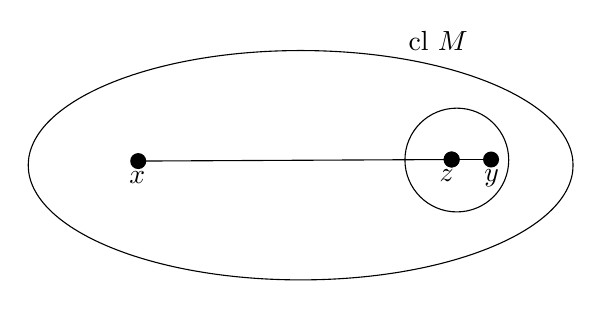
\begin{tikzpicture}[x=0.75pt,y=0.75pt,yscale=-1,xscale=1]
%uncomment if require: \path (0,300); %set diagram left start at 0, and has height of 300

%Straight Lines [id:da13368339552233044] 
\draw    (99.5,111) -- (250.5,110.25) ;
\draw [shift={(250.5,110.25)}, rotate = 359.72] [color={rgb, 255:red, 0; green, 0; blue, 0 }  ][fill={rgb, 255:red, 0; green, 0; blue, 0 }  ][line width=0.75]      (0, 0) circle [x radius= 3.35, y radius= 3.35]   ;
\draw [shift={(99.5,111)}, rotate = 359.72] [color={rgb, 255:red, 0; green, 0; blue, 0 }  ][fill={rgb, 255:red, 0; green, 0; blue, 0 }  ][line width=0.75]      (0, 0) circle [x radius= 3.35, y radius= 3.35]   ;
%Straight Lines [id:da21549014047251047] 
\draw    (250.5,110.25) -- (269.5,110.25) ;
\draw [shift={(269.5,110.25)}, rotate = 0] [color={rgb, 255:red, 0; green, 0; blue, 0 }  ][fill={rgb, 255:red, 0; green, 0; blue, 0 }  ][line width=0.75]      (0, 0) circle [x radius= 3.35, y radius= 3.35]   ;
\draw [shift={(250.5,110.25)}, rotate = 0] [color={rgb, 255:red, 0; green, 0; blue, 0 }  ][fill={rgb, 255:red, 0; green, 0; blue, 0 }  ][line width=0.75]      (0, 0) circle [x radius= 3.35, y radius= 3.35]   ;
%Shape: Ellipse [id:dp7644057548735066] 
\draw   (46.5,113) .. controls (46.5,82.49) and (105.26,57.75) .. (177.75,57.75) .. controls (250.24,57.75) and (309,82.49) .. (309,113) .. controls (309,143.51) and (250.24,168.25) .. (177.75,168.25) .. controls (105.26,168.25) and (46.5,143.51) .. (46.5,113) -- cycle ;
%Shape: Circle [id:dp7937136617849974] 
\draw   (228,110.5) .. controls (228,96.69) and (239.19,85.5) .. (253,85.5) .. controls (266.81,85.5) and (278,96.69) .. (278,110.5) .. controls (278,124.31) and (266.81,135.5) .. (253,135.5) .. controls (239.19,135.5) and (228,124.31) .. (228,110.5) -- cycle ;

% Text Node
\draw (94,114.73) node [anchor=north west][inner sep=0.75pt]    {$x$};
% Text Node
\draw (243.5,113.73) node [anchor=north west][inner sep=0.75pt]    {$z$};
% Text Node
\draw (265,113.73) node [anchor=north west][inner sep=0.75pt]    {$y$};
% Text Node
\draw (228.5,47) node [anchor=north west][inner sep=0.75pt]   [align=left] {cl $\displaystyle M$};


\end{tikzpicture}


\caption{Visualization of the proof}\label{fig:conx_proo}
\end{figure}

\end{proof}
\begin{proof}\color{ForestGreen} of \cref{cora:nnna}: 

``$\Rightarrow$'': obvious.

``$\Leftarrow$'': this is exactly the proof 2) above.

\end{proof}
\subsubsection{More Examples of Convex}
\begin{defa}{\bfs{Polyhedron}}
 See also  \cref{exm:polyh} for details
\end{defa}

\begin{exma}{\bfs{polytope: bounded polyhedron}}
A polytope can also be represented as (inner description) the convex hull of a finite nonempty set in $\mathbf{R}^{n}$, i.e., the set of the form
\begin{align*}
\operatorname{Conv}\left(\left\{u_{1}, \ldots, u_{N}\right\}\right)=\left\{\sum_{i=1}^{N} \lambda_{i} u_{i} \mid \lambda_{i} \geq 0, \sum_{i} \lambda_{i}=1\right\}
\end{align*}

\end{exma}
\begin{exma}{\bfs{simplex}}
 An important case of a polytope is a simplex, the convex hull of $n+1$ \tb{affinely independent} points $v_{1}, \ldots, v_{n+1}$ from $\mathbf{R}^{n}$ :
\begin{align*}
M=\operatorname{Conv}\left(\left\{v_{1}, \ldots, v_{n+1}\right\}\right)=\left\{\sum_{i=1}^{n+1} \lambda_{i} v_{i} \mid \lambda_{i} \geq 0, \sum_{i=1}^{n+1} \lambda_{i}=1\right\}
\end{align*}
the points $v_{1}, \ldots, v_{n+1}$ are called vertices of the simplex.
\end{exma}

\begin{exma}{\bfs{Euclidean balls and ellipsoids}}
(see \cref{exm:ball_ell} for another proof of convex and closed)

\tb{Euclidean balls:}
\begin{align*}
B\left(x_{c}, r\right)\coloneqq\left\{x \mid\left\|x-x_{c}\right\|_{2} \leq r\right\}=\left\{x \mid\left(x-x_{c}\right)^{\top}\left(x-x_{c}\right) \leq r^{2}\right\}
\end{align*}
where $r>0$, and $\|\cdot\|_{2}$ denotes the Euclidean norm
\begin{rema}{\bfs{equivalent form}}
\begin{align*}
B\left(x_{c}, r\right)=\left\{x_{c}+r u \mid\|u\|_{2} \leq 1\right\}
\end{align*}
\end{rema}
\tb{Ellipsoids:}
\begin{align*}
\mathcal{E}\coloneqq\left\{x \mid\left(x-x_{c}\right)^{\top} P^{-1}\left(x-x_{c}\right) \leq 1\right\}
\end{align*}
where $P=P^{\top} \succ 0$, i.e., $P$ is symmetric and positive definite. 
\begin{rema}{\bfs{equivalent form}}
\begin{align*}
\mathcal{E}=\left\{x_{c}+A u \mid\|u\|_{2} \leq 1\right\}
\end{align*}
where $A$ is square and nonsingular. In this representation we can assume without loss of generality that $A$ is symmetric and positive definite by taking $A=P^{1 / 2}$. When the matrix $A$ is symmetric positive semidefinite but singular, it is called a degenerate ellipsoid; its affine dimension is equal to the rank of $A$. Degenerate ellipsoids are also convex.
\end{rema}
\end{exma}
\begin{exma}{\bfs{Norm Cone}}
The norm cone associated with the any norm $\|\cdot\|$ is the set
\begin{align*}
C\coloneqq\{(x, t) \mid\|x\| \leq t\} \subseteq \mathbf{R}^{n+1}
\end{align*}
\end{exma}

\subsubsection{Generalized Inequalities}
\paragraph{Proper Cones and Generalized Inequalities}
\begin{defa}{\bfs{Proper Cone}}
 A convex cone $K \subseteq \mathbf{R}^{n}$ is called a proper cone if it satisfies the following:
\begin{itemize}
    \item $K$ is convex.
    \item $K$ is closed.
    \item $K$ is solid, which means it has nonempty interior.
    \item $K$ is pointed, which means that it contains no line (or equivalently, $x \in$ $K,-x \in K \Longrightarrow x=0)$
\end{itemize}
\end{defa}
\begin{defa}{\bfs{Generalized Inequality}}
 We associate with the proper cone $K$ the partial ordering on $\mathbf{R}^{n}$ defined by
\begin{align*}
x \preceq_{K} y \Longleftrightarrow y-x \in K
\end{align*}
We also write $x \succeq_{K} y$ for $y \preceq_{K} x$. Similarly, we define an associated strict partial ordering by
\begin{align*}
x \prec_{K} y \Longleftrightarrow y-x \in \operatorname{int} K
\end{align*}
and write $x \succ_{K} y$ for $y \prec_{K} x$.
\end{defa}
\tb{Properties of generalized inequalities:}

A generalized inequality $\preceq_{K}$ satisfies many properties, such as
\begin{itemize}
    \item $\preceq_{K}$ is preserved under addition: if $x \preceq_{K} y$ and $u \preceq_{K} v$, then $x+u \preceq_{K} y+v$.
    \item $\preceq_{K}$ is transitive: if $x \preceq_{K} y$ and $y \preceq_{K} z$ then $x \preceq_{K} z$.
    \item $\preceq_{K}$ is preserved under nonnegative scaling: if $x \preceq_{K} y$ and $\alpha \geq 0$ then $\alpha x \preceq_{K} \alpha y$
    \item $\preceq_{K}$ is reflexive: $x \preceq_{K} x$.
    \item $\preceq_{K}$ is antisymmetric: if $x \preceq_{K} y$ and $y \preceq_{K} x$, then $x=y$.
    \item $\preceq_{K}$ is preserved under limits: if $x_{i} \preceq_{K} y_{i}$ for $i=1,2, \ldots, x_{i} \rightarrow x$ and $y_{i} \rightarrow y$ as $i \rightarrow \infty$, then $x \preceq_{K} y$.
\end{itemize}

The corresponding strict generalized inequality $\prec_{K}$ satisfies, for example,
\begin{itemize}
    \item if $x \prec_{K} y$ then $x \preceq_{K} y$.
    \item if $x \prec_{K} y$ and $u \preceq_{K} v$ then $x+u \prec_{K} y+v$
    \item if $x \prec_{K} y$ and $\alpha>0$ then $\alpha x \prec_{K} \alpha y$.
    \item $x \nprec_{K} x$.
    \item if $x \prec_{K} y$, then for $u$ and $v$ small enough, $x+u \prec_{K} y+v$.
\end{itemize}
\paragraph{Minimum and Minimal Elements}
\begin{defa}{\bfs{Minimum}}
 We say that $x \in S$ is the \tb{minimum} element of $S$ (with respect to the generalized inequality $\preceq_{K}$ ) if for every $y \in S$ we have $x \preceq_{K} y$. We define the \tb{maximum} element of a set $S$, with respect to a generalized inequality, in a similar way. If a set has a minimum (maximum) element, then it is \tb{unique}.
\end{defa}
\begin{defa}{\bfs{Minimal}}
 We say that $x \in S$ is a \tb{minimal} element of $S$ (with respect to the generalized inequality $\preceq_{K}$ ) if $y \in S, y \preceq_{K} x$ only if $y=x$. We define \tb{maximal} element in a similar way. A set can have many different minimal (maximal) elements, so \tb{not unique.}
\end{defa}

\tb{\centerline{$x \in S$ is the minimum element of $S$ $\Longleftrightarrow$
$S \subseteq x+K$}}
Here $x+K$ denotes all the points that are comparable to $x$ and greater than or equal to $x$ (according to $\preceq_{K}$ ). 

\tb{\centerline{$x \in S$ is the minimal element of $S$ $\Longleftrightarrow$
$(x-K) \cap S=\{x\}$}}
Here $x-K$ denotes all the points that are comparable to $x$ and less than or equal to $x$ (according to $\preceq_{K}$ ); the only point in common with $S$ is $x$.

\subsection{The Separation Theorem}
In this section we answer the following question: assume we are given two convex sets $S$ and $T$ in $\mathbf{R}^n$, when can we separate them by a hyperplane.

\begin{defa}{\bfs{Hyperplane}}
 A hyperplane $M$ in $\mathbf{R}^{n}$ (an affine set of dimension $n-1$) is nothing but a level set of a nontrivial linear form:
\begin{align*}
\exists a \in \mathbf{R}^{n}, b \in \mathbf{R}, a \neq 0: \quad M=\left\{x \in \mathbf{R}^{n} \mid a^{\top} x=b\right\}
\end{align*}
\end{defa}
\begin{defa}{\bfs{Proper Separation}}
 We say that a hyperplane
\begin{align*}
M=\left\{x \in \mathbf{R}^{n} \mid a^{\top} x=b\right\} \quad[a \neq 0]
\end{align*}
properly separates (nonempty) convex sets $S$ and $T$, if
\begin{enumerate}[(i)]
    \item the sets belong to the opposite closed half-spaces into which $M$ splits $\mathbf{R}^{n}$
    \item  at least one of the sets is not contained in $M$ itself.
\end{enumerate}
We say that $S$ and $T$ can be \tb{properly separated}, if there exists a hyperplane which properly separates $S$ and $T$, i.e., if there exists $a \in \mathbf{R}^{n}$ such that
\begin{align*}
\sup _{x \in S} a^{\top} x \leq \inf _{y \in T} a^{\top} y \text{ ($\Leftrightarrow$ condition (i))}
\end{align*}
and
\begin{align*}
\inf _{x \in S} a^{\top} x<\sup _{y \in T} a^{\top} y \text{ ($\Leftrightarrow$ condition (ii))}
\end{align*}
\end{defa}
\begin{defa}{\bfs{Strong Separation}}
 We say that nonempty sets $S$ and $T$ in $\mathbf{R}^{n}$ can be strongly separated, if there exist two distinct parallel hyperplanes which separate $S$ and $T$, i.e., if there exists $a \in \mathbf{R}^{n}$ such that
\begin{align*}
\sup _{x \in S} a^{\top} x<\inf _{y \in T} a^{\top} y
\end{align*}
\end{defa} 
\begin{rema}
strong separation $\Rightarrow$ proper separation
\end{rema}
\begin{thma}{\bfs{Proper Separation Theorem}}\label{thm:sep_prop}
Two nonempty convex sets $S$ and $T$ in $\mathbf{R}^{n}$ can be properly separated if and only if their relative interiors do not intersect:
\begin{align*}
\text{\tb{convex sets $S$ and $T$ can be properly separated}} \Longleftrightarrow\operatorname{ri} S \cap \operatorname{ri} T=\emptyset
\end{align*}
\end{thma}
\begin{exma}{\bfs{separation of an affine and a convex set}}\label{exm:mnm}
   Suppose $C$ is convex and $D$ is affine, i.e., $D=\left\{F u+g \mid u \in \mathbf{R}^{m}\right\}$, where $F \in \mathbf{R}^{n \times m} .$ Suppose $C$ and $D$ are disjoint, so by the separating hyperplane theorem there are $a \neq 0$ and $\mu$ such that $a^{\top} x \leq \mu$ for all $x \in C$ and $a^{\top} x \geq \mu$ for all $x \in D$.
   
Now $a^{\top} x \geq \mu$ for all $x \in D$ means $a^{\top} F u \geq \mu-a^{\top} g$ for all $u \in \mathbf{R}^{m}$. But a linear function is bounded below on $\mathbf{R}^{m}$ only when it is zero, so we conclude $a^{\top} F=0$ (and hence, $\mu \leq a^{\top} g$).

Thus we conclude that $\exists a \neq 0$ such that $F^{\top} a=0$ and $a^{\top} x \leq \mu \leq a^{\top} g$ for all $x \in C$.
\end{exma}
\begin{exma}{\bfs{alternatives for strict linear inequalities}}\label{exm:mnm1}
 We derive the necessary conditions for solvability of a system of strict linear inequalities
\begin{align}
A x \prec b\label{eq:fdaffc}
\end{align}
These inequalities are infeasible if and only if the (convex) sets
\begin{align*}
C=\left\{b-A x \mid x \in \mathbf{R}^{n}\right\}, \quad D=\mathbf{R}_{++}^{m}=\left\{y \in \mathbf{R}^{m} \mid y \succ 0\right\}
\end{align*}
do not intersect. The set $D$ is open; $C$ is an affine set. Hence by the result above, $\exists \mu$, s.t. $A^{\top} \lambda=0$ and $\lambda^{\top} b \leq \mu .$ The second inequality means $\lambda^{\top} y \geq \mu$ for all $y \succ 0$. This implies $\mu \leq 0$ and $\lambda \succeq 0, \lambda \neq 0$. (This is because if $\lambda_i<0$, for large enough $y_i>0$, the inequality is wrong. If $\mu > 0$, for small enough $\alpha>0$, we have  $\lambda^{\top} \alpha y < \mu$.)

Putting it all together, we find: \cref{eq:fdaffc} is infeasible $\Longrightarrow$
\begin{align}
 \exists \lambda \text{ s.t. } \lambda \neq 0, \quad \lambda \succeq 0, \quad A^{\top} \lambda=0, \quad \lambda^{\top} b \leq 0\label{eq:nmvnm}
\end{align}
This is also a system of linear inequalities and linear equations in the variable $\lambda \in \mathbf{R}^{m}$. 
\end{exma}
\begin{rema}
Later in \cref{exm:fafdavcz}, we will show:

\centerline{\cref{eq:nmvnm}$\Longleftrightarrow$ ``\cref{eq:fdaffc} is infeasible''}
\end{rema}
\subsubsection{Necessity of Proper Separation Theorem: ``$\Rightarrow$''}
We first introduce a lemma about linear function and its maximum/minimum:
\begin{lema}\label{lem:lem_linear_min_cons}
``A linear function $f(x)=a^{\top} x$ can attain its maximum/minimum over a convex set $M$ at a point $\bar{x} \in \operatorname{ri} M$'' $\Longleftrightarrow$ ``the function is \tb{constant} on $M$''
\end{lema}
\begin{rema}
This lemma for the maximum will be generalized to constant of convex function in \cref{thm:max_convf}
\end{rema}
\begin{figure}[H]
\centering
\tikzset{every picture/.style={line width=0.75pt}} %set default line width to 0.75pt        

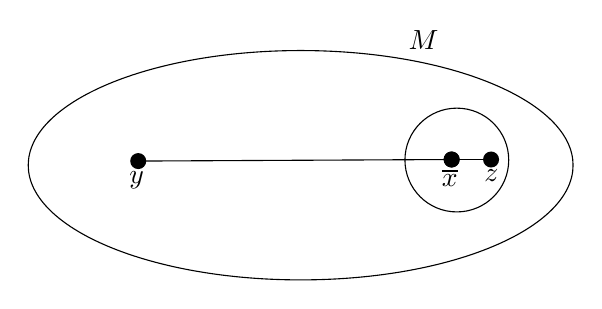
\begin{tikzpicture}[x=0.75pt,y=0.75pt,yscale=-1,xscale=1]
%uncomment if require: \path (0,300); %set diagram left start at 0, and has height of 300

%Straight Lines [id:da13368339552233044] 
\draw    (99.5,111) -- (250.5,110.25) ;
\draw [shift={(250.5,110.25)}, rotate = 359.72] [color={rgb, 255:red, 0; green, 0; blue, 0 }  ][fill={rgb, 255:red, 0; green, 0; blue, 0 }  ][line width=0.75]      (0, 0) circle [x radius= 3.35, y radius= 3.35]   ;
\draw [shift={(99.5,111)}, rotate = 359.72] [color={rgb, 255:red, 0; green, 0; blue, 0 }  ][fill={rgb, 255:red, 0; green, 0; blue, 0 }  ][line width=0.75]      (0, 0) circle [x radius= 3.35, y radius= 3.35]   ;
%Straight Lines [id:da21549014047251047] 
\draw    (250.5,110.25) -- (269.5,110.25) ;
\draw [shift={(269.5,110.25)}, rotate = 0] [color={rgb, 255:red, 0; green, 0; blue, 0 }  ][fill={rgb, 255:red, 0; green, 0; blue, 0 }  ][line width=0.75]      (0, 0) circle [x radius= 3.35, y radius= 3.35]   ;
\draw [shift={(250.5,110.25)}, rotate = 0] [color={rgb, 255:red, 0; green, 0; blue, 0 }  ][fill={rgb, 255:red, 0; green, 0; blue, 0 }  ][line width=0.75]      (0, 0) circle [x radius= 3.35, y radius= 3.35]   ;
%Shape: Ellipse [id:dp7644057548735066] 
\draw   (46.5,113) .. controls (46.5,82.49) and (105.26,57.75) .. (177.75,57.75) .. controls (250.24,57.75) and (309,82.49) .. (309,113) .. controls (309,143.51) and (250.24,168.25) .. (177.75,168.25) .. controls (105.26,168.25) and (46.5,143.51) .. (46.5,113) -- cycle ;
%Shape: Circle [id:dp7937136617849974] 
\draw   (228,110.5) .. controls (228,96.69) and (239.19,85.5) .. (253,85.5) .. controls (266.81,85.5) and (278,96.69) .. (278,110.5) .. controls (278,124.31) and (266.81,135.5) .. (253,135.5) .. controls (239.19,135.5) and (228,124.31) .. (228,110.5) -- cycle ;

% Text Node
\draw (94,114.73) node [anchor=north west][inner sep=0.75pt]    {$y$};
% Text Node
\draw (244.5,113.73) node [anchor=north west][inner sep=0.75pt]    {$\overline{x}$};
% Text Node
\draw (265,113.73) node [anchor=north west][inner sep=0.75pt]    {$z$};
% Text Node
\draw (228.5,47) node [anchor=north west][inner sep=0.75pt]   [align=left] {$\displaystyle M$};


\end{tikzpicture}

\caption{Visualization of the proof}\label{fig:conx_proo1}
\end{figure}

\begin{proof}\color{ForestGreen}
"$\Leftarrow$" part is evident. To prove the "$\Rightarrow$" part, let $\bar{x} \in$ ri $M$ be, say, a minimizer of $f$ over $M$, we need to prove that $f(\bar{x})=f(y), \forall y\in M$ and $y\ne x$. 

Since $\bar{x} \in \ri M$, the segment $[y, \bar{x}]$, which is contained in $M$, can be extended a little bit through the point $\bar{x}$, not leaving $M$ (since $\bar{x} \in$ ri $M)$, so that there exists $z \in M$ such that $\bar{x} \in(y, z)$, i.e., $\bar{x}=(1-\lambda) y+\lambda z$ with certain $\lambda \in(0,1) .$ Since $f$ is linear, we have
\begin{align}
f(\bar{x})=(1-\lambda) f(y)+\lambda f(z).\label{eq:tydi}
\end{align}
Since $f(\bar{x}) \leq \min \{f(y), f(z)\}$ and $0<\lambda<1$, the about equality can be satisfied only when $f(\bar{x})=f(y)=f(z)$. If $\bar{x}$ is a maximizer, the proof is similar.

\end{proof}

Assume that the sets can be properly separated with one $a$:
\begin{align}
\sup _{x \in S} a^{\top} x \leq \inf _{y \in T} a^{\top} y ; \quad \inf _{x \in S} a^{\top} x<\sup _{y \in T} a^{\top} y\label{eq:bmnv}
\end{align}
Assume there exists a point $\bar{x} \in(\operatorname{ri} S \cap \operatorname{ri} T)$,  then from the first inequality in \cref{eq:bmnv} it is clear that $\bar{x}$ maximizes the linear function $f(x)=a^{\top} x$ on $S$ and at the same time, it minimizes this form on $T$. According to \cref{lem:lem_linear_min_cons}, the second inequality cannot be correct in \cref{eq:bmnv}.

We therefore have ``$\Rightarrow$'' in \cref{thm:sep_prop}.

\subsubsection{Sufficiency of Proper Separation Theorem: ``$\Leftarrow$''}
\paragraph{Separate Closed Convex Set and Point Outside:}
\begin{lema}{\bfs{strong separation of closed convex set and point outside}}\label{lem:sep_con_pointnotin}
Let $M$ be a nonempty and \tb{closed convex} set in $\mathbf{R}^{n}$, and let $x$ be $a$ point outside $M(x \notin M) .$ Consider the optimization program
\begin{align}
\min \{||x-y||_2 \mid y \in M\}\label{eq:opt_mina}
\end{align}
The program is solvable and has a unique solution $y^{*}$, and the linear form $a^{\top} h, a=x-y^{*}$ \tb{strongly separates} $x$ and $M:$
\begin{align*}
\sup _{y \in M} a^{\top} y=a^{\top} y^{*}=a^{\top} x-|a|^{2}< a^{\top}x 
\end{align*}
The point $y^{*}$ is called \tb{projection} of $x$ on $M .$ 
\end{lema}
\begin{figure}[H]
\centering
\tikzset{every picture/.style={line width=0.75pt}} %set default line width to 0.75pt        

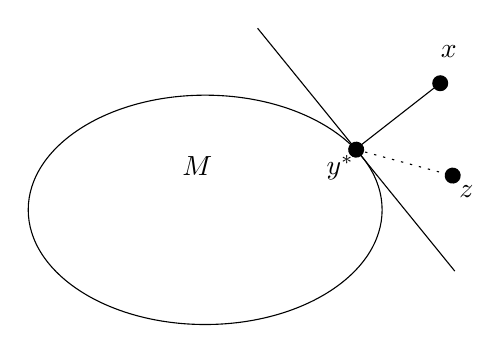
\begin{tikzpicture}[x=0.75pt,y=0.75pt,yscale=-1,xscale=1]
%uncomment if require: \path (0,300); %set diagram left start at 0, and has height of 300

%Shape: Ellipse [id:dp7644057548735066] 
\draw   (45.5,114) .. controls (45.5,83.49) and (83.67,58.75) .. (130.75,58.75) .. controls (177.83,58.75) and (216,83.49) .. (216,114) .. controls (216,144.51) and (177.83,169.25) .. (130.75,169.25) .. controls (83.67,169.25) and (45.5,144.51) .. (45.5,114) -- cycle ;
%Straight Lines [id:da32241885713234253] 
\draw    (156,26.5) -- (251,143.5) ;
\draw [shift={(203.5,85)}, rotate = 50.92] [color={rgb, 255:red, 0; green, 0; blue, 0 }  ][fill={rgb, 255:red, 0; green, 0; blue, 0 }  ][line width=0.75]      (0, 0) circle [x radius= 3.35, y radius= 3.35]   ;
%Straight Lines [id:da9297235482273263] 
\draw    (244,53) ;
\draw [shift={(244,53)}, rotate = 0] [color={rgb, 255:red, 0; green, 0; blue, 0 }  ][fill={rgb, 255:red, 0; green, 0; blue, 0 }  ][line width=0.75]      (0, 0) circle [x radius= 3.35, y radius= 3.35]   ;
%Straight Lines [id:da6355849350039298] 
\draw    (203,85) -- (244,53) ;
%Straight Lines [id:da37403627562052844] 
\draw  [dash pattern={on 0.84pt off 2.51pt}]  (203.5,85) -- (250,97.5) ;
\draw [shift={(250,97.5)}, rotate = 15.05] [color={rgb, 255:red, 0; green, 0; blue, 0 }  ][fill={rgb, 255:red, 0; green, 0; blue, 0 }  ][line width=0.75]      (0, 0) circle [x radius= 3.35, y radius= 3.35]   ;

% Text Node
\draw (243,33.73) node [anchor=north west][inner sep=0.75pt]    {$x$};
% Text Node
\draw (118.5,87) node [anchor=north west][inner sep=0.75pt]   [align=left] {$\displaystyle M$};
% Text Node
\draw (188,86.73) node [anchor=north west][inner sep=0.75pt]    {$y^{*}$};
% Text Node
\draw (252,100.9) node [anchor=north west][inner sep=0.75pt]    {$z$};


\end{tikzpicture}

\caption{Visualization of the proof}\label{fig:conx_proo2}
\end{figure}
\begin{proof}\color{ForestGreen}
Sketch: We know \cref{eq:opt_mina} is bounded below with infimum $m>0$ ($>0$ if from outside closed set). Denote $f(y)\coloneqq ||x-y||_2$. Set $N\coloneqq\{y\mid f(y)\le 2m\}$ is closed and bounded as therefore compact. $M\cap N$ is therefore compact. We can achieve the infimum $m$ with $y=y^*$. 

Uniqueness is from the strong convexity of norm function: if $f(y')=f(y^*)$, we have a point $y''$ in seg $[y',y^*]$ and  $f(y'')<f(y')$. 

We next prove $\sup _{y \in M} a^{\top} y=a^{\top} y^{*}$: if not true, we have a $z\in M$ s.t. $a^{\top} y^{*}<a^{\top} z$, i.e. $a^{\top} (y^{*}-z)<0$, however this geometrically means $\exists y'\in \text{segment }(y^*,z)$ s.t. $f(y')<f(y^*)$.
\end{proof}

Let us consider an example of application of the above proposition:
\begin{cora}\bfs{support function and convex set}\label{cora:sfcs}
Let $M$ be a convex set. Consider a function
\begin{align}
\psi_{M}(x)=\sup \left\{y^{\top} x \mid y \in M\right\}\label{eq:supp_def}
\end{align}
Function $\psi_{M}(x)$ is called the \tb{support function} of the set $M$.
Now, let $M_{1}$ and $M_{2}$ be two closed convex sets.
\begin{enumerate}
    \item If for any $x \in \dom \psi_{M_{2}}$ we have $\psi_{M_{1}}(x) \leq \psi_{M_{2}}(x)$ then $M_{1} \subset M_{2}$.
    \item If $\dom \psi_{M_{1}}=\dom \psi_{M_{2}}$ and for any $x \in \dom \psi_{M_{1}}$ we have $\psi_{M_{1}}(x)=\psi_{M_{2}}(x) .$ Then $M_{1} \equiv M_{2}$.
\end{enumerate}
\end{cora} 
\begin{rema}
The support function will be used in \cref{sec:sub_cal}.
\end{rema}
\begin{proof}\color{ForestGreen}
For 1), assume, on the contrary, that there is $x_{0} \in M_{1}$ and $x_{0} \notin M_{2} .$ From \cref{lem:sep_con_pointnotin}, we know there is $a \neq 0$ such that $a^{\top} x_{0}>a^{\top} x$ for any $x \in M_{2} .$ Hence, $a \in \dom \psi_{M_{2}}$ because $sup_x a^\top x $is bounded, and $\psi_{M_{1}}(a)>\psi_{M_{2}}(a)$, which is a contradiction. 2) is a direct conclusion from 1).
\end{proof}
\begin{rema}
Supporting function $\psi_{M}(x)$ for any $M$ (not necessarily convex) is positively homogenous of degree 1 :
\begin{align*}
\psi_{M}(t x)=t \psi_{M}(x), \quad x \in \dom \psi_{M}, \quad t \geq 0
\end{align*}
and if the set $M$ is bounded then $\dom \psi_{M}=\mathbf{R}^{n}$
\end{rema}
\paragraph{Separate Convex Set and Non-Interior Point}
Now we consider a point outside the relative interior of a convex (\tb{not necessarily closed}) set. In general, we do not have strong separation, but still have the proper separation.
\begin{lema}{\bfs{Separation of a point and a set}}\label{lem:sep_con_point_p}
Let $M$ be a convex set in $\mathbf{R}^{n}$, and let $x \notin \ri M$. Then $x$ and $M$ can be properly separated.
\end{lema}
\begin{proof}\color{ForestGreen}
$\cl M$ is a closed convex set with the same relative interior as that of $M$, and  $x \notin \ri \cl M$.
 
If $x \notin \cl M$, then $x$ and $\cl M$ (and also $x$ and $M \subset \cl M)$ can be strongly  separated by \cref{lem:sep_con_pointnotin}. 

If $x$ is a point of relative boundary of $\cl M: x \in \partial_{\mathrm{ri}} \cl M \equiv \cl M \backslash \ri \cl M$. Without loss of generality we may assume that $x=0$ (simply by translation). Let $L$ be the linear span of $M$. Similar to the proof in \cref{thm:cox_cl_ri}, we may restrict our attention to the subspace $L$. 

Since $x=0$ is not in the relative interior of $\cl M$, there is a sequence of points $x_{i}\in L$ not belonging to $\cl M$ and converging to $0$ and each $x_{i}$ can be strongly separated from $\cl M$: there exists a linear form $a_{i}^{\top} x$ with the property
\begin{align*}
a_{i}^{\top} x_{i}<\inf _{y \in \cl M} a_{i}^{\top} y
\end{align*}
By normalization, we can assume that all $a_i$ belong to the unit ball. i.e., to a compact set. By resorting to a subsequence, we may assume that $a_{i}$ themselves converge to certain vector $a \in L$. This vector is unit, since all $a_{i}$ 's are unit. Now, we have for every fixed $y \in \cl M:$
\begin{align*}
a_{i}^{\top} x_{i}<a_{i}^{\top} y
\end{align*}
As $i \rightarrow \infty$, we have $a_{i} \rightarrow a, x_{i} \rightarrow x=0$, and passing to limit in our inequality, we get
\begin{align*}
a^{\top} x=0 \leq a^{\top} y, \quad \forall y \in \cl M
\end{align*}
Thus, we have established the main part of the required statement: the linear form $f(u)=$ $a^{\top} u$ separates $\{0\}$ and $\cl M$ (and thus $\{0\}$ and $\left.M \subset \cl M\right) .$ It remains to verify that this separation is proper, which in our case simply means that $M$ is not contained in the hyperplane $\left\{u \mid a^{\top} u=0\right\} .$ But this is evident since $a\in L =\Aff (M)$.
\end{proof}
\paragraph{The General Case}
Given two nonempty convex sets $S$ and $T$ with the non-intersecting relative interiors, and we should prove that the sets can be properly separated. 

Let $S^{\prime}=\operatorname{ri} S, T^{\prime}=\operatorname{ri} T ;$ these are two nonempty convex sets and they do not intersect. Let $M=T^{\prime}-S^{\prime}=\left\{z=x-y \mid x \in T^{\prime}, y \in S^{\prime}\right\}$ which is a nonempty convex (as a sum of two nonempty convex sets) set which does not contain $0$. By \cref{lem:sep_con_point_p}, $\{0\}$ and $M$ can be properly separated: there exists $a$ such that
\begin{align*}
0=a^{\top} 0 \leq \inf _{z \in M} a^{\top} z \equiv \inf _{y \in T^{\prime}, x \in S^{\prime}} a^{\top}(y-x)=\left[\inf _{y \in T^{\prime}} a^{\top} y\right]-\left[\sup _{x \in S^{\prime}} a^{\top} x\right]
\end{align*}
and
\begin{align*}
0<\sup _{z \in M} a^{\top} z \equiv \sup _{y \in T^{\prime}, x \in S^{\prime}} a^{\top}(y-x)=\left[\sup _{y \in T^{\prime}} a^{\top} y\right]-\left[\inf _{x \in S^{\prime}} a^{\top} x\right]
\end{align*}
From \cref{thm:cox_cl_ri}, we have
\begin{align*}
\sup _{x \in S} a^{\top} x \leq \inf _{y \in T} a^{\top} y, \inf _{x \in S} a^{\top} x<\sup _{y \in T} a^{\top} y
\end{align*}
which means proper separation of $S$ and $T$.
\subsubsection{Strong Separation}
There is also a simple \tb{necessary and sufficient} condition for two sets to be \tb{strongly separated}:
\begin{lema}
Two nonempty convex sets $S$ and $T$ in $\mathbf{R}^{n}$ can be strongly separated if and only if:
\begin{align*}
\rho(S, T)=\inf _{x \in S, y \in T}|x-y|>0
\end{align*}
One special case is one of the sets is compact, the other one is closed and the sets do not intersect.
\end{lema} 
\begin{proof}\color{ForestGreen}
''$\Leftarrow$'': if $S$ and $T$ can be strongly separated, i.e., for certain $a$ one has
\begin{align*}
\alpha \equiv \sup _{x \in S} a^{\top} x<\beta \equiv \inf _{y \in T} a^{\top} y
\end{align*}
then from Cauchy's inequality for every pair $(x, y)$ with $x \in S$ and $y \in T$ one has
\begin{align*}
|x-y| \geq \frac{\beta-\alpha}{|a|}
\end{align*}

''$\Rightarrow$'':  consider the set $\Delta=S-T$. This is a convex set which clearly does not contain vectors of the length less than $\rho(S, T)>0$; consequently, it does not intersect the ball $B$ of a radius $r<\rho(S, T)$ centered at the origin. Consequently, by the Separation Theorem, $\Delta$ can be properly separated from $B:$ there exists $a$ such that
\begin{align*}
\inf _{z \in B} a^{\top} z \geq \sup _{x \in S, y \in T} a^{\top}(x-y), \qquad \sup _{z \in B} a^{\top} z>\inf _{x \in S, y \in T} a^{\top}(x-y)
\end{align*}
From the second of these inequalities it follows that $a \neq 0$. Therefore $\inf _{z \in B} a^{\top} z<0$, so that the first inequality in  means that $a$ strongly separates $S$ and $T$.
\end{proof}

\subsubsection{Outer Description of Closed Convex Set: supporting planes}\label{sec:out_conx}
We can now prove the "outer" characterization of a closed convex set announced in the beginning of this section:

\begin{thma}{\bfs{outer description of closed convex set}}
Any closed convex set $M$ in $\mathbf{R}^{n}$ is the solution set of an (infinite) system of nonstrict linear inequalities.

Geometrically: every closed convex set $M \subset \mathbf{R}^{n}$ which differs from the entire $\mathbf{R}^{n}$ is the intersection of all closed half-spaces which contain $M$.
\end{thma}
\begin{rema}
If $M$ is convex but not necessarily closed, intersection of all closed half-spaces which contain $M$ is $\cl M$. 
\end{rema}
\begin{proof}\color{ForestGreen}
If $M$ is empty, there is nothing to prove: an empty set is the intersection of two properly chosen closed half-spaces. If $M$ is the entire space, there also is nothing to prove: this is the solution set to the empty system of linear inequalities. Now assume that $M$ is convex, closed, nonempty and differs from the entire space. Let $x \notin M ;$ then $x$ is at the positive distance from $M$ since $M$ is closed and therefore there exists a hyperplane strongly separating $x$ and $M$:
\begin{align*}
\forall x \notin M \exists a_{x}: a_{x}^{\top} x>\alpha_{x} \equiv \sup _{y \in M} a_{x}^{\top} y
\end{align*}
For every $x \notin M$ the closed half-space $H_{x}=\left\{y \mid a_{x}^{\top} y \leq \alpha_{x}\right\}$ clearly contains $M$ and does not contain $x$; consequently,
\begin{align*}
M=\cap_{x \notin M} H_{x}
\end{align*}
\end{proof}

Among the closed half-spaces which contain a closed convex and proper (i.e., nonempty and differing from the entire space) set $M$ the most interesting are the "extreme" ones those with the boundary hyperplane touching $M$. The notion makes sense for an arbitrary (not necessary closed) convex set, but we will use it for closed sets only.

\begin{defa}{\bfs{Supporting Plane}}\label{def:supp_p}
  Let $M$ be a convex closed set in $\mathbf{R}^{n}$, and let $x\in \partial_{\mathrm{ri}} M$. A hyperplane
\begin{align*}
\Pi=\left\{y \mid a^{\top} y=a^{\top} x\right\} \quad[a \neq 0]
\end{align*}
is called \tb{supporting} to $M$ at $x$, if it properly separates $M$ and $\{x\}$, i.e., if
\begin{align*}
a^{\top} x \geq \sup _{y \in M} a^{\top} y\quad \text{and} \quad a^{\top} x>\inf _{y \in M} a^{\top} y
\end{align*}
\end{defa}
\begin{rema}{\bfs{equivalent definition}}
Note that since $x$ is a point from the relative boundary of $M$ and therefore belongs to $\cl M=M$, the first inequality is in fact is equality. Thus, an equivalent definition of a supporting plane is as follows:

Let $M$ be a closed convex set and $x\in \partial_{\mathrm{ri}} M$. The hyperplane $\left\{y \mid a^{\top} y=a^{\top} x\right\}$ is called supporting to $M$ at $x$, if the linear form $a(y)=a^{\top} y$:
\begin{enumerate}[i).]
    \item \tb{attain the maximum} on $M$ at the point $x$ 
    \item \tb{nonconstant} on $M$
\end{enumerate}
\end{rema}

The most important property of a supporting plane is its existence:
\begin{lema}{\bfs{existence of supporting hyperplane}}\label{lem:exis_supp_p}
 Let $M$ be a convex closed set in $\mathbf{R}^{n}$ and  $x\in \partial_{\mathrm{ri}} M$. Then
 \begin{enumerate}
     \item There exists at least one hyperplane which is supporting to $M$ at $x$;
     \item  If $\Pi$ is supporting to $M$ at $x$, then the intersection $M \cap \Pi$ is of affine dimension less than  the affine dimension of $M$.
 \end{enumerate}
\end{lema}
\begin{proof}\color{ForestGreen}
1). is easy from Proper Separation Theorem \cref{thm:sep_prop}.

To prove 2)., note that if $\Pi=\left\{y \mid a^{\top} y=a^{\top} x\right\}$ is supporting to $M$ at $x \in \partial_{\mathrm{ri}} M$, then the set $M^{\prime}=M \cap \Pi$ is nonempty (it contains $x$ ) convex set, and the linear form $a^{\top} y$ is constant on $M^{\prime}$ and therefore (why?) on the affine hull $M^{\prime}$. At the same time, the form is nonconstant on $M$ by definition of a supporting plane. Thus, Aff $\left(M^{\prime}\right)$ is a proper (less than the entire Aff $(M))$ subset of Aff $(M)$), and therefore the affine dimension of $M^{\prime}$ is less than the affine dimension of $M$\footnote{we used the following fact: if $P \subset M$ are two affine sets, then the affine dimension of $P$ is $\leq$ the one of $M$, with $\leq$ being $=$ if and only if $P=M$.}.
\end{proof} 


\subsection{Minimal Representation of Convex Sets: extreme points}
Extreme point of a convex set $M$ is a point in $M$ which cannot be obtained as a convex combination of other points of the set and set of all extreme points is the smallest set of points for which $M$ is the convex hull.
\begin{defa}{\bfs{Extreme Points}}
  Let $M$ be a nonempty convex set in $\mathbf{R}^{n}$. A point $x \in M$ is called an \tb{extreme point} of $M$, if there is no nontrivial (of positive length) segment $[u, v] \in M$ for which $x$ is an interior point, i.e., if we have
\begin{align*}
``x=\lambda u+(1-\lambda) v  \lambda \in(0,1), u,v\in M"\Rightarrow  ``u=v=x"
\end{align*}
\end{defa}

An equivalent statement of an extreme point is as follows:
\begin{lema}{\bfs{Equivalence}}
 A point $x$ in a convex set $M$ is extreme if and only if the set $M \backslash\{x\}$ is convex.
\end{lema}
\begin{proof}\color{ForestGreen}
easy
\end{proof}
We start with 2 lemmas:
\begin{lema}\label{lem:allline}
 Let $M$ be a closed convex set in $\mathbf{R}^{n} .$ Assume that for some $\bar{x} \in M$ and $h \in \mathbf{R}^{n} M$ contains the ray
\begin{align*}
\{\bar{x}+t h \mid t \geq 0\}
\end{align*}
starting at $\bar{x}$ with the direction $h$. Then $M$ contains also all parallel rays starting at the points of $M:$
\begin{align*}
\forall x \in M:\{x+t h \mid t \geq 0\} \subset M
\end{align*}
In particular, if $M$ contains certain line, then it contains also all parallel lines passing through the points of $M$.

\end{lema} 
\begin{defa}{\bfs{Recessive Direction}}\label{def:recessive_dir}
  For a convex set $M$, the directions $h$ such that $x+t h \in M$ for some (and thus for all) $x \in M$ and all $t \geq 0$ are called \tb{recessive} for $M$. Later in \cref{sec:conx_f}, we need this concept.
\end{defa}

\begin{proof}\color{ForestGreen}
If $x \in M$ and $\bar{x}+t h \in M$ for all $t \geq 0$ then, due to convexity, for any fixed $\tau \geq 0$ we have
\begin{align*}
\epsilon\left(\bar{x}+\frac{\tau}{\epsilon} h\right)+(1-\epsilon) x \in M
\end{align*}
for all $\epsilon \in(0,1)$. As $\epsilon \rightarrow+0$, the left hand side tends to $x+\tau h$, and since $M$ is closed, $x+\tau h \in M$ for every $\tau \geq 0$
\end{proof}
\begin{lema}\label{lem:ex_p}
  Let $M$ be a \tb{closed} convex set, $\bar{x}\in \partial_{\mathrm{ri}} M$ and $\Pi$ be a hyperplane supporting to $M$ at $\bar{x}$. Then all extreme points of the nonempty closed convex set $\Pi \cap M$ are extreme points of $M$.
\end{lema}
\begin{proof}\color{ForestGreen}
The set $\Pi \cap M$ is closed, convex and nonempty (contains $\bar{x}$). Let $a$ be the linear form associated with $\Pi$ :
\begin{align*}
\Pi=\left\{y \mid a^{\top} y=a^{\top} \bar{x}\right\}
\end{align*}
so that
\begin{align*}
\inf _{x \in M} a^{\top} x<\sup _{x \in M} a^{\top} x=a^{\top} \bar{x}
\end{align*}
from \cref{def:supp_p}. Assume that $y$ is an extreme point of $\Pi \cap M ;$ what we should do is to prove that
\begin{align*}
y=\lambda u+(1-\lambda) v
\end{align*}
for some $u, v \in M$ and $\lambda \in(0,1)$ is possible only if $y=u=v .$ To this end it suffices to prove $u, v \in \Pi \cap M$ (or, which is the same, to prove that $u, v \in \Pi$, since the points are known to belong to $M$ ). 
Note that since $y \in \Pi$ we have
\begin{align*}
a^{\top} y=a^{\top} \bar{x} \geq \max \left\{a^{\top} u, a^{\top} v\right\}
\end{align*}
On the other hand,
\begin{align*}
a^{\top} y=\lambda a^{\top} u+(1-\lambda) a^{\top} v
\end{align*}
combining these observations and taking into account that $\lambda \in(0,1)$, we conclude that
\begin{align*}
a^{\top} y=a^{\top} u=a^{\top} v
\end{align*}
But these equalities imply that $u, v \in \Pi$.
\end{proof}

\begin{thma}\label{thm:kthma}
Let $M$ be a \tb{closed} and nonempty convex set in $\mathbf{R}^{n} .$ Then
\begin{enumerate}[i).]
    \item The set $\operatorname{Ext}(M)$ of extreme points of $M$ is nonempty $\Longleftrightarrow$ $M$ does not contain lines;
    \item (KreinMilman Theorem) If $M$ is \tb{bounded}, then $M$ is the convex hull of its extreme points:
\begin{align*}
M=\operatorname{Conv}(\operatorname{Ext}(M))
\end{align*}
so that every point of $M$ is a convex combination of the points of $\operatorname{Ext}(M)$.
\end{enumerate}
\end{thma} 
\begin{proof}\color{ForestGreen}
Proof of i).

"$\Rightarrow$": If $M$ contains a line, then, by \cref{lem:allline}, there is a line in $M$ passing through any given point of $M$, so that no point can be extreme.

"$\Leftarrow$": We use \tb{induction on the dimension} of the convex set $M$.
There is nothing to do if the dimension of $M$ is zero, i.e., if $M$ is a point. Now assume that we already have proved the nonemptiness of $\operatorname{Ext}(T)$ for all nonempty closed and not containing lines convex sets $T$ of certain dimension $k$, and let us prove that the same statement is valid for the sets of dimension $k+1$. Let $M$ be a closed convex nonempty and not containing lines set of dimension $k+1$. Since the dimension of $M$ is positive $(k+1)$, $\rb M$ is not empty. Since $M$ does not contain lines and is of positive dimension, it differs from entire Aff $(M)$ and therefore it possesses a relative boundary point $\bar{x}$. Indeed, there exists $z \in \operatorname{Aff}(M) \backslash M$, so that the points
\begin{align*}
x_{\lambda}=x+\lambda(z-x),
\end{align*}
where $x$ is an arbitrary fixed point of $M$, do not belong to $M$ for some $\lambda \geq 1$, while $x_{0}=x$ belongs to $M$. The set of those $\lambda \geq 0$ for which $x_{\lambda} \in M$ is therefore nonempty and bounded from above; this set clearly is \tb{closed} (since $M$ is closed). Thus, there exists the largest $\lambda=\lambda^{*}$ for which $x_{\lambda} \in M$. 

We claim that $x_{\lambda^{*}}\in \rb M .$ Indeed, by construction this is a point from $M$. If $x\in \ri M$, all the points $x_{\lambda}$ with close to $\lambda^{*}$ and greater than $\lambda^{*}$ values of $\lambda$ would also belong to $M$, which contradicts the origin of $\lambda^{*}$.

According to \cref{lem:exis_supp_p} 1), there exists hyperplane $\Pi=\left\{x \mid a^{\top} x=a^{\top} \bar{x}\right\}$ which supports $M$ at $\bar{x}$ :
\begin{align*}
\inf _{x \in M} a^{\top} x<\max _{x \in M} a^{\top} x=a^{\top} \bar{x}
\end{align*}
By \cref{lem:exis_supp_p} 2)., the set $T=\Pi \cap M$ (which is closed, convex and nonempty) is of affine dimension less than that of $M$,  which clearly does not contain lines (since even the larger set $M$ does not contain lines). By Inductive Hypothesis, $T$ possesses extreme points, and by \cref{lem:ex_p} all these points are extreme also for $M$ The inductive step is complete, and (i) is proved.

Proof of ii).

What is immediately seen is that the right hand side set is contained in the left hand side one. Thus, all we need is to prove that any $x \in M$ is a convex combination of points from $\operatorname{Ext}(M)$. Here we again use \tb{induction on the dimension} of $M$. The case of $0$-dimensional set $M$ (i.e., a point) is trivial. Assume that the statement in question is valid for all $k$ dimensional convex closed and bounded sets, and let $M$ be a convex closed and bounded set of dimension $k+1$.

Let $x \in M$. To represent $x$ as a convex combination of points from $\operatorname{Ext}(M)$, let us pass through $x$ an arbitrary line $l=\{x+\lambda h \mid \lambda \in \mathbf{R}\}(h \neq 0)$ in the $\Aff (M)$. Moving along this line from $x$ in each of the two possible directions, we eventually leave $M$ (since $M$ is bounded); as it was explained in the proof of (i), it means that there exist nonnegative $\lambda_{+}$and $\lambda_{-}$such that the points
\begin{align*}
\bar{x}_{\pm}=x+\lambda_{\pm} h
\end{align*}
both belong to the boundary of $M$. Let us verify that $\bar{x}_{\pm}$are convex combinations of the extreme points of $M$ (this will then complete the proof). Indeed, $M$ admits supporting at $\bar{x}_{+}$hyperplane $\Pi ;$ and the set $\Pi \cap M$ (which clearly is convex, closed and bounded) is of less dimension than that one of $M$; by the inductive hypothesis, the point $\bar{x}_{+}$of this set is a convex combination of extreme points of the set, and by \cref{lem:ex_p} all these extreme points are extreme points of $M$ as well. Thus, $\bar{x}_{+}$is a convex combination of extreme points of $M$. Similar reasoning is valid for $\bar{x}_{-}$.
\end{proof}


\subsubsection{Application: extreme points of a polyhedral set}
Consider a polyhedral set
\begin{align*}
K=\left\{x \in \mathbf{R}^{n} \mid A x \leq b\right\}
\end{align*}
$A$ being a $m \times n$ matrix and $b$ being a vector from $\mathbf{R}^{m}$. What are the extreme points of $K ?$ The answer is given by the following
\begin{thma}{\bfs{extreme points of polyhedral set]}}
Let $x \in K$. The vector $x$ is an extreme point of $K$ $\Longleftrightarrow$ some $n$ \tb{linearly independent} (i.e., with linearly independent vectors of coefficients) inequalities of the system $A x \leq b$ are equalities at $x$.
\end{thma}
\begin{proof}\color{ForestGreen}
Let $a_{i}, i=1, \ldots, m$, be the the rows of $A$.

"$\Rightarrow$" part: let $x$ be an extreme point of $K$, and let $I$ be the set of those indices $i$ for which $a_{i}^{\top} x=b_{i}$; we should prove that the set $F$ of vectors $\left\{a_{i} \mid i \in I\right\}$ contains $n$ linearly independent vectors, or, which is the same, that linear span of $F$ is $\mathbf{R}^{n}$. Assume that it is not the case; then the orthogonal complement to $F$ contains a nonzero vector $h$. Consider the segment $\Delta_{\epsilon}=[x-\epsilon h, x+\epsilon h], \epsilon>0$ being the parameter of our construction. Since $h$ is orthogonal to the "active" vectors $a_{i}$, $i \in I$, all points $y$ of this segment satisfy the relations $a_{i}^{\top} y=a_{i}^{\top} x=b_{i}$. Now, if $i$ is a "nonactive" index with $a_{i}^{\top} x<b_{i}$, then $a_{i}^{\top} y \leq b_{i}$ for all $y \in \Delta_{\epsilon}$ provided that $\epsilon$ is small enough. Since there are finitely many nonactive indices, we can choose $\epsilon>0$ in such a way that all $y \in \Delta_{\epsilon}$ will satisfy all "nonactive" inequalities $a_{i}^{\top} x \leq b_{i}, i \notin I$. Since $y \in \Delta_{\epsilon}$ satisfies, as we have seen, also all "active" inequalities, we conclude that with the above choice of $\epsilon$ we get $\Delta_{\epsilon} \subset K$, which is a contradiction: $\epsilon>0$ and $h \neq 0$, so that $\Delta_{\epsilon}$ is a nontrivial segment with the midpoint $x$, which contradicts with $x$ is an extreme point of $K$

"$\Leftarrow$" part: assume that $x \in K$ is such that among the inequalities $a_{i}^{\top} x \leq b_{i}$ which are equalities at $x$ there are $n$ linearly independent, say, those with indices $1, \ldots, n$, and prove that $x$ is an extreme point of $K$. This is immediate: assuming that $x$ is not an extreme point, we would get the existence of a nonzero vector $h$ such that $x \pm h \in K .$ In other words, for $i=1, \ldots, n$ we would have $b_{i} \pm a_{i}^{\top} h \equiv$ $a_{i}^{\top}(x \pm h) \leq b_{i}$, which is possible only if $a_{i}^{\top} h=0, i=1, \ldots, n .$ But the only vector which is orthogonal to $n$ linearly independent vectors in $\mathbf{R}^{n}$ is the zero vector, and we get $h=0$, which was assumed not to be the case.
\end{proof}
\begin{cora}
The set of extreme points of a polyhedral set is finite.
\end{cora}
\begin{proof}\color{ForestGreen}
The extreme points does not exceed the number $\mathrm{C}_{m}^{n}$ of $n \times n$ submatrices of the matrix $A$ and is therefore finite.
\end{proof}
\subsection{Dual Cones}
\subsubsection{Dual Cone}
\begin{defa}{\bfs{Dual Cone}}\label{def:dualc}
  Let $K$ be a conic (not necessarily convex). The set
\begin{align*} 
K^{*}=\left\{y \mid x^{\top}y \geq 0 \text { for all } x \in K\right\}
\end{align*}
is called the dual cone of $K$. 
\end{defa}
\begin{rema}
 It is better to write $x^{\top}y$ as $\langle x, y\rangle$, since this is a general inner product. Other inner product besides $\mathbf{R}^n$ is also possible, see \cref{exm:sem_con} for an example of $\mathbf{S}_{+}^{n}$.
\end{rema}
\begin{rema}
Note if $x\in K$, we have $x^{\top}y\ge 0, \forall y\in K^{**}$, so we have $K\subseteq K^{**}$. Later we will show  $\cl \Conv(K)= K^{**}$
\end{rema}
\begin{rema}{\bfs{equivalent statement}}

\centerline{\tb{``$y \neq 0$ is the normal vector of a (homogeneous) halfspace containing $K$'' $\Longleftrightarrow$ ``$y \in K^{*}$''}}
\end{rema}
\begin{figure}[h] 
\centering


\tikzset{every picture/.style={line width=0.75pt}} %set default line width to 0.75pt        

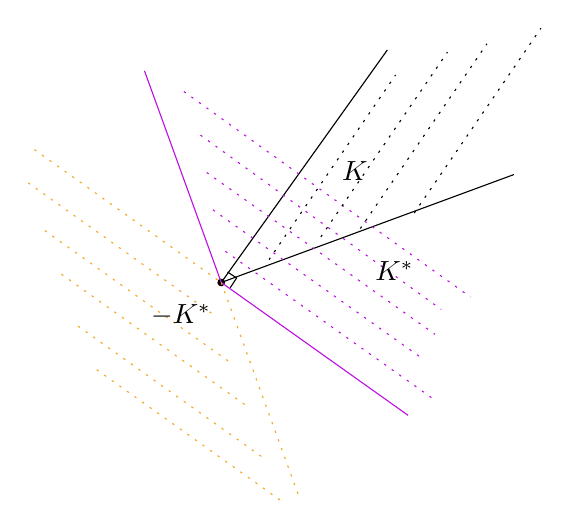
\begin{tikzpicture}[x=0.75pt,y=0.75pt,yscale=-1,xscale=1]
%uncomment if require: \path (0,300); %set diagram left start at 0, and has height of 300

%Straight Lines [id:da6369967985372562] 
\draw    (372,44) -- (292,156) ;
\draw [shift={(292,156)}, rotate = 125.54] [color={rgb, 255:red, 0; green, 0; blue, 0 }  ][fill={rgb, 255:red, 0; green, 0; blue, 0 }  ][line width=0.75]      (0, 0) circle [x radius= 1.34, y radius= 1.34]   ;
%Straight Lines [id:da8427154382623803] 
\draw    (433,104) -- (292,156) ;
%Straight Lines [id:da31509574892336034] 
\draw [color={rgb, 255:red, 189; green, 16; blue, 224 }  ,draw opacity=1 ]   (255,54) -- (292,156) ;
%Straight Lines [id:da2157097785076003] 
\draw [color={rgb, 255:red, 189; green, 16; blue, 224 }  ,draw opacity=1 ]   (292,156) -- (382,220) ;
%Shape: Right Angle [id:dp13367511075868022] 
\draw   (295.02,150.95) -- (299.4,153.8) -- (296.3,158.58) ;
%Straight Lines [id:da487766961447089] 
\draw [color={rgb, 255:red, 245; green, 166; blue, 35 }  ,draw opacity=1 ] [dash pattern={on 0.84pt off 2.51pt}]  (292,156) -- (329,258) ;
%Straight Lines [id:da573509136459132] 
\draw [color={rgb, 255:red, 245; green, 166; blue, 35 }  ,draw opacity=1 ] [dash pattern={on 0.84pt off 2.51pt}]  (202,92) -- (292,156) ;
%Straight Lines [id:da5379710009449119] 
\draw [color={rgb, 255:red, 245; green, 166; blue, 35 }  ,draw opacity=1 ] [dash pattern={on 0.84pt off 2.51pt}]  (215,152) -- (305,216) ;
%Straight Lines [id:da9818804420753207] 
\draw [color={rgb, 255:red, 245; green, 166; blue, 35 }  ,draw opacity=1 ] [dash pattern={on 0.84pt off 2.51pt}]  (207,131) -- (297,195) ;
%Straight Lines [id:da6021422350204104] 
\draw [color={rgb, 255:red, 245; green, 166; blue, 35 }  ,draw opacity=1 ] [dash pattern={on 0.84pt off 2.51pt}]  (199,108) -- (289,172) ;
%Straight Lines [id:da986013150105026] 
\draw [color={rgb, 255:red, 245; green, 166; blue, 35 }  ,draw opacity=1 ] [dash pattern={on 0.84pt off 2.51pt}]  (223,177) -- (313,241) ;
%Straight Lines [id:da6822452452629306] 
\draw [color={rgb, 255:red, 245; green, 166; blue, 35 }  ,draw opacity=1 ] [dash pattern={on 0.84pt off 2.51pt}]  (232,198) -- (322,262) ;
%Straight Lines [id:da17737739315026602] 
\draw [color={rgb, 255:red, 189; green, 16; blue, 224 }  ,draw opacity=1 ] [dash pattern={on 0.84pt off 2.51pt}]  (294,141) -- (394,212) ;
%Straight Lines [id:da83611836284918] 
\draw [color={rgb, 255:red, 189; green, 16; blue, 224 }  ,draw opacity=1 ] [dash pattern={on 0.84pt off 2.51pt}]  (288,121) -- (388,192) ;
%Straight Lines [id:da538992185351149] 
\draw [color={rgb, 255:red, 189; green, 16; blue, 224 }  ,draw opacity=1 ] [dash pattern={on 0.84pt off 2.51pt}]  (285,103) -- (395,181) ;
%Straight Lines [id:da10162860569722465] 
\draw [color={rgb, 255:red, 189; green, 16; blue, 224 }  ,draw opacity=1 ] [dash pattern={on 0.84pt off 2.51pt}]  (282,85) -- (398,169) ;
%Straight Lines [id:da257748503630693] 
\draw [color={rgb, 255:red, 189; green, 16; blue, 224 }  ,draw opacity=1 ] [dash pattern={on 0.84pt off 2.51pt}]  (274,64) -- (412,163) ;
%Straight Lines [id:da9128583904298737] 
\draw  [dash pattern={on 0.84pt off 2.51pt}]  (315,145) -- (376,56) ;
%Straight Lines [id:da9462720214604328] 
\draw  [dash pattern={on 0.84pt off 2.51pt}]  (340,134) -- (401,45) ;
%Straight Lines [id:da6400746610944403] 
\draw  [dash pattern={on 0.84pt off 2.51pt}]  (359,130) -- (420,41) ;
%Straight Lines [id:da14248692936540341] 
\draw  [dash pattern={on 0.84pt off 2.51pt}]  (385,122.5) -- (446,33.5) ;

% Text Node
\draw (349,96.4) node [anchor=north west][inner sep=0.75pt]    {$K$};
% Text Node
\draw (365,144.4) node [anchor=north west][inner sep=0.75pt]    {$K^{*}$};
% Text Node
\draw (257,165.4) node [anchor=north west][inner sep=0.75pt]    {$-K^{*}$};


\end{tikzpicture}


\caption{Visualization of the dual cone. (Note in some books, $-K^{*}$ is defined as the dual cone.)}\label{fig:conx_proo3}
\end{figure}
\begin{rema}
As the name suggests, $K^{*}$ is always a convex cone, even when the original cone $K$ is just a conic but not convex.
\end{rema}
\begin{exma}{\bfs{subspace}}
 The dual cone of a subspace $V \subseteq \mathbf{R}^{n}$ (which is a cone) is its orthogonal complement $V^{\perp}=\left\{y \mid v^{\top} y=0\right.$ for all $\left.v \in \bar{V}\right\}$. The equality is because $-y\in M$ if $y\in V$.
\end{exma}
\begin{exma}{\bfs{nonnegative orthant}}
  The cone $\mathbf{R}_{+}^{n}$ is its own dual:
\begin{align*}
y^{\top} x \geq 0 \text { for all } x \succeq 0 \Longleftrightarrow y \succeq 0
\end{align*}
We call such a cone \tb{self-dual}.
\end{exma}
\begin{exma}{\bfs{positive semidefinite cone}}\label{exm:sem_con}
   On the set of symmetric $n \times n$ matrices $\mathbf{S}^{n}$, we use the standard inner product $\operatorname{tr}(X Y)=\sum_{i, j=1}^{n} X_{i j} Y_{i j}$. The positive semidefinite cone $\mathbf{S}_{+}^{n}$ is self-dual, i.e., for $X, Y \in \mathbf{S}^{n}$
\begin{align*}
\operatorname{tr}(X Y) \geq 0 \text { for all } X \succeq 0 \Longleftrightarrow Y \succeq 0
\end{align*}
We will show this fact:

``$\Rightarrow$'': Suppose $Y \notin \mathbf{S}_{+}^{n} .$ Then there exists $q \in \mathbf{R}^{n}$ with
\begin{align*}
q^{\top} Y q=\operatorname{tr}\left(q q^{\top} Y\right)<0
\end{align*}
Hence the positive semidefinite matrix $X=q q^{\top}$ satisfies $\operatorname{tr}(X Y)<0$; it follows that $Y \notin\left(\mathbf{S}_{+}^{n}\right)^{*}$.

``$\Leftarrow$'': Now suppose $X, Y \in \mathbf{S}_{+}^{n} .$ We can express $X$ in terms of its eigenvalue decomposition as $X=\sum_{i=1}^{n} \lambda_{i} q_{i} q_{i}^{\top}$, where (the eigenvalues) $\lambda_{i} \geq 0, i=1, \ldots, n$. Then we have
\begin{align*}
\operatorname{tr}(Y X)=\operatorname{tr}\left(Y \sum_{i=1}^{n} \lambda_{i} q_{i} q_{i}^{\top}\right)=\sum_{i=1}^{n} \lambda_{i} q_{i}^{\top} Y q_{i} \geq 0
\end{align*}
This shows that $Y \in\left(\mathbf{S}_{+}^{n}\right)^{*}$.
\end{exma}
\begin{exma}{\bfs{dual of a norm cone}}
  Let $\|\cdot\|$ be a norm on $\mathbf{R}^{n}$. The dual of the associated cone $K=\left\{(x, t) \in \mathbf{R}^{n+1} \mid\|x\| \leq t\right\}$ is the \tb{cone defined by the dual norm}, i.e.,
\begin{align*}
K^{*}=\left\{(u, v) \in \mathbf{R}^{n+1} \mid\|u\|_{*} \leq v\right\}
\end{align*} 
where the \tb{dual norm} is given by $\|u\|_{*}=\sup \left\{u^{\top} x \mid\|x\| \leq 1\right\}$ (see \cite[P326]{horn2012matrix}).

To prove the result we have to show that
\begin{align*}
x^{\top} u+t v \geq 0 \text { whenever }\|x\| \leq t \Longleftrightarrow\|u\|_{*} \leq v
\end{align*}

``$\Leftarrow$'': Suppose $\|u\|_{*} \leq v$, and $\|x\| \leq t$ for some $t>0$. (If $t=0, x$ must be zero, so obviously $u^{\top} x+v t \geq 0$.) Applying the definition of the dual norm, and the fact that $\|-x / t\| \leq 1$, we have
\begin{align*}
u^{\top}(-x / t) \leq\|u\|_{*} \leq v
\end{align*}
and therefore $u^{\top} x+v t \geq 0$

``$\Rightarrow$'': Suppose $\|u\|_{*}>v$, i.e., that the righthand condition does not hold. Then by the definition of the dual norm, there exists an $x$ with $\|x\| \leq 1$ and $x^{\top} u>v$ Taking $t=1$, we have
\begin{align*}
u^{\top}(-x)+v<0
\end{align*}
which contradicts the lefthand condition.
\end{exma}

\paragraph{Properties of Dual Cones}\label{sec:pr_du_con}
\begin{enumerate}
    \item \tb{$K^{*}$ is closed and convex:}
    
    ($K^*$ is the intersection of a set of halfspaces)
    \item \tb{$K_{1} \subseteq K_{2}$ implies $K_{2}^{*} \subseteq K_{1}^{*}$.}
    \item  \tb{If $K$ has nonempty interior, then $K^{*}$ is pointed:}
        
        (assume $K^{*}$ is not pointed, it contains lines, i.e. $\exists x\ne 0$ s.t. $x \in K^{*}$ and $-x \in K^{*}$. For any $y\in K$ we have $x^{\top}y\ge 0$ and $-x^{\top}y\ge 0$. Therefore $x^{\top}y= 0$ for all $y\in K$. Note since $K$ has nonempty interior, $\Aff (K)$ is the full space. This is not possible for  $x^{\top}y= 0$ with $x\ne 0$.)
    \item \tb{If the closure of convex cone $K$ is pointed then $K^{*}$ has nonempty interior:}
    
        (assume  $K^{*}$ has empty interior,  $\Aff (K^{*})$ then has dimension $<n$: with possible translate, we have $\Aff (K^{*})$ is the nullspace $H\coloneqq\{x: Ax=0\}$, and of course $K^{*}\subseteq H$. Then $\operatorname{range}A=H^*\subseteq K^{**}=\cl \Conv(K)$ which is not pointed.)
    \item \tb{$\inte K^{*}=\left\{y \mid y^{\top} x>0\text{ for all }x \in K, x\ne 0\right\}$}:
    
 (``$\supset$'': Let $H=\{x\mid ||x||=1,x \in K\}$.  $y^{\top} x>0,\forall x \in K$ $\Rightarrow$ $y^{\top} x>0,\forall x\in H$ $\Rightarrow$ $(y+u)^{\top} x>0$ for all $x \in H$ and all sufficiently small $||u||<\delta$ $\Rightarrow$ $(y+u)^{\top} x>0,\forall x\in K$ and all sufficiently small $||u||<\delta$ $\Rightarrow$ $y \in \inte K^*$.
 
``$\subset$'':  if $y \in K^{*}$ and $y^{\top} x=0$ for some $x \in K$, then $y \notin$ int $K^{*}$ because $(y-t x)^{\top} x<0$ for all $t>0$.)
    \item \tb{$K^{* *}$ is the closure of the convex hull of $K$;}
    
    Hence \tb{if $K$ is convex and closed, $K^{* *}=K$:}
    
    (WLOG, assume $K$ is convex. $y \neq 0$ is the normal vector of a (homogeneous) halfspace containing $K$ if and only if $y \in K^{*}$. The intersection of all homogeneous halfspaces containing a convex cone $K$ is the closure of $K .$ Therefore the closure of $K$ is
\begin{align*}
\operatorname{cl} K=\bigcap_{y \in K^{*}}\left\{x \mid y^{\top} x \geq 0\right\}=\left\{x \mid y^{\top} x \geq 0 \text { for all } y \in K^{*}\right\}=K^{* *}
\end{align*})
 
    
\item \tb{If $K$ is a \tb{proper cone, then so is its dual $K^{*}$}, and moreover, that $K^{* *}=K$}
\end{enumerate}



\subsubsection{Dual Generalized Inequalities}
Now suppose that the convex cone $K$ is proper, so it induces a generalized inequality $\preceq_{K} .$ Then its dual cone $K^{*}$ is also proper, and therefore induces a generalized inequality. We refer to the generalized inequality $\preceq_{K^{*}}$ as the dual of the generalized inequality $\preceq_{K}$.

\paragraph{Properties of Generalized Inequality and Dual}
\begin{enumerate}
    \item \tb{$x \preceq_{K} y$ if and only if $\lambda^{\top} x \leq \lambda^{\top} y$ for all $\lambda \succeq_{K^{*}} 0$:}
    
    ($K^{**}=K$, so $y-x\in K$ $\Longleftrightarrow$ $y-x\in K^{**}$ $\Longleftrightarrow$ $\lambda^{\top}(y-x)\ge 0, \forall \lambda \in K^*$)
    \item \tb{$x \prec_{K} y$ if and only if $\lambda^{\top} x<\lambda^{\top} y$ for all $\lambda \succeq_{K^{*}} 0, \lambda \neq 0$:}
    
    (``$\Rightarrow$'':  from 1, if $\lambda^{\top}(y-x)=0$, we have $\lambda =0$ since $y-x\in \inte K$; 
    
    ``$\Leftarrow$'': this is a restatement of Properties of Dual Cones 5.)
    
    
\end{enumerate}
\begin{rema}
Since $K=K^{* *}$, the dual generalized inequality associated with $\preceq_{K^{*}}$ is $\preceq_{K}$, so these properties hold if the generalized inequality and its dual are swapped.
\end{rema}

\begin{thma}{\bfs{alternatives for linear strict generalized inequalities}}\label{exm:fafdavcz}\label{eq:yrrew}
 Suppose $K \subseteq \mathbf{R}^{m}$ is a proper cone. Consider the strict generalized inequality
\begin{align}
A x \prec_{K} b\label{eq:bvtu}
\end{align}
where $x \in \mathbf{R}^{n}$. Consider also
\begin{align}
\exists \lambda\in \mathbf{R}^m \text{ s.t } \lambda \neq 0, \quad \lambda \succeq_{K^{*}} 0, \quad A^{\top} \lambda=0, \quad \lambda^{\top} b \leq 0 \label{eq:vbc}
\end{align}
We have 

``\centerline{\cref{eq:vbc} is  \tb{feasible} ''$\Longleftrightarrow$ ``\cref{eq:bvtu} is \tb{infeasible}''}

\end{thma}

\begin{proof}\color{ForestGreen}
``$\Leftarrow$'':

Suppose \cref{eq:vbc} is infeasible, i.e., the affine set $\left\{b-A x \mid x \in \mathbf{R}^{n}\right\}$ does not intersect the open convex set $\operatorname{int} K$. Then there is a separating hyperplane, i.e., a nonzero $\lambda \in \mathbf{R}^{m}$ and $\mu \in \mathbf{R}$ such that $\lambda^{\top}(b-A x) \leq \mu$ for all $x$, and $\lambda^{\top} y \geq \mu$ for all $y \in\inte K$. The first condition implies $A^{\top} \lambda=0$ and $\lambda^{\top} b \leq \mu .$ The second condition implies $\lambda^{\top} y \geq \mu$ for all $y \in K$, which can only happen if $\lambda \in K^{*}$ and $\mu \leq 0$.
Putting it all together we get \cref{eq:vbc}.

``$\Rightarrow$'':

Suppose that both inequality systems hold. Then we have $\lambda^{\top}(b-A x)>$ 0, since $\lambda \neq 0, \lambda \succeq_{K^{*}} 0$, and $b-A x \succ_{K} 0 .$ But using $A^{\top} \lambda=0$ we find that $\lambda^{\top}(b-A x)=\lambda^{\top} b \leq 0$, which is a contradiction.

\end{proof}

\begin{rema}\tb{strong alternatives}
Thus, the inequality systems \cref{eq:bvtu} and \cref{eq:vbc} are alternatives: for any data $A, b$, \tb{exactly one of them is feasible}. This generalizes the alternatives \cref{exm:mnm,exm:mnm1} for the special case $K=\mathbf{R}_{+}^{m}$.

This is quite similar to Farkas Lemma (see \cref{cora:gene_fark}). Please compare.  We state the general methodology in \cref{sec:bmqdfd} called \tb{strong alternatives}.
\end{rema}
  
\paragraph{Minimum and Minimal Elements via Dual Inequalities}\label{sec:yiiue}
We can use \tb{dual generalized inequalities} to characterize minimum and minimal elements of a (possibly nonconvex) set $S \subseteq \mathbf{R}^{m}$ with respect to the generalized inequality induced by a proper cone $K$.

\tb{$\bullet$ dual characterization of minimum element}
\begin{lema}
  ``$x$ is the \tb{minimum} element of $S$, w.r.t $\preceq_{K}$''$\Longleftrightarrow$  ``\tb{for all} $\lambda \succ_{K^{*}} 0, x$ is the unique minimizer of $\lambda^{\top} z$ over $z \in S$'' 
\end{lema}
\begin{rema}{\bfs{explanation}}
Geometrically, this means that for any $\lambda \succ_{K^{*}} 0$, the hyperplane
\begin{align*}
\left\{z \mid \lambda^{\top}(z-x)=0\right\}
\end{align*}
is a strict supporting hyperplane to $S$ at $x .$ (By strict supporting hyperplane, we mean that the hyperplane intersects $S$ only at the point $x .$ ) Note that convexity of the set $S$ is not required.  See \cref{fig:duan_mini} for better understanding.
\end{rema}
\begin{figure}
    \centering
    \includegraphics[width=0.5\textwidth]{Figs/1.png}
    \caption{Dual of minimum: $x$ is minimum element of the set $S$ w.r.t $\mathbf{R}_{+}^{2}$; for every $\lambda \succ 0$, the hyperplane $\left\{z \mid \lambda^{\top}(z-x)=0\right\}$ strictly supports $S$ at $x$, i.e., contains $S$ on one side, and touches it only at $x$.}
    \label{fig:duan_mini}
\end{figure}
\begin{figure}
    \centering
    \includegraphics[width=0.4\textwidth]{Figs/7.png}
    \caption{ The point $x_{1} \in S_{1}$ is minimal, but is not a minimizer of $\lambda^{\top} z$ over $S_{1}$ for any $\lambda \succ 0$. (It does, however, minimize $\lambda^{\top} z$ over $z \in S_{1}$ for $\lambda=(1,0) .$ Right. The point $x_{2} \in S_{2}$ is not minimal, but it does minimize $\lambda^{\top} z$ over $z \in S_{2}$ for $\lambda=(0,1) \succeq 0$}
    \label{fig:duan_mini_safd}
\end{figure}
\begin{proof}\color{ForestGreen}
``$\Rightarrow$'': suppose $x$ is the minimum element of $S$, i.e., $x \preceq_{K} z$ for all $z \in S$, and let $\lambda \succ_{K^{*}} 0 .$ Let $z \in S, z \neq x$, we have $z-x \succeq_{K} 0 .$ From $\lambda \succ_{K^{*}} 0$ and $z-x \succeq_{K} 0, z-x \neq 0$, we conclude $\lambda^{\top}(z-x)>0$. Since $z$ is an arbitrary element of $S$, not equal to $x$, this shows that $x$ is the unique minimizer of $\lambda^{\top} z$ over $z \in S$. 

``$\Leftarrow$'': suppose that for all $\lambda \succ_{K^{*}} 0, x$ is the unique minimizer of $\lambda^{\top} z$ over $z \in S$, but $x$ is not the minimum element of $S$. Then there exists $z \in S$ with $z \nsucceq_{K} x$. Since $z-x \nsucceq_{K} 0$, there exists $\tilde{\lambda} \succeq_{K}^{*} 0$ with $\tilde{\lambda}^{\top}(z-x)<0 .$ Hence $\lambda^{\top}(z-x)<0$ for $\lambda \succ_{K^{*}} 0$ in the neighborhood of $\tilde{\lambda}$. This contradicts the assumption that $x$ is the unique minimizer of $\lambda^{\top} z$ over $S$.
\end{proof}

\tb{$\bullet$ dual characterization of minimal element}

\begin{lema}{\bfs{sufficiency}}\label{lem:ss}
  If $\exists \lambda \succ_{K^{*}} 0$ and $x$ minimizes $\lambda^{\top} z$ over $z \in S$, then $x$ is minimal. 
\end{lema}
\begin{rema}
This is illustrated in \cref{fig:duan_mini_s}. Please note $\succ_{K^{*}}$ cannot be replaced by $\succeq_{K^{*}}$. See \cref{fig:duan_mini_safd}
\end{rema}
\begin{figure}[H]
    \centering
    \includegraphics[width=0.4\textwidth]{Figs/2.png}
    \caption{A set $S \subseteq \mathbf{R}^{2}$. Its set of minimal points, w.r.t $\mathbf{R}_{+}^{2}$, is shown as the darker section of its (lower, left) boundary. The minimizer of $\lambda_{1}^{\top} z$ over $S$ is $x_{1}$, and is minimal since $\lambda_{1} \succ 0 .$ The minimizer of $\lambda_{2}^{\top} z$ over $S$ is $x_{2}$, which is another minimal point of $S$, since $\lambda_{2} \succ 0$}
    \label{fig:duan_mini_s}
\end{figure}
\begin{proof}\color{ForestGreen}
Suppose that $\lambda \succ_{K^{*}} 0$, and $x$ minimizes $\lambda^{\top} z$ over $S$, but $x$ is not minimal, i.e., there exists a $z \in S, z \neq x$, and $z \preceq_{K} x$. Then $\lambda^{\top}(x-z)>0$, which contradicts our assumption that $x$ is the minimizer of $\lambda^{\top} z$ over $S$.
\end{proof} 
However, the converse is in general false: a point $x$ can be minimal in $S$, but not a minimizer of $\lambda^{\top} z$ over $z \in S$, for any $\lambda$, as shown in \cref{fig:duan_mini_nf}.  We need \tb{convexity}.
\begin{figure}
    \centering
    \includegraphics[width=0.4\textwidth]{Figs/3.png}
    \caption{The point $x$ is a minimal element of $S \subseteq \mathbf{R}^{2}$ with respect to $\mathbf{R}_{+}^{2} .$ However there exists no $\lambda$ for which $x$ minimizes $\lambda^{\top} z$ over $z \in S$.}
    \label{fig:duan_mini_nf}
\end{figure}
\begin{lema}{\bfs{necessity}}\label{lem:ghfito}
  Provided the set $S$ is convex, we can say that \tb{for any} minimal element $x$ there exists a nonzero $\lambda \succeq_{K^{*}} 0$ such that $x$ minimizes $\lambda^{\top} z$ over $z \in S$.
\end{lema}
\begin{rema}
Please note $\succeq_{K^{*}}$ cannot be replaced by $\succ_{K^{*}}$. See \cref{fig:duan_mini_safd}.
\end{rema}
\begin{proof}\color{ForestGreen}
Suppose $x$ is minimal, which means that $((x-K) \backslash\{x\}) \cap S=\emptyset$. Applying the separating hyperplane theorem to the convex sets $(x-K) \backslash\{x\}$ and $S$, we conclude that there is a $\lambda \neq 0$ and $\mu$ such that $\lambda^{\top}(x-y) \leq \mu$ for all $y \in K$ and $\lambda^{\top} z \geq \mu$ for all $z \in S$. From the first inequality we conclude $\lambda \succeq_{K^{*}} 0$. Since $x \in S$ and $x \in x-K$, we have $\lambda^{\top} x=\mu$, so the second inequality implies that $\mu$ is the minimum value of $\lambda^{\top} z$ over $S .$ Therefore, $x$ is a minimizer of $\lambda^{\top} z$ over $S$ where $\lambda \neq 0, \lambda \succeq_{K^{*}} 0$
\end{proof} 


\begin{exma}{\bfs{Pareto optimal production frontier}}
   With each production method, we associate a resource vector $x \in \mathbf{R}^{n}$, where $x_{i}$ denotes the amount of resource $i$ consumed by the method to manufacture the product. Pareto optimal is the minimal.

We can find Pareto optimal production methods (i.e., minimal resource vectors) by minimizing
\begin{align*}
\lambda^{\top} x=\lambda_{1} x_{1}+\cdots+\lambda_{n} x_{n}
\end{align*}
over the set $P$ of production vectors, using any $\lambda$ that satisfies $\lambda \succ 0$. However we this is the \tb{sufficient condition} shown in \cref{lem:ss} and \tb{cannot guarantee} we can find all Pareto optimal. See \cref{fig:duan_mini_nfbgf}.
\begin{figure}[H]
    \centering
    \includegraphics[width=0.4\textwidth]{Figs/5.png}
    \caption{The production set $P$, for a product that requires labor and fuel to produce, is shown shaded. The two dark curves show the efficient production frontier. The points $x_{1}, x_{2}$ and $x_{3}$ are efficient. The points $x_{4}$ and $x_{5}$ are not (since in particular, $x_{2}$ corresponds to a production method that uses no more fuel, and less labor). The point $x_{1}$ is also the minimum cost production method for the price vector $\lambda$ (which is positive). The point $x_{2}$ is efficient, but \tb{cannot be found by minimizing} the total $\operatorname{cost} \lambda^{\top} x$ for any price vector $\lambda \succeq 0$.}
    \label{fig:duan_mini_nfbgf}
\end{figure}
\end{exma}

\section{Convex Function}\label{sec:conx_f}
\subsection{Basic Definitions and Examples}
\begin{defa}{\bfs{Convex Function}}
  A function $f: M \rightarrow \mathbf{R}$ defined on a nonempty subset $M$ of $\mathbf{R}^{n}$ and taking real values is called \tb{convex}, if
\begin{itemize}
    \item the domain $M$ of the function is \tb{convex};
    \item it satisfies \begin{align}\vspace{-0.4cm}\begin{aligned}
      f(\lambda x+(1-\lambda) y) \le \lambda f(x)+(1-\lambda) f(y), \quad x, y \in M, \lambda \in[0,1]\label{eq:con_f}
      \end{aligned}
\end{align}
\end{itemize}
If the above inequality is strict whenever $x \neq y$ and $0<\lambda<1, f$ is called \tb{strictly convex}.
\end{defa}
\begin{figure}[H]
\centering


\tikzset{every picture/.style={line width=0.75pt}} %set default line width to 0.75pt        

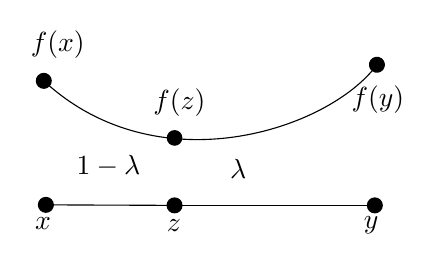
\begin{tikzpicture}[x=0.75pt,y=0.75pt,yscale=-1,xscale=1]
%uncomment if require: \path (0,300); %set diagram left start at 0, and has height of 300

%Straight Lines [id:da1885857134189366] 
\draw    (70.5,140.5) -- (132.5,140.75) ;
\draw [shift={(132.5,140.75)}, rotate = 0.23] [color={rgb, 255:red, 0; green, 0; blue, 0 }  ][fill={rgb, 255:red, 0; green, 0; blue, 0 }  ][line width=0.75]      (0, 0) circle [x radius= 3.35, y radius= 3.35]   ;
\draw [shift={(70.5,140.5)}, rotate = 0.23] [color={rgb, 255:red, 0; green, 0; blue, 0 }  ][fill={rgb, 255:red, 0; green, 0; blue, 0 }  ][line width=0.75]      (0, 0) circle [x radius= 3.35, y radius= 3.35]   ;
%Straight Lines [id:da5566947758965337] 
\draw    (132.5,140.75) -- (229,140.75) ;
\draw [shift={(229,140.75)}, rotate = 0] [color={rgb, 255:red, 0; green, 0; blue, 0 }  ][fill={rgb, 255:red, 0; green, 0; blue, 0 }  ][line width=0.75]      (0, 0) circle [x radius= 3.35, y radius= 3.35]   ;
%Curve Lines [id:da2140869189476351] 
\draw    (69.5,80.75) .. controls (124.5,131.75) and (207,104.25) .. (230,73) ;
\draw [shift={(230,73)}, rotate = 306.35] [color={rgb, 255:red, 0; green, 0; blue, 0 }  ][fill={rgb, 255:red, 0; green, 0; blue, 0 }  ][line width=0.75]      (0, 0) circle [x radius= 3.35, y radius= 3.35]   ;
\draw [shift={(69.5,80.75)}, rotate = 42.84] [color={rgb, 255:red, 0; green, 0; blue, 0 }  ][fill={rgb, 255:red, 0; green, 0; blue, 0 }  ][line width=0.75]      (0, 0) circle [x radius= 3.35, y radius= 3.35]   ;
%Shape: Ellipse [id:dp38592273618409423] 
\draw  [fill={rgb, 255:red, 0; green, 0; blue, 0 }  ,fill opacity=1 ] (129,108.25) .. controls (129,106.32) and (130.57,104.75) .. (132.5,104.75) .. controls (134.43,104.75) and (136,106.32) .. (136,108.25) .. controls (136,110.18) and (134.43,111.75) .. (132.5,111.75) .. controls (130.57,111.75) and (129,110.18) .. (129,108.25) -- cycle ;

% Text Node
\draw (64,145.4) node [anchor=north west][inner sep=0.75pt]    {$x$};
% Text Node
\draw (222.5,144.9) node [anchor=north west][inner sep=0.75pt]    {$y$};
% Text Node
\draw (127.5,146.4) node [anchor=north west][inner sep=0.75pt]    {$z$};
% Text Node
\draw (62,55.4) node [anchor=north west][inner sep=0.75pt]    {$f( x)$};
% Text Node
\draw (121,83.4) node [anchor=north west][inner sep=0.75pt]    {$f( z)$};
% Text Node
\draw (216.5,81.9) node [anchor=north west][inner sep=0.75pt]    {$f( y)$};
% Text Node
\draw (84,115.4) node [anchor=north west][inner sep=0.75pt]    {$1-\lambda $};
% Text Node
\draw (158,117.4) node [anchor=north west][inner sep=0.75pt]    {$\lambda $};


\end{tikzpicture}

\caption{Visualization of convex function.}\label{fig:conx_ff}
\end{figure}
\begin{rema}{\bfs{alternative form I}}\label{rem:albc} With $z=y+\lambda(x- y)$
\cref{eq:con_f} sometimes is written as 
\begin{align}\begin{aligned}
      f(z) \le  f(y)+\lambda \left(f(x)-f(y)\right), \quad x, y \in M, \lambda \in[0,1]\label{eq:con_ff}
      \end{aligned}
\end{align}
or
\begin{align}\begin{aligned}
      f(z)-  f(y)\le \lambda \left(f(x)-f(y)\right), \quad x, y \in M, \lambda \in[0,1]\label{eq:con_ff1}
      \end{aligned}
\end{align}

\end{rema}
\begin{rema}{\bfs{alternative form II of univariate $f$}}\label{rem:alc}
In $\mathbf{R}$ space,  $f$ is defined in $(a,b)$, for \tb{any} three variable $a<x<z<y<b$, we have $z=x\frac{y-z}{y-x}+y\frac{z-x}{y-x}$. We sometimes write the convexity as follows:
\begin{align*}
    f(z)\le \frac{y-z}{y-x}f(x)+\frac{z-x}{y-x}f(y),\forall a<x<z<y<b\Longleftrightarrow f\text{ is convex on } (a,b)
\end{align*}
Equivalently we have 
\begin{align}
 f(z)-f(x)\le \frac{z-x}{y-x}(f(y)-f(x)) ,\forall a<x<z<y<b&\Longleftrightarrow f\text{ is convex on } (a,b)\label{eq:real_conx}
 \end{align}
 Or more generally, $\forall a<x<z<y<b$,
 \begin{align}
    \text{\tb{any two of }}  \frac{f(z)-f(x)}{z-x}\le \frac{f(y)-f(x)}{y-x}\le \frac{f(y)-f(z)}{y-z} \Longleftrightarrow f\text{ is convex on } (a,b)\label{eq:real_conx2}
\end{align}
See also \cref{thm:ccuf} for the nondecreasing property of $f'$.
\end{rema}
\begin{rema}{\bfs{alternative form III}}\label{rem:alccc}
Note, for general multivariate $f$, we can write $\|x-y\|_2$ instead of $x-y$, i.e.
\begin{align}
 f(z)-f(x)\le \frac{\|z-x\|_2}{\|y-x\|_2}(f(y)-f(x)) ,\forall x,z,y \text{ collinear with $z$ inside $[x,y]$}  &\Longleftrightarrow f\text{ is convex on } (a,b)\label{eq:real_conx3}
 \end{align}

\end{rema}
\begin{defa}{\bfs{Concave Function}}
  A function $f$ such that $-f$ is convex is called \tb{concave}:
  \begin{itemize}
      \item the domain $M$ of the function is \tb{convex};
      \item it satisfies \begin{align*}\vspace{-0.4cm}\begin{aligned}
      f(\lambda x+(1-\lambda) y) \geq \lambda f(x)+(1-\lambda) f(y), \quad x, y \in M, \lambda \in[0,1]
      \end{aligned}
\end{align*}
  \end{itemize} 
\end{defa}
\begin{exma}{\bfs{affine is convex and concave}}
   The simplest example of a convex function is an affine function
\begin{align*}
f(x)=a^{\top} x+b
\end{align*}
\tb{\centerline{$f$ both convex and concave on the entire space $\Longleftrightarrow$ $f$ is an affine function.}}
\end{exma}
\begin{thma}{\bfs{every norm is convex}}
 Let $\pi(x)$ be a real-valued function on $\mathbf{R}^{n}$ which is positively homogeneous of degree 1 :
\begin{align*}
\pi(t x)=t \pi(x) \quad \forall x \in \mathbf{R}^{n}, t \geq 0
\end{align*}
$\pi$ is convex if and only if it is sub-additive:
\begin{align*}
\pi(x+y) \leq \pi(x)+\pi(y) \quad \forall x, y \in \mathbf{R}^{n}
\end{align*}
In particular, a norm (which by definition is positively homogeneous of degree 1 and is subadditive) is convex.
\end{thma}
\begin{proof}\color{ForestGreen}
\begin{align*}
\begin{aligned}
\pi(\lambda x+(1-\lambda) y) & \leq \pi(\lambda x)+\pi((1-\lambda) y) & \text { triangle inequality } \\
&=\lambda \pi(x)+(1-\lambda) \pi(y) & \text { homogeneity }
\end{aligned}
\end{align*}
for any $x, y \in \mathbf{R}^{n}$ and $0 \leq \lambda \leq 1$.
\end{proof}
\subsubsection{Some Equivalent Convexity Form}
\begin{thma}{\bfs{equivalent condition for convex: I}} \label{thm:conx2onev}

\tb{\centerline{$f$ is convex $\Longleftrightarrow$  $g(t)=f(x+t h)$ is convex  $\forall x\in \dom f$ and $h$}}
\end{thma}
\begin{rema}
This property is very useful, since it allows us to check whether a function is convex by restricting it to a line. Here I mean $g(t)$ is convex on its domain: $\{t \mid x+t v \in \dom  f\}$.  
\end{rema}
\begin{rema}
It is a speical case of ``Composition with Affine Mapping'' as shown in \cref{sec:oper_conv}.
\end{rema}
\begin{proof}\color{ForestGreen}
``$\Rightarrow$'':
It is clear that $\dom g$ is convex. For any $t_1,t_2\in \dom g$
\begin{align*}
    g(\lambda t_1 + (1-\lambda) t_2)&=f(x+ (\lambda t_1 + (1-\lambda) t_2)h))\\
    &=f(\lambda(t_1h+x)+ (1-\lambda)(t_2h+x))\\
    &\le \lambda g(t_1)+(1-\lambda)g(t_2)
\end{align*}

``$\Leftarrow$'': 
If $g$ is convex for any $x$ and $h$. For any $x,y\in \dom f$, let $h=y-x$.  We get convexity of $f$.
\end{proof}
\begin{defa}{\bfs{Epigraph}}
 Given a real-valued function $f$ defined on a nonempty subset $M$ of $\mathbf{R}^{n}$, we define its \tb{epigraph} as the set
\begin{align}
\Epi (f)=\left\{(t, x) \in \mathbf{R}^{n+1} \mid x \in M, t \geq f(x)\right\}\label{eq:epi_f}
\end{align}
\end{defa}
\begin{thma}{\bfs{equivalent condition for convex: II}} 

\tb{\centerline{$f$ defined on $M\subseteq \mathbf{R}^n$ is convex $\Longleftrightarrow$ $\Epi (f)$ is a nonempty convex set in $\mathbf{R}^{n+1}$.}}
\end{thma}
\begin{rema}\bfs{what is a convex epigrah}\label{rem:epi_cfa}
$\Epi (f)$ is \tb{not} an arbitrary convex set in $\mathbf{R}^{n+1}$. It must contains one \tb{recessive direction} $(1,0)$, $0\in \mathbf{R}^n$, see \cref{def:recessive_dir}. Conversely, for any convex set with one recessive direction, by possible rotation (coordinate transform), we may define a convex function with its epigraph being the convex set.
\end{rema}
\begin{proof}\color{ForestGreen}
``$\Rightarrow$'': Since $f$ is convex we have $\dom f$ is convex. Let $(t_1,x),(t_2,y)\in \Epi (f)$. $\lambda x + (1-\lambda) y\in \dom f$ and $f(\lambda x + (1-\lambda) y)\le \lambda f(x) + (1-\lambda)f(y)\le \lambda t_1 + (1-\lambda) t_2$. We then have $( \lambda t_1 + (1-\lambda) t_2, \lambda x + (1-\lambda) y)\in \Epi (f)$.

``$\Leftarrow$'': $\dom f$ is convex from the projection of $\Epi (f)$. $(f(x),x), (f(y),y) \in \Epi(f)\Leftarrow f(\lambda x + (1-\lambda) y)\le \lambda f(x) + (1-\lambda)f(y)$.
\end{proof}
\begin{exma}{\bfs{epigraph of matrix fractional function.}}
The function $f: \mathbf{R}^{n} \times \mathbf{S}^{n} \rightarrow \mathbf{R}$, defined as
\begin{align*}
f(x, Y)=x^{\top} Y^{-1} x
\end{align*}
is convex on $\dom  f=\mathbf{R}^{n} \times \mathbf{S}_{++}^{n}$. (This generalizes the quadratic-over-linear function $f(x, y)=x^{2} / y$, with $\left.\dom  f=\mathbf{R} \times \mathbf{R}_{++} \cdot\right)$
One easy way to establish convexity of $f$ is via its epigraph:
\begin{align*}
\begin{aligned}
\Epi (f) &=\left\{(x, Y, t) \mid Y \succ 0, x^{\top} Y^{-1} x \leq t\right\} \\
&=\left\{(x, Y, t) \mid\left[\begin{array}{cc}
Y & x \\
x^{\top} & t
\end{array}\right] \succeq 0, Y \succ 0\right\}
\end{aligned}
\end{align*}
using the Schur complement condition for positive semidefiniteness of a block matrix. The last condition is a linear matrix inequality in $(x, Y, t)$, and therefore  $\Epi (f)$ is convex.
\end{exma}
\begin{lema}{\bfs{Sufficient Convexity Condition for Continuous Function on Real Line}}
Assume that $f$ is a continuous real function defined in $(a, b)$ such that
\begin{align*}
f\left(\frac{x+y}{2}\right) \leq \frac{f(x)+f(y)}{2}
\end{align*}
for all $x, y \in(a, b) .$ Prove that $f$ is convex.
\end{lema}
\begin{proof}\color{ForestGreen}
See \cite[page 101, ex. 24]{rudin1976principles}
\end{proof}
\subsubsection{Sublevel Set}
\begin{defa}{\bfs{Sublevel Set}}
 Given a scalar $c \in \mathbb{R}$ and a function $f: \mathbb{R}^{n} \rightarrow \mathbb{R}$, a \tb{sublevel set} of $f$ associated with $c$ is given by
\begin{align}
L_{c}(f)=\{x \in \dom  f \mid f(x) \leq c\}\label{eq:sublev_f}
\end{align}
\end{defa}
\begin{rema}{\bfs{convex and sublevel set}}
Every level set of a convex function is convex: if $x, y \in L_{\alpha}(f)$ and $\lambda \in[0,1]$, then $f(\lambda x+(1-\lambda) y) \leq \lambda f(x)+$ $(1-\lambda) f(y) \leq \lambda \alpha+(1-\lambda) \alpha=\alpha$, so that $\lambda x+(1-\lambda) y \in L_{\alpha}(f)$

Converse is \tb{false}: consider $f(x)=-e^{x}$ for $x \in \mathbb{R}$.
\end{rema} 

\begin{exma}{\bfs{norm ball and ellipsoid}}\label{exm:ball_ell}
The unit ball of norm $\|\cdot\|$ - the set
\begin{align*}
\left\{x \in \mathbf{R}^{n} \mid\|x\| \leq 1\right\}
\end{align*}
same as any other $\|\cdot\|$-ball
\begin{align*}
\{x \mid\|x-a\| \leq r\}
\end{align*}
$\left(a \in \mathbf{R}^{n}\right.$ and $r \geq 0$ are fixed) is convex and closed (from continuity of $||\cdot||$).

One special example is the ellipsoid $\mathcal{E}=\left\{x \mid\left(x-x_{c}\right)^{\top} P^{-1}\left(x-x_{c}\right) \leq 1\right\}$ with positive definite $P$ is closed and norm because $||x||_P = \sqrt{x^{\top}Px}$ is also a norm.
\end{exma}
\begin{exma}{\bfs{$\epsilon$-neighborhood of a convex set}}\label{rem:dis_con_1}
Let $M$ be a convex set in $\mathbf{R}^{n}$, and let $\epsilon>0$. Then, for any norm $\|\cdot\|$ on $\mathbf{R}^{n}$, the $\epsilon$-neighborhood of $M$, i.e., the set
\begin{align*}
M_{\epsilon}=\left\{y \in \mathbf{R}^{n} \mid \operatorname{dist}_{\|\cdot\|}(y, M) \coloneqq \inf _{x \in M}\|y-x\| \leq \epsilon\right\}
\end{align*}
is convex and closed:

Note $\operatorname{dist}_{\|\cdot\|}(\cdot, M)$ is (uniform) continuous, closed is then clear. Note $ \operatorname{dist}_{\|\cdot\|}(y, M) = \inf _{x \in M}\|y-x\| = \inf _{x \in \cl M}\|y-x\| $, we have $M_{\epsilon} = \cl M + \{u\mid ||u||\le \epsilon\}$ is the sum of two convex set and therefore convex. Here we also use convex of function to prove sublevel set convex: use $\|x,y\| $ to denote $\|x-y\|$, we have $\| \lambda x+(1-\lambda) y, z\|\leq \lambda\| x, z\|+(1-\lambda)\| y, z \|$ $\Rightarrow$
$\left.\operatorname{dist}(\lambda x+(1-\lambda) y, M)=\inf _{z \in M} \| \lambda x+(1-\lambda) y, z\right)\|\leq \lambda\| x, z\|+(1-\lambda)\| y, z \|$ $\Rightarrow$
$\operatorname{dist}(\lambda x+(1-\lambda) y, M) \leq \inf _{z \in M} \lambda\|x, z\|+\inf _{z \in M}(1-\lambda)\|y, z\|=\lambda \operatorname{dist}(x, M)+(1-\lambda) \operatorname{dist}(y, M)$
\end{exma}
\begin{rema}
Please also see \cref{rem:inf_dis} for an application of partial infimum of convex functions is still convex, this is just a restatement of epigraph intersection.
\end{rema}

\subsubsection{Extended-value Extension}
If $f$ is convex we define its \tb{extended-value extension} $\tilde{f}: \mathbf{R}^{n} \rightarrow \mathbf{R} \cup\{\infty\}$ by
\begin{align*}
\tilde{f}(x)= \begin{cases}f(x) & x \in \dom  f \\ \infty & x \notin \dom  f\end{cases}
\end{align*}
The extension $\tilde{f}$ is defined on all $\mathbf{R}^{n}$, and takes values in $\mathbf{R} \cup\{\infty\}$. We can \tb{recover the domain of the original function $f$ from the extension $\tilde{f}$ as dom $f=\{x \mid \tilde{f}(x)<$ $\infty\}$.}
\begin{rema}{\bfs{explanation}}
The extension can simplify notation, since we do not need to explicitly describe the domain, or add the qualifier ``for all $x \in$ dom $f$ '' every time we refer to $f(x)$.  
\begin{itemize}
    \item In terms of the extension $\tilde{f}$, we can express the \cref{eq:con_f} as: for $0<\lambda<1$,
\begin{align*}
\tilde{f}(\lambda x+(1-\lambda) y) \leq \lambda \tilde{f}(x)+(1-\lambda) \tilde{f}(y)
\end{align*}
for \tb{any $x$ and $y$.}:

For $\lambda=0$ or $\lambda=1$ the inequality always holds. For $x$ and $y$ both in $\dom  f$, this inequality coincides with \cref{eq:con_f}; if either is outside $\dom  f$, then the righthand side is $\infty$, and the inequality therefore holds.
\item Suppose $f_{1}$ and $f_{2}$ are two convex functions on $\mathbf{R}^{n}$. The pointwise sum $f=f_{1}+f_{2}$ is the function with domain $\dom  f=\dom  f_{1} \cap$ dom $f_{2}$, with $f(x)=f_{1}(x)+f_{2}(x)$ for any $x \in \dom  f$. Using extended-value extensions we can simply say that for any $x, \tilde{\tilde{f}}(x)=\tilde{f}_{1}(x)+\tilde{f}_{2}(x)$. In this equation the domain of $f$ has been automatically defined as $\dom  f=\dom  f_{1} \cap$ dom $f_{2}$.
\end{itemize} 
\end{rema}
In a similar way we can extend a concave function by defining it to be $-\infty$ outside its domain.

We will use the same symbol to denote a convex(concave) function and its extension, whenever there is no harm from the ambiguity. 
\begin{rema}
\tb{The Epigraph of the extension is still defined by  \cref{eq:epi_f} with original $\dom f$, and is a set in $\mathbf{R}^{n+1}$ (Not  $\mathbf{R}^{n}\times\mathbf{R}_{\infty}$)}. \cref{eq:sublev_f} keeps also the same for $f$ and its extension from the definition.
\end{rema}

\subsubsection{Closed Function and Lower-Semicontinuity}
\paragraph{Convex, Closed and Continuous}
\begin{defa}{\bfs{Lower-Semicontinuity}}
 A function $f$ is lower-semicontinuous at a given vector $x_{0}$ if for \tb{every sequence} $\left\{x_{k}\right\}$ converging to $x_{0}$, we have $$f\left(x_{0}\right) \leq \lim \inf _{k \rightarrow \infty} f\left(x_{k}\right)$$
We say that $f$ is lower-semicontinuous over a set $X$ if $f$ is lower-semicontinuous at every $x \in X$
\end{defa} 
\begin{rema}{\bfs{continuous vs. lower-semicontinuity}}
\begin{itemize}
    \item $f$ is continuous with $\dom f$ is closed in $\mathbf{R}^n$, then $f$ is closed.
    \item $f$ is continuous with $\dom f$ is open in $\mathbf{R}^n$, then $f$ is closed iff $f(x)\to \infty$ as $x_n\in \partial\dom f$.
    \item $x_{0}$ and $\left\{x_{k}\right\}$ does not need to be in $\{x\mid f(x)<\infty\}$
\end{itemize}
\end{rema}
\begin{defa}{\bfs{Closed Function}}
 A function $f$ is \tb{closed if $\Epi (f)$ is a closed set} in $\mathbb{R}^{n} \times \mathbb{R}$, i.e.,

for every sequence $\left\{\left(x_{k}, w_{k}\right)\right\} \subset$ $\Epi (f)$ converging to some $(\widehat{x}, \widehat{w})$ we have $(\widehat{x}, \widehat{w}) \in$ $\Epi (f)$.
\end{defa}
\begin{rema}
$\dom f$ need not to be closed.  See below examples and \cref{rema:cvnaacc}.
\end{rema}
\begin{exma}$\quad$

   \begin{itemize}
       \item $f(x)=\frac{1}{x}, x\in (0,+\infty)$ is closed. Note now $\dom f$ is not closed. If you assign any value to $x=0$, the new function with $\dom f=[0,+\infty)$ is also closed.
       \item $f(x)=\frac{1}{x+1}, x\in (0,+\infty)$ is not closed. If you assign $f(0)\le 1$, the new function with $\dom f=[0,+\infty)$ is closed. However if  assign $f(0)$ to any value $>1$, the new function with $\dom f=[0,+\infty)$ is not closed. 
   \end{itemize}
\end{exma}
\begin{thma}{\bfs{equivalence of closed and lower-semicontinuous}}\label{thm:eq_cl_cl}
For a function $f: \mathbb{R}^{n} \rightarrow \mathbb{R} \cup\{-\infty,+\infty\}$, the following statements are equivalent:
\begin{enumerate}
    \item $f$ is closed
    \item Every sublevel set of $f$ is closed
    \item $f$ is lower-semicontinuous (l.s.c.) over $\mathbb{R}^{n}$
\end{enumerate}
\end{thma}
\begin{rema}
For more strict continuous function we need $f^{-1}(A)$ is closed for any $A$ while here for  lower-semicontinuous we only need to ensure the closed when $A=(-\infty,c]$ for any $c$.
\end{rema}
\begin{proof}\color{ForestGreen}
``1) $\Rightarrow$ 2)'': Here we  use sequence limit to prove. Let $c$ be any scalar and consider $L_{c}(f)$. If $L_{c}(f)=\emptyset$, then $L_{c}(f)$ is closed. Suppose now that $L_{c}(f) \neq \emptyset$. Pick $\left\{x_{k}\right\} \subset L_{c}(f)$ such that $x_{k} \rightarrow \bar{x}$ for some $\bar{x} \in \mathbb{R}^{n} .$ We have $f\left(x_{k}\right) \leq c$ for all $k$, implying that $\left(x_{k}, c\right) \in\Epi (f)$ for all $k$. Since $\left(x_{k}, c\right) \rightarrow(\bar{x}, c)$ and $\Epi (f)$ is closed, it follows that $(\bar{x}, c) \in\Epi (f)$. Consequently $f(\bar{x}) \leq c$, showing that $\bar{x} \in L_{c}(f)$.

``2) $\Rightarrow$ 3)'': Let $x_{0} \in \mathbb{R}^{n}$ be arbitrary and let $\left\{x_{k}\right\}$ be a sequence such that $x_{k} \rightarrow x_{0}$. To arrive at a contradiction, assume that $f$ is not l.s.c. at $x_{0}$, i.e.,
$\lim \inf _{k \rightarrow \infty} f\left(x_{k}\right)<f\left(x_{0}\right)$.
Then, there exist a scalar $\gamma$ and a subsequence $\left\{x_{k}\right\}_{\mathcal{K}} \subset\left\{x_{k}\right\}$ such that $f\left(x_{k}\right) \leq \gamma<f\left(x_{0}\right)$ for all $k \in \mathcal{K}$
yielding that $\left\{x_{k}\right\}_{\mathcal{K}} \subset L_{\gamma}(f)$. Since $x_{k} \rightarrow x_{0}$ and the set $L_{\gamma}(f)$ is closed, it follows that $x_{0} \in L_{\gamma}(f)$. Hence, $f\left(x_{0}\right) \leq \gamma$, a contradiction. Thus, we must have
\begin{align*}
f\left(x_{0}\right) \leq \lim \inf _{k \rightarrow \infty} f\left(x_{k}\right)
\end{align*}

``3) $\Rightarrow$ 1)'': To arrive at a contradiction assume that $\Epi (f)$ is not closed. Then, there exists a sequence $\left\{\left(x_{k}, w_{k}\right)\right\} \subset \Epi (f)$ such that 
$$\left(x_{k}, w_{k}\right) \rightarrow(\bar{x}, \bar{w}) \quad \text{ and } \quad(\bar{x}, \bar{w}) \notin \Epi (f) $$
Since $\left(x_{k}, w_{k}\right) \in \Epi (f)$ for all $k$, we have
\begin{align*}
f\left(x_{k}\right) \leq w_{k} \quad \text { for all } k
\end{align*}
Taking the limit inferior as $k \rightarrow \infty$, and using $w_{k} \rightarrow \bar{w}$, we obtain
\begin{align*}
\liminf _{k \rightarrow \infty} f\left(x_{k}\right) \leq \lim _{k \rightarrow \infty} w_{k}=\bar{w}
\end{align*}
Since $(\bar{x}, \bar{w}) \notin\Epi (f)$, we have $f(\bar{x})>\bar{w}$, implying that
\begin{align*}
\liminf _{k \rightarrow \infty} f\left(x_{k}\right) \leq \bar{w}<f(\bar{x})
\end{align*}
On the other hand, because $x_{k} \rightarrow \bar{x}$, and $f$ is l.s.c. at $\bar{x}$, we have
\begin{align*}
f(\bar{x}) \leq \liminf _{k \rightarrow \infty} f\left(x_{k}\right),
\end{align*}
a contradiction. Hence,  $\Epi (f)$ must be closed.
\end{proof}

\begin{thma}
Let $f: \mathbb{R}^{n} \rightarrow \mathbb{R}$ be convex and such that $\operatorname{int}(\dom  f) \neq \emptyset$. Then, $f$ is continuous over $\operatorname{int}(\dom  f)$:

\centerline{\tb{convex $\Longrightarrow$ continuous}}
\end{thma}
\begin{exma}{\bfs{extension}}
We will later prove the Lipschitz continuity of convex functions over interior in \cref{thm:lip_conv}.
\end{exma}


\begin{proof}\color{ForestGreen}
 Using the translation if necessary, we may assume without loss of generality that the origin is in the interior of the domain of $f$.
It is sufficient to show that $f$ is continuous at the origin.
By scaling the unit box if necessary, we may assume without loss of generality that the unit box $\left\{x \in \mathbb{R}^{n} \mid\|x\|_{\infty} \leq 1\right\}$ is contained in $\dom  f$.
 Let $v_{i}, i \in \mathcal{I}=\left\{1, \ldots, 2^{n}\right\}$ be vertices of the unit box (i.e., each $v_{i}$ has entries 1 or $-1)$. The unit box can be viewed as a simplex generated by these vertices, i.e.,
every $x$ with $\|x\|_{\infty} \leq 1$ is a convex combination of vertices $v_{i}, i \in \mathcal{I}$
or equivalently: every $x$ with $\|x\|_{\infty} \leq 1$ is given by
\begin{align*}
x=\sum_{i \in \mathcal{I}} \alpha_{i} v_{i} \quad \text { with } \alpha_{i} \geq 0 \text { and } \sum_{i \in \mathcal{I}} \alpha_{i}=1
\end{align*}
Note that by convexity of $f$, we have
\begin{align*}
f(x) \leq \max _{i \in \mathcal{I}} f\left(v_{i}\right)=M,
\end{align*}
which means it is bounded. Let $x_{k} \rightarrow 0$ and assume that $x_{k} \neq 0$ for all $k$.
We introduce $y_{k}=\frac{x_{k}}{\left\|x_{k}\right\|_{\infty}}$ and $z_{k}=\frac{-x_{k}}{\left\|x_{k}\right\|_{\infty}}$.
Note that we can write 0 as a convex combination of $y_{k}$ and $z_{k}$, as follows
\begin{align*}
0=\frac{1}{\left\|x_{k}\right\|_{\infty}+1} x_{k}+\frac{\left\|x_{k}\right\|_{\infty}}{\left\|x_{k}\right\|_{\infty}+1} z_{k} \quad \text { for all } k
\end{align*}
By convexity of $f$ it follows that
\begin{align*}
f(0) \leq \frac{1}{\left\|x_{k}\right\|_{\infty}+1} f\left(x_{k}\right)+\frac{\left\|x_{k}\right\|_{\infty}}{\left\|x_{k}\right\|_{\infty}+1} f\left(z_{k}\right) \quad \text { for all } k
\end{align*}
By letting $k \rightarrow \infty$ and boundedness, we have
\begin{align*}
f(0) \leq \liminf _{k \rightarrow 0} f\left(x_{k}\right)
\end{align*}
Note that we can write $x_{k}=\left(1-\left\|x_{k}\right\|_{\infty}\right) 0+\left\|x_{k}\right\|_{\infty} y_{k}$ for all $k$.
By using convexity, we obtain
\begin{align*}
f\left(x_{k}\right) \leq\left(1-\left\|x_{k}\right\|_{\infty}\right) f(0)+\left\|x_{k}\right\|_{\infty} f\left(y_{k}\right)
\end{align*}
Taking the limsup as $k \rightarrow \infty$ and using boundedness, we see that
\begin{align*}
\underset{k \rightarrow \infty}{\limsup } f\left(x_{k}\right) \leq f(0)
\end{align*}
From this relation and Eq. (2), we see that  $\lim _{k \rightarrow \infty} f\left(x_{k}\right)=f(0)$ showing that $f$ is continuous at 0.
\end{proof}

\begin{rema}\bfs{{\tb{convex $\not\Longrightarrow$ closed}}, {\tb{closed $\not\Longrightarrow$ convex}}}

We can only get continuity of convex function over $\inte \dom f$, but cannot get continuity over $\dom f$. For example \cref{thm:ccuf}, we know for univariate function \tb{convex only implies upper semicontinuous for boundary points}. 

You may ask ``what if a function is closed and convex, is it continuous? (since we have upper semicontinuous for boundary points and lower semicontinuous for boundary points from closed).'' The answer is \tb{No} for generel $\mathbf{R}^n$, $n\ge 2$. 
\end{rema}

Later in \cref{eq:clff}, we will study the closure of convex function whose epigraph is the closure orignal function: $\Epi f^* =\cl \Epi f$. 

\paragraph{Operations Preserving Closedness}
\begin{itemize}
    \item \tb{Positive Scaling}: for a closed function $f: \mathbb{R}^{n} \rightarrow \mathbb{R} \cup\{-\infty,+\infty\}$ and $\lambda>0$, the function $g(x)=\lambda f(x)$ is closed
    \item \tb{Sum}: for closed functions $f_{i}: \mathbb{R}^{n} \rightarrow \mathbb{R} \cup\{-\infty,+\infty\}, i=1, \ldots, m$, the sum $g(x)=\sum_{i=1}^{m} f_{i}(x)$ is closed
    \item \tb{Composition with Affine Mapping}: For an $m \times n$ matrix $A$, a vector $b \in \mathbb{R}^{m}$, and a closed function $f: \mathbb{R}^{m} \rightarrow \mathbb{R} \cup\{-\infty,+\infty\}$, the function $g(x)=f(A x+b)$ is closed
\item \tb{Composition with Continuous Mapping}
\item \tb{Pointwise Supremum}: for a collection of closed functions $f_{i}: \mathbb{R}^{n} \rightarrow \mathbb{R} \cup\{-\infty,+\infty\}$ over an arbitrary index set $I$, the function
\begin{align*}
g(x)=\sup _{i \in I} f_{i}(x) \quad \text { is closed }
\end{align*}
\end{itemize}

\subsubsection{Jensen's Inequality}
\begin{thma}{\bfs{Jensen's Inequality}}
Let $f$ be convex. Then for any convex combination
\begin{align*}
\sum_{i=1}^{N} \lambda_{i} x_{i}
\end{align*}
one has
\begin{align*}
f\left(\sum_{i=1}^{N} \lambda_{i} x_{i}\right) \leq \sum_{i=1}^{N} \lambda_{i} f\left(x_{i}\right)
\end{align*}
\end{thma} 
\begin{proof}\color{ForestGreen}
 The points $\left(f\left(x_{i}\right), x_{i}\right)$ clearly belong to $\Epi (f)$; since $f$ is convex, its epigraph is a convex set, so that the convex combination
\begin{align*}
\sum_{i=1}^{N} \lambda_{i}\left(f\left(x_{i}\right), x_{i}\right)=\left(\sum_{i=1}^{N} \lambda_{i} f\left(x_{i}\right), \sum_{i=1}^{N} \lambda_{i} x_{i}\right)
\end{align*}
of the points also belongs to $\Epi (f)$. By definition of the epigraph, the latter means exactly that $\sum_{i=1}^{N} \lambda_{i} f\left(x_{i}\right) \geq f\left(\sum_{i=1}^{N} \lambda_{i} x_{i}\right)$.
\end{proof} 

\begin{cora}\label{co:b_f_ex}
Let $f$ be a convex function and let $x$ be a convex combination of the points $x_{1}, \ldots, x_{N} .$ Then
\begin{align*}
f(x) \leq \max _{1 \leq i \leq N} f\left(x_{i}\right)
\end{align*}
In other words, if $\Delta$ is a convex hull of $x_{1}, \ldots, x_{N}$, i.e.
\begin{align*}
\Delta=\operatorname{Conv}\left\{x_{1}, \ldots, x_{N}\right\} \equiv\left\{x \in \mathbf{R}^{n} \mid x=\sum_{i=1}^{N} \lambda_{i} x_{i}, \alpha \geq 0, \sum_{i=1}^{N} \alpha_{i}=1\right\}
\end{align*}
then $\max _{x \in \Delta} f(x) \leq \max _{1 \leq i \leq N} f\left(x_{i}\right)$
\end{cora}
\begin{rema}{\bfs{some thinking}}\label{rem:max_conffff}
We also have $\min _{x \in \Delta} f(x) \ge \min _{1 \leq i \leq N} f\left(x_{i}\right)$. If $f$ attains the maximum in $ \Delta$ with all $\lambda>0$ (a interior), then $f(x)$ is a constant over $\Delta$. This is analogy to the affine case  \cref{lem:lem_linear_min_cons}, the difference is convex $f$ can attains the minimum without being a constant.
\end{rema}

\subsubsection{Examples}\label{sec:conxff}
We have used the second-order conditions to detect convexity. The proof of this approach is defered to \cref{sec:diffconv}.
\paragraph{Familiar Functions}
\begin{itemize}
    \item Exponential. $e^{a x}$ is convex on $\mathbf{R}$, for any $a \in \mathbf{R}$.
    \item  Powers. $x^{a}$ is convex on $\mathbf{R}_{++}$when $a \geq 1$ or $a \leq 0$, and concave for $0 \leq a \leq 1$.
    \item Powers of absolute value. $|x|^{p}$, for $p \geq 1$, is convex on $\mathbf{R}$.
    \item Logarithm. $\log x$ is concave on $\mathbf{R}_{++}$.
\end{itemize}
\paragraph{Negative Entropy}
$f(x)=x \log x$ (either on $\mathbf{R}_{++}$, or on $\mathbf{R}_{+}$, defined as 0 for $\left.x=0\right)$ is convex.
\begin{rema}
Log sum inequality and convexity of relative entropy $D(p || q)$ can be proved using the negative entropy.
\end{rema}
\paragraph{Norms}
Every norm on $\mathbf{R}^{n}$ is convex.
\paragraph{Max function}
\centerline{\tb{$f(x)=\max \left\{x_{1}, \ldots, x_{n}\right\}$ is convex on $\mathbf{R}^{n}$:}}
\begin{align*}
\begin{aligned}
f(\theta x+(1-\theta) y) &=\max _{i}\left(\theta x_{i}+(1-\theta) y_{i}\right) \\
& \leq \theta \max _{i} x_{i}+(1-\theta) \max _{i} y_{i} \\
&=\theta f(x)+(1-\theta) f(y)
\end{aligned}
\end{align*}
\paragraph{Quadratic-over-linear function} \centerline{\tb{$f(x, y)=x^{2} / y$, with $\dom  f=\mathbf{R} \times \mathbf{R}_{++}=\left\{(x, y) \in \mathbf{R}^{2} \mid y>0\right\}$ is convex:}}
% \begin{align*}
% \dom  f=\mathbf{R} \times \mathbf{R}_{++}=\left\{(x, y) \in \mathbf{R}^{2} \mid y>0\right\}
% \end{align*}

\begin{align*}
\nabla^{2} f(x, y)=\frac{2}{y^{3}}\left[\begin{array}{cc}
y^{2} & -x y \\
-x y & x^{2}
\end{array}\right]=\frac{2}{y^{3}}\left[\begin{array}{c}
y \\
-x
\end{array}\right]\left[\begin{array}{c}
y \\
-x
\end{array}\right]^{\top} \succeq 0
\end{align*}
\paragraph{Log-sum-exp}
\centerline{\tb{$f(x)=\log \left(e^{x_{1}}+\cdots+e^{x_{n}}\right)$ is convex on $\mathbf{R}^{n}$:}}
\begin{align*}
\nabla^{2} f(x)=\frac{1}{\left(\mathbf{1}^{\top} z\right)^{2}}\left(\left(\mathbf{1}^{\top} z\right) \operatorname{diag}(z)-z z^{\top}\right)
\end{align*}
where $z=\left(e^{x_{1}}, \ldots, e^{x_{n}}\right) .$ To verify that $\nabla^{2} f(x) \succeq 0$ we must show that for all $v$ $v^{\top} \nabla^{2} f(x) v \geq 0$, i.e.
\begin{align*}
v^{\top} \nabla^{2} f(x) v=\frac{1}{\left(\mathbf{1}^{\top} z\right)^{2}}\left(\left(\sum_{i=1}^{n} z_{i}\right)\left(\sum_{i=1}^{n} v_{i}^{2} z_{i}\right)-\left(\sum_{i=1}^{n} v_{i} z_{i}\right)^{2}\right) \geq 0
\end{align*}
But this follows from the Cauchy-Schwarz inequality $\left(a^{\top} a\right)\left(b^{\top} b\right) \geq\left(a^{\top} b\right)^{2}$ applied to the vectors with components $a_{i}=v_{i} \sqrt{z_{i}}, b_{i}=\sqrt{z_{i}}$.
\begin{rema}
This function can be interpreted as a differentiable (in fact, analytic) approximation of the max function, since
\begin{align*}
\max \left\{x_{1}, \ldots, x_{n}\right\} \leq f(x) \leq \max \left\{x_{1}, \ldots, x_{n}\right\}+\log n
\end{align*}
for all $x$. (The second inequality is tight when all components of $x$ are equal.)
\end{rema}
\paragraph{Geometric mean} 
\centerline{\tb{$f(x)=\left(\prod_{i=1}^{n} x_{i}\right)^{1 / n}$ is concave on $\dom  f=\mathbf{R}_{++}^{n}$:}}
\begin{align*}
\frac{\partial^{2} f(x)}{\partial x_{k}^{2}}=-(n-1) \frac{\left(\prod_{i=1}^{n} x_{i}\right)^{1 / n}}{n^{2} x_{k}^{2}}, \quad \frac{\partial^{2} f(x)}{\partial x_{k} \partial x_{l}}=\frac{\left(\prod_{i=1}^{n} x_{i}\right)^{1 / n}}{n^{2} x_{k} x_{l}} \quad \text { for } k \neq l
\end{align*}
and can be expressed as
\begin{align*}
\nabla^{2} f(x)=-\frac{\prod_{i=1}^{n} x_{i}^{1 / n}}{n^{2}}\left(n \operatorname{diag}\left(1 / x_{1}^{2}, \ldots, 1 / x_{n}^{2}\right)-q q^{\top}\right)
\end{align*}
where $q_{i}=1 / x_{i} .$ We must show that $\nabla^{2} f(x) \preceq 0$, i.e., that
\begin{align*}
v^{\top} \nabla^{2} f(x) v=-\frac{\prod_{i=1}^{n} x_{i}^{1 / n}}{n^{2}}\left(n \sum_{i=1}^{n} v_{i}^{2} / x_{i}^{2}-\left(\sum_{i=1}^{n} v_{i} / x_{i}\right)^{2}\right) \leq 0
\end{align*}
for all $v$. Again this follows from the Cauchy-Schwarz inequality $\left(a^{\top} a\right)\left(b^{\top} b\right) \geq$ $\left(a^{\top} b\right)^{2}$, applied to the vectors $a=\mathbf{1}$ and $b_{i}=v_{i} / x_{i}$
\paragraph{Log-determinant}
\centerline{\tb{$f(X)=\log \operatorname{det} X$ is concave on $\dom  f=$ $\mathbf{S}_{++}^{n}$:}}

Define $g(t)=f(Z+t V)$, and restrict $g$ to the interval of values of $t$ for which $Z+t V \succ 0$ Without loss of generality, we can assume that $t=0$ is inside this interval, i.e., $Z \succ 0 .$ We have
\begin{align*}
\begin{aligned}
g(t) &=\log \operatorname{det}(Z+t V) \\
&=\log \operatorname{det}\left(Z^{1 / 2}\left(I+t Z^{-1 / 2} V Z^{-1 / 2}\right) Z^{1 / 2}\right) \\
&=\sum_{i=1}^{n} \log \left(1+t \lambda_{i}\right)+\log \operatorname{det} Z
\end{aligned}
\end{align*}
where $\lambda_{1}, \ldots, \lambda_{n}$ are the eigenvalues of $Z^{-1 / 2} V Z^{-1 / 2} .$ Therefore we have
\begin{align*}
g^{\prime}(t)=\sum_{i=1}^{n} \frac{\lambda_{i}}{1+t \lambda_{i}}, \quad g^{\prime \prime}(t)=-\sum_{i=1}^{n} \frac{\lambda_{i}^{2}}{\left(1+t \lambda_{i}\right)^{2}}
\end{align*}
Since $g^{\prime \prime}(t) \leq 0$, we conclude that $f$ is concave.

\subsection{How to detect convexity}
Similar to continuous functions with compositions, here we should point out the list of operations which preserve convexity. A number of standard convex functions has already shown in \cref{sec:conxff}. It suffices to demonstrate that the function can be obtained, in \tb{finite} many steps, from standard functions  by applying the combination rules which preserve convexity.

We also present the differential criteria of convexity in \cref{sec:diffconv}, which can be used to check functions convexity in general.

\subsubsection{Operations Preserving Convexity of Functions}\label{sec:oper_conv}
\paragraph{Nonnegative Weighted Sums}
If $f, g$ are convex (and closed) functions on $\mathbf{R}^{n}$ then their linear combination $\lambda f+\mu g$ with \tb{nonnegative} coefficients again is convex (and closed), provided that it is finite at least at one point.

These properties extend to infinite sums and integrals. For example if $f(x, y)$ is convex in $x$ for each $y \in \mathcal{A}$, and $w(y) \geq 0$ for each $y \in \mathcal{A}$, then the function $g$ defined as
\begin{align*}
g(x)=\int_{\mathcal{A}} w(y) f(x, y) d y
\end{align*}
is convex in $x$ (provided the integral exists).

The fact that convexity is preserved under nonnegative scaling and addition is easily verified directly, or can be seen in terms of the associated epigraphs. For example, if $w \geq 0$ and $f$ is convex, we have
\begin{align*}
\Epi (w f)=\left[\begin{array}{cc}
I & 0 \\
0 & w
\end{array}\right] \Epi(f)
\end{align*}
which is convex because the image of a convex set under a linear mapping is convex.
\paragraph{Composition with Affine Mapping}
The superposition $\phi(x)=f(A x+b)$ of a convex (and closed) function $f$ on $\mathbf{R}^{n}$ and affine mapping $x \mapsto A x+b$ from $\mathbf{R}^{m}$ into $\mathbf{R}^{n}$ is convex (and closed), provided that it is finite at least at one point:

\begin{proof}\color{ForestGreen}
Let $x_{1}$ and $x_{2}$ in $\mathbf{R}^{m}$ and $y_{i}=A x_{i}+b$, $i=1,2$. Then for $0 \leq \lambda \leq 1$ we have:
\begin{align*}
\begin{aligned}
\phi\left(\lambda x_{1}+(1-\lambda) x_{2}\right) &=f\left(A\left(\lambda x_{1}+(1-\lambda) x_{2}\right)+b\right)=f\left(\lambda y_{1}+(1-\lambda) y_{2}\right) \\
& \leq \lambda f\left(y_{1}\right)+(1-\lambda) f\left(y_{2}\right)=\lambda \phi\left(x_{1}\right)+(1-\lambda) \phi\left(x_{2}\right)
\end{aligned}
\end{align*}
The closeness of the epigraph of $\phi$ follows from the continuity of the affine mapping.
\end{proof}
\paragraph{Pointwise Sup}
$f=\sup _{\alpha} f_{\alpha}(\cdot)$ of any family of convex (and closed) functions on $\mathbf{R}^{n}$ is convex (and closed), provided that this bound is finite at least at one point: 
\begin{proof}\color{ForestGreen}
Note that the epigraph of the upper bound clearly is the intersection of epigraphs of the functions from the family. Convexity of $\dom \sup _{\alpha} f_{\alpha}(\cdot)$ is also clear: the projection of the epigraphs intersection.
\end{proof}
\begin{exma}
Supporting function $\psi_{M}(x)=\sup \left\{y^{\top} x \mid y \in M\right\}$ (see \cref{eq:supp_def}) for \tb{any} set $M$ is convex.
\end{exma}
\begin{exma}{\bfs{maximum eigenvalue of a symmetric matrix}}
The function $f(X)=$ $\lambda_{\max }(X)$, with $\dom  f=\mathbf{S}^{m}$, is convex. To see this, we express $f$ as
\begin{align*}
f(X)=\sup \left\{y^{\top} X y \mid\|y\|_{2}=1\right\}
\end{align*}
i.e., as the pointwise supremum of a family of linear functions of $X$ (i.e., $\left.y^{\top} X y\right)$ indexed by $y \in \mathbf{R}^{m}$
\end{exma} 

\begin{exma}{\bfs{matrix norm}}
Consider $f(X)=\|X\|_{2}$ with $\dom  f=\mathbf{R}^{p \times q}$ where $\|\cdot\|_{2}$ denotes the spectral norm or maximum singular value. Convexity of $f$ follows from
\begin{align*}
f(X)=\sup \left\{u^{\top} X v \mid\|u\|_{2}=1,\|v\|_{2}=1\right\}
\end{align*}
which shows it is the pointwise supremum of a family of linear functions of $X$.
As a generalization suppose $\|\cdot\|_{a}$ and $\|\cdot\|_{b}$ are norms on $\mathbf{R}^{p}$ and $\mathbf{R}^{q}$, respectively. The induced norm of a matrix $X \in \mathbf{R}^{p \times q}$ is defined as
\begin{align*}
\|X\|_{a, b}=\sup _{v \neq 0} \frac{\|X v\|_{a}}{\|v\|_{b}}
\end{align*}
(This reduces to the spectral norm when both norms are Euclidean.) The induced norm can be expressed as
\begin{align*}
\begin{aligned}
\|X\|_{a, b} &=\sup \left\{\|X v\|_{a} \mid\|v\|_{b}=1\right\} \\
&=\sup \left\{u^{\top} X v \mid\|u\|_{a *}=1,\|v\|_{b}=1\right\}
\end{aligned}
\end{align*}
where $\|\cdot\|_{a *}$ is the dual norm of $\|\cdot\|_{a}$, and we use the fact that
\begin{align*}
\|z\|_{a}=\sup \left\{u^{\top} z \mid\|u\|_{a *}=1\right\}
\end{align*}
Since we have expressed $\|X\|_{a, b}$ as a supremum of linear functions of $X$, it is a convex function.
\end{exma} 
\begin{exma}\label{rema:cvnaacc}
Let us consider the function $\psi(x, \gamma)=\sup _{y \in M} \phi(y, x, \gamma)$, where
\begin{align*}
\phi(y, x, \gamma)=y^{\top} x-\frac{\gamma}{2}|y|_{2}^{2}
\end{align*}
This function is convex and closed. Let us look at its properties.
If $M$ is bounded then $\dom \psi=\mathbf{R}^{n}$. Consider the case $M=\mathbf{R}^{n} .$ Clearly,  $\dom \psi$ contains only points with $\gamma \geq 0$. If $\gamma=0$, the only possible value of $x$ is zero, since otherwise the function $\phi(y, x, 0)$ is unbounded. Finally, if $\gamma>0$, then the point maximizing $\phi(y, x, \gamma)$ with respect to $y$ is $y^{*}=\frac{x}{\gamma}$ and $\psi(x, \gamma)=\frac{|x|_{2}^{2}}{2 \gamma}$
When summing up,
\begin{align*}
\psi(x, \gamma)= \begin{cases}0, & \text { if } \quad x=0, \gamma=0 \\ \frac{|x|_{2}^{2}}{2 \gamma} & \text { if } \gamma>0\end{cases}
\end{align*}
and the domain of $\psi$ is the set $\mathbf{R}^{n} \times\{\gamma>0\} \cup\{0,0\}$. \tb{This domain set is neither open nor closed, nevertheless, $\psi$ is a closed convex function, since the epigraph is closed}. Note that this function is not continuous at the origin:
\begin{align*}
\lim _{\gamma \downarrow 0} \psi(\sqrt{\gamma x}, \gamma)=\frac{1}{2}|x|_{2}^{2}
\end{align*}
since $(\sqrt{\gamma x}, \gamma)\to (0,0)$ for any fix $x$, while the the limit of $\psi$ is $\frac{1}{2}|x|_{2}^{2}$ which is different for different $x$.
\end{exma}

\begin{rema}{\bfs{converse}}\label{rem:ggab4wwsd}
Convex function can be expressed as the pointwise supremum of a family of affine functions. For example, if $f: \mathbf{R}^{n} \rightarrow \mathbf{R}$ is convex, with $\dom  f=\mathbf{R}^{n}$, then we have
\begin{align*}
f(x)=\sup \{g(x) \mid g \text { affine, } g(z) \leq f(z) \text { for all } z\}
\end{align*}
We will prove a more general case with $\dom f$ not necessarily equals $\mathbf{R}^n$ in \cref{thm:aff_conx}. The special case $\dom f=\mathbf{R}^n$ is proved in \cite[Page 83]{boyd2004convex}.
\end{rema}


\paragraph{Convex Monotone Composition}
In this section we examine conditions on $h: \mathbf{R}^{k} \rightarrow \mathbf{R}$ and $g: \mathbf{R}^{n} \rightarrow \mathbf{R}^{k}$ that guarantee convexity or concavity of their composition $f=h \circ g: \mathbf{R}^{n} \rightarrow \mathbf{R}$, defined by
\begin{align*}
f(x)=h(g(x)), \quad \dom  f=\{x \in \dom  g \mid g(x) \in \dom  h\}
\end{align*}
$\bullet$ \tb{Scalar Composition:}

We first consider the case $k=1$, so $h: \mathbf{R} \rightarrow \mathbf{R}$ and $g: \mathbf{R}^{n} \rightarrow \mathbf{R} .$ 

Assume $n=1$, and $h$ and $g$ are \tb{twice differentiable}, with $\dom  g=\dom  h=\mathbf{R}$. 
The second derivative of the composition function $f=h \circ g$ is given if
\begin{align*}
f^{\prime \prime}(x)=h^{\prime \prime}(g(x)) g^{\prime}(x)^{2}+h^{\prime}(g(x)) g^{\prime \prime}(x)\ge 0
\end{align*}
\begin{itemize}
    \item $f$ is convex if $h$ is convex and nondecreasing, and $g$ is convex,
    \item  $f$ is convex if $h$ is convex and nonincreasing, and $g$ is concave,
    \item $f$ is concave if $h$ is concave and nondecreasing, and $g$ is concave,
    \item $f$ is concave if $h$ is concave and nonincreasing, and $g$ is convex.
\end{itemize}
In the general case $n>1$, without assuming differentiability of $h$ and $g$, or that $\dom  g=\mathbf{R}^{n}$ and $\dom  h=\mathbf{R}$:
\begin{itemize}
    \item $f$ is convex if $h$ is convex, $\tilde{h}$ is nondecreasing, and $g$ is convex,
    \item  $f$ is convex if $h$ is convex, $\tilde{h}$ is nonincreasing, and $g$ is concave, 
    \item $f$ is concave if $h$ is concave, $\tilde{h}$ is nondecreasing, and $g$ is concave,
    \item $f$ is concave if $h$ is concave, $\tilde{h}$ is nonincreasing, and $g$ is convex.
\end{itemize}
Here $\tilde{h}$ denotes the extended-value extension of the function $h$, which assigns the value $\infty(-\infty)$ to points not in $\dom  h$ for $h$ convex (concave). The only difference between the above two results is that we require that the extended value extension function $\tilde{h}$ be nonincreasing or nondecreasing, on all of $\mathbf{R}$.

\begin{rema}
To say that $\tilde{h}$ is nondecreasing means that for any $x, y \in \mathbf{R}$, with $x<y$, we have $\tilde{h}(x) \leq \tilde{h}(y)$. In particular, this means that if $y \in \dom  h$, then $x \in$ $\dom  h$.
\end{rema}
\begin{exma}$\quad$
\vspace{-0.2cm}
\begin{enumerate}
    \item The function $h(x)=\log x$, with $\dom  h=\mathbf{R}_{++}$, is concave and satisfies $\tilde{h}$ nondecreasing.
    \item The function $h(x)=x^{3 / 2}$, with $\dom  h=\mathbf{R}_{+}$, is convex but \tb{does not satisfy} the condition $\tilde{h}$ nondecreasing. For example, we have $\tilde{h}(-1)=\infty$, but $\tilde{h}(1)=1$
\end{enumerate}
\end{exma}
\begin{proof}\color{ForestGreen}
Here we prove if $g$ is convex, $h$ is convex, and $\tilde{h}$ is nondecreasing, then $f=h \circ g$ is convex:
 Assume that $x, y \in \dom  f$, and $0 \leq \theta \leq 1$. Since $x, y \in \dom  f$, we have that $x, y \in \dom  g$ and $g(x), g(y) \in \dom  h$. Since dom $g$ is convex, we conclude that $\theta x+(1-\theta) y \in \dom  g$, and from convexity of $g$, we have
\begin{align}
g(\theta x+(1-\theta) y) \leq \theta g(x)+(1-\theta) g(y)\label{eq:bnaac}
\end{align}
Since $g(x), g(y) \in \dom  h$, we conclude that $\theta g(x)+(1-\theta) g(y) \in \dom  h$. Now we use the assumption that $\tilde{h}$ is nondecreasing to get that the righthand side of \cref{eq:bnaac} is in $\dom  h$ the lefthand side $g(\theta x+(1-\theta) y) \in \dom  h$. This means that $\theta x+(1-\theta) y \in \dom  f$. At this point, we have shown that $\dom  f$ is convex.

Now using the fact that $\tilde{h}$ is nondecreasing and the inequality \cref{eq:bnaac}, we get
\begin{align*}
h(g(\theta x+(1-\theta) y)) \leq h(\theta g(x)+(1-\theta) g(y))
\end{align*}
From convexity of $h$, we have
\begin{align*}
h(\theta g(x)+(1-\theta) g(y)) \leq \theta h(g(x))+(1-\theta) h(g(y))
\end{align*}
\end{proof}

$\bullet$ \tb{Vector Composition:}
We now turn to the more complicated case when $k \geq 1$. Suppose
\begin{align*}
f(x)=h(g(x))=h\left(g_{1}(x), \ldots, g_{k}(x)\right)
\end{align*}
with $h: \mathbf{R}^{k} \rightarrow \mathbf{R}, g_{i}: \mathbf{R}^{n} \rightarrow \mathbf{R}$. 
\begin{itemize}
    \item $f$ is convex if $h$ is convex, $\tilde{h}$ is nondecreasing in each argument, and $g_{i}$ are convex,
    \item $f$ is convex if $h$ is convex, $\tilde{h}$  is nonincreasing in each argument, and $g_{i}$ are concave,
    \item $f$ is concave if $h$ is concave, $\tilde{h}$  is nondecreasing in each argument, and $g_{i}$ are concave.
\end{itemize}

\paragraph{Partial Minimization}
If $f(x, y): \mathbf{R}_{x}^{n} \times \mathbf{R}_{y}^{m}$ is \tb{convex} (as a function of $z=(x, y)$; this is called joint convexity) and the function
\begin{align*}
g(x)=\inf _{y} f(x, y)
\end{align*}
is proper, i.e., is $>-\infty$ everywhere and is finite at least at one point, then $g$ is \tb{convex}.

\begin{proof}\color{ForestGreen}a
We should prove that if $x, x^{\prime} \in \dom g$ and $x^{\prime \prime}=$ $\lambda x+(1-\lambda) x^{\prime}$ with $\lambda \in[0,1]$, then $x^{\prime \prime} \in \dom  g$ and
 $g\left(x^{\prime \prime}\right) \leq \lambda g(x)+(1-\lambda) g\left(x^{\prime}\right)$ Given positive $\epsilon$, we can find $y$ and $y^{\prime}$ such that $(x, y) \in \dom  f,\left(x^{\prime}, y^{\prime}\right) \in\dom f$ and $g(x)+\epsilon \geq f(x, y), g\left(x^{\prime}\right)+\epsilon \geq f\left(x^{\prime}, y^{\prime}\right)$. Taking weighted sum of these two inequalities, we get
\begin{align*}
\lambda g(x)+(1-\lambda) g(x')+\epsilon &\geq \lambda f(x, y)+(1-\lambda) f\left(x^{\prime}, y^{\prime}\right) \\
&\geq f\left(\lambda x+(1-\lambda) x^{\prime}, \lambda y+(1-\lambda) y^{\prime}\right)=f\left(x^{\prime \prime}, \lambda y+(1-\lambda) y^{\prime}\right)\\
&\geq g\left(x^{\prime \prime}\right)
\end{align*}
We have $x^{\prime \prime} \in \dom  g$ and $g\left(x^{\prime \prime}\right) \leq \lambda g(x)+(1-\lambda) g\left(x^{\prime}\right)$, as required.
 
Note the domain is convex  can also be shown directly from $\dom g =$ projection of $\dom f$, and is therefore convex. 
\end{proof}

\begin{exma}{\bfs{Schur complement}}
Suppose the quadratic function
\begin{align*}
f(x, y)=x^{\top} A x+2 x^{\top} B y+y^{\top} C y
\end{align*}
(where $A$ and $C$ are symmetric) is convex in $(x, y)$, which means
\begin{align*}
\left[\begin{array}{cc}
A & B \\
B^{\top} & C
\end{array}\right] \succeq 0
\end{align*}
We can express $g(x)=\inf _{y} f(x, y)$ as
\begin{align*}
g(x)=x^{\top}\left(A-B C^{\dagger} B^{\top}\right) x
\end{align*}
where $C^{\dagger}$ is the pseudo-inverse of $C$ (see \cite[A.5.4]{Aharon}). By the minimization rule, $g$ is convex, so we conclude that $A-B C^{\dagger} B^{\top} \succeq 0$.
If $C$ is invertible, i.e., $C \succ 0$, then the matrix $A-B C^{-1} B^{\top}$ is called the $S c h u r$ complement of $C$ in the matrix
\begin{align*}
\left[\begin{array}{cc}
A & B \\
B^{\top} & C
\end{array}\right]
\end{align*}

\end{exma}
\begin{exma}{\bfs{distance to set}}\label{rem:inf_dis} 
Here we study again distance to a set (see \cref{rem:dis_con_1}). The distance of a point $x$ to a set $S \subseteq \mathbf{R}^{n}$, in the norm $\|\cdot\|$, is defined as
\begin{align*}
\operatorname{dist}(x, S)=\inf _{y \in S}\|x-y\|
\end{align*}
The function $\|x-y\|$ is convex in $(x, y)$, so if the set $S$ is convex, the distance function $\operatorname{dist}(x, S)$ is a convex function of $x$
\end{exma} 

\paragraph{Perspective of Function}
If $f: \mathbf{R}^{n} \rightarrow \mathbf{R}$, then the \tb{perspective of $f$} is the function $g: \mathbf{R}^{n+1} \rightarrow \mathbf{R}$ defined by
\begin{align*}
g(x, t)=t f(x / t)
\end{align*}
with domain
\begin{align*}
\dom  g=\{(x, t) \mid x / t \in \dom  f, t>0\}
\end{align*}
The perspective operation preserves convexity: If $f$ is a convex function, then so is its perspective function $g$. Similarly, if $f$ is concave, then so is $g$.

\begin{proof}\color{ForestGreen}
We give a short proof here using epigraphs and the perspective mapping on $\mathbf{R}^{n+1}$. For $t>0$ we have
\begin{align*}
\begin{aligned}
(x, t, s) \in \Epi g & \Longleftrightarrow t f(x / t) \leq s \\
& \Longleftrightarrow f(x / t) \leq s / t \\
& \Longleftrightarrow(x / t, s / t) \in \Epi f
\end{aligned}
\end{align*}
Therefore $\Epi g$ is the inverse image of $\Epi f$ under the perspective mapping that takes $(u, v, w)$ to $(u, w) / v$. It follows (see \cref{eq:ps,eq:ps_inv}) that  $\Epi g$ is convex, so the function $g$ is convex.
\end{proof}
\begin{exma}{\bfs{Euclidean norm squared}}
 The perspective of the convex function $f(x)=x^{\top} x$ on $\mathbf{R}^{n}$ is
\begin{align*}
g(x, t)=t(x / t)^{\top}(x / t)=\frac{x^{\top} x}{t}
\end{align*}
which is convex in $(x, t)$ for $t>0$.
\end{exma}

\subsubsection{Differential Criteria of Convexity}\label{sec:diffconv}
It follows from \cref{thm:conx2onev} that to detect convexity of a function, it, in principle, suffices to know how to \tb{detect convexity of functions of one variable}.

\begin{thma}{\bfs{convexity criterion for univariate smooth functions}}\label{thm:ccusf}
Let $(a, b)$ be an interval on the real axis (we do not exclude the case of $a=-\infty$ and/or $b=+\infty)$. Then
\begin{enumerate}
    \item A \tb{differentiable everywhere} on $(a, b)$ function $f$ is convex on $(a, b)$ $\Longleftrightarrow$ its derivative $f^{\prime}$ is monotonically nondecreasing on $(a, b) ;$
    \item A \tb{twice differentiable everywhere} on $(a, b)$ function $f$ is convex on $(a, b)$ $\Longleftrightarrow$ its second derivative $f^{\prime \prime}$ is nonnegative everywhere on $(a, b)$.
\end{enumerate}
\end{thma} 
\begin{proof}\color{ForestGreen}
Proof of 1.

``$\Rightarrow$'': from \cref{eq:real_conx,eq:real_conx2}, if $f$ is convex in $(a, b)$ and if $a<s<t<u<b$,  we have 
\begin{align}
\frac{f(t)-f(s)}{t-s} \leq \frac{f(u)-f(s)}{u-s} \leq \frac{f(u)-f(t)}{u-t}\label{eq:real_c3}
\end{align}
Since $f$ is differentiable everywhere, we have $f'(s)\le f'(u)$. So $f'$ is monotonically nondecreasing.

``$\Leftarrow$'': if  $f'$ is monotonically nondecreasing, from mean theorem we then have 
\begin{align}
\frac{f(t)-f(s)}{t-s}  \leq \frac{f(u)-f(t)}{u-t},\forall t<s<u
\end{align}
We then have $f(t)\le \frac{t-s}{u-s}f(u)+\frac{u-t}{u-s}f(s)$ (This is from \cref{eq:real_conx2}). We have the convexity of $f$.

Proof of 2. This is directly from 1.
\end{proof}
\begin{rema}{\bfs{$\mathbf{R}^{n}$ extension}}
Suppose $f$ is \tb{differentiable}, i.e. its gradient $\nabla f$ exists at each point in $\dom  f$ which is \tb{open}. Then
\begin{align*}
f\text{\tb{ is convex }}\Longleftrightarrow\dom  f\text{\tb{ is convex and}} f(y) \geq f(x)+\nabla f(x)^{\top}(y-x)
\end{align*}
holds for all $x, y \in \dom  f$. This inequality is illustrated in \cref{fig:supp_conx}:
\begin{align*}
(y, t) \in \Epi  f \Longrightarrow\left[\begin{array}{c}
\nabla f(x) \\
-1
\end{array}\right]^{\top}\left(\left[\begin{array}{l}
y \\
t
\end{array}\right]-\left[\begin{array}{c}
x \\
f(x)
\end{array}\right]\right) \leq 0
\end{align*}
\begin{figure}
    \centering
    \includegraphics[width=0.5\textwidth]{Figs/6.png}
    \caption{For a \tb{differentiable} convex function $f$, the vector $(\nabla f(x),-1)$ defines a supporting hyperplane to the epigraph of $f$ at $x$.}
    \label{fig:supp_conx}
\end{figure}
See \cite[page 70]{boyd2004convex} for one proof. We will provide another proof using general \tb{subgradient} in \cref{cora:conv_subvxf} and \cref{thm:sub_convxf}. Note if \tb{differentiable}, the \tb{subdifferential} $\partial f(x)=\{\nabla f(x)\}$.

Under assumption $f$ is \tb{twice differentiable} with \tb{open} $\dom f$, we have 
\begin{align*}
f\text{\tb{ is convex }}\Longleftrightarrow\dom  f\text{\tb{ is convex and }} \nabla^{2} f(x) \succeq 0 \tb{ for all $x \in \dom  f$}
\end{align*}
For details, see \cref{cora:2_diff} where \cref{lem:setm} will be used to get an extension.
\end{rema}

To deal with the \tb{not open intervals (or more general not open sets)}, we can use the following lemma:

\begin{lema}{\bfs{general convex set $M$}}\label{lem:setm}
Let $M$ be a convex set and $f$ be a function with  $\dom f=M .$ Assume that $f$ is convex on  $\ri M$ and is continuous on $M$, i.e.,
\begin{align*}
f\left(x_{i}\right) \rightarrow f(x), i \rightarrow \infty
\end{align*}
whenever $x_{i}, x \in M$ and $x_{i} \rightarrow x$ as $i \rightarrow \infty$. Then $f$ is convex on $M$.
\end{lema}
\begin{proof}\color{ForestGreen}
For any $x,y\in M$, since $\cl \ri M = \cl M$, so we can select $\{x_i\}\subseteq \ri M$ and $\{y_i\}\subseteq \ri M$ converge to $x, y$ respectively. Also $\lambda x_i+(1-\lambda)y_i\to \lambda x_i +(1-\lambda)y$. From continuity, we then have the conclusion.
\end{proof}

In fact, for functions of one variable there is a differential criterion of convexity which \tb{does not assume any smoothness}, we have:
\begin{thma}{\bfs{convexity criterion for univariate functions}}\label{thm:ccuf}
Let $g: \mathbf{R} \rightarrow \mathbf{R} \cup\{+\infty\}$ be a function. Let the domain $\Delta=\{t \mid g(t)<\infty\}$ of the function be a convex set which is not a singleton, i.e., let it be an interval $(a, b)$ with possibly inclusion of one or both endpoints $(-\infty \leq a<b \leq \infty) $. $g$ is convex if and only if it satisfies the following 3 requirements:
\begin{enumerate}
    \item $g$ is continuous on $(a, b)$;
    \item $g$ is differentiable everywhere on $(a, b)$, excluding, possibly, a countable set of points, and the derivative $g^{\prime}(t)$ is nondecreasing on its domain;
    \item at each endpoint $u$ of the interval $(a, b)$ which belongs to $\Delta$, $g$ is upper semicontinuous:
\begin{align*}
g(u) \geq \lim \sup _{t \in(a, b), t \rightarrow u} g(t)
\end{align*}
\end{enumerate}
\end{thma}
\begin{proof}\color{ForestGreen}
%We consider only the case $\Delta=(a,b)$ with $-\infty < a<b < \infty$. %Other case can be determined using sequence $[a_i,b_i]$ with $a_i\to a$ and $b_i\to b$.
``$\Rightarrow$'':
$g$ is convex then it is Lipschitz continuity over interior interval $[c,d]$ for \tb{any} $a<c<d<b$ (see \cref{thm:lip_conv}), and therefore absolutely continuous, and therefore differentiable almost surely w.r.t. Lebesgue measure with countable exceptions: %}=\frac{\int_{n}^{m}g'(t)\ud t}{n-m}\le \frac{\int_{l}^{n}g'(t)\ud t}{l-n}=
\begin{align}
    g = g(c)+\int_c^x g'(t) \ud t\label{eq:fbcd}
\end{align} 
where $g'(t)\in \calL^1(m_{c,d})$, according to \cite[Theorem 5.4.3]{mtnotes}.
From \cref{rem:alc}, we then get \begin{align}
    \frac{g(j)-g(i)}{j-i}\le \frac{g(k)-g(j)}{k-j}\le  \frac{g(l)-g(k)}{l-k}\label{eq:bgfda}
\end{align} for all $c\le i< j< k<l\le d$. With $i\to j$ and $k\to l$, we have $g'(j)\le g'(l)$ provided at $j,l$, $g$ is differentiable. 
\begin{figure}[H]
\centering


\tikzset{every picture/.style={line width=0.75pt}} %set default line width to 0.75pt        

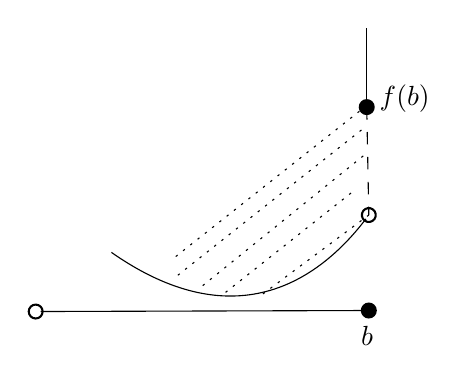
\begin{tikzpicture}[x=0.75pt,y=0.75pt,yscale=-1,xscale=1]
%uncomment if require: \path (0,300); %set diagram left start at 0, and has height of 300

%Straight Lines [id:da1885857134189366] 
\draw    (72.85,140.49) -- (231,140) ;
\draw [shift={(231,140)}, rotate = 359.82] [color={rgb, 255:red, 0; green, 0; blue, 0 }  ][fill={rgb, 255:red, 0; green, 0; blue, 0 }  ][line width=0.75]      (0, 0) circle [x radius= 3.35, y radius= 3.35]   ;
\draw [shift={(70.5,140.5)}, rotate = 359.82] [color={rgb, 255:red, 0; green, 0; blue, 0 }  ][line width=0.75]      (0, 0) circle [x radius= 3.35, y radius= 3.35]   ;
%Curve Lines [id:da2140869189476351] 
\draw    (107,112) .. controls (165.8,153.16) and (206.35,126.37) .. (229.6,95.87) ;
\draw [shift={(231,94)}, rotate = 306.35] [color={rgb, 255:red, 0; green, 0; blue, 0 }  ][line width=0.75]      (0, 0) circle [x radius= 3.35, y radius= 3.35]   ;
%Straight Lines [id:da7101268307932742] 
\draw  [dash pattern={on 0.84pt off 2.51pt}]  (180,132) -- (231,94) ;
%Straight Lines [id:da11465558063145465] 
\draw  [dash pattern={on 0.84pt off 2.51pt}]  (139,123) -- (230,51) ;
%Straight Lines [id:da14838712360943784] 
\draw  [dash pattern={on 0.84pt off 2.51pt}]  (151,128) -- (230.5,63.75) ;
%Straight Lines [id:da3698546574606112] 
\draw  [dash pattern={on 0.84pt off 2.51pt}]  (138,114) -- (229,42) ;
%Straight Lines [id:da9225721961115954] 
\draw    (230,42) -- (230,4) ;
%Straight Lines [id:da857277784452775] 
\draw  [dash pattern={on 4.5pt off 4.5pt}]  (230,42) -- (231,94) ;
\draw [shift={(230,42)}, rotate = 88.9] [color={rgb, 255:red, 0; green, 0; blue, 0 }  ][fill={rgb, 255:red, 0; green, 0; blue, 0 }  ][line width=0.75]      (0, 0) circle [x radius= 3.35, y radius= 3.35]   ;
%Straight Lines [id:da07189727817210678] 
\draw  [dash pattern={on 0.84pt off 2.51pt}]  (162,131.25) -- (224.5,81.75) ;

% Text Node
\draw (226,146.4) node [anchor=north west][inner sep=0.75pt]    {$b$};
% Text Node
\draw (235,29.9) node [anchor=north west][inner sep=0.75pt]    {$f( b)$};


\end{tikzpicture}

\caption{Visualization of convex function.}\label{fig:conx_supersemi}
\end{figure}
1. and 2. are therefore proved. To prove 3. for sequence $\{x_i\}\subseteq (a,b)$ with $x_i\to b$, we have sequence $\{\lambda_i\}$ s.t. $x_i=\lambda_i c +(1-\lambda_i)b$ (where $c\le \min x_i$). We have $\lambda_i\to 0$ since $x_i\to b$. From convex, we have $g(x_i)\le \lambda_i g(c)+(1-\lambda_i) g(b)$. Take $\limsup$ from both sides, we have
$$\limsup g(x_i)\le g(b).$$
The other endpoint can be proved similarly. We therefore have proved 3.

``$\Rightarrow$'':
For any interior interval $[c,d]$ for \tb{any} $a<c<d<b$ from 1. and 2., we get \cref{eq:fbcd} (actually  according to \cite[Theorem 5.4.3]{mtnotes}, 1. is implied by 2.), and \cref{eq:bgfda}. And convex over any $[c,d]$ is achieved by \cref{rem:alc}. In other words, convex over $(c,d)$ is achieved. To get convex over $(c,d]$ if $g(d)<\infty$, for sequence $\{x_i\}\subseteq (a,b)$ with $x_i\to b$, if $x=\lambda c +(1-\lambda)b$, we have sequence $\{\lambda_i\}$ s.t. $\lambda_i\to \lambda$ and $x=\lambda_i c+(1-\lambda_i)x_i$. We then have $f(x)\le \lambda_i f(c)+(1-\lambda_i)f(x_i)$. Take $\limsup$ from both sides, we have 
$$f(x)\le  \lambda f(c)+(1-\lambda)f(b)$$
We therefore have proved $g$ is convex over $\Delta$ with inclusion of one or both endpoints.
\begin{rema}
Note here \cref{lem:setm} cannot be used to prove the endpoint since we only have continuous over $(a,b)$.
\end{rema}
\end{proof}

\begin{cora}\bfs{convexity criterion for smooth functions on $\mathbf{R}^{n}$}\label{cora:2_diff}
Let $f: \mathbf{R}^{n} \rightarrow \mathbf{R} \cup\{+\infty\}$ be a function. Assume that the domain $M$ of $f$ is a convex set and that $f$ is
\begin{enumerate}
    \item continuous on $M$
    \item twice differentiable on  $\ri M$.
\end{enumerate}
Then $f$ is convex $\Longleftrightarrow$ if its Hessian is positive semidefinite on  $\ri M$ :
\begin{align*}
h^{\top} f^{\prime \prime}(x) h \geq 0 \quad \forall x \in \operatorname{ri} M, \forall h \in \mathbf{R}^{n}
\end{align*}
\end{cora}
\begin{proof}\color{ForestGreen}
``$\Rightarrow$'': if $f$ is convex and $x \in \operatorname{ri} M$, then the function of one variable
\begin{align}
g(t)=f(x+t h)\label{eq:ffbac}
\end{align}
( $h$ is an arbitrary fixed direction in $\mathbf{R}^{n}$ ) is convex in certain neighborhood of the point $t=0$ on the axis. Since $f$ is twice differentiable in a neighborhood of $x, g$ is twice differentiable in a neighborhood of $t=0$, so that $g^{\prime \prime}(0)=h^{\top} f^{\prime \prime}(x) h \geq 0$ by \cref{thm:ccusf}.

``$\Leftarrow$'': Let us first prove that $f$ is convex on the relative interior $M^{\prime}$ of the domain $M$. First, clearly, $\ri M$ is a convex set. From \cref{thm:conx2onev}, all we should prove is that every one-dimensional function
\begin{align*}
g(t)=f(x+t(y-x)), \quad 0 \leq t \leq 1
\end{align*}
$\left(x\right.$ and $y$ are from $\ri M$ ) is convex on the segment $0 \leq t \leq 1$. Since $f$ is continuous on $M \supset\ri M$, $g$ is continuous on the segment; and since $f$ is twice continuously differentiable on $\ri M$, $g$ is continuously differentiable on $(0,1)$ with the second derivative
\begin{align*}
g^{\prime \prime}(t)=(y-x)^{\top} f^{\prime \prime}(x+t(y-x))(y-x) \geq 0
\end{align*}
By using \cref{lem:setm} twice, one is $(0,1)$ to $[0,1]$, the other is $\ri M$ to $M$, we have $f$ is convex over entire $M$.
\end{proof} 

\subsection{Lipschitz Continuity of Convex Functions}
\subsubsection{Lipschitz Continuity}
Convex functions possess very nice \tb{local} properties. However, before showing this, we first show a \tb{global} Lipschitz continuity of general \tb{continuous (not necessarily convex)} functions with \tb{strong assumptions of differentiability of $f$ and boundedness of $f'$}:
\begin{thma}\bfs{\cite[Theorem 9.19]{rudin1976principles}}\label{thm:re_919}
Suppose \tb{continuous} function $f$ maps a \tb{convex} open set $E \subset \mathbf{R}^{n}$ into $\mathbf{R}^{m}$, $f$ is differentiable in $E$, and there is a real number $L$ such that $\left\|{f}^{\prime}({x})\right\|_2 \leq L$
Then
\begin{align*}
|f(x)-f(y)| \leq L\|x-y\|_2
\end{align*}
for all $x\in E, y\in E .$
\end{thma}
\begin{rema}
``open'' is for differentiable at every point and can be replaced by any convex set $E$ similar to \cref{lem:setm} using sequence. In other words, \cref{thm:re_919} can be restated as:  in $\ri E$, continuous function $f$ is differentiable, and there is a real number $L$ such that $\left\|{f}^{\prime}({x})\right\| \leq L$, we then have $|f(x)-f(y)| \leq L\|x-y\|$ for all $x,y\in E$.
\end{rema}
\begin{proof}\color{ForestGreen}
We still defined $g(t)$ as in \cref{eq:ffbac}. We then have
\begin{align*}
g^{\prime}(t)=f^{\prime}(x+t(y-x))(y-x) 
\end{align*}
so that 
\begin{align*}
g^{\prime}(t)\leq L\|x-y\|
\end{align*}
for all $t \in[0,1]$, where convexity ensures $x+t(y-x)\in E$. By \cite[Theorem 5.19]{rudin1976principles}, we have
\begin{align*}
|{g}(1)-{g}(0)| \leq L|b-a|
\end{align*}
But ${g}(0)={f}(x)$ and ${g}(1)={f}(y)$. This completes the proof.
\end{proof}
\begin{cora}
If in addition, ${f}^{\prime}({x})={0}$ for all ${x} \in E$, then ${f}$ is constant (set $L=0$).
\end{cora}
\begin{rema}\bfs{explanation}
Convex of $E$ is also necessary in this corollary, if only open, then $f$ can be different constant on different disjoint subsets, convex here is essential to ensure the points on the lines between any pair points is in the domain to make sure constant over the total domain.

Also please note here $f^{\prime}=0$ almost everywhere cannot guarantee constant, see cantor function. So that means continuous almost everywhere is not the same as continuous.
\end{rema}

We next show a \tb{local Lipschitz continuity} over a closed bounded set in relative interior of the domain without any assumption of the differential or boundedness of $f'$:
\begin{thma}\bfs{boundedness and Lipschitz continuity of convex function}\label{thm:lip_conv}
Let $f$ be a convex function and let $K$ be a  \tb{closed  and  bounded set contained in the $\ri \dom f$}. Then $f$ is Lipschitz continuous on $K$: there exists constant $L$ for $K$, such that
\begin{align*}
|f(x)-f(y)| \leq L\|x-y\|_2 \quad \forall x, y \in K
\end{align*}
In particular, $f$ is bounded on $K$.
\end{thma}
\begin{rema}
All three assumptions on $K$: \circled{1} closeness, \circled{2} boundedness and the assumption \circled{3} $K \subset \ri \dom f$, are essential, as it is seen from the following  examples:
\begin{itemize}
    \item $f(x)=1 / x$,  $\dom f=(0,+\infty), K=(0,1]$. We have \circled{2} \circled{3} and not  \circled{1}; $f$ is neither bounded, nor Lipschitz continuous on $K$.
    \item $f(x)=x^{2}$, $\dom f=\mathbf{R}, K=\mathbf{R}$. We have \circled{1} \circled{3} and not \circled{2}; $f$ is neither bounded nor Lipschitz continuous on $K$.
    \item $f(x)=-\sqrt{x}$, $\dom f=[0,+\infty), K=[0,1] .$ We have \circled{1} \circled{2} and not \circled{3}; $f$ is not Lipschitz continuous on $K$, although is bounded: $\lim _{t \rightarrow+0} \frac{f(0)-f(t)}{t}=\lim _{t \rightarrow+0} t^{-1 / 2}=+\infty$, while for a Lipschitz continuous $f$, the ratios $t^{-1}(f(0)-f(t))$ should be bounded.
\end{itemize}
\end{rema}
\begin{proof}\color{ForestGreen}
We will start with the following a local version of the theorem.

\begin{lema}\label{lem:llll}
Let $f$ be a convex function, and let $\bar{x} \in \ri \dom f$. Then
\begin{enumerate}[1).]
    \item $f$ is bounded around $\bar{x}$: there exists a positive $r$ such that $f$ is bounded in the $r$-neighborhood $U_{r}(\bar{x})$ of $\bar{x}$ in the $\Aff \dom f$ :
\begin{align*}
\exists r>0, C: \quad|f(x)| \leq C \quad \forall x \in U_{r}(\bar{x})=\{x \mid x \in \operatorname{Aff}(\dom f),\| x-\bar{x} \|_2 \leq r\}
\end{align*}
\item $f$ is Lipschitz continuous around $\bar{x}$: there exists a positive $\rho$ and a constant $L$ such that
\begin{align*}
\left|f(x)-f\left(x^{\prime}\right)\right| \leq L\|x-x^{\prime}\|_2, \forall x, x^{\prime} \in U_{\rho}(\bar{x})
\end{align*}
\end{enumerate}
\end{lema} 
\begin{proof}\color{ForestGreen} of {lem:llll}

Proof of 1).

Since $\bar{x}\in \ri \dom f$, there exists a neighborhood $U_{\bar{r}}(\bar{x})\subseteq\dom f$. Now, we can find a small simplex $\Delta$ of the dimension $m=\operatorname{dim}\Aff(\dom  f)$ with the vertices $x_{0}, \ldots, x_{m}$ in $U_{\bar{r}}(\bar{x})$ in such a way that $\bar{x}$ will be a convex combination of the vectors $x_{i}$ with positive coefficients, even with the coefficients $1 /(m+1)$ :
\begin{align*}
\bar{x}=\sum_{i=0}^{m} \frac{1}{m+1} x_{i}
\end{align*}
We know that $\bar{x}\in \ri \Delta$ from \cref{cora:pos_int}. Since $\Delta$ spans the same affine set as $\dom  f$, it means that $\Delta$ contains $U_{r}(\bar{x})$ with certain $r>0$. Now, from \cref{co:b_f_ex}, in
\begin{align*}
\Delta=\left\{\sum_{i=0}^{m} \lambda_{i} x_{i} \mid \lambda_{i} \geq 0, \sum_{i} \lambda_{i}=1\right\}
\end{align*}
$f$ is bounded from above by the quantity $\max _{0 \leq i \leq m} f\left(x_{i}\right)$ by Jensen's inequality:
\begin{align*}
f\left(\sum_{i=0}^{m} \lambda_{i} x_{i}\right) \leq \sum_{i=0}^{m} \lambda_{i} f\left(x_{i}\right) \leq \max _{i} f\left(x_{i}\right)
\end{align*}
Consequently, $f$ is \tb{bounded from above}, by the same quantity, in $U_{r}(\bar{x})$.


\begin{figure}[H]
\centering


\tikzset{every picture/.style={line width=0.75pt}} %set default line width to 0.75pt        

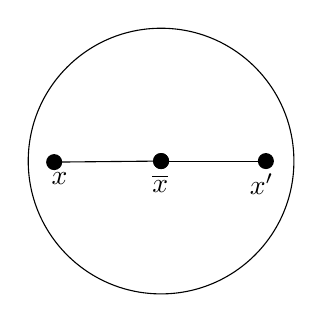
\begin{tikzpicture}[x=0.75pt,y=0.75pt,yscale=-1,xscale=1]
%uncomment if require: \path (0,300); %set diagram left start at 0, and has height of 300

%Straight Lines [id:da13368339552233044] 
\draw    (119,111.25) -- (170.5,110.75) ;
\draw [shift={(170.5,110.75)}, rotate = 359.44] [color={rgb, 255:red, 0; green, 0; blue, 0 }  ][fill={rgb, 255:red, 0; green, 0; blue, 0 }  ][line width=0.75]      (0, 0) circle [x radius= 3.35, y radius= 3.35]   ;
\draw [shift={(119,111.25)}, rotate = 359.44] [color={rgb, 255:red, 0; green, 0; blue, 0 }  ][fill={rgb, 255:red, 0; green, 0; blue, 0 }  ][line width=0.75]      (0, 0) circle [x radius= 3.35, y radius= 3.35]   ;
%Straight Lines [id:da21549014047251047] 
\draw    (170.5,110.75) -- (221,110.75) ;
\draw [shift={(221,110.75)}, rotate = 0] [color={rgb, 255:red, 0; green, 0; blue, 0 }  ][fill={rgb, 255:red, 0; green, 0; blue, 0 }  ][line width=0.75]      (0, 0) circle [x radius= 3.35, y radius= 3.35]   ;
\draw [shift={(170.5,110.75)}, rotate = 0] [color={rgb, 255:red, 0; green, 0; blue, 0 }  ][fill={rgb, 255:red, 0; green, 0; blue, 0 }  ][line width=0.75]      (0, 0) circle [x radius= 3.35, y radius= 3.35]   ;
%Shape: Circle [id:dp7937136617849974] 
\draw   (106.5,110.75) .. controls (106.5,75.4) and (135.15,46.75) .. (170.5,46.75) .. controls (205.85,46.75) and (234.5,75.4) .. (234.5,110.75) .. controls (234.5,146.1) and (205.85,174.75) .. (170.5,174.75) .. controls (135.15,174.75) and (106.5,146.1) .. (106.5,110.75) -- cycle ;

% Text Node
\draw (116.5,115.23) node [anchor=north west][inner sep=0.75pt]    {$x$};
% Text Node
\draw (165,116.23) node [anchor=north west][inner sep=0.75pt]    {$\overline{x}$};
% Text Node
\draw (212,115.73) node [anchor=north west][inner sep=0.75pt]    {$x'$};


\end{tikzpicture}

\caption{Visualization of proof.}\label{fig:proof_f22}
\end{figure}
 Now let us prove that if $f$ is above bounded, by some $W$, in $U_{r}(\bar{x})$, then it in fact is \tb{below bounded} in this neighborhood (and, consequently, is bounded in $U_{r}$ ). 
 
 Indeed, let $x \in U_{r}(\bar{x})$ s.t. $|x-\bar{x}| \leq r$. Setting $x^{\prime}=\bar{x}-[x-\bar{x}]=2 \bar{x}-x$, we get  $\left|x^{\prime}-\bar{x}\right|=|x-\bar{x}| \leq r$ and $x^{\prime} \in\Aff(\dom f)$, so that $x^{\prime} \in U_{r}(\bar{x})$. Since $\bar{x}=\frac{1}{2}\left[x+x^{\prime}\right]$ we have
\begin{align*}
2 f(\bar{x}) \leq f(x)+f\left(x^{\prime}\right)
\end{align*}
whence
\begin{align*}
f(x) \geq 2 f(\bar{x})-f\left(x^{\prime}\right) \geq 2 f(\bar{x})-W, \quad x \in U_{r}(\bar{x})
\end{align*}
and $f$ indeed is below bounded in $U_{r}(\bar{x})$.


Proof of 2).

 2). is an immediate consequence of 1). Indeed, let us prove that $f$ is Lipschitz continuous in the neighborhood $U_{r / 2}(\bar{x})$, where $r>0$ is such that $f$ is bounded in $U_{r}(\bar{x})$ from 1). Let $|f| \leq C$ in  $U_{r}(\bar{x})$, and let $x, x^{\prime} \in U_{r / 2}(\bar{x}), x \neq x^{\prime} .$ Let us extend the segment $\left[x, x^{\prime}\right]$ through the point $x^{\prime}$ until it reaches, at certain point $x^{\prime \prime}$, the (relative) boundary of $U_{r}$; then we will get
 \begin{align*}
x^{\prime} \in\left(x, x^{\prime \prime}\right) ; \quad\left|x^{\prime \prime}-\bar{x}\right|=r
\end{align*}
 \begin{figure}[H]
\centering


\tikzset{every picture/.style={line width=0.75pt}} %set default line width to 0.75pt        

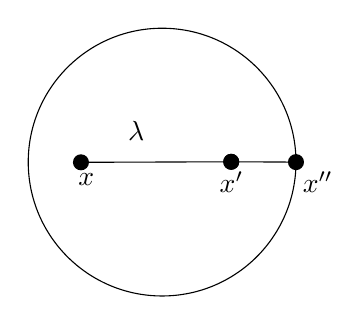
\begin{tikzpicture}[x=0.75pt,y=0.75pt,yscale=-1,xscale=1]
%uncomment if require: \path (0,300); %set diagram left start at 0, and has height of 300

%Straight Lines [id:da13368339552233044] 
\draw    (119,111.25) -- (191.4,111) ;
\draw [shift={(191.4,111)}, rotate = 359.8] [color={rgb, 255:red, 0; green, 0; blue, 0 }  ][fill={rgb, 255:red, 0; green, 0; blue, 0 }  ][line width=0.75]      (0, 0) circle [x radius= 3.35, y radius= 3.35]   ;
\draw [shift={(119,111.25)}, rotate = 359.8] [color={rgb, 255:red, 0; green, 0; blue, 0 }  ][fill={rgb, 255:red, 0; green, 0; blue, 0 }  ][line width=0.75]      (0, 0) circle [x radius= 3.35, y radius= 3.35]   ;
%Straight Lines [id:da21549014047251047] 
\draw    (191.4,111) -- (222.6,111.15) ;
\draw [shift={(222.6,111.15)}, rotate = 0.28] [color={rgb, 255:red, 0; green, 0; blue, 0 }  ][fill={rgb, 255:red, 0; green, 0; blue, 0 }  ][line width=0.75]      (0, 0) circle [x radius= 3.35, y radius= 3.35]   ;
\draw [shift={(191.4,111)}, rotate = 0.28] [color={rgb, 255:red, 0; green, 0; blue, 0 }  ][fill={rgb, 255:red, 0; green, 0; blue, 0 }  ][line width=0.75]      (0, 0) circle [x radius= 3.35, y radius= 3.35]   ;
%Shape: Circle [id:dp5723541462981179] 
\draw   (93.6,111.15) .. controls (93.6,75.53) and (122.48,46.65) .. (158.1,46.65) .. controls (193.72,46.65) and (222.6,75.53) .. (222.6,111.15) .. controls (222.6,146.77) and (193.72,175.65) .. (158.1,175.65) .. controls (122.48,175.65) and (93.6,146.77) .. (93.6,111.15) -- cycle ;

% Text Node
\draw (116.5,115.23) node [anchor=north west][inner sep=0.75pt]    {$x$};
% Text Node
\draw (184.6,114.63) node [anchor=north west][inner sep=0.75pt]    {$x'$};
% Text Node
\draw (224.6,114.55) node [anchor=north west][inner sep=0.75pt]    {$x''$};
% Text Node
\draw (140.5,90.23) node [anchor=north west][inner sep=0.75pt]    {$\lambda $};


\end{tikzpicture}

\end{figure}

By the convexity of $f$ we have for $\lambda=\frac{\|x^{\prime}-x\|_2}{\|x^{\prime \prime}-x\|_2} \in(0,1)$,
\begin{align*}
f\left(x^{\prime}\right)-f(x) \leq \lambda\left(f\left(x^{\prime \prime}\right)-f(x)\right) =\|x^{\prime}-x\|_2 \frac{f\left(x^{\prime \prime}\right)-f(x)}{\|x^{\prime \prime}-x\|_2}
\end{align*}
The second factor in the right hand side does not exceed the quantity $(2 C) /(r / 2)=$ $4 C / r$. Thus, we have
\begin{align*}
f\left(x^{\prime}\right)-f(x) \leq(4 C / r)\|x^{\prime}-x\|_2, \forall x, x^{\prime} \in U_{r / 2}
\end{align*}
swapping $x$ and $x^{\prime}$, we come to
\begin{align*}
f(x)-f\left(x^{\prime}\right) \leq(4 C / r)\|x^{\prime}-x\|_2
\end{align*}
whence
\begin{align*}
|f(x)-f\left(x^{\prime}\right)| \leq(4 C / r)\|x-x^{\prime}\|_2, x, x^{\prime} \in U_{r / 2}
\end{align*}
as required in 2).
\end{proof}


After \cref{lem:llll}, we next prove \cref{thm:lip_conv}: 
Assume, on contrary, that $f$ is not Lipschitz continuous on $K ;$ then for every integer $i$ there exists a pair of points $x_{i}, y_{i} \in K$ such that
\begin{align}
f\left(x_{i}\right)-f\left(y_{i}\right) \geq i\|x_{i}-y_{i}\|_2\label{eq:fbanf}
\end{align}
Since $K$ is \tb{compact}, passing to a subsequence we can ensure that $x_{i} \rightarrow x \in K$ and $y_{i} \rightarrow y \in K$. 

By \cref{lem:llll}, the case $x=y$ is impossible since we have shown $f$ is Lipschitz continuous in a neighborhood of $x=y$ and the ratios $\left(f\left(x_{i}\right)-f\left(y_{i}\right)\right) /\|x_{i}-y_{i}\|_2$ form a bounded sequence, which we know is not the case. Thus, the case $x=y$ is impossible. 

The case $x \neq y$ is also impossible. From \cref{lem:llll}, we know $f$ is continuous on  $\ri \dom f$ at both the points $x$ and $y$ so that we would have $f\left(x_{i}\right) \rightarrow f(x)$ and $f\left(y_{i}\right) \rightarrow f(y)$ as $i \rightarrow \infty$. Thus, the left hand side in \cref{eq:fbanf} remains bounded as $i \rightarrow \infty$ while the right hand side tends to $\infty$ as $i \rightarrow \infty$; this is the desired contradiction.
\end{proof} 

\subsubsection{Directional Derivative and  Bounded Below}
In what follows in this section, for the sake of conciseness, WLOG, we will assume that the the domain of $f$ is full dimensional, meaning that  $\Aff(\dom f)=\mathbf{R}^{n}$. We can get the general case by translating the corresponding statements for the case when $\Aff(\dom f)$ is smaller than the whole $\mathbf{R}^{n}$: interior becomes relative interior, $h \in \mathbf{R}^{n}$ becomes $h \in V$, such that $\Aff(\dom f)=x_0+V$, etc.
\paragraph{Directional Derivative}
\begin{defa}\bfs{Directional Derivative}\label{def:dir_deri}
 Let $x \in \dom f$. We call the function $f$ \tb{differentiable in the direction} $h$ at $x$ if the following limit \tb{exists}:
\begin{align*}
f_{h}^{\prime}(x)=\lim _{t \downarrow 0} \frac{f(x+h t)-f(x)}{t}
\end{align*}
\end{defa}
\begin{rema}\label{rem:vcxaa}
If $f'$ exists, $f_{h}^{\prime}(x)=f'h=\nabla f^{\top} h$, see \cite[Page 217 (39)]{rudin1976principles}. Please note here we need the \tb{right-hand limit}  $\lim _{t \downarrow 0}$, not $\lim _{t \to 0}$.
\end{rema}
\begin{thma}\bfs{directional differentiability of convex functions}$\quad$

Convex function $f$ is differentiable in \tb{any direction} $h \in \mathbf{R}^{n}$ at \tb{any point} $x \in\inte \dom  f$.
\end{thma}
\begin{rema}\bfs{explanation}\label{re:cas}
It means for any $x\in \ri \dom f$, the domain of function $s_x(h)\coloneqq f'_h(x)$ is $\mathbf{R}^n$.
\end{rema}
\begin{proof}\color{ForestGreen}
Let $x \in\inte \dom f$. Consider the function of one variable
\begin{align}
g(t)\coloneqq f(x+t h). \label{eq:ffbaccac}
\end{align}
and the function
\begin{align}
\phi(t)\coloneqq \frac{g(t)-g(0)}{t}, t>0 \label{eq:ffbac1}
\end{align}
For small enough $t$, we have $x+t h$ is inside $\dom f$ since $x\in \inte \dom f$. We then have $g(t)$ is \tb{convex} on a small neighbour $[-r,r]$. $g(t)$ is a univariate function, so from \cref{eq:real_conx2}, we know $\phi(t)$ is \tb{increasing} for $t\in (0,r)$. From \cref{thm:lip_conv}, we know $g(t)$ is Lipschitz continuous on $[-r,r]$ which implies $\phi(t)$ is bounded for $t\in (0,r]$. We then have the existence of right-hand limit $\phi(0+)$ from  \cite[Theorem 4.29]{rudin1976principles}, which equals $g'(0+)=f_{h}^{\prime}(x)$.
\end{proof}

\paragraph{Below Boundedness}
\cref{thm:lip_conv} says that a convex function $f$ is \tb{bounded on every compact subset  of $\ri \dom f$}. In fact there is much stronger statement on the \tb{below boundedness} of $f$: $f$ is below bounded on \tb{any bounded subset} of $\mathbf{R}^{n}$. This results is an immediate consequence of the following lower bound:

\begin{lema}{\bfs{global lower bound}}\label{lemacca}
 Let $f$ be a convex function and $x \in\inte \dom f$. Then $f_{h}^{\prime}(x)$ is \tb{convex positive homogenous (of degree 1) function} of $h$, and for any $y \in \dom f$
\begin{align}
f(y) \geq f(x)+f_{y-x}^{\prime}(x)\label{eq:mbnd}
\end{align}
\end{lema}
\begin{rema}
With $h=y-x$, in terms of $g(t)$ defined in \cref{eq:ffbaccac}, it says $g(1)\geq g(0)+g'(0+)$. Intuitively, this is true, from the increasing of $\phi(t)$.
\end{rema}
\begin{proof}\color{ForestGreen}
Let us prove first that the directional derivative is homogenous. Indeed, for any $h \in \mathbf{R}^{n}$ and $\tau>0$
\begin{align*}
f_{\tau h}^{\prime}(x)=\lim _{t \downarrow 0} \frac{f(x+\tau h t)-f(x)}{t}=\tau \lim _{\alpha \downarrow 0} \frac{f(x+h \alpha)-f(x)}{\alpha}=\tau f_{h}^{\prime}(x)
\end{align*}
Further, for any $h_{1}, h_{2} \in \mathbf{R}^{n}$, and $\lambda \in[0,1]$, by the convexity of $f$ we get
\begin{align*}
\begin{aligned}
f_{\lambda h_{1}+(1-\lambda) h_{2}}^{\prime}(x) &=\lim _{t \downarrow 0} \frac{1}{t}\left[f\left(x+\left(\lambda h_{1}+(1-\lambda) h_{2}\right) t\right)-f(x)\right] \\
& \leq \lim _{t \downarrow 0} \frac{1}{t}\left\{\lambda\left[f\left(x+t h_{1}\right)-f(x)\right]+(1-\lambda)\left[f\left(x+t h_{2}\right)-f(x)\right]\right\} \\
&=\lambda f_{h_{1}}^{\prime}(x)+(1-\lambda) f_{h_{2}}^{\prime}(x)
\end{aligned}
\end{align*}

Thus $f_{h}^{\prime}(x)$ is convex in $h$. Finally, let $t \in(0,1], y \in \dom f$ and
\begin{align*}
y_{t}=x+t(y-x)=(1-t) x+t y
\end{align*}
Then
\begin{align*}
f(y)=f\left(y_{t}+\frac{1}{t}(1-t)\left(y_{t}-x\right)\right) \geq f\left(y_{t}\right)+\frac{1-t}{t}\left[f\left(y_{t}\right)-f(x)\right]
\end{align*}
(the latter inequality is nothing but the convexity property of $\left.f: f\left(y_{t}\right) \leq t f(y)+(1-t) f(x)\right)$ and we conclude \cref{eq:mbnd} taking the limit as $t \downarrow 0$.
\end{proof}
\begin{cora}\bfs{a restatement}\label{cora:sx_conv}
$s_x(h)\coloneqq f'_h(x)$ is convex in $h$ and positive homogenous (of degree 1), with $\dom s_x(h)=\mathbf{R}^n$.
\end{cora}
\begin{cora}\bfs{below boundedness}\label{cora:beboud}

\centerline{$f$ is below bounded on \tb{any bounded subset} of $\mathbf{R}^{n}$}
\end{cora}
\begin{rema}
We will give a another simple proof in \cref{cora:cora:beboud1}, which will not use the directional derivative.
\end{rema}
\begin{proof}\color{ForestGreen}
As in \cref{re:cas},  $s_x(h)$ has domain $\mathbf{R}^n$. For any \tb{bounded subset} $K\subseteq \dom f$,  $s_x(y-x)$ is then bounded since  $s_x(h)$ is convex and $K-x$ is bounded closed (and in interior of $\mathbf{R}^n$ of course) as required by \cref{thm:lip_conv}. Below bounded is then from \cref{eq:mbnd}.
\end{proof}
\begin{cora}
Convex function $f$ can achieve the infimum on a \tb{bounded closed} set $B$ which intersects $\dom f$ (not necessarily $\subseteq \dom f$ ).
\end{cora}
\begin{rema}
For examples, relative entropy $D(\cdot||Q)$ can achieve the infimum on any closed subset of $\Delta\cap \dom D(\cdot||Q)$, where $\Delta$ is the probability simplex.
\end{rema}
\begin{proof}\color{ForestGreen}
Since $f$ is  below bounded on $B$, $\inf_B f$ exist. For $\epsilon>0$, $C\coloneqq \{x\mid f(x) \le \inf_B f+\epsilon \}$ is the sublevel set of $f$ and is convex and closed (because of continuous \cref{thm:eq_cl_cl}). For $B\cap C\subseteq \dom f $ which is compact, $f$ is continuous, we have that $f$ can achieve $\inf_B f$.
\end{proof}


\subsection{Subgradients of Convex Functions}
\subsubsection{Definitions and Theorems}
We are now ready to introduce a "good surrogate" of the notion of the gradient for a convex function. 
\begin{defa}\bfs{Subgradient of Convex Function}
 Let $f$ be function (not necessarily convex). A vector $h$ is called \tb{subgradient} of function $f$ at a point $x \in \dom f$ if for \tb{any} $y \in \dom f$ we have
\begin{align}
f(y) \geq f(x)+h^{\top}(y-x)\label{eq:sub_h}
\end{align}
The set $\partial f(x)$ of all subgradients of $f$ at $x$ is called the \tb{subdifferential} of $f$ at the point $x$. 
\end{defa}
\begin{rema}\bfs{explanation}
This definition says: for a subgradient $h$, it means there exists an \tb{affine minorant} $h^{\top} x-a$ of $f$ which \tb{coincides} with $f$ at $x$ :
\begin{align*}
f(y) \geq h^{\top} y-a , \forall y, \text{ and } f(x)=h^{\top} x-a
\end{align*}
In the following, we will also see \cref{eq:mbnd} $f(y) \geq f(x)+f_{y-x}^{\prime}(x)$ is just an inequality with a special $h$ in \cref{eq:sub_h} with $h$ being selected in \cref{eq:sub_fff}.
\end{rema}
\begin{figure}
    \centering
    \includegraphics[width=0.5\textwidth]{Figs/6.png}
    \caption{if \tb{differentiable}, $(\nabla f(x),-1)$ defines a supporting hyperplane to the epigraph.}
    \label{fig:supp_conx1}
\end{figure}
\begin{rema}
Affine function $\alpha y=h^{\top} x-a$ must have $\alpha\ne 0$, $y\in \mathbf{R}$ and $x,h\in\mathbf{R}^n$. It is a \tb{non-vertical} hyperplane in $\mathbf{R}^{n+1}$, i.e. cannot be be a hyperplane $0=h^{\top} x-a$.
\end{rema}
The most elementary properties of the subgradients are summarized in the following theorem:
\begin{thma}\bfs{subgradient of convex functions}\label{thm:sub_convxf}
Let $f$ be a convex function and $x$ be a point from $\inte \dom f$. Then
\begin{enumerate}[1).]
    \item $\partial f(x)$ is a \tb{closed convex set} which for sure is \tb{nonempty and bounded}.
    \item for any $d \in \mathbf{R}^{n}$
\begin{align}
f_{m}^{\prime}(x)=\max \left\{h^{\top} m \mid h\in \partial f(x)\right\}\label{eq:sub_fff}
\end{align}
In other words, the directional derivative is nothing but the \tb{support function} of the set $\partial f$.
\item If $f$ is differentiable at $x$, then $\partial f(x)=\{\nabla f(x)\}$, a singleton.
\end{enumerate} 
\end{thma}
\begin{rema}
$\partial f$ at $x$ \tb{may be empty if $x$ is a boundary point of the domain}. See \cref{exm:nvd}.
\end{rema}
\begin{proof}\color{ForestGreen}
Proof of 1).

\tb{Closeness and convexity} of $\partial f(x)$ are evident: \cref{eq:sub_h} is an infinite system of nonstrict linear inequalities with respect to $h$, the inequalities being indexed by $y \in \mathbf{R}^{n}$. 

\tb{Nonemptiness} of $\partial f(x)$ for the case when $x \in \operatorname{int} \dom f$: Point $(f(x), x)$ belongs to the boundary of  $\Epi (f)$. Hence, from separation theorem there is a linear form $(-\alpha, h)$ which properly separates $x$ and  $\Epi (f)$
\begin{align}
h^{\top} y-\alpha \tau \leq h^{\top} x-\alpha f(x)\label{eq:fha}
\end{align}
for any $(\tau, y) \in \Epi(f)$, i.e. $\tau\ge f(y)$. Note that we can take
\begin{align}
\|h\|_2^{2}+\alpha^{2}=1\label{eq:norm_}
\end{align}
and such that $(-\alpha, h) \in\Aff \Epi (f))$. And since for any $\tau \geq f(x)$ the point $(\tau, x)$ belongs to the $\Epi(f)$, we conclude that $\alpha \geq 0$.

Now recall that a convex function is locally Lipschitz continuous on the interior of its domain. This means that there exist some $\epsilon>0$ and $M>0$ such that the ball of the radius $\epsilon$, centered at $x$, belongs to  $\inte \dom f$ (since $x\in \operatorname{int} \dom f$) and for any $y$ in this ball
\begin{align*}
f(y)-f(x) \leq L\|y-x\|_2
\end{align*}
Thus, for any $y$ in the ball
\begin{align*}
h^{\top}(y-x) \leq \alpha(f(y)-f(x)) \leq \alpha L\|y-x\|_2
\end{align*}
When choosing $y=x+\epsilon h$ we get $\|h\|_2^{2} \leq L \alpha\|h\|_2$ and together with the normalizing equation \cref{eq:norm_}, we have
\begin{align*}
\alpha \geq \frac{1}{\sqrt{1+L^{2}}}
\end{align*}
\tb{The vertical hyper-plane is therefore not possible.} Now from \cref{eq:fha}, with $\tau$ being $f(y)$, we can choose $\bar{h}=h / \alpha$ to get
\begin{align*}
f(y) \geq f(x)+\bar{h}^{\top}(y-x)
\end{align*}
\tb{Boundedness}: if $h \in \partial f(x), h \neq 0$, then by choosing $y=x+\epsilon h /\|h\|_2$, we obtain:
\begin{align*}
\epsilon\|h\|_2=h^{\top}(y-x) \leq f(y)-f(x) \leq L\|y-x\|_2=L \epsilon
\end{align*}
what implies the \tb{boundedness of $\partial f(x)$: $\|h\|_2\le L$.}


Proof of 2).

Note that, as $f_{0}^{\prime}(x)=0$, we have 
\begin{align}
f_{m}^{\prime}(x)-f_{0}^{\prime}(x)=f_{m}^{\prime}(x)=\lim _{t \downarrow 0} \frac{f(x+m t)-f(x)}{t} \geq h^{\top} m\label{eq:nbvc}
\end{align}
for any vector $h$ from $\partial f(x)$. Therefore, the subdifferential of the function $s_x(m)\coloneqq f_{m}^{\prime}(x)$ at $m=0$ exists and
\begin{align*}
\partial f(x) \subset \partial s_x(0)
\end{align*}
As $s_x(m)$ is convex in $m$ (cf. \cref{cora:sx_conv}), from definition of subgradient, we know
\begin{align*}
s_x(y-x)=s_x(y-x)-s_x(0) \geq h^{\top}(y-x)
\end{align*}
for any $h \in \partial s_x(0)$, and by \cref{lemacca} we have for any $y \in \dom  f$
\begin{align*}
f(y) \geq f(x)+f_{y-x}^{\prime}(x) \geq f(x)+h^{\top}(y-x) \text { for } h\in \partial  s_x(0)
\end{align*}
We conclude that $\partial  s_x(0) \subset \partial f(x)$. Therefore we have  $$\partial_{m} f_{0}^{\prime}(x)=\partial  s_x(0)   \equiv \partial f(x).$$
Let now $d_{m} \in \partial s_x(m)$ (which is not empty by 1). since $s_x(m)$ is convex and has domain $\mathbf{R}^n$). \tb{We prove this is the $h$ that achieves the maximum for the support function.}

We need first to prove $d_{m} \in \partial s_x(0)$, i.e. $d_{m} \in \partial f(x)$. For any $v \in \mathbf{R}^{n}$ and $\tau>0$ we have
\begin{align*}
\tau f_{v}^{\prime}(x)=f_{\tau v}^{\prime}(x) \geq f_{m}^{\prime}(x)+d_{m}^{\top}(\tau v-m)
\end{align*}
so that when $\tau \rightarrow \infty$ we obtain $f_{v}^{\prime}(x) \geq d_{m}^{\top} v$ what means that $d_{m} \in \partial s_x(0)$.

Next, when $\tau \rightarrow 0$ we get $f_{m}^{\prime}(x)-d_{m}^{\top} m \leq 0$ and by \cref{eq:nbvc} we conclude that $d_{m}^{\top} m=f_{m}^{\prime}(x)$, what implies 2). and $d_h$ is the one that achieves the maximum for the support function. 

Proof of 3).

If $x \in\inte \dom f$ and $f$ is differentiable at $x$, then $\nabla f(x) \in \partial f(x)$ by \cref{rem:vcxaa} and \cref{lemacca}. To prove that $\nabla f(x)$ is the \tb{only subgradient} of $f$ at $x$, note that if $h \in \partial f(x)$, then, by definition,
\begin{align*}
f(y)-f(x) \geq h^{\top}(y-x) \quad \forall y
\end{align*}
Substituting $y-x=t d, d$ being a fixed direction and $t$ being $>0$, dividing both sides of the resulting inequality by $t$ and passing to limit as $t \rightarrow+0$, we get
\begin{align*}
d^{\top} \nabla f(x) \geq h^{\top} d
\end{align*}
This inequality should be valid for all $d \in \mathbf{R}^{n}$, which is possible if and only if $h=\nabla f(x)$.
\end{proof}
\begin{exma}
\begin{align*}
f(x)=|x|
\end{align*}
on the axis. We have
\begin{align*}
\partial|x|= \begin{cases}\{-1\}, & x<0 \\ {[-1,1],} & x=0 \\ \{+1\}, & x>0\end{cases}
\end{align*}
\end{exma}
\begin{exma}\label{exm:nvd}
Note also that if $x$ is a boundary point of the domain of a convex function, $\partial f$ at $x$ may be empty, as it is the case with the function
\begin{align*}
f(y)= \begin{cases}-\sqrt{y}, & y \geq 0 \\ +\infty, & y<0\end{cases}
\end{align*}
it is clear that there is no non-vertical supporting line to the epigraph of the function at the point $(0, f(0))$, and, consequently, there is no affine minorant of the function which is exact at $x=0$
\end{exma}

\begin{cora}\bfs{converse of \cref{thm:sub_convxf}}\label{cora:conv_subvxf}
Let a continuous function $f$ be such that for \tb{any} $x \in\inte \dom f$ the subdifferential $\partial f(x)$ is \tb{not empty}. Then $f$ is convex.
\end{cora} 
\begin{proof}\color{ForestGreen}
Let $x, y \in\inte \dom f, 0 \leq \lambda \leq 1$ and $z=x+\lambda(y-x)(\in\inte \dom f)$. Let $h \in \partial f(z)$, then
\begin{align*}
\begin{aligned}
&f(y) \geq f(z)+h^{\top}(y-z)=f(z)+(1-\lambda) h^{\top}(y-x) \\
&f(x) \geq f(z)+h^{\top}(x-z)=f(z)-\lambda h^{\top}(y-x)
\end{aligned}
\end{align*}
and we can get 
\begin{align*}
\lambda f(y)+(1-\lambda) f(x) \geq f(z)
\end{align*}
the proof is completed using \cref{lem:setm}.
\end{proof}


\subsubsection{Subgradient Calculus}\label{sec:sub_cal}
As we already know from \cref{thm:sub_convxf}, the directional derivative $f_{h}^{\prime}(x)$ is the support function of the subdifferential $\partial f(x)$. \tb{This basic observation is the basis of our future developments.} We show the rule of computing subgradients of "composite" functions, like sums, superpositions, maxima, etc..

\paragraph{Weighted Sums}
If $f, g$ are convex functions on $\mathbf{R}^{n}$ and $\lambda, \mu>0$ then the subgradient of the function $h(x)=\lambda f(x)+\mu g(x)$ satisfies
\begin{align}
\partial h(x)=\lambda \partial f(x)+\mu \partial g(x)\label{eq:bmnac}
\end{align}
for any $x \in\inte \dom h$:
\begin{proof}\color{ForestGreen}
Let $x \in\inte \dom f \cap\inte \dom g$. Then for any $h \in \mathbf{R}^{n}$ we have by \cref{thm:sub_convxf}:
\begin{align*}
\begin{aligned}
f_{h}^{\prime}(x) &=\lambda f_{h}^{\prime}(x)+\mu g_{h}^{\prime}(x) \\
&=\max \left\{\lambda h^{\top} d_{1} \mid d_{1} \in \partial f(x)\right\}+\max \left\{\mu h^{\top} d_{2} \mid d_{2} \in \partial g(x)\right\} \\
&=\max \left\{h^{\top}\left(\lambda d_{1}+\mu d_{2}\right) \mid d_{1} \in \partial f(x), d_{2} \in \partial g(x)\right\} \\
&=\max \left\{h^{\top} d \mid d \in \lambda \partial f(x)+\mu \partial g(x)\right\}
\end{aligned}
\end{align*}
Using \cref{cora:sfcs}, together with $s_x(h)\coloneqq f_{h}^{\prime}(x)$ has domain $\mathbf{R}^n$, we obtain \cref{eq:bmnac}.
\end{proof}

\paragraph{Affine Substitution}
Let the function $f(y)$ be convex with  $\dom f \subset \mathbf{R}^{m}$. Consider the affine operator
\begin{align*}
\mathcal{A}: \mathbf{R}^{n} &\rightarrow \mathbf{R}^{m}\\
  x &\mapsto A x+b
\end{align*}
and $\phi(x)=f(\mathcal{A}(x))$.
Then for any $x \in \dom  \phi=\left\{x \in \mathbf{R}^{n} \mid \mathcal{A}(x) \in \dom  f\right\}$
\begin{align}
\partial \phi(x)=A^{\top}\partial f(\mathcal{A}(x))\label{eq:aff_subg}
\end{align}
\begin{proof}\color{ForestGreen}
 if $y=\mathcal{A}(x)$ then for any $h \in \mathbf{R}^{n}$ we have
\begin{align*}
\phi_{h}^{\prime}(x)=f_{A h}^{\prime}(y)=\max \left\{d^{\top}A h \mid d \in \partial f(y)\right\}=\max \left\{{d}^{\top}h \mid {d} \in A^{\top}\partial f(y)\right\}
\end{align*}
Now by \cref{thm:sub_convxf,cora:sfcs}, we get $\partial \phi(x)=A^{\top}\partial f(\mathcal{A}(x))$.
\end{proof}
\paragraph{Pointwise Sup} 
\tb{$\bullet$ Finite Supreme:}

We first state a special case with supreme taking over \tb{finite functions.}

Let $f=\sup _{i} f_{i}$ of a \tb{finite} family of convex functions on $\mathbf{R}^{n}$. Then its subgradient at any $x \in \inte \dom  f$ satisfies
\begin{align*}
\partial f=\operatorname{Conv}\left\{\partial f_{i} \mid i \in I(x)\right\}
\end{align*}
where $I(x)=\left\{i\mid  f_{i}(x)=f(x)\right\}$ is the set of functions $f_{i}$ which are \tb{active} at $x$.
\begin{proof}\color{ForestGreen}
Unfortunately, the above rule does not have a "closed form". However, it allows to compute elements of the subgradient.
\end{proof}
\begin{proof}\color{ForestGreen}
 let $x \in \cap_{i}\inte \dom f_{i}$, and assume that $I(x)=1, . ., k$. Then for any $h \in \mathbf{R}^{n}$ we have by \cref{thm:sub_convxf} and the definition of directional derivative:
\begin{align*}
f_{h}^{\prime}(x)=\lim _{t \downarrow 0} \frac{\max f_i(x+h t)-f(x)}{t} = \max _{1 \leq i \leq k} f_{i, h}^{\prime}(x)=\max _{1 \leq i \leq k} \max \left\{h^{\top}d_{i} \mid d_{i} \in \partial f_{i}(x)\right\}
\end{align*}
Note that for any numbers $a_{1}, \ldots, a_{k},$ we have
\begin{align*}
\max a_{i}=\max \left\{\sum_{i} \lambda_{i} a_{i} \mid \lambda \in \Delta_{k}\right\}
\end{align*}
where $\Delta_{k}=\left\{\lambda \geq 0, \sum_{i} \lambda_{i}=1\right\}$ is the standard simplex in $\mathbf{R}^{k}$. Thus
\begin{align*}
\begin{aligned}
f_{h}^{\prime}(x) &=\max _{\lambda \in \Delta_{k}} \sum_{i=1}^{k} \lambda_{i} \max \left\{h^{\top}d_{i} \mid d_{i} \in \partial f_{i}(x)\right\} \\
&=\max \left\{h^{\top}\left(\sum_{i=1}^{k} \lambda_{i} d_{i}\right) \mid d_{i} \in \partial f_{i}(x), \lambda \in \Delta_{k}\right\} \\
&=\max \left\{h^{\top}d \mid d=\sum_{i=1}^{k} \lambda_{i} d_{i}, d_{i} \in \partial f_{i}(x), \lambda \in \Delta_{k}\right\} \\
&=\max \left\{h^{\top}d \mid d \in \operatorname{Conv}\left\{\partial f_{i}(x), 1 \leq i \leq k\right\} .\right]
\end{aligned}
\end{align*}
\end{proof}

\tb{$\bullet$ General Supreme:}

We state the general case without proof:
\begin{lema}\label{lem:sup_convx_subg}
 Let $f=\sup _{\alpha \in \mathcal{F}} f_{\alpha}$ of an \tb{arbitrary} family $\mathcal{F}$ of convex and closed functions. Then for any $x$ from $\dom  f=\cap_{\alpha} \dom f_{\alpha}$, we have
\begin{align*}
\partial f(x) \supset \operatorname{Conv}\left\{\partial f_{\alpha}(x) \mid \alpha \in \alpha(x)\right\}
\end{align*}
where $\alpha(x)=\left\{\alpha \mid f_{\alpha}(x)=f(x)\right\}$. Furthermore, if the set $\mathcal{F}$ is \tb{compact (in some metric) and the function $\alpha \rightarrow f_{\alpha}(x)$ is closed,} then
\begin{align*}
\partial f(x)=\operatorname{Conv}\left\{\partial f_{\alpha}(x) \mid \alpha \in \alpha(x)\right\}
\end{align*}
\end{lema}
\paragraph{Examples}
\begin{exma}
Consider the function
\begin{align*}
f(x)=\sum_{i=1}^{m}\left|a_{i}^{\top}x-b_{i}\right|
\end{align*}
Let for $x \in \mathbf{R}^{n}$,
\begin{align*}
\begin{aligned}
I_{-}(x) &=\left\{i: a_{i}^{\top}x-b_{i}<0\right\} \\
I_{+}(x) &=\left\{i: a_{i}^{\top}x-b_{i}>0\right\} \\
I_{0}(x) &=\left\{i: a_{i}^{\top}x-b_{i}=0\right\}
\end{aligned}
\end{align*}
Then
\begin{align*}
\partial f(x)=-\sum_{i \in I_{-}(x)} a_{i}+\sum_{i \in I_{+}(x)} a_{i}+\sum_{i \in I_{0}(x)}\left[-a_{i}, a_{i}\right]
\end{align*}
Note here for set $I_{0}$, each $[-a_{i}, a_{i}]$ could also be viewed as $\Conv \{-a_{i}, a_{i}\}$ because $|x|$ is equivalent to $\max(x,-x)$.
\end{exma}
\begin{exma}
Consider the function $$f(x)=\max _{1 \leq i \leq n} x^{(i)},$$ where $x^{(i)}$ are the components of $x$ and denote $I(x)=\left\{i: x^{(i)}=f(x)\right\} .$ Then $$\partial f(x)=\operatorname{Conv}\left\{e_{i} \mid i \in I(x)\right\},$$ where $e_{i}$ are the orths of the canonical basis of $\mathbf{R}^{n}$. 

In particular, for $x=0$ the subdifferential is the standard simplex, the convex hull of the origin and canonical orths: $\partial f(x)=$ $\operatorname{Conv}\left\{e_{i} \mid 1 \leq i \leq n\right\}$.
\end{exma}
\tb{$\bullet$ subdifferential of several vector norms:}

Recall the dual norm form of norm: $f(x)=\sup_{f^D(y)\le 1} x^\top y$, where $f$ is the norm and $f^D$ is the dual norm. \cref{lem:sup_convx_subg} will be used to get the subdifferential.

\begin{exma}\bfs{vector $l_{2}$-norm}
For the Euclidean norm $$f(x)=\|x\|_2=\sup_{\|y\|_2\le 1} x^\top y,$$ we have
\begin{align*}
\partial f(x)= \begin{cases}\left\{\frac{x}{\|x\|_2}\right\} & \text { for } x \neq 0 \\ B_{2}(0,1)\coloneqq\left\{x \in \mathbf{R}^{n}\mid\| x \|_2 \leq 1\right\} & \text { for }  x=0\end{cases}
\end{align*}
Note at $x=0$, all $y\in B_{2}(0,1)$ is active; while if $x\ne 0$, only one $y\in B_{2}(0,1)$ is active.
\end{exma}
\begin{exma}\bfs{vector $l_{\infty}$-norm}
For the $l_{\infty}$-norm $$f(x)=\|x\|_{\infty}=\max _{1 \leq i \leq n}\left|x^{(i)}\right|=\sup_{\|y\|_1\le 1} x^\top y$$ we have
\begin{align*}
\partial f(x)=\operatorname{Conv}\left\{\left\{e_{i} \mid i \in I_{+}(x)\right\} \cup\left\{-e_{j} \mid j \in I_{-}(x)\right\}\right\}
\end{align*}
where $I_{+}(x)=\left\{i: x^{(i)}=|x|_{\infty}\right\}, I_{-}(x)=\left\{i:-x^{(i)}=|x|_{\infty}\right\} .$ In particular, $\partial f(0)=$ $B_{1}(0,1)=\left\{x \in \mathbf{R}^{n}\mid  \|x\|_{1} \leq 1\right\}$
\end{exma}
\begin{exma}\bfs{vector $l_{1}$-norm}
For the $l_{1}$-norm $$f(x)=\|x\|_{1}=\sum_{i=1}^{n}\left|x^{(i)}\right|=\sup_{\|y\|_{\infty}\le 1} x^\top y$$ we have
\begin{align*}
\partial f(x)=\sum_{i \in I_{+}} e_{i}-\sum_{i \in I_{-}} e_{i}+\sum_{i \in I_{0}}\left[-e_{i}, e_{i}\right]
\end{align*}
where $I_{+}(x)=\left\{i: x^{(i)}>0\right\}, I_{-}(x)=\left\{i: x^{(i)}<0\right\}$ and $I_{0}(x)=\left\{i: x^{(i)}=0\right\} .$ In particular, $\partial f(0)=B_{\infty}(0,1)=\left\{x \in \mathbf{R}^{n}\mid \| x\|_{\infty} \leq 1\right\}$.
\end{exma}

\tb{$\bullet$ matrix function:}
\begin{exma}
Maximum eigenvalue of a symmetric matrix: $$f(x)=\lambda_{\max }(A(x)),$$ where
\begin{align*}
A(x)=A_{0}+x_{1} A_{1}+\ldots+x_{n} A_{n}
\end{align*}
with $m \times m$ symmetric matrices $A_{1}, \ldots, A_{n} m \times m$ and $x \in \mathbf{R}^{n} .$ Here $\lambda_{\max }(A)$ stands for the maximal eigenvalue of $A .$ 

We can express $f$ as the pointwise supremum of convex functions, using \tb{Rayleigh's variational definition of the maximal eigenvalue of a symmetric matrix} (cf. cite[Sec 4.2]{horn2012matrix}):
$$\lambda_{\max }(A(x))=\sup _{\|y\|_2=1} y^{\top} A(x) y .$$
Each of the functions $f_{y}(x)=y^{\top} A(x) y$ is \tb{affine in $x$ for fixed $y$,} as can be easily seen from
\begin{align*}
y^{\top} A(x) y=y^{\top} A_{0} y+x_{1} y^{\top} A_{1} y+\ldots+x_{n} y^{\top} A_{n} y
\end{align*}
so it is differentiable with gradient $\nabla f_{y}(x)=\left(y^{\top} A_{1} y, \ldots, y^{\top} A_{n} y\right)$.
The active functions $y^{\top} A(x) y$ are those associated with the eigenvectors $y$ corresponding to the maximum eigenvalue. We have
\begin{align*}
\partial f(x)=\operatorname{Conv}\left\{\nabla f_{y}(x)\mid A(x) y=\lambda_{\max}(A(x)) y,\| y \|_2=1\right\}
\end{align*}
\end{exma}
\subsection{Optimality Conditions}
\subsubsection{Minimum}
\paragraph{General Case}
\begin{thma}\bfs{unimodality: local mim $\Rightarrow$ global min}\label{thm:loc_glo}
 Let $f$ be a convex function on a convex set $M \subset \mathbf{R}^{n}$, and let $x^{*} \in M \cap\dom f$ be a \tb{local minimizer} of $f$ on $M$ :
\begin{align*}
(\exists r>0): \quad f(y) \geq f\left(x^{*}\right) \quad \forall y \in M,\|y-x\|_2<r
\end{align*}
Then 
\begin{enumerate}[1).]
    \item $x^{*}$ is a \tb{global minimizer} of $f$ on $M$ :
\begin{align*}
f(y) \geq f\left(x^{*}\right) \quad \forall y \in M
\end{align*}
\item the set $\argmin_{M} f$ of all local $(\equiv$ global $)$ minimizers of $f$ on $M$ is \tb{convex}.
\item If $f$ is \tb{strictly convex}, then the $\argmin_{M} f$ is either \tb{empty or is a singleton}.
\end{enumerate} 
\end{thma}
\begin{rema}
$\argmin_{M} f$ can be empty, e.g. $M$ is open and the minimizers are on the boundary.
\end{rema}
\begin{proof}\color{ForestGreen}
Proof of 1).

Let $x^{*}$ be a local minimizer of $f$ on $M$ and $y \in M, y \neq x^{*}$; we should prove that $f(y) \geq f\left(x^{*}\right)$. There is nothing to prove if $f(y)=+\infty$, so that we may assume that $y \in \dom  f$. 
By the convexity of $f$, for all $\lambda \in(0,1)$ we have for $x_{\lambda}=\lambda y+(1-\lambda) x^{*}$, 
\begin{align*}
f\left(x_{\lambda}\right)-f\left(x^{*}\right) \leq \lambda\left(f(y)-f\left(x^{*}\right)\right)
\end{align*}
Since $x^{*}$ is a local minimizer of $f$, the left hand side in this inequality is nonnegative for all small enough values of $\lambda>0$. We conclude that the right hand side is nonnegative, i.e., $f(y) \geq f\left(x^{*}\right),\forall y\in \dom f$.

Proof of 2).

 To prove convexity of $\argmax_{Q} f$, note that $\argmax_{M} f$ is nothing but the sublevel set $L_{\alpha}(f)$ of $f$ with $\alpha=\min _{M} f$.

Proof of 3).

To prove that the set $\argmax_{M} f$ associated with a strictly convex $f$ is, if nonempty, a singleton, note that if there were two distinct minimizers $x^{\prime}, x^{\prime \prime}$, then, from strict convexity, we would have
\begin{align*}
f\left(\frac{1}{2} x^{\prime}+\frac{1}{2} x^{\prime \prime}\right)<\frac{1}{2}\left[f\left(x^{\prime}\right)+f\left(x^{\prime \prime}\right)\right]=\min_{M} f
\end{align*}
which clearly is impossible since $\frac{1}{2} x^{\prime}+\frac{1}{2}x^{\prime \prime}\in M$.
\end{proof}
Another pleasant fact is the following
\begin{thma}\bfs{necessary and sufficient condition of optimality: $0 \in \partial f\left(x^{*}\right)$}\label{thm:general_min}

\tb{\centerline{``$x^{*} \in \dom  f$ is the minimizer of convex function $f(x)$'' $\Longleftrightarrow$ ``$0 \in \partial f\left(x^{*}\right)$''}}
\end{thma} 
\begin{proof}\color{ForestGreen}
``$\Leftarrow$'': When $0 \in \partial f\left(x^{*}\right)$, by the definition of the subgradient,
\begin{align*}
f(x) \geq f\left(x^{*}\right)+0^{\top}\left(x-x^{*}\right)=f\left(x^{*}\right)
\end{align*}
for any $x \in \dom  f$. 

``$\Rightarrow$'': if $f(x) \geq f\left(x^{*}\right)$ for any $x \in\dom f$, then by the definition of the subgradient, $0 \in \partial f\left(x^{*}\right)$.
\end{proof}
\paragraph{Special Case I: Interior and Differentiable}
\begin{cora}\bfs{Fermat's theorem}\label{thm:fermat}
From \cref{thm:sub_convxf}, for one $x\in \inte \dom f$, and convex $f$ is differentiable at $x^{*}$, we have $\partial f\left(x\right)=\left\{\nabla f\left(x\right)\right\}$. We therefore have that for \tb{convex} function $f$:
\tb{\begin{align*}
\text{$x^{*} \in \inte \dom f$ is the \tb{minimizer} of $f(x)$ and $f$ is \tb{differentiable} at $x^{*}$} \Longleftrightarrow \nabla f\left(x^{*}\right)=0
\end{align*}}
\end{cora}

\paragraph{Special Case II: Differentiable (not necessarily interior)}
A natural question is what happens if $x^{*}$in \cref{thm:fermat} is \tb{not necessarily an interior point} of $M=\dom  f$ ?

We only consider the case of convex function $f$ on $M \subset \mathbf{R}^{n}$, which is \tb{differentiable} at $x^{*} \in M$. 

To continue we need to define a new object:
\begin{defa}{\bfs{Tangent Cone}}
 Let $M$ be a (nonempty) convex set, and let $x^{*} \in M$. The tangent cone of $M$ at $x^{*}$ is the cone
\begin{align*}
T_{M}\left(x^{*}\right)=\left\{h \in \mathbf{R}^{n} \mid x^{*}+t h \in M \quad \forall \text { small enough } t>0\right\}
\end{align*}
\end{defa}
\begin{rema}\bfs{explanation}
Geometrically, this is the set of all directions leading from $x^{*}$ inside $M$, so that a \tb{small enough positive step} from $x^{*}$ along the direction keeps the point in $M$. From the convexity of $M$ it immediately follows that the tangent cone indeed is a (convex) cone (not necessary closed).
\end{rema}
\begin{exma}\label{exm:cvdafa}
If $x^{*}\in \inte M$, we have $T_{M}\left(x^{*}\right)=\mathbf{R}^{n}$.
\end{exma}
\begin{exma}\bfs{tangent cone to a polyhedral set}\label{exm:bga}
Let polyhedral  be 
\begin{align*}
M=\{x \mid A x \leq b\}=\left\{x \mid a_{i}^{\top} x \leq b_{i}, i=1, \ldots, m\right\}
\end{align*}
For $x^{*} \in M$, the corresponding tangent cone clearly is the \tb{polyhedral cone}
\begin{align}
T_{M}\left(x^{*}\right) = \left\{h \mid a_{i}^{\top} h \leq 0, \forall i: a_{i}^{\top} x^{*}=b_{i}\right\}\label{eq:tang_poly}
\end{align}
where $a_i$ is active at $x^{*}$ (i.e. $a_{i}^{\top} x^* = b_{i}$). Note, for strict inequality $a_{j}^{\top} x^{*}<b_{j}$, we have $\mathbf{R}^n$ satisfies this $j$.
\end{exma}
\begin{thma}\bfs{necessary and sufficient condition for optimality of differentiable function}\label{thm:nsodf}
\tb{\begin{align*}
\text{$x^{*} \in \dom f$ is the \tb{minimizer} of $f(x)$ and $f$ is \tb{differentiable} at $x^{*}$} \Longleftrightarrow h^{\top} \nabla f\left(x^{*}\right) \geq 0, \forall h \in T_{M}\left(x^{*}\right)
\end{align*}}
\end{thma}
\begin{proof}\color{ForestGreen}
``$\Rightarrow$'': This is an evident fact which has nothing in common with convexity. Assume that $x^{*}$ is a local minimizer of $f$ on $M$, we note that if there were $h \in T_{M}\left(x^{*}\right)$ with $h^{\top} \nabla f\left(x^{*}\right)<0$, then from \cref{def:dir_deri} we would have
\begin{align*}
f\left(x^{*}+t h\right)<f\left(x^{*}\right)
\end{align*}
for all small enough positive $t$. On the other hand, $x^{*}+t h \in M$ for all small enough positive $t$ due to $h \in T_{M}\left(x^{*}\right)$. We conclude that in every neighborhood of $x^{*}$ there are points from $M$ with strictly smaller than $f(x^*)$; this contradicts the assumption that $x^{*}$ is a local minimizer of $f$ on $M$.

``$\Leftarrow$'': If $x \in M$, then $h=x-x^{*} \in T_{M}\left(x^{*}\right)$. From \cref{thm:sub_convxf} and \cref{eq:sub_h}, we have
\begin{align*}
f(x) \geq f\left(x^{*}\right)+\left(x-x^{*}\right) \nabla f\left(x^{*}\right) \geq f\left(x^{*}\right)
\end{align*}
\end{proof}
\begin{cora}\bfs{a restatement of \cref{thm:nsodf}}\label{cor:resnsodf}
Recall the definition of dual cone in \cref{def:dualc}, we have
\tb{\begin{align*}
\text{$x^{*} \in \dom f$ is} &\text{ the \tb{minimizer} of f(x)  and $f$ is \tb{differentiable} at $x^{*}$} \\
&\Longleftrightarrow h^{\top} \nabla f\left(x^{*}\right) \geq 0, \forall h \in T_{M}\left(x^{*}\right)\\
&\Longleftrightarrow \nabla f\left(x^{*}\right)\in \text{ dual cone of }T_{M}\left(x^{*}\right)
\end{align*}}
\end{cora}
\begin{rema}\bfs{a restatement of Fermat's theorem}
If $x^{*}$ is an interior point of $M$, we know from \cref{exm:cvdafa} that $T_{M}\left(x^{*}\right)=\mathbf{R}^{n}$, \cref{thm:fermat} is a direction result from the fact:
\begin{align*}
    h^{\top}\nabla f\left(x^{*}\right)\mathbf{R}^{n}\ge 0,\forall h\in \mathbf{R}^{n}\Longleftrightarrow\nabla f\left(x^{*}\right)=0.
\end{align*}
\end{rema}
\paragraph{Special Case III: domain is the polyhedral set}
When $M$ is the polyhedral set in \cref{exm:bga}, the tangent cone is 
\begin{align}
T_{M}\left(x^{*}\right) = \left\{h \mid a_{i}^{\top} h \leq 0, \forall i: a_{i}^{\top} x^{*}=b_{i}\right\}\label{eq:tang_poly1}
\end{align}

The dual is comprised of all vectors which have nonnegative inner products with all these directions, i.e., of
all vectors $a$ such that `` $h^{\top} a_{i} \leq 0, \forall i \in I\left(x^{*}\right) \equiv\left\{i \mid a_{i}^{\top} x^{*}=b_{i}\right\}$ $\Rightarrow$  ``$h^{\top} a \geq 0$''

From the Homogeneous Farkas \cref{cora:Farkas}, we conclude that the dual cone of $T_{M}\left(x^{*}\right)$ is simply the conic hull of the vectors $-a_{i}, i \in I\left(x^{*}\right):$
\begin{align*}
 \textbf{dual cone of $T_{M}\left(x^{*}\right)$}=\left\{z \in \mathbf{R}^{n} \mid z=-\sum_{i \in I\left(x^{*}\right)} \lambda_{i} a_{i}, \lambda_{i} \geq 0\right\}
\end{align*}
Thus, from \cref{cor:resnsodf} we have
\begin{cora}\label{cora:polya} Let $M$ is the polyhedral set in \cref{exm:bga}, we have: 
\tb{\begin{align*}
\text{$x^{*} \in M$ is} &\text{ the \tb{minimizer} of f(x)  and $f$ is \tb{differentiable} at $x^{*}$} \\
&\Longleftrightarrow \nabla f\left(x^{*}\right)\in \text{ dual cone of }T_{M}\left(x^{*}\right)\\
&\Longleftrightarrow \exists \lambda_{i}^{*}\ge 0, \nabla f\left(x^{*}\right)+\sum_{i \in I\left(x^{*}\right)} \lambda_{i}^{*} a_{i}=0
\end{align*}}
\end{cora}


\paragraph{A Summary}
Sufficient and necessary condition for $x^{*} \in \dom  f$ is the minimizer of convex function $f(x)$: 
\begin{enumerate}
    \item[$\bullet$] \tb{in general:} $$0 \in \partial f\left(x^{*}\right)$$
    \begin{enumerate} 
        \item[$\bullet$] \tb{if differentiable:}  \begin{align*}
        &h^{\top} \nabla f\left(x^{*}\right) \geq 0, \forall h \in T_{M}\left(x^{*}\right)\\
         \text{i.e., }   &\nabla f\left(x^{*}\right)\in \text{ dual cone of }T_{M}\left(x^{*}\right)
        \end{align*}
        \begin{enumerate} 
        \item[$\bullet$] \tb{if differentiable and interior:}  $$\nabla f\left(x^{*}\right)=0 \text{ (since $T_{M}\left(x^{*}\right)=\mathbf{R}^n$)}$$
        \begin{enumerate} 
        \item[$\bullet$] \tb{if differentiable, interior, domain is  polyhedral set:}  
        \begin{align}
            \lambda_{i}^{*}\ge 0, \nabla f\left(x^{*}\right)+\sum_{i \in I\left(x^{*}\right)} \lambda_{i}^{*} a_{i}=0,\text{ where } I\left(x^{*}\right) \equiv\left\{i \mid a_{i}^{\top} x^{*}=b_{i}\right\}\label{eq:polvca}
        \end{align}
     \end{enumerate}
     \end{enumerate}
     \end{enumerate}
     
\end{enumerate}
\paragraph{Support Vectors for Sublevel Sets}
The next result is of main importance in optimization, it is the basis of the cutting plane scheme we consider in the sequel.
\begin{thma}\bfs{support vectors for level sets}\label{thm:svls}
For any $x \in \dom  f$, all vectors $d \in \partial f(x)$ satisfy
\begin{align*}
d^{\top}(x-y) \geq 0, \quad \text { for any } y \in L_{f(x)}(f)
\end{align*}
where sublevel set $L_{f(x)}(f)=\{y \in \dom  f \mid f(y) \leq f(x)\}$. 
\end{thma}
\begin{rema}
We say that such vectors $d$ are \tb{supporting to} the set $L_{f(x)}(f)$ at $x$.
\end{rema}
\begin{proof}\color{ForestGreen}
If $f(y) \leq f(x)$ and $d \in \partial f(x)$, then $f(x)+d^{\top}(y-x) \leq f(y) \leq f(x)$.
\end{proof}
\begin{figure}[H]
 \centering
    \includegraphics[width=1\textwidth]{Figs/8.pdf}
\caption{Visualization of \cref{thm:svls}.}\label{fig:svls}
\end{figure}
% \begin{figure}
% \centering
% \begin{subfigure}{.5\textwidth}
%   \centering
%   \includegraphics[width=1\linewidth]{Figs/8.png}
%   \caption{A subfigure}
%   \label{fig:sub1}
% \end{subfigure}%
% \begin{subfigure}{.5\textwidth}
%   \centering
%   \includegraphics[width=1\linewidth]{Figs/9.png}
%   \caption{A subfigure}
%   \label{fig:sub2}
% \end{subfigure}
% \caption{A figure with two subfigures}
% \label{fig:test}
% \end{figure}
\begin{cora}
 Let $M \subset\dom f$ be a convex closed set, $x \in M$ and
\begin{align*}
x^{*}=\underset{x \in M}{\operatorname{argmin}} f(x)
\end{align*}
Then since $x^*$ must in all $L_{f(x)}(f)$, we have: $$d^{\top}\left(x-x^{*}\right) \geq 0,\forall x\in M,d\in \partial f(x)$$
\end{cora}


\paragraph{Karush-Kuhn-Tucker: constrained minimum}
\begin{thma}\bfs{Karush-Kuhn-Tucker}\label{thm:kkt}
Let $f, g_{i}, i=1, \ldots, m$ be \tb{differentiable} convex functions (implies open domains from definition). Suppose that there exists a point $\bar{x}$ (open implies interior point) such that
\begin{align*}
   \text{\tb{Slater's condition: }} g_{i}(\bar{x})<0, \forall i=1, \ldots, m
\end{align*}

A point $x^{*}$ is a solution to the \tb{convex optimization problem}
\begin{align}
 \minimize & f(x) \label{eq:convex_opt}\\
\text { subject to } & g_{i}(x) \leq 0, \quad i=1, \ldots, m \nonumber
\end{align}
\tb{if and only if} \circled{1} there exist \tb{nonnegative real} $\lambda_{i}, i=1, \ldots, m$ such that
\begin{align}
\nabla f\left(x^{*}\right)+\sum_{i=1}^{m} \lambda_{i} \nabla g_{i}\left(x^{*}\right)=0 \label{eq:kkt}
\end{align}
and
\begin{align}
\circled{2} \text { \tb{complementary slackness: } } \quad \lambda_{i} g_{i}\left(x^{*}\right)=0, \quad i=1, \ldots, m \label{eq:compslack}
\end{align}
\end{thma}
\begin{rema}\bfs{equivalent restatement}\label{rem:eqktt}
Let $I^{*}=\left\{1 \leq i \leq m \mid g_{i}\left(x^{*}\right)=0\right\}$ be the active constraints, from complementary slackness \cref{eq:compslack}, we have that \tb{if $g_i$ not active, $\lambda_i=0$.} 

\circled{1} and \circled{2} can be written as:
\begin{align}
\nabla f\left(x^{*}\right)+\sum_{i\in I^{*}} \lambda_{i} \nabla g_{i}\left(x^{*}\right)=0,  \lambda_{i}\ge 0, \forall i\in I^{*} \label{eq:kkt1}
\end{align}
\end{rema}
\begin{rema}\bfs{a new explanation of polyhedral set \cref{cora:polya}}\label{rem:guaue}
\cref{eq:polvca} is just the KKT of optimization problem \cref{eq:convex_opt} with $g_i$ being the outer description of a polyhedral set. 

Here we have a question, in \cref{eq:polvca}, domain is the polyhedral set $M$ in \cref{exm:bga}, however here domain is $M\cap \dom f$. It seems 
\begin{itemize}
    \item if the constraint $g_i$ are \tb{linear(affine)} functions, the shape of $\dom f$ does not matter.
    \item from weak Slater’s condition \cref{eq:weak_sla}, we know if all $g_i$ are \tb{affine}, no  Slater’s condition is needed. 
\end{itemize}
\end{rema}
\begin{rema}\label{rem:qarghzcv}
\cref{eq:convex_opt} is a special case of our general \cref{eq:opt_pro} defined later. Also the KKT theorem is a special case of the general case \cref{sec:kkt_gen}. However, KKT theorem shown here has presented full methodology.
\begin{itemize}
    \item Here we directly construct the following function $\phi(x)$ and prove: 
    \begin{align}
        \text{Under ``Slater's condition + convex'': ``$x^*,\lambda_i^*$  satisfies KKT'' $\Longleftrightarrow$ ``$x^*$ is optimal''.}\label{eq:poqpo}
    \end{align}
    \item In \cref{sec:kkt_gen,sec:prfhy}, we follows this line: ``Slater's condition + convex'' $\Longrightarrow$ ``strong duality'' $\Longrightarrow$ KKT. $\quad$ Conversely, we also show  ``KKT + convex'' $\Longrightarrow$ ``strong duality''. 
    
    Of course we achieve conclusion \cref{eq:poqpo} again.
    
    
\end{itemize}
\end{rema}
\begin{proof}\color{ForestGreen}
We reduce the constrained convex optimization problem \cref{eq:convex_opt} to an \tb{unconstrained though not smooth optimization problem} $\phi(x)$ below in \cref{eq:newopti}. In this proof we implicitly constraints $x$ to the domain of \cref{eq:convex_opt}, i.e. $ \cap_i \dom g_i  \cap \dom f$.

Consider the parametric (with parameter $x$) function with max over $m+1$ values:
\begin{align*}
m(t ; x)=\max \left\{f(x)-t, g_{i}(x), i=1, \ldots, m\right\}
\end{align*}
and the function with min over all $x$: $$h(t)=\min _{x} m(t ; x).$$
\begin{lema}\label{lem:ngbdj}
 Let $f^{*}$ be the optimal value of the optimization problem \cref{eq:convex_opt}. Then
\begin{align*}
\begin{aligned}
&h(t) \leq 0 \text { for all } t \geq f^{*} \\
&h(t)>0 \text { for all } t<f^{*}
\end{aligned}
\end{align*}
\end{lema} 

\begin{proof}\color{ForestGreen} of \cref{lem:ngbdj}

 Let $x^{*}$ be an optimal solution to \cref{eq:convex_opt}. If $t \geq f^{*}=f\left(x^{*}\right)$ then
\begin{align*}
h(t) \leq m\left(t ; x^{*}\right)=\max \left\{f\left(x^{*}\right)-t ; g_{i}\left(x^{*}\right)\right\}  \leq 0
\end{align*}
On the other hand, if $t<f^{*}$, assume $h(t) \leq 0$ then there exists $x \in \mathbf{R}^{n}$ such that
\begin{align*}
f(x) \leq t<f^{*}, \text { and } g_{i}(x) \leq 0, \quad i=1, \ldots, m
\end{align*}
Thus, $f^{*}$ cannot be the optimal value of \cref{eq:convex_opt}, a contradition.
\end{proof} 
After \cref{lem:ngbdj}, we next turn back to prove \cref{thm:kkt}. 
Define the \tb{convex} function
\begin{align}
\phi(x)=\max \left\{f(x)-f^{*} ; g_{i}(x), i=1, \ldots, m\right\}\label{eq:newopti}
\end{align}
From \cref{lem:ngbdj}, we know 
\begin{align*}
    x^{*} \text{ is an optimal solution of \cref{eq:convex_opt}} \Longleftrightarrow  x^{*} \text{ is a global minimizer of } \phi(x)
\end{align*}
``$\Rightarrow$'':  $\forall y\ne x^*, f(y)-f(x^*)\ge 0$ , $g(y)\le 0$. We therefore have $\phi(y)\ge 0$. Since $\phi(x^*)= 0$. We have $x^*$ is the minimizer of $\phi(x)$.

``$\Leftarrow$'': from \cref{lem:ngbdj}, we have $h(f^*)\le 0$, i.e. $\min_x m(f^*,x) =\min_x \phi(x) = \phi(x^*)\le 0$. So $f(x^*)\le f^*$.

We have from \cref{thm:general_min} that this is the case if and only if $0 \in \partial \phi\left(x^{*}\right)$. From pointwise sup of subgradient calculus in \cref{sec:sub_cal}, we have $$0\in \Conv\{\nabla f,\nabla g_i\mid i\in I(x^*)\},$$ which means
\begin{align*}
\mu_{0} \nabla f\left(x^{*}\right)+\sum_{i \in I^{*}} \mu_{i} \nabla g_{i}\left(x^{*}\right)=0, \quad \mu \geq 0, \quad \mu_{0}+\sum_{i \in I^{*}} \mu_{i}=1
\end{align*}
where $I^{*}=\left\{1 \leq i \leq m \mid g_{i}\left(x^{*}\right)=0\right\} .$ 

We next exclude the case $\mu_{0}=0$. Assume if we had $\mu_{0}=0$ then $\sum_{i \in I^{*}} \mu_{i}\nabla g_{i}\left(x^{*}\right)=0$ and
\begin{align*}
\sum_{i \in I^{*}} \mu_{i} g_{i}(\bar{x}) \geq \sum_{i \in I^{*}} \mu_{i}\left[g_{i}\left(x^{*}\right)+\nabla g_{i}\left(x^{*}\right)^{\top}\left(\bar{x}-x^{*}\right)\right]=0
\end{align*}
what is a contradiction. 

Therefore, $\mu_{0} \neq 0$ and we can set $\lambda_{i}=\mu_{i} / \mu_{0}$ for $i \in I$ to get \cref{eq:kkt1}, which is equivalent to \circled{1} and \circled{2} as mentioned in \cref{rem:eqktt}.
\end{proof}
\subsubsection{Maximum}
\cref{thm:loc_glo} demonstrate that the fact that a point $x^{*} \in\dom f$ is a global minimizer of a convex function $f$ depends only on the local behavior of $f$ at $x^{*}$. This is not the case with maximizers of a convex function. In fact, such a maximizer, if exists, in all nontrivial cases should \tb{belong to the boundary of the domain of the function}:
\begin{thma}\bfs{interior is maximizer $\Leftrightarrow$ $f$ is constant }\label{thm:max_convf}
Let $f$ be convex, and let $M$ be the domain of $f$. Assume that $f$ attains its maximum on $M$ at a point $x^{*}$ from the relative interior of $M .$ Then $f$ is constant on $M$.
\end{thma} 
\begin{proof}\color{ForestGreen}
The proof is similar to the proof of \cref{lem:lem_linear_min_cons}. We use the notation there, with $\bar{x}$ being the maximizer. \cref{eq:tydi} is written as
\begin{align}
f(\bar{x})\le (1-\lambda) f(y)+\lambda f(z).
\end{align}
For $0<\lambda<1$, we would get $f(\bar{x})< \max\{f(y), f(z)\}$ if $f(y)< f(\bar{x})$ or $f(z)< f(\bar{x})$, which is not possible. See also \cref{rem:max_conffff} for the a similar reason.
\end{proof}
The next two theorems give further information on \tb{maxima} of convex functions:
\begin{thma}\bfs{max over set $=$ max over its convex hull }
Let $f$ be a convex function on $\mathbf{R}^{n}$ and $E$ be a subset of $\mathbf{R}^{n} .$ Then
\begin{align}
\sup _{\operatorname{Conv} E} f=\sup _{E} f\label{eq:nbbad}
\end{align}
In particular, if $S \subset \mathbf{R}^{n}$ is convex and compact set, then the upper bound of $f$ on $S$ is equal to the upper bound of $f$ on the set of extreme points of $S$ :
\begin{align}
\sup _{S} f=\sup _{\operatorname{Ext}(S)} f\label{eq:fbrarr}
\end{align}
\end{thma} 
\begin{proof}\color{ForestGreen}
 To prove \cref{eq:nbbad}, we only need to prove ``$\le$''. Let $x \in \operatorname{Conv} E$, so that $x$ is a convex combination of points from $E$:
\begin{align*}
x=\sum_{i} \lambda_{i} x_{i} \quad\left[x_{i} \in E, \lambda_{i} \geq 0, \sum_{i} \lambda_{i}=1\right]
\end{align*}
Applying Jensen's inequality, we get
\begin{align*}
f(x) \leq \sum_{i} \lambda_{i} f\left(x_{i}\right) \leq \sum_{i} \lambda_{i} \sup _{E} f=\sup _{E} f.
\end{align*}
We therefore have $\sup _{\operatorname{Conv} E} f\le \sup _{E} f$.

\cref{eq:fbrarr} follows from \cref{eq:nbbad} and KreinMilman Theorem  (\cref{thm:kthma}).
\end{proof}
\begin{thma}\bfs{maxmizer ``is'' extreme point}
Let $f$ be a convex function such that the domain $M$ of $f$ is \tb{closed and does not contain lines.} If the set $\argmax_M f(x)$ of global maximizers of $f$ is \tb{nonempty}, then it intersects the set $\operatorname{Ext}(M)$ of the extreme points of $M$. In other words, \tb{at least one of the maximizers of $f$ is an extreme point of $M$.}
\end{thma}
\begin{proof}\color{ForestGreen}
We will prove this statement by \tb{induction on the dimension of $M$}. The base $\operatorname{dim} M=0$, i.e., the case of a singleton $M$, is trivial, since here $M=\operatorname{Ext} M=\argmax_{M} f$. Now assume that the statement is valid for the case of $\operatorname{dim} M \leq p$. Let us prove that it is valid also for the case of $\operatorname{dim} M=p+1$.

\tb{We first verify that the set $\argmax_{M} f\cap \rb M\ne\emptyset$}. Indeed, let $x \in \argmax_{M} f$. There is nothing to prove if $x$ itself is a relative boundary point of $M ;$ and if $x$ is not a boundary point, then $f$ is constant on $M$, so that $\argmax_{M} f=M$. Since $M$ is closed, any relative boundary point of $M$ (\cref{thm:kthma} such a point does exist, since $M$ does not contain lines and is of positive dimension) is a maximizer of $f$ on $M$, so that here again $\argmax_{M} f$ intersects $\partial_{\mathrm{ri}} M$.

\tb{We next prove $\operatorname{Ext}\left(M\right) \cap$ $\argmax_{M} f\ne \emptyset$.} Select one $x\in \argmax_{M} f\cap \rb M$. Let $H$ be the hyperplane which properly supports $M$ at $x$, and let $M^{\prime}=M \cap H$. The set $M^{\prime}$ is closed and convex (since $M$ and $H$ are), nonempty (it contains $x$ ) and does not contain lines (since $M$ does not). We have $\max _{M} f=f(x)=\max _{M^{\prime}} f$ (note that $\left.M^{\prime} \subset M\right)$, therefore
\begin{align*}
\emptyset \neq \underset{M^{\prime}}{\argmax} f \subset \underset{M}{\argmax} f
\end{align*}
Same as in the proof of the Krein-Milman Theorem (\cref{thm:kthma}), we have $\operatorname{dim} M^{\prime}<$ $\operatorname{dim} M$. In view of this inequality we can apply to $f$ and $M^{\prime}$ our inductive hypothesis to get
\begin{align*}
\operatorname{Ext}\left(M^{\prime}\right) \cap \underset{M^{\prime}}{\argmax} f \neq \emptyset
\end{align*}
Since $\operatorname{Ext}\left(M^{\prime}\right) \subset \operatorname{Ext}(M)$ by \cref{lem:ex_p} and, as we just have seen, $\argmax_{M^{\prime}} f \subset$ $\argmax_{M} f$, we conclude that the set $\operatorname{Ext}(M) \cap \argmax_{M} f$ is not smaller than $\operatorname{Ext}\left(M^{\prime}\right) \cap$ $\argmax_{M^{\prime}} f$ and is therefore nonempty, as required.
\end{proof}

\subsection{Legendre transformation and Proper functions}
\subsubsection{Convex vs. Supremum of Affine Functions}
We have mentioned partially in \cref{rem:ggab4wwsd} that convex function can be expressed as the pointwise supremum of a family of affine functions (i.e.non-vertical hyperplane). In this section, we statement the general form with $\dom f$ not necessarily equals $\mathbf{R}^n$.
\begin{thma}\bfs{convex $f\approx\sup$ of affine functions}\label{thm:aff_conx}
 Let $f: \mathbf{R}^{n} \rightarrow \mathbf{R}$ be a convex function. Define $\tilde{f}: \mathbf{R}^{n} \rightarrow \mathbf{R}$ as the pointwise supremum of all \tb{affine functions that are global underestimators (i.e. affine minorants)}  of $f:$
\begin{align}
\tilde{f}(x)=\sup \{g(x) \mid g \text { is affine, } g(z) \leq f(z) \text { for all } z\}\label{eq:ggbae}
\end{align}
\begin{enumerate}[1).]
    \item $f(x)=\tilde{f}(x)$ for $x \in\inte \dom f$.
    \item $f=\tilde{f}$ if $f$ is closed.
\end{enumerate}
\end{thma}
\begin{rema}\bfs{convex $f=\sup$ of affine functions?}
2). is saying convex $f=\sup$ of affine minorants iff $f$ is \tb{closed}.
\end{rema}
\begin{rema}\bfs{subgradient: new view}
Now we can know subgradient in \cref{eq:sub_h} is also just affine minorant, but it is speical one which touch the $\Epi f$ with $(f(x),x)$.
\end{rema}
\begin{proof}\color{ForestGreen}
Proof of 1). 

The point $(x, f(x))$ is in the boundary of $\Epi f$. We know there is a supporting hyperplane to  $\Epi f$ at $(x, f(x))$, i.e., $\exists a \in \mathbf{R}^{n}, b \in \mathbf{R}$ such that
\begin{align*}
a^{\top} z+b t \geq a^{\top} x+b f(x) \text { for all }(z, t) \in \Epi  f
\end{align*}
Since $t$ can be arbitrarily large if $(z, t) \in \Epi  f$, we conclude that $b \geq 0$.

Suppose $b=0$. Then
\begin{align*}
a^{\top} z \geq a^{\top} x \text { for all } z \in \operatorname{dom} f
\end{align*}
which contradicts $x \in\inte \operatorname{dom} f .$ \tb{Therefore $b>0$, and we exclude the vertical hyperplanes.}

Dividing the above inequality by $b$ yields
\begin{align*}
t \geq f(x)+(a / b)^{\top}(x-z) \text { for all }(z, t) \in \Epi  f
\end{align*}
Therefore the affine function
\begin{align*}
g(z)=f(x)+(a / b)^{\top}(x-z)
\end{align*}
is an affine global underestimator of $f$, and hence by definition of $\tilde{f}$
\begin{align*}
f(x) \geq \tilde{f}(x) \geq g(x).
\end{align*}
However $g(x)=f(x)$, so we must have $f(x)=\tilde{f}(x)$.

Proof of 2).

A closed convex set is the intersection of all halfspaces that contain it . We will apply this result to  $\Epi f$. Define
\begin{align*}
H=\left\{(a, b, c) \in \mathbf{R}^{n+2} \mid(a, b) \neq 0, \inf _{(x, t) \in \Epi  f}\left(a^{\top} x+b t\right) \geq c\right\}
\end{align*}
Loosely speaking, $H$ is the set of all halfspaces \tb{(inclusing vertical ones)} that contain $\Epi f .$ By the result in chapter 2 ,
\begin{align*}
\Epi f=\bigcap_{(a, b, c) \in H}\left\{(x, t) \mid a^{\top} x+b t \geq c\right\}
\end{align*}
It is clear that all elements of $H$ satisfy $b \geq 0$. \tb{We need to prove that
\begin{align*}
\Epi  f=\bigcap_{(a, b, c) \in H, b>0}\left\{(x, t) \mid a^{\top} x+b t \geq c\right\}
\end{align*}
(In words, $\Epi f$ is the intersection of all ``non-vertical'' halfspaces that contain $\Epi f$.)} Note that $H$ may contain elements with $b=0$, so this does not immediately follow from 1).
We will show that
\begin{align*}
\bigcap_{(a, b, c) \in H, b>0}\left\{(x, t) \mid a^{\top} x+b t \geq c\right\}=\bigcap_{(a, b, c) \in H}\left\{(x, t) \mid a^{\top} x+b t \geq c\right\}
\end{align*}
It is obvious of ``$\supseteq$''. To show that they are identical, assume $(\bar{x}, \bar{t})$ lies in the set on the left, i.e.,
\begin{align*}
a^{\top} \bar{x}+b \bar{t} \geq c
\end{align*}
for all halfspaces $a^{\top} x+b t \geq c$ that are nonvertical $($ i.e., $b>0)$ and contain $\Epi f$. Assume that $(\bar{x}, \bar{t})$ is not in the set on the right, i.e., there exist $(\tilde{a}, \tilde{b}, \tilde{c}) \in H$ (necessarily with $\tilde{b}=0)$, such that
\begin{align*}
\tilde{a}^{\top} \bar{x}<\tilde{c}
\end{align*}
$H$ contains at least one element $\left(a_{0}, b_{0}, c_{0}\right)$ with $b_{0}>0$. (Otherwise $\Epi f$ would be an intersection of vertical halfspaces.) Consider the halfspace defined by $(\tilde{a}, 0, \tilde{c})+$ $\epsilon\left(a_{0}, b_{0}, c_{0}\right)$ for small positive $\epsilon .$ This halfspace is nonvertical and it contains $\Epi f:$
\begin{align*}
\left(\tilde{a}+\epsilon a_{0}\right)^{\top} x+\epsilon b_{0} t= \tilde{a}^{\top} x+\epsilon\left(a_{0}^{\top} x+b_{0} t\right) \geq \tilde{c}+\epsilon c_{0}
\end{align*}
for all $(x, t) \in$ $\Epi f$, because the halfspaces $\tilde{a}^{\top} x \geq \tilde{c}$ and $a_{0}^{\top} x+b_{0} t \geq c_{0}$ both contain $\Epi f$. However,
\begin{align*}
\left(\tilde{a}+\epsilon a_{0}\right)^{\top} \bar{x}+\epsilon b_{0} \bar{t}=\tilde{a}^{\top} \bar{x}+\epsilon\left(a_{0}^{\top} \bar{x}+b_{0} \bar{t}\right)<\tilde{c}+\epsilon c_{0}
\end{align*}
for small $\epsilon$, so the halfspace does not contain $(\bar{x}, \bar{t})$. This contradicts our assumption that $(\bar{x}, \bar{t})$ is in the intersection of all nonvertical halfspaces containing $\Epi f$. We have completed the proof.
\end{proof}

\subsubsection{Closure of Convex Function}\label{eq:clff}
\begin{defa}\bfs{Proper Function}
A function $f$ is \tb{proper} if $\Epi f$ is nonempty, closed and convex, i.e. $f$ is convex and closed.
\end{defa}

From \cref{thm:aff_conx} 2)., we got a nice result on the \tb{"outer description"} of a proper convex function: it is the upper bound of a family of affine functions. Note that, vice versa, the upper bound of every family of affine functions is a proper function, provided that this upper bound is finite at least at one point since we know superme of lower semicontinuous functions (e.g., affine ones) is still lower semicontinuous, i.e. closed.

 If a convex function $f$ is not proper (i.e., its epigraph is not closed), we can "correct" the function by replacing it with a new function with the epigraph being the closure of $\operatorname{Epi} f$ 
 \begin{defa}\bfs{Closure of Convex Function}
For convex function $f$, we define the \tb{closure of $f$,} denoted as $\cl f$, as the new proper function s.t. $\Epi \cl f=\cl \Epi f$.
 \end{defa}
 \begin{rema}\bfs{justification}
 We should be sure that the closure of the epigraph of a convex function is also an epigraph of such a function. To see it, it suffices to note that a set $G$ in $\mathbf{R}^{n+1}$ is the epigraph of a function taking values in $\mathbf{R} \cup\{+\infty\}$ if and only if the intersection of $G$ with every vertical line $\{x=$ const, $t \in \mathbf{R}\}$ is either \circled{1} empty, or is \circled{2} a closed ray of the form $\{x=$ const, $t \geq \bar{t}>-\infty\}$. 
 
 Now, it is absolutely evident that if $G$ is the closure of the epigraph of a function $f$, that its intersection with a vertical line is either \circled{1} empty, or is \circled{2} a closed ray, or is \circled{3} the entire line (the last case indeed can take place, e.g. look at the closure of the epigraph of the function equal to $-\frac{1}{x}$ for $x>0$ and $+\infty$ for $x \leq 0)$. 
 
 We see that in order to justify our idea of "proper correction" of a convex function we should prove that if $f$ is convex, then the last case \circled{3} never happens. This fact is evident from  the following  corollary.
 \end{rema}
 
\begin{cora}\bfs{below boundedness: repeat of \cref{cora:beboud}}\label{cora:cora:beboud1}

\centerline{$f$ is below bounded on \tb{any bounded subset} of $\mathbf{R}^{n}$}
\end{cora}
\begin{proof}\color{ForestGreen}
Without loss of generality we may assume that the domain of the function $f$ is full-dimensional and that $0\in \inte \dom f$.
\cref{thm:lip_conv} says that a convex function $f$ is \tb{bounded on every compact subset  of $\ri \dom f$}. 

So here, for some radius $r>0$, $f$ is bounded from above by some $C$ over the ball $B_{r}(0)$. Now, if $R>0$ is arbitrary and $x$ is an arbitrary point with $|x| \leq R$, then the point
\begin{align*}
y=-\frac{r}{R} x
\end{align*}
belongs to $B_{r}(0)$, and we have
\begin{align*}
0=\frac{r}{r+R} x+\frac{R}{r+R} y
\end{align*}
since $f$ is convex, we conclude that
\begin{align*}
f(0) \leq \frac{r}{r+R} f(x)+\frac{R}{r+R} f(y) \leq \frac{r}{r+R} f(x)+\frac{R}{r+R} C
\end{align*}
and we get the lower bound
\begin{align*}
f(x) \geq \frac{r+R}{r} f(0)-\frac{r}{R} C
\end{align*}
for the values of $f$ in the centered at 0 ball of radius $R$.
\end{proof}
The following statement gives direct description of $\cl f$ in terms of $f$:
\begin{cora}\label{cora:hiuque}
  Let $f$ be a convex function and $\cl f$ be its closure. Then
  \begin{enumerate}[1).]
      \item  For every $x$ one has
\begin{align*}
\cl f(x)=\lim _{r \rightarrow 0+} \inf _{x^{\prime}:\left\|x^{\prime}-x\right\|_{2} \leq r} f\left(x^{\prime}\right)
\end{align*}
In particular,
\begin{align*}
f(x) \geq \mathrm{cl} f(x), \forall x\in \mathbf{R}^n
\end{align*}
We have 
\begin{align*}
f(x)=\cl f(x),  \forall x \in \ri \dom f \text{ and }\forall x \not\in \cl \dom f.
\end{align*}
and $\cl f$ may vary $f$ only at the points from the relative boundary of $\operatorname{dom} f$. We also have
$$\dom  f \subset \dom \cl f \subset \cl \dom  f$$
and 
\begin{align*}
\ri \dom f=\ri \dom \cl  f
\end{align*}
\item The family of affine minorants of $\cl f$ is exactly the family of affine minorants of $f$, so that
\begin{align*}
\cl f(x)= \tilde{f}(x)\coloneqq \sup \{g(x): g \text { is an affine minorant of } f\}
\end{align*}
and the sup in the right hand side can be replaced with max whenever $x \in\ri \dom \cl f=\ri \dom f$.

  \end{enumerate}
\end{cora}
\begin{proof}\color{ForestGreen}
1). is obvious. We only prove that 2).: $$\cl f(x)= \tilde{f}(x).$$ 
We first note that $\Epi \tilde{f}$ is closed and containing $\Epi f$, and therefore contains $\cl f$ which is the smallest closed set that containing $\Epi f$. That is to say all affine minorants of $f$ are still affine  minorants of $\cl f$. All affine  minorants of $\cl f$ is clearly affine minorants of $f$ (since $f\ge \cl f$, i.e. $\cl \Epi f\supseteq \Epi f$). 
We therefore have $\cl f = \widetilde{\cl f}=\tilde{f}$ from \cref{thm:aff_conx} 2). since $\cl f$ is closed.
\end{proof}


\subsubsection{Legendre Transformation (Conjugate)}
\paragraph{Definitions}
If the slope $d$ of an affine function $d^{\top} x-a$ is fixed,  we have 
\begin{align}
    &\text{An affine function $d^{\top} x-a$ is an affine minorant of $f$ }\nn
    &\Longleftrightarrow f(x) \geq d^{\top} x-a \text{ for all $x$}\nn
    &\Longleftrightarrow a \geq d^{\top} x-f(x) \text{ for all $x$}\nn
    & \Longleftrightarrow  a \geq \sup_{x \in \dom f}\left[d^{\top} x-f(x)\right]\label{eq:nrya}
\end{align}

\begin{defa}\bfs{Legendre Transformation}
The supremum in the right hand side of the latter relation is certain function of $d ;$ this function is called the \tb{Legendre transformation (conjugate)} of $f$ (not necessarily convex) and is denoted $f^{*}$ :
\begin{align}
f^{*}(d)\coloneqq\sup _{x \in \dom f}\left[d^{\top} x-f(x)\right]\label{eq:hgfa}
\end{align}
\end{defa}
\begin{rema}\bfs{explanation}
Geometrically, the Legendre transformation answers the following question: given a slope $d$ of an affine function, i.e., given the hyperplane $t=d^{\top} x$ in $\mathbf{R}^{n+1}$, what is the \tb{minimal "shift down"} of the hyperplane which places it below the graph of $f ?$

$f^{*}(d)$ is \tb{\circled{1} convex and \circled{2}closed}. and  \tb{\circled{3} nonempty}. 

If $f$ is \tb{convex}, we have a equivalent form
\begin{align}
    \sup _{x \in \mathbf{R}^{n}}\left[d^{\top} x-f(x)\right]=\sup_{x \in \dom  f}\left[d^{\top} x-f(x)\right]\label{eq:ghrqe}
\end{align}
% 
Note, in general Legendre Transformation is defined even when $f$ is not convex, note also $f^*$ is always convex.
\end{rema}


The most elementary (and the most fundamental) fact about the Legendre transformation is its symmetry:
\paragraph{Legendre Transformation Dual Theorem}
\begin{thma}\bfs{Legendre Transformation Dual Theorem}
 Let $f$ be a convex function. Then twice taken Legendre transformation of $f$ is the closure cl $f$ of $f:$
\begin{align*}
(f^{*})^{*}=\mathrm{cl} f
\end{align*}
In particular, if $f$ is closed, then it is the Legendre transformation of its Legendre transformation (which also is closed).
\end{thma} 
\begin{proof}\color{ForestGreen}
The Legendre transformation of $f^{*}$ at the point $x$ is, by definition,
\begin{align}
\sup _{d \in \mathbf{R}^{n}}\left[x^{\top} d-f^{*}(d)\right]=\sup _{d \in \mathbf{R}^{n}, a \geq f^{*}(d)}\left[d^{\top} x-a\right]\label{eq:giuhsnlfkd}
\end{align}
the second sup here is exactly the supremum of all affine minorants of $f$: this is \cref{eq:nrya} of the Legendre transformation, $a \geq f^{*}(d)$ if and only if the affine form $d^{\top} x-a$ is a minorant of $f$. And we already know that the upper bound of all affine minorants of $f$ is the closure of $f$ from \cref{cora:hiuque} 2).
\end{proof} 
\paragraph{Conclusions and Applications}
The Legendre transformation a "global" transformation, so that \tb{local properties of $f^{*}$} correspond to \tb{global properties of $f$}:
\begin{itemize}
    \item $d=0$ belongs to the domain of $f^{*}$ $\Longleftrightarrow$ $f$ is below bounded. If it is the case, then $f^{*}(0)=-\inf f$.
    \item if $f$ is closed, then the subgradient of $f^{*}$ at $0$ are exactly the minimizers of $f$ on $\mathbf{R}^{n}$:
    
    ``Since $f^*(d)\ge f^*(0)+s^{\top}d$, we have $\inf f= -f^*(0)\ge s^{\top}d -f^*(d)$. Then $\inf f\ge \sup_d s^{\top}d -f^*(d) = f(s)$ from \cref{eq:giuhsnlfkd}.''
    \item $\dom  f^{*}$ is the entire $\mathbf{R}^{n}$ if and only if $f(x)$ grows, as $|x| \rightarrow \infty$, faster than $|x|$: i.e. there exists a function $r(t) \rightarrow \infty$, as $t \rightarrow \infty$ such that   
\begin{align*}
f(x) \geq r(|x|) \quad \forall x
\end{align*}
\end{itemize}
Thus, whenever we can compute explicitly the Legendre transformation of $f$, we get a lot of "global" information on $f$. 

Several simple facts and examples:
\begin{cora}\bfs{Fenchel’s inequality}
  From the definition of Legendre transformation,
\begin{align*}
f(x)+f^{*}(d) \geq x^{\top} d \quad \forall x, d
\end{align*}
\end{cora}
Specifying here $f$ and $f^{*}$, we get certain inequality, e.g., the following one: 
\begin{cora}\bfs{Young's Inequality}
  If $p$ and $q$ are positive reals such that $\frac{1}{p}+\frac{1}{q}=1$, then
\begin{align*}
\frac{|x|^{p}}{p}+\frac{|d|^{q}}{q} \geq x d \quad \forall x, d \in \mathbf{R}
\end{align*}
\end{cora}
\begin{proof}\color{ForestGreen}
The Legendre transformation of the function $|x|^{p} / p$ is $|d|^{q} / q$:
\begin{align}
    dx-\frac{x^p}{p}\Longrightarrow d=x^{p-1}\Longrightarrow f^*(d)=d^{\frac{p}{p-1}}\frac{p-1}{p}=\frac{d^q}{q}\label{eq:fbtr}
\end{align}
\end{proof}
Very simple-looking Young's inequality gives rise to a very nice and useful H\"{o}lder inequality:
\begin{cora}\bfs{H\"{o}lder inequality}
  Let $1 \leq p \leq \infty$ and let $q$ be such $\frac{1}{p}+\frac{1}{q}=1(p=1 \Rightarrow q=\infty, p=\infty \Rightarrow q=1)$. For every two vectors $x, y \in \mathbf{R}^{n}$ one has
\begin{align}
\sum_{i=1}^{n}\left|x_{i} y_{i}\right| \leq\|x\|_{p}\|y\|_{q}\label{eq:bjaiw}
\end{align}
\end{cora}
\begin{proof}\color{ForestGreen}
If $p$ or $q$ is $\infty$,  the inequality becomes the evident relation
\begin{align*}
\sum_{i}\left|x_{i} y_{i}\right| \leq\left(\max _{i}\left|x_{i}\right|\right)\left(\sum_{i}\left|y_{i}\right|\right)
\end{align*}
Now let $1<p<\infty$, so that also $1<q<\infty$. In this case we should prove that
\begin{align*}
\sum_{i}\left|x_{i} y_{i}\right| \leq\left(\sum_{i}\left|x_{i}\right|^{p}\right)^{1 / p}\left(\sum_{i}\left|y_{i}\right|^{q}\right)^{1 / q}
\end{align*}
If one of the factors in the right hand side vanishes; thus, we can assume that $x \neq 0$ and $y \neq 0$. Now, both sides of the inequality are of homogeneity degree 1 with respect to $x$ (when we multiply $x$ by $t$, both sides are multiplied by $|t|)$, and similarly with respect to $y$. Multiplying $x$ and $y$ by appropriate reals, we can make both factors in the right hand side equal to $1$ : $\|x\|_{p}=\|y\|_{p}=1$. 

Now we should prove that under this \tb{normalization} the left hand side in the inequality is $\leq 1$, which is immediately given by the Young inequality:
\begin{align*}
\sum_{i}\left|x_{i} y_{i}\right| \leq \sum_{i}\left(\left|x_{i}\right|^{p} / p+\left|y_{i}\right|^{q} / q\right)=1 / p+1 / q=1
\end{align*}
\end{proof}
With $p=q=2$, we have
\begin{cora}\bfs{Cauchy inequality}
 \begin{align*}
\left|x^{\top} y\right| \leq\|x\|_{2}\|y\|_{2}
\end{align*}
\end{cora}

\begin{defa}\bfs{Dual Norm}
For any norm $\|\cdot\|$, the \tb{dual norm} $\|d\|_{*}$ is defined as \begin{align*}
\|d\|_{*}=\sup \left\{d^{\top} x \mid\|x\| \leq 1\right\}
\end{align*}
\end{defa}
\begin{rema}
For the general verification that the dual norm is a norm, see \cite{horn2012matrix}. Below we give proof for the  special case $p$-norm $\|\cdot\|_p$ in \cref{cora:ggha}.
\end{rema}
\begin{cora}\label{cora:ggha}
 To get equality in \cref{eq:bjaiw}, we have  $\forall x$, $\exists y$ with $\|y\|_{q}=1$ such that
\begin{align*}
x^{\top} y=\|x\|_{p} \quad\left(=\|x\|_{p}\|y\|_{q}\right).
\end{align*}
From \cref{eq:fbtr}, we know it suffices to take
\begin{align*}
y_{i}=|x|_{p}^{1-p}\left|x_{i}\right|^{p-1} \operatorname{sign}\left(x_{i}\right)
\end{align*}
(here $x \neq 0$; the case of $x=0$ is trivial: $y$ can be an arbitrary vector with $\|y\|_{q}=1$)

With $\frac{1}{p}+\frac{1}{q}=1$, we come to an extremely important fact for \tb{dual norm}:
\begin{align*}
\|x\|_{p}=\max \left\{y^{\top} x\mid  \|y\|_{q} \leq 1\right\} 
\end{align*}
\end{cora}

\begin{cora}\bfs{Legendre transformation vs. dual norm}\label{cor:nczeb}
For any norm $f(x) =\|x\|$,
the Legendre transformation  is 
\begin{equation}
  f^*(d)=\begin{cases}
    0, & \text{if $\|d\|_*\le 1$}.\\
    +\infty, & \text{otherwise}.
  \end{cases}
\end{equation}
\end{cora}
\begin{proof}\color{ForestGreen}
Using the fact that $\|x\| \equiv \sup _{y \in \mathbb{R}^{n},\|y\|_{*} \leq 1} x^{\top} y$, you immediately get
\begin{align*}
\begin{aligned}
\sup _{x \in \mathbb{R}^{n}} x^{\top} d-\|x\| &=\sup _{x \in \mathbb{R}^{n}} x^{\top} d-\sup _{y \in \mathbb{R}^{n},\|y\|_{*} \leq 1} x^{\top} y=\inf _{y \in \mathbb{R}^{n},\|y\|_{*} \leq 1} \sup _{x \in \mathbb{R}^{n}} x^{\top}(d-y) \\
&=\inf _{y \in \mathbb{R}^{n},\|y\|_{*} \leq 1} \begin{cases}0, & \text { if } y=d \\
+\infty, & \text { otherwise }\end{cases} \\
&= \begin{cases}0, & \text { if }\|d\|_{*} \leq 1 \\
+\infty, & \text { otherwise }\end{cases}
\end{aligned}
\end{align*}
where the second equality follows from Sion's minimax theorem.
\end{proof}
\begin{lema}\bfs{Sion's minimax theorem}\label{lem:guiozfc}
 Let $X$ be a compact convex subset of a linear topological space and $Y$ a convex subset of a linear topological space. If $f$ is a real-valued function on $X \times Y$ with
 \begin{itemize}
     \item $f(x, \cdot)$ upper semicontinuous and quasi-concave on $Y, \forall x \in X$, 
     \item $f(\cdot, y)$ lower semicontinuous and quasi-convex on $X$, $\forall y \in Y$
 \end{itemize}
then,
\begin{align*}
\min _{x \in X} \sup _{y \in Y} f(x, y)=\sup _{y \in Y} \min _{x \in X} f(x, y)
\end{align*}
\end{lema}
\paragraph{Examples}
\begin{exma}\bfs{constant or affine}\label{rem:hbkfka}
For $f(x) \equiv-a$, the Legendre transformation  is 
\begin{equation}
  f^*(d)=\begin{cases}
    a, & \text{if $d=0$}.\\
    +\infty, & \text{otherwise}.
  \end{cases}
\end{equation}
For affine function $f(x) = \bar{d}^{\top} x-a$, the Legendre transformation  is 
\begin{equation}
  f^*(d)=\begin{cases}
    a, & \text{if $d=\bar{d}$}.\\
    +\infty, & \text{otherwise}.
  \end{cases}
\end{equation}
\end{exma}

\begin{exma}\bfs{negative logarithm}
$f(x)=-\log x$, with $\operatorname{dom} f=\mathbf{R}_{++} .$ 
The function $x y+\log x$ is unbounded above if $y \geq 0$ and reaches its maximum at $x=-1 / y$ otherwise. 

In summary, the Legendre transformation  is 
\begin{equation}
  f^*(d)=\begin{cases}
    -\log (-d)-1, & \text{if $d<0$}.\\
    +\infty, & \text{otherwise}.
  \end{cases}
\end{equation}
\end{exma} 
\begin{exma}\bfs{exponential}
For $f(x)=e^{x}$, since $y-e^{x}$ is unbounded if $y<0$. For $y>0, x y-e^{x}$ reaches its maximum at $x=\log y$, so we have $f^{*}(y)=y \log y-y .$ For $y=0$, $f^{*}(y)=\sup _{x}-e^{x}=0 .$  

In summary, the Legendre transformation  is 
\begin{equation}
  f^*(d)=\begin{cases}
    d\log d-d, & \text{if $d\ge 0$}.\\
    +\infty, & \text{otherwise}.
  \end{cases}
\end{equation}
\end{exma}
 \begin{exma}\bfs{negative entropy}
 $f(x)=x \log x$, with $\operatorname{dom} f=\mathbf{R}_{+}($and $f(0)=0)$. The function $x y-x \log x$ is bounded above on $\mathbf{R}_{+}$for all $y$, hence $\operatorname{dom} f^{*}=\mathbf{R}$. It attains its maximum at $x=e^{y-1}$,.
 
 In summary, the Legendre transformation  is 
 $$f^{*}(y)=e^{y-1}$$
 \end{exma}
\begin{exma}\bfs{inverse}
$f(x)=1 / x$ on $\mathbf{R}_{++}$. For $y>0, y x-1 / x$ is unbounded above. For $y=0$ this function has supremum $0 ;$ for $y<0$ the supremum is attained at $x=(-y)^{-1 / 2} .$ 

In summary, the Legendre transformation  is 
\begin{equation}
  f^*(d)=\begin{cases}
    -2(-d)^{1 / 2}, & \text{if $d\le 0$}.\\
    +\infty, & \text{otherwise}.
  \end{cases}
\end{equation}
\end{exma} 
\begin{exma}\bfs{strictly convex quadratic function}
For strictly convex quadratic function
\begin{align*}
f(x)=\frac{1}{2} x^{\top} A x
\end{align*}
($A$ is positive definite symmetric matrix) the Legendre transformation of the 
\begin{align*}
f^{*}(d)=\frac{1}{2} d^{\top} A^{-1} d
\end{align*}
\end{exma}
\begin{exma}\bfs{log-determinant}\label{exm:greea}
  We consider $f(X)=\log \operatorname{det} X^{-1}$ on $\mathbf{S}_{++}^{n} .$ The conjugate function is defined as
\begin{align*}
f^{*}(Y)=\sup _{X \succ 0}(\operatorname{tr}(Y X)+\log \operatorname{det} X)
\end{align*}
since $\operatorname{tr}(Y X)$ is the standard inner product on $\mathbf{S}^{n} .$ We first show that $\operatorname{tr}(Y X)+$ $\log \operatorname{det} X$ is unbounded above unless $Y \prec 0$. If $Y \nprec 0$, then $Y$ has an eigenvector $v$ with $\|v\|_{2}=1$, and eigenvalue $\lambda \geq 0$. Taking $X=I+t v v^{\top}$ we find that
\begin{align*}
\operatorname{tr}(Y X)+\log \operatorname{det} X=\operatorname{tr} Y+t \lambda+\log \operatorname{det}\left(I+t v v^{\top}\right)=\operatorname{tr} Y+t \lambda+\log (1+t)
\end{align*}
which is unbounded above as $t \rightarrow \infty$.
Now consider the case $Y \prec 0$. We can find the maximizing $X$ by setting the gradient with respect to $X$ equal to zero:
\begin{align*}
\nabla_{X}(\operatorname{tr}(Y X)+\log \operatorname{det} X)=Y+X^{-1}=0,
\end{align*}
 which yields $X=-Y^{-1}$ (which is, indeed, positive definite). 

In summary, the Legendre transformation  is 
\begin{equation}
  f^*(Y)=\begin{cases}
    \log \operatorname{det}(-Y)^{-1}-n, & \text{if $Y\prec 0$}.\\
    +\infty, & \text{otherwise}.
  \end{cases}
\end{equation}
\end{exma}
\begin{exma}\bfs{indicator function}
Let $I_{S}$ be the indicator function of a (not necessarily convex) set $S \subseteq \mathbf{R}^{n}$, i.e., $I_{S}(x)=0$ on $\operatorname{dom} I_{S}=S .$ 

The Legendre transformation  is 
\begin{align*}
I_{S}^{*}(y)=\sup _{x \in S} y^{\top} x
\end{align*}
which is the support function of the set $S$.
\end{exma} 
\begin{exma}\bfs{log-sum-exp function}\label{rem:nhdfcz}
To derive the conjugate of the log-sum-exp function $$f(x)=\log \left(\sum_{i=1}^{n} e^{x_{i}}\right),$$ we first determine the values of $y$ for which the maximum over $x$ of $y^{\top} x-f(x)$ is attained. By setting the gradient with respect to $x$ equal to zero, we obtain the condition
\begin{align*}
y_{i}=\frac{e^{x_{i}}}{\sum_{j=1}^{n} e^{x_{j}}}, \quad i=1, \ldots, n
\end{align*}
These equations are solvable for $x$ if and only if $y \succ 0$ and $\mathbf{1}^{\top} y=1$. By substituting the expression for $y_{i}$ into $y^{\top} x-f(x)$ we obtain $f^{*}(y)=\sum_{i=1}^{n} y_{i} \log y_{i}$. This expression for $f^{*}$ is still correct if some components of $y$ are zero, as long as $y \succeq 0$ and $\mathbf{1}^{\top} y=1$, and we interpret $0 \log 0$ as 0 .
In fact the domain of $f^{*}$ is exactly given by $\mathbf{1}^{\top} y=1, y \succeq 0$. To show this, suppose that a component of $y$ is negative, say, $y_{k}<0$. Then we can show that $y^{\top} x-f(x)$ is unbounded above by choosing $x_{k}=-t$, and $x_{i}=0, i \neq k$, and letting $t$ go to infinity.
If $y \succeq 0$ but $\mathbf{1}^{\top} y \neq 1$, we choose $x=t \mathbf{1}$, so that
\begin{align*}
y^{\top} x-f(x)=t \mathbf{1}^{\top} y-t-\log n
\end{align*}
If $\mathbf{1}^{\top} y>1$, this grows unboundedly as $t \rightarrow \infty$; if $\mathbf{1}^{\top} y<1$, it grows unboundedly as $t \rightarrow-\infty$.

In summary, the Legendre transformation  is 
\begin{align*}
f^{*}(y)= \begin{cases}\sum_{i=1}^{n} y_{i} \log y_{i} & \text { if } y \succeq 0 \text { and } \mathbf{1}^{\top} y=1 \\ \infty & \text { otherwise }\end{cases}
\end{align*}
In other words, the conjugate of the log-sum-exp function is the negative entropy function, restricted to the probability simplex.
\end{exma} 
\section{Convex Optimization and Duality}
\subsection{Convex Optimization}
\subsubsection{Definition of Optimization: basic terminology}
\begin{defa}\bfs{Optimization Standard Form}
We consider an optimization (\tb{not necessarily convex}) problem in the \tb{standard form}:
\begin{align}
\begin{array}{ll}
\operatorname{minimize} & f_{0}(x) \\
\text { subject to } & f_{i}(x) \leq 0, \quad i=1, \ldots, m \\
& h_{i}(x)=0, \quad i=1, \ldots, p
\end{array}\label{eq:opt_pro}
\end{align}
with variable $x \in \mathbf{R}^{n}$.
\begin{itemize}
    \item We assume its \tb{domain} $\mathcal{D}=\bigcap_{i=0}^{m} \operatorname{dom} f_{i} \cap \bigcap_{i=1}^{p} \operatorname{dom} h_{i}$ is \tb{nonempty}
    \item We denote the \tb{optimal value} of \cref{eq:opt_pro} by $p^* $.
    \item We call $x \in \mathbf{R}^{n}$ the \tb{optimization variable} and the function $f_{0}: \mathbf{R}^{n} \rightarrow \mathbf{R}$ the \tb{objective function or cost function.}
    \item The inequalities $f_{i}(x) \leq 0$ are called \tb{inequality constraints}.
    \item The equations $h_{i}(x)=0$ are called the \tb{equality constraints.}
    \item If there are no constraints (i.e., $m=p=0)$ we say \cref{eq:opt_pro} is \tb{unconstrained.}
    \item A point $x \in \mathcal{D}$ is \tb{feasible if it satisfies the constraints} $f_{i}(x) \leq 0, i=1, \ldots, m$, and $h_{i}(x)=0, i=1, \ldots, p$.
    \item The problem \cref{eq:opt_pro} is said to be \tb{feasible} if there exists at least one feasible point, and infeasible otherwise. The set of all feasible points is called the \tb{feasible set} or the constraint set.
    \item We allow $p^* $ to take on the extended values $\pm \infty$. If the problem is infeasible, we have $p^* =\infty$ (following the standard convention that the \tb{infimum of the empty set is $\infty$} ). 
    \item The \tb{optimal value} $p^* $ of the problem \cref{eq:opt_pro} is defined as
\begin{align*}
p^* =\inf \left\{f_{0}(x) \mid f_{i}(x) \leq 0, i=1, \ldots, m, h_{i}(x)=0, i=1, \ldots, p\right\}
\end{align*}
    \item If there are feasible points $x_{k}$ with $f_{0}\left(x_{k}\right) \rightarrow-\infty$ as $k \rightarrow \infty$, then $p^* =-\infty$, and we say the problem \cref{eq:opt_pro} is \tb{unbounded below.}
    \item If $x$ is feasible and $f_{i}(x)=0$, we say the $i$-th inequality constraint $f_{i}(x) \leq 0$ is \tb{active} at $x$. If $f_{i}(x)<0$, we say the constraint $f_{i}(x) \leq 0$ is inactive. 
    \item The equality constraints are always \tb{active at all feasible points.}
    \item We say that a constraint is \tb{redundant} if deleting it does not change the feasible set.
    \item \cref{eq:opt_pro} is called \tb{convex optimization problem}  if it has the form
    \begin{align}
\begin{array}{ll}
\operatorname{minimize} & f_{0}(x) \\
\text { subject to } & f_{i}(x) \leq 0, \quad i=1, \ldots, m \\
& A x=b.
\end{array}
\end{align} In other words.
    \begin{itemize}
        \item the objective function must be \tb{convex}, i.e., $f_0$ is convex
        \item the inequality constraint functions must be \tb{convex}, i.e.,  all $f_i,i=1,...,m$  convex.
        \item the equality constraint functions must be \tb{affine}, i.e. and $h_{i}(x)=a_{i}^{\top} x-b_{i}$, $i=m,..,p$
    \end{itemize} 
\end{itemize}
\end{defa}
\begin{rema}
 For \tb{convex optimization problem}, the domain $\mathcal{D}=\bigcap_{i=0}^{m} \operatorname{dom} f_{i}$  is a convex set. The \tb{feasible set is also convex} since it is the intersection of $\mathcal{D}$ and level set of $f_i$. Our previous \cref{eq:convex_opt} is a special case of convex optimization with no equality constraint.
\end{rema}

\subsubsection{Optimal and Locally Optimal Points}
\begin{defa}\bfs{Optimal Point}
We say $x^* $ is an \tb{optimal point}, or solves the problem \cref{eq:opt_pro}, if $x^* $ is feasible and $f_{0}\left(x^* \right)=p^*  .$ The set of all optimal points is the optimal set, denoted
\begin{align*}
X_{\mathrm{opt}}=\left\{x \mid f_{i}(x) \leq 0, i=1, \ldots, m, h_{i}(x)=0, i=1, \ldots, p, f_{0}(x)=p^* \right\}
\end{align*}
\end{defa}
\begin{rema}
If there exists an optimal point for the problem \cref{eq:opt_pro}, we say the optimal value is \tb{attained or achieved,} (e.g. compact set) and the problem is solvable. If $X_{\mathrm{opt}}$ is empty, we say the optimal value is not attained or not achieved. When unbounded, of course the optimal value is not attained. Some case $\inf$ is finite, but we cannot have $x$ that achieves it.

When the problem is unbounded below, we can see the optimal value is not attained.
\end{rema}
\begin{defa}\bfs{$\epsilon$-suboptimal}\label{def:hfedfeheq}
 A \tb{feasible point} $x$ with $f_{0}(x) \leq p^* +\epsilon$ (where $\epsilon>0$ ) is called \tb{$\epsilon$-suboptimal,} and the set of all $\epsilon$-suboptimal points is called the \tb{$\epsilon$-suboptimal set} for the problem \cref{eq:opt_pro}.
\end{defa}
In \cref{thm:loc_glo}, we have shown unimodality of convex function: local mim $\Rightarrow$ global min. Here we definite the locally optimal for standard optimization problem \cref{eq:opt_pro}:
\begin{defa}\bfs{Locally Optimal}
We say a feasible point $x$ is locally optimal if $\exists r>0$ such that
\begin{align*}
\begin{aligned}
f_{0}(x)=& \inf \left\{f_{0}(z) \mid f_{i}(z) \leq 0, i=1, \ldots, m\right.\\
&\left.h_{i}(z)=0, i=1, \ldots, p,\|z-x\|_{2} \leq r\right\}
\end{aligned}
\end{align*}
or, in other words, $x$ solves the optimization problem
\begin{align*}
\begin{array}{ll}
\operatorname{minimize} & f_{0}(z) \\
\text { subject to } & f_{i}(z) \leq 0, \quad i=1, \ldots, m \\
& h_{i}(z)=0, \quad i=1, \ldots, p \\
& \|z-x\|_{2} \leq r
\end{array}
\end{align*}
with variable $z$. 
\end{defa}
\begin{rema}
The term ``globally optimal'' is sometimes used for ``optimal'' to distinguish between ``locally optimal'' and ``optimal''.
\end{rema}

% \begin{defa}\bfs{Feasibility Problems}\label{def:zgdsf}
% If the objective function is identically zero, the optimal value is either zero (if the feasible set is nonempty) or $\infty$ (if the feasible set is empty). We call this the \tb{feasibility problem}, and will sometimes write it as
% \begin{align*}
% \begin{array}{ll}
% \operatorname{minimize}  & 0 \\
% \text { subject to } & f_{i}(x) \leq 0, \quad i=1, \ldots, m \\
% & h_{i}(x)=0, \quad i=1, \ldots, p
% \end{array}
% \end{align*}
% The feasibility problem is thus to determine whether the constraints are consistent, and if so, find a point that satisfies them.
% \end{defa}
\subsubsection{Equivalent problems}
We call two problems \tb{equivalent} if from a solution of one, a solution of the other is readily found, and vice versa. 

\begin{exma}
As a simple example, consider the problem
\begin{align}
\begin{array}{ll}
\operatorname{minimize} & \tilde{f}(x)=\alpha_{0} f_{0}(x) \\
\text { subject to } & \tilde{f}_{i}(x)=\alpha_{i} f_{i}(x) \leq 0, \quad i=1, \ldots, m \\
& \tilde{h}_{i}(x)=\beta_{i} h_{i}(x)=0, \quad i=1, \ldots, p
\end{array}\label{eq:fhtda}
\end{align}
where $\alpha_{i}>0, i=0, \ldots, m$, and $\beta_{i} \neq 0, i=1, \ldots, p .$  A point $x$ is optimal for the original problem \cref{eq:opt_pro} if and only if it is optimal for the scaled problem \cref{eq:fhtda}, so we say the two problems are equivalent.
\end{exma}

\paragraph{Change of Variables}
Suppose $\phi: \mathbf{R}^{n} \rightarrow \mathbf{R}^{n}$ satisfies:
\begin{enumerate}
    \item $\phi$ is one-to-one
    \item Image of $\phi$ covers the problem domain $\mathcal{D}$ i.e., $\phi(\operatorname{dom} \phi) \supseteq \mathcal{D} .$
\end{enumerate} We define functions $\tilde{f}_{i}$ and $\tilde{h}_{i}$ as
\begin{align*}
\tilde{f}_{i}(z)=f_{i}(\phi(z)), \quad i=0, \ldots, m, \quad \tilde{h}_{i}(z)=h_{i}(\phi(z)), \quad i=1, \ldots, p
\end{align*}
Now consider the problem
\begin{align}
\begin{array}{ll}
\operatorname{minimize} & \tilde{f}_{0}(z) \\
\text { subject to } & \tilde{f}_{i}(z) \leq 0, \quad i=1, \ldots, m \\
& \tilde{h}_{i}(z)=0, \quad i=1, \ldots, p
\end{array}\label{eq:gfa2e}
\end{align}
with variable $z .$ 

The two problems are clearly equivalent: if $x$ solves the problem \cref{eq:opt_pro}, then $z=\phi^{-1}(x)$ solves the problem \cref{eq:gfa2e}; if $z$ solves the problem \cref{eq:gfa2e}, then $x=\phi(z)$ solves the problem \cref{eq:opt_pro}.
\paragraph{Transformation of Objective and Constraint Functions}\label{sec:kdzmfe}
Suppose that 
\begin{enumerate}
    \item $\psi_{0}: \mathbf{R} \rightarrow \mathbf{R}$ is monotone increasing, 
    \item $\psi_{1}, \ldots, \psi_{m}: \mathbf{R} \rightarrow \mathbf{R}$ satisfy $\psi_{i}(u) \leq 0$ if and only if $u \leq 0$, and 
    \item $\psi_{m+1}, \ldots, \psi_{m+p}: \mathbf{R} \rightarrow \mathbf{R}$ satisfy $\psi_{i}(u)=0$ if and only if $u=0 .$
\end{enumerate}  We define functions $\tilde{f}_{i}$ and $\tilde{h}_{i}$ as the compositions
\begin{align*}
\tilde{f}_{i}(x)=\psi_{i}\left(f_{i}(x)\right), \quad i=0, \ldots, m, \quad \tilde{h}_{i}(x)=\psi_{m+i}\left(h_{i}(x)\right), \quad i=1, \ldots, p
\end{align*}
Evidently the associated problem
\begin{align}
\begin{array}{ll}
\operatorname{minimize} & \tilde{f}_{0}(x) \\
\text { subject to } & \tilde{f}_{i}(x) \leq 0, \quad i=1, \ldots, m \\
& \tilde{h}_{i}(x)=0, \quad i=1, \ldots, p
\end{array}\label{eq:bnuqe}
\end{align}
and the standard form problem \cref{eq:opt_pro} are equivalent; indeed, the feasible sets are identical, and the optimal points are identical. The example \cref{eq:fhtda}  is a special case with all $\psi_{i}$ are linear.

\begin{exma}\bfs{least-norm and least-norm-squared problems}
 Consider the unconstrained Euclidean norm minimization problem
\begin{align*}
\operatorname{minimize} \quad\|A x-b\|_{2}
\end{align*}
with variable $x \in \mathbf{R}^{n} .$ It is equivalent to 
\begin{align*}
\operatorname{minimize} \quad\|A x-b\|_{2}^{2}=(A x-b)^{\top}(A x-b)
\end{align*}
\end{exma} 
\paragraph{Slack Variables}
One simple transformation is based on the observation that \tb{$f_{i}(x) \leq 0$ if and only if there is an $s_{i} \geq 0$ that satisfies $f_{i}(x)+s_{i}=0 .$} Using this transformation we obtain the problem
\begin{align}
\begin{array}{ll}
\operatorname{minimize} & f_{0}(x) \\
\text { subject to } & s_{i} \geq 0, \quad i=1, \ldots, m \\
& f_{i}(x)+s_{i}=0, \quad i=1, \ldots, m \\
& h_{i}(x)=0, \quad i=1, \ldots, p
\end{array}\label{eq:vmecda}
\end{align}
where the variables are $x \in \mathbf{R}^{n}$ and $s \in \mathbf{R}^{m}$. This problem has $n+m$ variables, $m$ inequality constraints (the nonnegativity constraints on $\left.s_{i}\right)$, and $m+p$ equality constraints.

The new variable $s_{i}$ is called the \tb{slack variable} associated with the original inequality constraint $f_{i}(x) \leq 0 .$ Introducing slack variables replaces each inequality constraint with an equality constraint, and a nonnegativity constraint.

The problem \cref{eq:vmecda} is equivalent to the original standard form problem \cref{eq:opt_pro}. Indeed, if $(x, s)$ is feasible for the problem \cref{eq:vmecda}, then $x$ is feasible for the original
problem, since $s_{i}=-f_{i}(x) \geq 0$. Conversely, if $x$ is feasible for the original problem, then $(x, s)$ is feasible for the problem (4.7), where we take $s_{i}=-f_{i}(x)$. Similarly, $x$ is optimal for the original problem \cref{eq:opt_pro} if and only if $(x, s)$ is optimal for the problem (4.7), where $s_{i}=-f_{i}(x)$.
\paragraph{Eliminating Equality Constraints}
If we can explicitly parametrize all solutions of the equality constraints:
\begin{align*}
h_{i}(x)=0, \forall i=1, \ldots, p \Longleftrightarrow x=\phi(z)
\end{align*}
using some parameter $z \in \mathbf{R}^{k}$, the optimization problem
\begin{align*}
\begin{array}{ll}
\operatorname{minimize} & \tilde{f}_{0}(z)=f_{0}(\phi(z)) \\
\text { subject to } & \tilde{f}_{i}(z)=f_{i}(\phi(z)) \leq 0, \quad i=1, \ldots, m
\end{array}
\end{align*}
is then equivalent to the original problem \cref{eq:opt_pro} without equality constraints. 

This transformed problem has variable $z \in \mathbf{R}^{k}, m$ inequality constraints, and no equality constraints. If $z$ is optimal for the transformed problem, then $x=\phi(z)$ is optimal for the original problem. Conversely, if $x$ is optimal for the original problem, then (since $x$ is feasible) there is at least one $z$ such that $x=\phi(z)$. Any such $z$ is optimal for the transformed problem.
\paragraph{Eliminating Linear Equality Constraints: a special case of above}
The process of eliminating variables can be described more explicitly, and easily carried out numerically, when the equality constraints are all linear, i.e., have the form $A x=b$. If $A x=b$ is inconsistent, i.e., $b \notin \mathcal{R}(A)$, then the original problem is infeasible. 

Assuming this is not the case, let $x_{0}$ denote any solution of the equality constraints. Let $F \in \mathbf{R}^{n \times k}$ be any matrix with $\mathcal{R}(F)=\mathcal{N}(A)$, \tb{so the general solution of the linear equations $A x=b$ is given by $F z+x_{0}$, where $z \in \mathbf{R}^{k}$.} (We can choose $F$ to be full rank, in which case we have $k=n-\operatorname{rank} A$.)
Substituting $x=F z+x_{0}$ into the original problem yields the problem
\begin{align*}
\begin{array}{ll}
\operatorname{minimize} & f_{0}\left(F z+x_{0}\right) \\
\text { subject to } & f_{i}\left(F z+x_{0}\right) \leq 0, \quad i=1, \ldots, m
\end{array}
\end{align*}
with variable $z$, which is equivalent to the original problem, has no equality constraints, and $\operatorname{rank} A$ fewer variables.
\paragraph{Introducing Equality Constraints}\label{sec:agvhaf}
We can also \tb{introduce equality constraints and new variables into a problem.} 

Instead of describing the general case, which is complicated and not very illuminating, we give a typical example that will be useful later. Consider the problem
\begin{align*}
\begin{array}{ll}
\operatorname{minimize} & f_{0}\left(A_{0} x+b_{0}\right) \\
\text { subject to } & f_{i}\left(A_{i} x+b_{i}\right) \leq 0, \quad i=1, \ldots, m \\
& h_{i}(x)=0, \quad i=1, \ldots, p
\end{array}
\end{align*}
where $x \in \mathbf{R}^{n}, A_{i} \in \mathbf{R}^{k_{i} \times n}$, and $f_{i}: \mathbf{R}^{k_{i}} \rightarrow \mathbf{R} .$ In this problem the objective and constraint functions are given as compositions of the functions $f_{i}$ with affine transformations defined by $A_{i} x+b_{i}$

We \tb{introduce new variables $y_{i} \in \mathbf{R}^{k_{i}}$, as well as new equality constraints $y_{i}=$ $A_{i} x+b_{i}$,} for $i=0, \ldots, m$, and form the equivalent problem
\begin{align*}
\begin{array}{ll}
\operatorname{minimize} & f_{0}\left(y_{0}\right) \\
\text { subject to } & f_{i}\left(y_{i}\right) \leq 0, \quad i=1, \ldots, m \\
& y_{i}=A_{i} x+b_{i}, \quad i=0, \ldots, m \\
& h_{i}(x)=0, \quad i=1, \ldots, p
\end{array}
\end{align*}
This problem has $k_{0}+\cdots+k_{m}$ new variables,
\begin{align*}
y_{0} \in \mathbf{R}^{k_{0}}, \quad \ldots, \quad y_{m} \in \mathbf{R}^{k_{m}}
\end{align*}
and $k_{0}+\cdots+k_{m}$ new equality constraints,
\begin{align*}
y_{0}=A_{0} x+b_{0}, \quad \ldots, \quad y_{m}=A_{m} x+b_{m}
\end{align*}
The objective and inequality constraints in this problem are \tb{independent, i.e., involve different optimization variables.}
\paragraph{Optimizing over Some Variables}
We always have
\begin{align*}
\inf _{x, y} f(x, y)=\inf _{x} \tilde{f}(x)
\end{align*}
where $\tilde{f}(x)=\inf _{y} f(x, y) .$  This simple and general principle can be used to transform problems into equivalent forms. The general case is cumbersome to describe and not illuminating, so we describe instead an example.

Suppose the variable $x \in \mathbf{R}^{n}$ is partitioned as $x=\left(x_{1}, x_{2}\right)$, with $x_{1} \in \mathbf{R}^{n_{1}}$ $x_{2} \in \mathbf{R}^{n_{2}}$, and $n_{1}+n_{2}=n .$ We consider the problem
\begin{align*}
\begin{array}{ll}
\operatorname{minimize} & f_{0}\left(x_{1}, x_{2}\right) \\
\text { subject to } & f_{i}\left(x_{1}\right) \leq 0, \quad i=1, \ldots, m_{1} \\
& \tilde{f}_{i}\left(x_{2}\right) \leq 0, \quad i=1, \ldots, m_{2}
\end{array}
\end{align*}
in which the constraints are independent, in the sense that each constraint function depends on $x_{1}$ or $x_{2} .$ We first minimize over $x_{2} .$ Define the function $\tilde{f}_{0}$ of $x_{1}$ by
\begin{align*}
\tilde{f}_{0}\left(x_{1}\right)=\inf \left\{f_{0}\left(x_{1}, z\right) \mid \tilde{f}_{i}(z) \leq 0, i=1, \ldots, m_{2}\right\}
\end{align*}
The problem $(4.9)$ is then equivalent to
\begin{align*}
\begin{array}{ll}
\operatorname{minimize} & \tilde{f}_{0}\left(x_{1}\right) \\
\text { subject to } & f_{i}\left(x_{1}\right) \leq 0, \quad i=1, \ldots, m_{1}
\end{array}
\end{align*}

\begin{exma}\bfs{minimizing a quadratic function with constraints on some variables}
Consider a problem with strictly convex quadratic objective, with some of the variables unconstrained:
\begin{align*}
\begin{array}{ll}
\text { minimize } & x_{1}^{\top} P_{11} x_{1}+2 x_{1}^{\top} P_{12} x_{2}+x_{2}^{\top} P_{22} x_{2} \\
\text { subject to } & f_{i}\left(x_{1}\right) \leq 0, \quad i=1, \ldots, m
\end{array}
\end{align*}
where $P_{11}$ and $P_{22}$ are symmetric. Here we can analytically minimize over $x_{2}$ :
\begin{align*}
\inf _{x_{2}}\left(x_{1}^{\top} P_{11} x_{1}+2 x_{1}^{\top} P_{12} x_{2}+x_{2}^{\top} P_{22} x_{2}\right)=x_{1}^{\top}\left(P_{11}-P_{12} P_{22}^{-1} P_{12}^{\top}\right) x_{1}
\end{align*}
(see $\S$ A.5.5). Therefore the original problem is equivalent to
\begin{align*}
\begin{array}{ll}
\text { minimize } & x_{1}^{\top}\left(P_{11}-P_{12} P_{22}^{-1} P_{12}^{\top}\right) x_{1} \\
\text { subject to } & f_{i}\left(x_{1}\right) \leq 0, \quad i=1, \ldots, m
\end{array}
\end{align*}
\end{exma}
\paragraph{Epigraph Problem Form}
The epigraph form of the standard problem \cref{eq:opt_pro} is the problem
\begin{align}
\begin{array}{ll}
\operatorname{minimize} & t \\
\text { subject to } & f_{0}(x)-t \leq 0 \\
& f_{i}(x) \leq 0, \quad i=1, \ldots, m \\
& h_{i}(x)=0, \quad i=1, \ldots, p
\end{array}\label{eq:dhrq}
\end{align}
with variables $x \in \mathbf{R}^{n}$ and $t \in \mathbf{R}$. 

We can easily see that it is equivalent to the original problem: $(x, t)$ is optimal for \cref{eq:dhrq} if and only if $x$ is optimal for \cref{eq:opt_pro} and $t=f_{0}(x)$. Note that the objective function of the epigraph form problem is a linear function of the variables $x, t$.

The epigraph form problem \cref{eq:dhrq} can be interpreted geometrically as an optimization problem in the ``graph space'' $(x, t)$ : we minimize $t$ over the epigraph of $f_{0}$, subject to the constraints on $x$. This is illustrated in figure $4.1$.
\paragraph{Implicit and Explicit Constraints}\label{sec:zlafd}
The standard form problem \cref{eq:opt_pro} can be expressed as the unconstrained problem
\begin{align}
\minimize  &F(x)\label{eq:gmnhf}
\end{align}
where we define the function $F$ as $f_{0}$, but \tb{with domain restricted to the feasible set}:
\begin{align*}
\operatorname{dom} F=\left\{x \in \operatorname{dom} f_{0} \mid f_{i}(x) \leq 0, i=1, \ldots, m, h_{i}(x)=0, i=1, \ldots, p\right\}
\end{align*}
and $F(x)=f_{0}(x)$ for $x \in \operatorname{dom} F$. (Equivalently, we can define $F(x)$ to have value $\infty$ for $x$ not feasible.) 

Of course this transformation is nothing more than a notational trick. Making the constraints implicit has not made the problem any easier to analyze or solve, even though the problem \cref{eq:gmnhf} is, at least nominally, unconstrained. In some ways the transformation makes the problem more difficult. Suppose, for example, that the objective $f_{0}$ in the original problem is differentiable, so in particular its domain is open. The restricted objective function $F$ is probably not differentiable, since its domain is likely not to be open.

\subsection{The Lagrange Dual Function}
\subsubsection{The Lagrangian}
\begin{defa}\bfs{Lagrangian}
We define the \tb{Lagrangian} $L: \mathbf{R}^{n} \times \mathbf{R}^{m} \times \mathbf{R}^{p} \rightarrow \mathbf{R}$ associated with the problem \cref{eq:opt_pro} as
\begin{align*}
L(x, \lambda, \nu)=f_{0}(x)+\sum_{i=1}^{m} \lambda_{i} f_{i}(x)+\sum_{i=1}^{p} \nu_{i} h_{i}(x)
\end{align*}
with  $\dom L=\mathcal{D} \times \mathbf{R}^{m} \times \mathbf{R}^{p} .$ 

The vectors $\lambda$ and $\nu$ are called the \tb{dual variables or Lagrange multiplier vectors} associated with the problem \cref{eq:opt_pro}.
\begin{itemize}
    \item We refer to $\lambda_{i}$ as the Lagrange multiplier associated with the $i$-th inequality constraint $f_{i}(x) \leq 0$;
    \item We refer to $\nu_{i}$ as the Lagrange multiplier associated with the $i$-th equality constraint $h_{i}(x)=0$.
\end{itemize}   
\end{defa}
\subsubsection{The Lagrange Dual Function}
\begin{defa}\bfs{Lagrange dual function}
We define the \tb{Lagrange dual function} (or just dual function) $g: \mathbf{R}^{m} \times \mathbf{R}^{p} \rightarrow \mathbf{R}$ as the \tb{minimum value of the Lagrangian over $x$}: for $\lambda \in \mathbf{R}^{m}, \nu \in \mathbf{R}^{p}$
\begin{align*}
g(\lambda, \nu)=\inf _{x \in \mathcal{D}} L(x, \lambda, \nu)=\inf _{x \in \mathcal{D}}\left(f_{0}(x)+\sum_{i=1}^{m} \lambda_{i} f_{i}(x)+\sum_{i=1}^{p} \nu_{i} h_{i}(x)\right)
\end{align*}
\end{defa}
\begin{rema}From the definition, we have
\begin{itemize}
    \item Similar to \cref{eq:ghrqe}, if $f$ is convex, the dual function can also be written as:
    \begin{align*}
g(\lambda, \nu)=\inf _{x \in \mathbf{R}^n} L(x, \lambda, \nu)
\end{align*}
    \item When the Lagrangian is unbounded below in $x$, the dual function takes on the value $-\infty$.
    \item Since the dual function is the pointwise infimum of a family of affine functions of $(\lambda, \nu)$, it is always \tb{concave}, even when \cref{eq:opt_pro} is not convex.
\end{itemize}
\end{rema}
\subsubsection{Lower Bounds on Optimal Value}
\begin{lema}\label{lem:lowb}
 The dual function yields \tb{lower bounds} on the optimal value $p^* $ of \cref{eq:opt_pro}: \tb{for any $\lambda \succeq 0$ and any $\nu$} we have
\begin{align}
g(\lambda, \nu) \leq p^* \label{eq:low_b}
\end{align}
\end{lema}
\begin{proof}\color{ForestGreen}
Suppose $\tilde{x}$ is a feasible point for the problem \cref{eq:opt_pro}, i.e., $f_{i}(\tilde{x}) \leq 0$ and $h_{i}(\tilde{x})=0$, and $\lambda \succeq 0 .$ Then we have
\begin{align*}
\sum_{i=1}^{m} \lambda_{i} f_{i}(\tilde{x})+\sum_{i=1}^{p} \nu_{i} h_{i}(\tilde{x}) \leq 0
\end{align*}
since each term in the first sum is nonpositive, and each term in the second sum is zero, and therefore
\begin{align*}
L(\tilde{x}, \lambda, \nu)=f_{0}(\tilde{x})+\sum_{i=1}^{m} \lambda_{i} f_{i}(\tilde{x})+\sum_{i=1}^{p} \nu_{i} h_{i}(\tilde{x}) \leq f_{0}(\tilde{x})
\end{align*}
Hence
\begin{align*}
g(\lambda, \nu)=\inf _{x \in \mathcal{D}} L(x, \lambda, \nu) \leq L(\tilde{x}, \lambda, \nu) \leq f_{0}(\tilde{x})
\end{align*}
\cref{eq:low_b} then follows.
\end{proof} 
\begin{rema}
The inequality \cref{eq:low_b} holds, but is meaningless, when $g(\lambda, \nu)=-\infty$. The dual function gives a nontrivial lower bound on $p^* $\tb{ only when $\lambda \succeq 0$ and $(\lambda, \nu) \in \operatorname{dom} g$ (i.e., $g(\lambda, \nu)>-\infty$)}. 
\end{rema}
\begin{defa}\bfs{Dual Feasible}\label{def:dual_fea}
We refer to a pair $(\lambda, \nu)$ with $\lambda \succeq 0$ and $(\lambda, \nu) \in \operatorname{dom} g$ as \tb{dual feasible.}
\end{defa}
\subsubsection{Linear Approximation Interpretation}
The Lagrangian and lower bound property can be given a simple interpretation, based on a linear approximation of the indicator functions of the sets $\{0\}$ and $-\mathbf{R}_{+}$.

We first rewrite the original problem \cref{eq:opt_pro} as an unconstrained problem,
\begin{align}
\operatorname{minimize} \quad f_{0}(x)+\sum_{i=1}^{m} I_{-}\left(f_{i}(x)\right)+\sum_{i=1}^{p} I_{0}\left(h_{i}(x)\right)\label{eq:hvda}
\end{align}
where $I_{-}: \mathbf{R} \rightarrow \mathbf{R}$ is the indicator function for the nonpositive reals,
\begin{align*}
I_{-}(u)= \begin{cases}0 & u \leq 0 \\ \infty & u>0\end{cases}
\end{align*}
and similarly, $I_{0}$ is the indicator function of $\{0\}$. 

Now suppose in the formulation \cref{eq:hvda}, we \tb{replace the function $I_{-}(u)$ with the linear function $\lambda_{i} u$, where $\lambda_{i} \geq 0$, and the function $I_{0}(u)$ with $\nu_{i} u$.} The objective becomes the Lagrangian function $L(x, \lambda, \nu)$, and the dual function value $g(\lambda, \nu)$ is the optimal value of the problem
\begin{align*}
\operatorname{minimize} \quad L(x, \lambda, \nu)=f_{0}(x)+\sum_{i=1}^{m} \lambda_{i} f_{i}(x)+\sum_{i=1}^{p} \nu_{i} h_{i}(x)
\end{align*}
In this formulation, we use a linear or "soft" displeasure function in place of $I_{-}$ and $I_{0} .$ 
Clearly the approximation of the indicator function $I_{-}(u)$ with a linear function $\lambda_{i} u$ is rather poor. But the linear function is at least an underestimator of the indicator function: since $\lambda_{i} u \leq I_{-}(u)$ and $\nu_{i} u \leq I_{0}(u)$ for all $u$, we see immediately that the dual function yields a lower bound on the optimal value of the original problem.

\subsubsection{Examples}
In this section we give some examples for which we can derive an analytical expression for the Lagrange dual function.
\paragraph{Least-squares Solution of Linear Equations}
\tb{$\bullet$ Problem}:
\begin{align*}
\begin{array}{ll}
\operatorname{minimize} & x^{\top} x \\
\text { subject to } & A x=b
\end{array}
\end{align*}
where $A \in \mathbf{R}^{p \times n}$. This problem has no inequality constraints and $p$ (linear) equality constraints. 

\tb{$\bullet$ Lagrangian:} 
$$L(x, \nu)=x^{\top} x+\nu^{\top}(A x-b)$$ with domain $\mathbf{R}^{n} \times \mathbf{R}^{p}$. 

\tb{$\bullet$  Lagrangian dual function}:
$$g(\nu)=\inf _{x} L(x, \nu) .$$ Since $L(x, \nu)$ is a convex quadratic function of $x$, we can find the minimizing $x$ from the optimality condition
\begin{align*}
\nabla_{x} L(x, \nu)=2 x+A^{\top} \nu=0
\end{align*}
which yields $x=-(1 / 2) A^{\top} \nu .$ Therefore the dual function is
\begin{align*}
g(\nu)=L\left(-(1 / 2) A^{\top} \nu, \nu\right)=-(1 / 4) \nu^{\top} A A^{\top} \nu-b^{\top} \nu
\end{align*}
which is a concave quadratic function, with domain $\mathbf{R}^{p}$. 

\tb{$\bullet$ Lower bound property}:

The lower bound property \cref{eq:low_b} states that for any $\nu \in \mathbf{R}^{p}$, we have
\begin{align*}
-(1 / 4) \nu^{\top} A A^{\top} \nu-b^{\top} \nu \leq \inf \left\{x^{\top} x \mid A x=b\right\}
\end{align*}
\paragraph{Standard form LP}
\tb{$\bullet$ Problem}:
\begin{align*}
\begin{array}{ll}
\operatorname{minimize} & c^{\top} x \\
\text { subject to } & A x=b \\
& x \succeq 0
\end{array}
\end{align*}
which has inequality constraint functions $f_{i}(x)=-x_{i}, i=1, \ldots, n .$

\tb{$\bullet$ Lagrangian:} 
\begin{align*}
L(x, \lambda, \nu)=c^{\top} x-\sum_{i=1}^{n} \lambda_{i} x_{i}+\nu^{\top}(A x-b)=-b^{\top} \nu+\left(c+A^{\top} \nu-\lambda\right)^{\top} x
\end{align*}

\tb{$\bullet$  Lagrangian dual function}:
\begin{align}
g(\lambda, \nu)=\inf _{x} L(x, \lambda, \nu)=-b^{\top} \nu+\inf _{x}\left(c+A^{\top} \nu-\lambda\right)^{\top} x \label{eq:uaue}
\end{align}
which is easily determined analytically, since a linear function is bounded below only when it is identically zero. Thus, $g(\lambda, \nu)=-\infty$ except when $c+A^{\top} \nu-\lambda=0$, in which case it is $-b^{\top} \nu$ :
\begin{align*}
g(\lambda, \nu)= \begin{cases}-b^{\top} \nu & A^{\top} \nu-\lambda+c=0 \\ -\infty & \text { otherwise }\end{cases}
\end{align*}
Note that the dual function $g$ is finite only on a proper affine subset of $\mathbf{R}^{m} \times \mathbf{R}^{p}$. \tb{We will see that this is a common occurrence.}

\tb{$\bullet$ Lower bound property}:

The lower bound property \cref{eq:low_b} is nontrivial only when $\lambda$ and $\nu$ satisfy $\lambda \succeq 0$ and $A^{\top} \nu-\lambda+c=0 .$ When this occurs, $-b^{\top} \nu$ is a lower bound on the optimal value of the LP (5.6).
\paragraph{Two-way Partitioning Problem}
\tb{$\bullet$ Problem}:
\begin{align}
\begin{array}{ll}
\operatorname{minimize} & x^{\top} W x \\
\text { subject to } & x_{i}^{2}=1, \quad i=1, \ldots, n
\end{array}\label{eq:brehtr}
\end{align}
where $W \in \mathbf{S}^{n} .$  It is (nonconvex) . The constraints restrict the values of $x_{i}$ to 1 or $-1$, so the problem is equivalent to finding the vector with components $\pm 1$ that minimizes $x^{\top} W x .$ The feasible set here is finite (it contains $2^{n}$ points) so this problem can in principle be solved by simply checking the objective value of each feasible point. Since the number of feasible points \tb{grows exponentially}, however, this is possible only for small problems (say, with $n \leq 30)$. In general (and for $n$ larger than, say, 50$)$ the problem \cref{eq:brehtr} is very difficult to solve.

We can interpret the problem \cref{eq:brehtr} as a two-way partitioning problem on a set of $n$ elements, say, $\{1, \ldots, n\}:$ A feasible $x$ corresponds to the partition
\begin{align*}
\{1, \ldots, n\}=\left\{i \mid x_{i}=-1\right\} \cup\left\{i \mid x_{i}=1\right\}
\end{align*}
The matrix coefficient $W_{i j}$ can be interpreted as the cost of having the elements $i$ and $j$ in the same partition, and $-W_{i j}$ is the cost of having $i$ and $j$ in different partitions. The objective in \cref{eq:brehtr} is the total cost, over all pairs of elements, and the problem \cref{eq:brehtr} is to find the partition with least total cost.

\tb{$\bullet$ Lagrangian:}
\begin{align*}
\begin{aligned}
L(x, \nu) &=x^{\top} W x+\sum_{i=1}^{n} \nu_{i}\left(x_{i}^{2}-1\right) \\
&=x^{\top}(W+\operatorname{diag}(\nu)) x-\mathbf{1}^{\top} \nu
\end{aligned}
\end{align*}
\tb{$\bullet$  Lagrangian dual function}:
\begin{align*}
\begin{aligned}
g(\nu) &=\inf _{x} x^{\top}(W+\operatorname{diag}(\nu)) x-\mathbf{1}^{\top} \nu \\
&= \begin{cases}-\mathbf{1}^{\top} \nu & W+\operatorname{diag}(\nu) \succeq 0 \\
-\infty & \text { otherwise }\end{cases}
\end{aligned}
\end{align*}
where we use the fact that the infimum of a quadratic form is either zero (if the form is positive semidefinite) or $-\infty$ (if the form is not positive semidefinite).

\tb{$\bullet$ Lower bound property}:

This dual function provides lower bounds on the optimal value of the difficult problem \cref{eq:brehtr}. For example, we can take the specific value of the dual variable
\begin{align*}
\nu=-\lambda_{\min }(W) \mathbf{1}
\end{align*}
which is dual feasible, since
\begin{align*}
W+\operatorname{diag}(\nu)=W-\lambda_{\min }(W) I \succeq 0
\end{align*}
This yields the bound on the optimal value $p^* $
\begin{align*}
p^*  \geq-\mathbf{1}^{\top} \nu=n \lambda_{\min }(W)
\end{align*}
\begin{rema}
This lower bound on $p^* $ can also be obtained without using the Lagrange dual function and using  the modified problem
\begin{align*}
\begin{array}{ll}
\operatorname{minimize} & x^{\top} W x \\
\text { subject to } & \sum_{i=1}^{n} x_{i}^{2}=n
\end{array}
\end{align*}
\end{rema} 
\subsubsection{ The Lagrange Dual Function and Legendre Transformation}
The  Legendre transformation (conjugate) function \cref{eq:hgfa} and Lagrange dual function are closely related. To see one simple connection, consider the problem
(which is not very interesting, and solvable by inspection)
\begin{align*}
    \begin{array}{ll}\operatorname{minimize} & f(x) \\ \text { subject to } & x=0\end{array}
\end{align*}
(which is not very interesting, and solvable by inspection).  This problem has Lagrangian $L(x, \nu)=f(x)+\nu^{\top} x$, and dual function
\begin{align*}
g(\nu)=\inf _{x}\left(f(x)+\nu^{\top} x\right)=-\sup _{x}\left((-\nu)^{\top} x-f(x)\right)=-f^{*}(-\nu)
\end{align*}
More generally (and more usefully), consider: 

\tb{$\bullet$ Optimization with LINEAR inequality and equality constraints,}:
\begin{align*}
\begin{array}{ll}
\operatorname{minimize} & f_{0}(x) \\
\text { subject to } & A x \preceq b \\
& C x=d
\end{array}
\end{align*}
Using the conjugate of $f_{0}$ we can write the \tb{Lagrange dual}  as
\begin{align}
g(\lambda, \nu) &=\inf _{x}\left(f_{0}(x)+\lambda^{\top}(A x-b)+\nu^{\top}(C x-d)\right) \nn
&=-b^{\top} \lambda-d^{\top} \nu+\inf _{x}\left(f_{0}(x)+\left(A^{\top} \lambda+C^{\top} \nu\right)^{\top} x\right) \nn
&=-b^{\top} \lambda-d^{\top} \nu-f_{0}^{*}\left(-A^{\top} \lambda-C^{\top} \nu\right)\label{eq:hnjae}
\end{align}
The domain of $g$ follows from the domain of $f_{0}^{*}$ :
\begin{align*}
\operatorname{dom} g=\left\{(\lambda, \nu) \mid-A^{\top} \lambda-C^{\top} \nu \in \operatorname{dom} f_{0}^{*}\right\}
\end{align*}
Let us illustrate this with a few examples:
\paragraph{Equality Constrained Norm Minimization}
Consider the problem
\begin{align*}
\begin{array}{ll}
\operatorname{minimize} & \|x\| \\
\text { subject to } & A x=b
\end{array}
\end{align*}
where $\|\cdot\|$ is any norm. Recall that the conjugate of $f_{0}=\|\cdot\|$ is given by
\begin{align*}
f_{0}^{*}(y)= \begin{cases}0 & \|y\|_{*} \leq 1 \\ \infty & \text { otherwise }\end{cases}
\end{align*}
the indicator function of the dual norm unit ball.

Using the result \cref{eq:hnjae} above, the \tb{Lagrange dual} function  is given by
\begin{align*}
g(\nu)=-b^{\top} \nu-f_{0}^{*}\left(-A^{\top} \nu\right)= \begin{cases}-b^{\top} \nu & \left\|A^{\top} \nu\right\|_{*} \leq 1 \\ -\infty & \text { otherwise }\end{cases}
\end{align*}
\paragraph{Entropy Maximization}
Consider the entropy maximization problem
\begin{align*}
\begin{array}{ll}
\operatorname{minimize} & f_{0}(x)=\sum_{i=1}^{n} x_{i} \log x_{i} \\
\text { subject to } & A x \preceq b \\
& \mathbf{1}^{\top} x=1
\end{array}
\end{align*}
where $\operatorname{dom} f_{0}=\mathbf{R}_{++}^{n} .$ The conjugate of the negative entropy function $u \log u$ with scalar variable $u$, is $e^{v-1}$. Since $f_{0}$ is a sum of negative entropy functions of different variables, we conclude that its conjugate is
\begin{align*}
f_{0}^{*}(y)=\sum_{i=1}^{n} e^{y_{i}-1}
\end{align*}
with $\operatorname{dom} f_{0}^{*}=\mathbf{R}^{n}$.

Using the result \cref{eq:hnjae} above, the \tb{Lagrange dual} function is given by
\begin{align*}
g(\lambda, \nu)=-b^{\top} \lambda-\nu-\sum_{i=1}^{n} e^{-a_{i}^{\top} \lambda-\nu-1}=-b^{\top} \lambda-\nu-e^{-\nu-1} \sum_{i=1}^{n} e^{-a_{i}^{\top} \lambda}
\end{align*}
where $a_{i}$ is the $i$ th column of $A$.
\paragraph{Minimum Volume Covering Ellipsoid}
Consider the problem with variable $X \in \mathbf{S}^{n}$,
\begin{align}
\begin{array}{ll}
\operatorname{minimize} & f_{0}(X)=\log \operatorname{det} X^{-1} \\
\text { subject to } & a_{i}^{\top} X a_{i} \leq 1, \quad i=1, \ldots, m
\end{array}\label{eq:begtre}
\end{align}
where $\operatorname{dom} f_{0}=\mathbf{S}_{++}^{n}$. The problem \cref{eq:begtre} has a simple geometric interpretation. With each $X \in \mathbf{S}_{++}^{n}$ we associate the ellipsoid, centered at the origin,
\begin{align*}
\mathcal{E}_{X}=\left\{z \mid z^{\top} X z \leq 1\right\}
\end{align*}
The volume of this ellipsoid is proportional to $\left(\operatorname{det} X^{-1}\right)^{1 / 2}$, so the objective of \cref{eq:begtre} is, except for a constant and a factor of two, the logarithm of the volume of $\mathcal{E}_{X}$. The constraints of the problem \cref{eq:begtre} are that $a_{i} \in \mathcal{E}_{X}$. Thus the problem \cref{eq:begtre} is to \tb{determine the minimum volume ellipsoid, centered at the origin, that includes the points $a_{1}, \ldots, a_{m}$.}

The inequality constraints in problem \cref{eq:begtre} are affine; they can be expressed as
\begin{align*}
\operatorname{tr}\left(\left(a_{i} a_{i}^{\top}\right) X\right) \leq 1
\end{align*}
From \cref{exm:greea}, we have the conjugate of $f_{0}$ is
\begin{align*}
f_{0}^{*}(Y)=\log \operatorname{det}(-Y)^{-1}-n
\end{align*}
with $\operatorname{dom} f_{0}^{*}=-\mathbf{S}_{++}^{n}$. 

Applying the result \cref{eq:hnjae} above, the  \tb{Lagrange dual} function for the problem \cref{eq:begtre} is given by
\begin{align*}
g(\lambda)= \begin{cases}\log \operatorname{det}\left(\sum_{i=1}^{m} \lambda_{i} a_{i} a_{i}^{\top}\right)-\mathbf{1}^{\top} \lambda+n & \sum_{i=1}^{m} \lambda_{i} a_{i} a_{i}^{\top} \succ 0 \\ -\infty & \text { otherwise. }\end{cases}
\end{align*}
Thus, for any $\lambda \succeq 0$ with $\sum_{i=1}^{m} \lambda_{i} a_{i} a_{i}^{\top} \succ 0$, the number
\begin{align*}
\log \operatorname{det}\left(\sum_{i=1}^{m} \lambda_{i} a_{i} a_{i}^{\top}\right)-\mathbf{1}^{\top} \lambda+n
\end{align*}
is a lower bound on the optimal value of the problem \cref{eq:begtre}.
\subsection{The Lagrange Dual Problem}
\tb{$\bullet$ Lagrange Dual Problem:}
We get the best lower bound as shown in \cref{lem:lowb}, we  need the \tb{concave} optimization problem
\begin{align}
\begin{array}{ll}
\operatorname{maximize} & g(\lambda, \nu) \\
\text { subject to } & \lambda \succeq 0 .
\end{array}\label{eq:gihee}
\end{align}
This problem is called the \tb{Lagrange dual problem} associated with the problem \cref{eq:opt_pro}. 
\begin{itemize}
    \item \tb{Dual feasible}, defined in \cref{def:dual_fea} to describe a pair $(\lambda, \nu)$ with $\lambda \succeq 0$ and $g(\lambda, \nu)>-\infty$, means that $(\lambda, \nu)$ is feasible for the dual problem \cref{eq:gihee}.
    \item The Lagrange dual problem \cref{eq:gihee} is \tb{always a convex optimization problem} whether or not the primal problem \cref{eq:opt_pro} is convex.
    \item We refer to $\left(\lambda^* , \nu^* \right)$ as \tb{dual optimal or optimal Lagrange multipliers} if they are optimal for the problem \cref{eq:gihee}.
\end{itemize}

\tb{$\bullet$ Primal Problem:}

In this context the original problem \cref{eq:opt_pro} is sometimes called the primal problem. 
\begin{rema}\bfs{Lagrange dual problem vs. Lagrange dual function}Please don't be confused:
\begin{itemize}
    \item Note the Lagrange dual problem is the optimization for Lagrange dual function $g(\lambda, \nu)$.
    \item Lagrange dual function $g(\lambda, \nu)$ is the $\inf$ of the Lagrangian $L(x, \lambda, \nu)$.
\end{itemize}

\end{rema}
\subsubsection{Making Dual Constraints Explicit}
The examples above show that it is not uncommon for the domain of the dual function,
\begin{align*}
\operatorname{dom} g=\{(\lambda, \nu) \mid g(\lambda, \nu)>-\infty\}
\end{align*}
to have dimension smaller than $m+p$. In many cases we can identify the affine hull of $\operatorname{dom} g$, and describe it as a set of linear equality constraints.
\paragraph{Lagrange Dual of Standard Form LP}
In \cref{eq:uaue}, we show the {Lagrange dual function} for the standard form LP:

\tb{$\bullet$ Standard form LP:} 
\begin{align}
\begin{array}{ll}
\operatorname{minimize} & c^{\top} x \\
\text { subject to } & A x=b \\
& x \succeq 0
\end{array}\label{eq:grava}
\end{align}
\tb{$\bullet$ Lagrange dual function:} 
\begin{align*}
g(\lambda, \nu)= \begin{cases}-b^{\top} \nu & A^{\top} \nu-\lambda+c=0 \\ -\infty & \text { otherwise }\end{cases}
\end{align*}
\tb{$\bullet$ Lagrange dual problem:} 
\begin{align}
\begin{array}{ll}
\operatorname{maximize} & g(\lambda, \nu)= \begin{cases}-b^{\top} \nu & A^{\top} \nu-\lambda+c=0 \\
-\infty & \text { otherwise }\end{cases} \\
\text { subject to } & \lambda \succeq 0
\end{array}\label{eq:gieda}
\end{align}
\tb{$\bullet$ Equivalent Lagrange dual problem:} 

Here $g$ is finite only when $A^{\top} \nu-\lambda+c=0$. We can form an equivalent problem by making these equality constraints explicit:
using the slack technique shown in \cref{eq:vmecda}:
\begin{align}
\begin{array}{ll}
\operatorname{maximize} & -b^{\top} \nu \\
\text { subject to } & A^{\top} \nu+c \succeq 0
\end{array}\label{eq:giea}
\end{align}
which is \tb{an LP in inequality form.}
\begin{rema}
With some abuse of terminology, we refer to the problem \cref{eq:giea} or the problem \cref{eq:gieda} as the Lagrange dual of the standard form LP.
\end{rema} 

\paragraph{Lagrange Dual of Inequality Form LP}
\tb{$\bullet$ LP in inequality form:} 
\begin{align}
\begin{array}{ll}
\operatorname{minimize} & c^{\top} x \\
\text { subject to } & A x \preceq b
\end{array}\label{eq:gherf}
\end{align}
\tb{$\bullet$  Lagrangian: }
\begin{align*}
L(x, \lambda)=c^{\top} x+\lambda^{\top}(A x-b)=-b^{\top} \lambda+\left(A^{\top} \lambda+c\right)^{\top} x
\end{align*}
\tb{$\bullet$ Lagrange dual function:} 
\begin{align*}
g(\lambda)=\inf _{x} L(x, \lambda)=-b^{\top} \lambda+\inf _{x}\left(A^{\top} \lambda+c\right)^{\top} x
\end{align*}
The infimum of a linear function is $-\infty$, except in the special case when it is identically zero, so the dual function is
\begin{align*}
g(\lambda)= \begin{cases}-b^{\top} \lambda & A^{\top} \lambda+c=0 \\ -\infty & \text { otherwise }\end{cases}
\end{align*}

\tb{$\bullet$ Lagrange dual problem:} 
\begin{align}
\begin{array}{ll}
\operatorname{maximize} & g(\lambda)= \begin{cases}-b^{\top} \lambda & A^{\top} \lambda+c=0 \\ -\infty & \text { otherwise }\end{cases} \\
\text { subject to } & \lambda \succeq 0
\end{array}
\end{align}
\tb{$\bullet$ Equivalent Lagrange dual problem:} 
\begin{align}
\begin{array}{ll}
\operatorname{maximize} & -b^{\top} \lambda \\
\text { subject to } & A^{\top} \lambda+c=0 \\
& \lambda \succeq 0
\end{array}\label{eq:gied}
\end{align}
which is an \tb{LP in standard form.}
\paragraph{Summary of Standard Form  LP and Inequality Form LP}\label{sec:hoqie}
\begin{itemize}
    \item Note the interesting symmetry between the standard and inequality form LPs and their duals: The dual of a standard form $\mathrm{LP}$ is an LP with only inequality constraints, and vice versa. 
    \item Dual of dual is the original primary problem:
    \begin{enumerate}
        \item One can also verify that the Lagrange dual problem of \cref{eq:gied} is (equivalent to) the primal problem  \cref{eq:gherf}.
        \item One can also verify that the Lagrange dual problem of \cref{eq:giea} is (equivalent to) the primal problem  \cref{eq:grava}.
    \end{enumerate}
    
\end{itemize}



\subsubsection{Weak Duality}
\begin{lema}\bfs{weak duality}
 Denote  $d^* $ as the \tb{optimal value of the Lagrange dual problem}. This is the best lower bound on $p^* $ that can be obtained from the Lagrange dual function. We have
\begin{align}
d^*  \leq p^* \label{eq:hgreqfh}
\end{align}
which \tb{holds even if the original problem is not convex.}
\end{lema}
\begin{rema}\bfs{infinite case}
The weak duality inequality \cref{eq:hgreqfh} holds when $d^* $ and $p^* $ are infinite: for example,
\begin{itemize}
    \item if the primal problem is unbounded below, so that $p^* =-\infty$, we must have $d^* =-\infty$, i.e., the Lagrange dual problem is infeasible.
    \item  if the dual problem is unbounded above, so that $d^* =\infty$, we must have $p^* =\infty$, i.e., the primal problem is infeasible.
\end{itemize}
\end{rema}
\begin{defa}\bfs{Optimal Duality Gap}\label{def:odg}
We refer to the difference $p^* -d^* $ as the \tb{optimal duality gap} of the original problem. The optimal duality gap is always nonnegative.
\end{defa}
\begin{rema}
The bound \cref{eq:hgreqfh} can sometimes be used to find a lower bound on the optimal value of a problem that is difficult to solve, since the dual problem is always convex, and in many cases can be solved efficiently, to find $d^* $.
\end{rema} 
\subsubsection{Strong Duality and Slater's Constraint Qualification}
\begin{defa}\bfs{Strong Duality}
\begin{align*}
d^* =p^* 
\end{align*}
\end{defa}

Strong duality does not, in general, hold. But if the primal problem \cref{eq:opt_pro} is 
convex, i.e., of the form
\begin{align}
\begin{array}{ll}
\operatorname{minimize} & f_{0}(x) \\
\text { subject to } & f_{i}(x) \leq 0, \quad i=1, \ldots, m \\
& A x=b
\end{array}\label{eq:opt_convex}
\end{align}
with convex $f_i$, we usually (but not alwavs) have strong duality: 

\tb{$\bullet$ Constraint qualifications}: 

There are many results that establish conditions, called \tb{constraint qualifications}, beyond convexity, under which strong duality holds. One simple constraint qualification has already been shown in \cref{thm:kkt} which is a special case of the general form:

\tb{$\bullet$ Slater's condition: a special constraint qualification} 

There exists an $x \in\ri \mathcal{D}$ such that
\begin{align*}
f_{i}(x)<0, \quad i=1, \ldots, m, \quad A x=b
\end{align*}
\begin{itemize}
    \item Such a point is sometimes called \tb{strictly feasible}, since the inequality constraints hold with strict inequalities. 
    \item  Slater's theorem states that if Slater's condition holds (and the problem is convex), strong duality holds, and dual optimal point $(\lambda^*,\nu^*)$ is attained if $d^*>-\infty$.
\end{itemize}

\tb{$\bullet$ Weak Slater's condition}: 

Slater's condition can be refined when \tb{some of the inequality constraint functions $f_{i}$ are affine.} If the first $k$ constraint functions $f_{1}, \ldots, f_{k}$ are affine, then strong duality holds provided the following \tb{weaker condition} holds: 

There exists an $x \in\inte \mathcal{D}$ with
\begin{align}
f_{i}(x) \leq 0, \quad i=1, \ldots, k, \quad f_{i}(x)<0, \quad i=k+1, \ldots, m, \quad A x=b \label{eq:weak_sla}
\end{align}
\begin{rema}\bfs{all linear case}\label{rem:yre}
Note that weak Slater condition \cref{eq:weak_sla} reduces to feasibility when the constraints are all linear equalities and inequalities, and $\operatorname{dom}f_{0}$ is open, which is the also discussed in \cref{rem:guaue}.
\end{rema}
\begin{rema}
Slater's condition not only implies strong duality for convex problems. It also implies that the dual optimal value is \tb{attained when $d^* >-\infty$}, i.e., there exists a dual feasible $\left(\lambda^* , \nu^* \right)$ with $g\left(\lambda^* , \nu^* \right)=d^* =p^* $. We will prove Slater's theorem in \cref{sec:prfhy}
\end{rema}

\subsubsection{Examples}
\paragraph{Least-squares Solution of Linear Equations}
\tb{$\bullet$ Problem}:
\begin{align*}
\begin{array}{ll}
\operatorname{minimize} & x^{\top} x \\
\text { subject to } & A x=b
\end{array}
\end{align*}
where $A \in \mathbf{R}^{p \times n}$.

\tb{$\bullet$ Lagrange dual problem:} 
\begin{align*}
\operatorname{maximize} \quad-(1 / 4) \nu^{\top} A A^{\top} \nu-b^{\top} \nu
\end{align*}
which is an unconstrained concave quadratic maximization problem.

\tb{$\bullet$ Strong Duality:} 

From \cref{rem:yre}, we know Slater's condition is simply that the primal problem is \tb{feasible}:
 $$\text{$b \in \mathcal{R}(A)$, i.e., }p^* <\infty$$ 

In fact for this problem we \tb{always have strong duality, even when $p^* =\infty$.} This is the case when $b \notin \mathcal{R}(A)$, so there is a $z$ with $A^{\top} z=0, b^{\top} z \neq 0 .$ It follows that the dual function is unbounded above along the line $\{t z \mid t \in \mathbf{R}\}$, so $d^* =\infty$ as well.
\paragraph{Lagrange Dual of LP}\label{sec:hhyr}
By the weaker form of Slater's condition, we find that strong duality holds for any LP (in standard or inequality form) provided the primal problem is \tb{feasible}. 

Applying this result to the duals, we conclude that strong duality holds for LPs if the dual is feasible (c.f. \cref{sec:hoqie}). This leaves \tb{only one possible situation in which strong duality for LPs can fail: both the primal and dual problems are infeasible.} 

\paragraph{Lagrange Dual of QCQP}
\tb{$\bullet$ Problem}:
\begin{align}
\begin{array}{ll}
\operatorname{minimize} & (1 / 2) x^{\top} P_{0} x+q_{0}^{\top} x+r_{0} \\
\text { subject to } & (1 / 2) x^{\top} P_{i} x+q_{i}^{\top} x+r_{i} \leq 0, \quad i=1, \ldots, m
\end{array}\label{eq:htb}
\end{align}
with $P_{0} \in \mathbf{S}_{++}^{n}$, and $P_{i} \in \mathbf{S}_{+}^{n}, i=1, \ldots, m$. 

\tb{$\bullet$ Lagrangian:} 
\begin{align*}
L(x, \lambda)=(1 / 2) x^{\top} P(\lambda) x+q(\lambda)^{\top} x+r(\lambda)
\end{align*}
where
\begin{align*}
P(\lambda)=P_{0}+\sum_{i=1}^{m} \lambda_{i} P_{i}, \quad q(\lambda)=q_{0}+\sum_{i=1}^{m} \lambda_{i} q_{i}, \quad r(\lambda)=r_{0}+\sum_{i=1}^{m} \lambda_{i} r_{i}
\end{align*}
\tb{$\bullet$  Lagrangian dual function}:

It is possible to derive an expression for $g(\lambda)$ for general $\lambda$, but it is quite complicated. If $\lambda \succeq 0$, however, we have $P(\lambda) \succ 0$ and
\begin{align*}
g(\lambda)=\inf _{x} L(x, \lambda)=-(1 / 2) q(\lambda)^{\top} P(\lambda)^{-1} q(\lambda)+r(\lambda)
\end{align*}
\tb{$\bullet$ Lagrange dual problem:} 
\begin{align}
\begin{array}{ll}
\text { maximize } & -(1 / 2) q(\lambda)^{\top} P(\lambda)^{-1} q(\lambda)+r(\lambda) \\
\text { subject to } & \lambda \succeq 0
\end{array}\label{eq:fdadg}
\end{align}
\tb{$\bullet$ Strong Duality:} 

The Slater condition says that strong duality between \cref{eq:htb} and \cref{eq:fdadg} holds if the quadratic inequality constraints are strictly feasible, i.e., there exists an $x$ with
\begin{align*}
(1 / 2) x^{\top} P_{i} x+q_{i}^{\top} x+r_{i}<0, \quad i=1, \ldots, m
\end{align*}
\paragraph{Entropy Maximization}
\tb{$\bullet$ Problem}:
\begin{align*}
\begin{array}{ll}
\underset{i=1}{\operatorname{minimize}} & \sum_{i=1}^{n} x_{i} \log x_{i} \\
\text { subject to } & A x \preceq b \\
& \mathbf{1}^{\top} x=1
\end{array}
\end{align*}
with domain $\mathcal{D}=\mathbf{R}_{+}^{n}$. 

\tb{$\bullet$ Lagrange dual problem:} 
\begin{align}
\begin{array}{ll}
\operatorname{maximize} & -b^{\top} \lambda-\nu-e^{-\nu-1} \sum_{i=1}^{n} e^{-a_{i}^{\top} \lambda} \\
\text { subject to } & \lambda \succeq 0
\end{array}\label{eq:hugrgra}
\end{align}
with variables $\lambda \in \mathbf{R}^{m}, \nu \in \mathbf{R}$. 

\tb{$\bullet$ Strong Duality:} 

The (weaker) Slater condition tells us that the optimal duality gap is zero if there exists an $x \succ 0$ with $A x \preceq b$ and $\mathbf{1}^{\top} x=1$
\begin{rema}\bfs{equivalent dual problem}
We can simplify the dual problem \cref{eq:hugrgra} by maximizing over the dual variable $\nu$ analytically. For fixed $\lambda$, the objective function is maximized when the derivative with respect to $\nu$ is zero, i.e.,
\begin{align*}
\nu=\log \sum_{i=1}^{n} e^{-a_{i}^{\top} \lambda}-1
\end{align*}
Substituting this optimal value of $\nu$ into the dual problem gives
\begin{align*}
\begin{array}{ll}
\operatorname{maximize} & -b^{\top} \lambda-\log \left(\sum_{i=1}^{n} e^{-a_{i}^{\top} \lambda}\right) \\
\text { subject to } & \lambda \succeq 0
\end{array}
\end{align*}
which is a geometric program (in convex form) with nonnegativity constraints.
\end{rema}

\paragraph{Minimum Volume Covering Ellipsoid}
\tb{$\bullet$ Problem}:
\begin{align}
\begin{array}{ll}
\text { minimize } & \log \operatorname{det} X^{-1} \\
\text { subject to } & a_{i}^{\top} X a_{i} \leq 1, \quad i=1, \ldots, m
\end{array}\label{eq:hiebjyt}
\end{align}
with domain $\mathcal{D}=\mathbf{S}_{++}^{n}$. 

\tb{$\bullet$ Lagrange dual problem:} 
\begin{align*}
\begin{array}{ll}
\text { maximize } & \log \operatorname{det}\left(\sum_{i=1}^{m} \lambda_{i} a_{i} a_{i}^{\top}\right)-\mathbf{1}^{\top} \lambda+n \\
\text { subject to } & \lambda \succeq 0
\end{array}
\end{align*}
where we take $\log \operatorname{det} X=-\infty$ if $X \nsucc 0$

\tb{$\bullet$ Strong Duality:} 

The (weaker) Slater condition for the problem \cref{eq:hiebjyt} is that there exists an $X \in \mathbf{S}_{++}^{n}$ with $a_{i}^{\top} X a_{i} \leq 1$, for $i=1, \ldots, m$. This is always satisfied, so strong duality \tb{always obtains.}


\paragraph{A Nonconvex Quadratic Problem with Strong Duality}
On rare occasions strong duality obtains for a nonconvex problem. As an important example, we consider the problem of minimizing a nonconvex quadratic function over the unit ball:

\tb{$\bullet$ Problem}:
\begin{align}
\begin{array}{ll}
\text { minimize } & x^{\top} A x+2 b^{\top} x \\
\text { subject to } & x^{\top} x \leq 1
\end{array}\label{eq:hjtqrtyy}
\end{align}
where $A \in \mathbf{S}^{n}, A \nsucceq 0$, and $b \in \mathbf{R}^{n}$. Since $A \nsucceq 0$, this is not a convex problem. This problem is sometimes called the trust region problem, and arises in minimizing a second-order approximation of a function over the unit ball, which is the region in which the approximation is assumed to be approximately valid.

\tb{$\bullet$ Lagrangian:} 
\begin{align*}
L(x, \lambda)=x^{\top} A x+2 b^{\top} x+\lambda\left(x^{\top} x-1\right)=x^{\top}(A+\lambda I) x+2 b^{\top} x-\lambda
\end{align*}
\tb{$\bullet$  Lagrangian dual function}:
\begin{align*}
g(\lambda)= \begin{cases}-b^{\top}(A+\lambda I)^{\dagger} b-\lambda & A+\lambda I \succeq 0, \quad b \in \mathcal{R}(A+\lambda I) \\ -\infty & \text { otherwise }\end{cases}
\end{align*}
where $(A+\lambda I)^{\dagger}$ is the pseudo-inverse of $A+\lambda I$. 

\tb{$\bullet$ Lagrange dual problem:} 
\begin{align*}
\begin{array}{ll}
\text { maximize } & -b^{\top}(A+\lambda I)^{\dagger} b-\lambda \\
\text { subject to } & A+\lambda I \succeq 0, \quad b \in \mathcal{R}(A+\lambda I)
\end{array}
\end{align*}
with variable $\lambda \in \mathbf{R}$. This is a \tb{convex} optimization problem:

In fact, it is readily solved since it can be expressed as
\begin{align*}
\begin{array}{ll}
\text { maximize } & -\sum_{i=1}^{n}\left(q_{i}^{\top} b\right)^{2} /\left(\lambda_{i}+\lambda\right)-\lambda \\
\text { subject to } & \lambda \geq-\lambda_{\min }(A)
\end{array}
\end{align*}
where $\lambda_{i}$ and $q_{i}$ are the eigenvalues and corresponding (orthonormal) eigenvectors of $A$, and we interpret $\left(q_{i}^{\top} b\right)^{2} / 0$ as 0 if $q_{i}^{\top} b=0$ and as $\infty$ otherwise.

\tb{$\bullet$ Strong Duality:} 

Despite the fact that the original problem \cref{eq:hjtqrtyy} is not convex, we always have zero optimal duality gap for this problem.
\begin{rema}
In fact, a more general result holds: strong duality holds for any optimization problem with \tb{quadratic objective and one quadratic inequality constraint}, provided Slater's condition holds; see \cite[B.1.]{boyd2004convex}
\end{rema}

\subsection{Random Strategies for Matrix Games}\label{sec:timafdf}
In this section we use strong duality to derive a basic result for a random zero-sum matrix game: 
\begin{itemize}
    \item Player 1 makes a choice (or move) $k \in\{1, \ldots, n\}$, 
    \item Player 2 makes a choice $l \in\{1, \ldots, m\} .$ 
    \item Player 1 then makes a payment of $P_{k l}$ to player 2 , where $P \in \mathbf{R}^{n \times m}$ is the payoff matrix for the game.
    \item The random choice for each player is \tb{independent} with some distribution $u$ and $v$:
    \begin{align*}
\P(k=i)=u_{i}, \quad i=1, \ldots, n, \quad \P(l=i)=v_{i}, \quad i=1, \ldots, m
\end{align*}
    \item The goal of player 1 is to choose $u$ to minimize the expected payoff from player 1 to player 2:
\begin{align*}
\sum_{k=1}^{n} \sum_{l=1}^{m} u_{k} v_{l} P_{k l}=u^{\top} P v,
\end{align*}
    
    while the goal of player 2 is to choose $v$ to maximize it.
\end{itemize}  

\tb{$\bullet$ Assuming player 1 strategy $u$ is known to player 2:}

This clearly gives an advantage to player 2. Player 2 will choose $v$ to maximize $u^{\top} P v$, which results in the expected payoff
\begin{align*}
\sup \left\{u^{\top} P v \mid v \succeq 0, \mathbf{1}^{\top} v=1\right\}=\max _{i=1, \ldots, m}\left(P^{\top} u\right)_{i}
\end{align*}
The best thing player 1 can do is to choose $u$ to \tb{minimize this worst-case payoff} to player 2, i.e., to choose a strategy $u$ that solves the problem
\begin{align}
\begin{array}{ll}
\operatorname{minimize} & \max _{i=1, \ldots, m}\left(P^{\top} u\right)_{i} \\
\text { subject to } & u \succeq 0, \quad \mathbf{1}^{\top} u=1
\end{array}\label{eq:fhegh}
\end{align}
which is a piecewise-linear \tb{convex optimization problem.} We will denote the optimal value of this problem as $p_{1}^* $. 

\tb{$\bullet$ Assuming player 2 strategy $u$ is known to player 1:}

This  gives an advantage to player 1. In this case player 1 chooses $u$ to minimize $u^{\top} P v$, which results in an expected payoff of
\begin{align*}
\inf \left\{u^{\top} P v \mid u \succeq 0, \mathbf{1}^{\top} u=1\right\}=\min _{i=1, \ldots, n}(P v)_{i}
\end{align*}
Player 2 chooses $v$ to \tb{maximize this}, i.e., chooses a strategy $v$ that solves the problem
\begin{align}
\begin{array}{ll}
\operatorname{maximize} & \min _{i=1, \ldots, n}(P v)_{i} \\
\text { subject to } & v \succeq 0, \quad \mathbf{1}^{\top} v=1
\end{array}\label{eq:fhegh1}
\end{align}
which is another \tb{convex optimization} problem, with piecewise-linear \tb{(concave)} objective. We will denote the optimal value of this problem as $p_{2}^* $. 
\begin{rema}\bfs{$p_{1}^*  \geq p_{2}^* $}\label{rem:bgtaew}
It is intuitive that knowing your opponent's strategy gives an advantage, we therefore have: $$p_{1}^* \ge \text{the expected pay in case the strategies are not revealed to both players}\ge p_{2}^* $$
We can interpret the difference, $p_{1}^* -p_{2}^* $, which is nonnegative, as the \tb{advantage} conferred on a player by knowing the opponent's strategy.
\end{rema}
\tb{$\bullet$ Show $p_{1}^* =p_{2}^* $ using Lagrange  dual:}

We will establish a surprising result, $p_{1}^* =p_{2}^* $, by showing that the two problems \cref{eq:fhegh} and \cref{eq:fhegh1} are Lagrange dual problems, for which strong duality obtains. In other words, in a matrix game with random strategies, \tb{there is no advantage to knowing your opponent's strategy.}

We start by formulating \cref{eq:fhegh} as an LP:
\begin{align*}
\begin{array}{ll}
\operatorname{minimize} & t \\
\text { subject to } & u \succeq 0, \quad \mathbf{1}^{\top} u=1 \\
& P^{\top} u \preceq t \mathbf{1}
\end{array}
\end{align*}
with extra variable $t \in \mathbf{R}$. 

Introducing the multiplier $\lambda$ for $P^{\top} u \preceq t \mathbf{1}, \mu$ for $u \succeq 0$, and $\nu$ for $\mathbf{1}^{\top} u=1$, the \tb{Lagrangian} is
\begin{align*}
t+\lambda^{\top}\left(P^{\top} u-t \mathbf{1}\right)-\mu^{\top} u+\nu\left(1-\mathbf{1}^{\top} u\right)=\nu+\left(1-\mathbf{1}^{\top} \lambda\right) t+(P \lambda-\nu \mathbf{1}-\mu)^{\top} u
\end{align*}
\tb{Lagrange dual function:}
\begin{align*}
g(\lambda, \mu, \nu)= \begin{cases}\nu & \mathbf{1}^{\top} \lambda=1, \quad P \lambda-\nu \mathbf{1}=\mu \\ -\infty & \text { otherwise }\end{cases}
\end{align*}
\tb{Lagrange dual problem}:
\begin{align*}
\begin{array}{ll}
\operatorname{maximize} & \nu \\
\text { subject to } & \lambda \succeq 0, \quad \mathbf{1}^{\top} \lambda=1, \quad \mu \succeq 0 \\
& P \lambda-\nu \mathbf{1}=\mu
\end{array}
\end{align*}
\tb{Equivalent Lagrange dual problem}:

Eliminating $\mu$ we obtain the following Lagrange dual of \cref{eq:fhegh}:
\begin{align*}
\begin{array}{ll}
\operatorname{maximize} & \nu \\
\text { subject to } & \lambda \succeq 0, \quad \mathbf{1}^{\top} \lambda=1 \\
& P \lambda \succeq \nu \mathbf{1}
\end{array}
\end{align*}
with variables $\lambda, \nu$. But this is clearly equivalent to \cref{eq:fhegh1}. 

Since the LPs are feasible, we have strong duality (see  \cref{sec:hhyr}), and the optimal values of \cref{eq:fhegh} and \cref{eq:fhegh1} are equal.


\subsection{Geometric interpretation}
\subsubsection{Weak and Strong Duality via Set of Values}
Define the set of values taken on by the constraint and objective functions: 
\begin{align*}
\mathcal{G}=\left\{\left(f_{1}(x), \ldots, f_{m}(x), h_{1}(x), \ldots, h_{p}(x), f_{0}(x)\right) \in \mathbf{R}^{m} \times \mathbf{R}^{p} \times \mathbf{R} \mid x \in \mathcal{D}\right\}
\end{align*}
The optimal value $p^* $ of \cref{eq:opt_pro} is easily expressed in terms of $\mathcal{G}$ as:

\tb{$\bullet$ Problem}:
\begin{align*}
p^* =\inf \{t \mid(u, v, t) \in \mathcal{G}, u \preceq 0, v=0\}
\end{align*}
Note the optimization variable is  $(u, v, t) \in \mathcal{G}$.

\tb{$\bullet$ Lagrangian:}  the affine function
\begin{align*}
L = (\lambda, \nu, 1)^{\top}(u, v, t)=\sum_{i=1}^{m} \lambda_{i} u_{i}+\sum_{i=1}^{p} \nu_{i} v_{i}+t
\end{align*}
\tb{$\bullet$  Lagrangian dual function:}

Minimizing over $(u, v, t) \in \mathcal{G}$, we have
\begin{align*}
g(\lambda, \nu)=\inf \left\{(\lambda, \nu, 1)^{\top}(u, v, t) \mid(u, v, t) \in \mathcal{G}\right\}
\end{align*}
\tb{$\bullet$  Supporting hyperplane:}

If $g(\lambda, \nu)$ is finite, then the inequality
\begin{align*}
(\lambda, \nu, 1)^{\top}(u, v, t) \geq g(\lambda, \nu)
\end{align*}
defines a supporting hyperplane to $\mathcal{G}$. It is \tb{nonvertical} supporting hyperplane, because the last component of the normal vector is nonzero.

\tb{$\bullet$  Lower bound  and weak duality:}

Now \tb{suppose $\lambda \succeq 0$.} Then, obviously, $t \geq(\lambda, \nu, 1)^{\top}(u, v, t)$ if $u \preceq 0$ and $v=0$ Therefore
\begin{align}
p^*  &=\inf \{t \mid(u, v, t) \in \mathcal{G}, u \preceq 0, v=0\} \nn
& \geq \inf \left\{(\lambda, \nu, 1)^{\top}(u, v, t) \mid(u, v, t) \in \mathcal{G}, u \preceq 0, v=0\right\} \nn
& \geq \inf \left\{(\lambda, \nu, 1)^{\top}(u, v, t) \mid(u, v, t) \in \mathcal{G}\right\} \nn
&=g(\lambda, \nu)\label{eq:amzut}
\end{align}
This is the lower bound property as described in \cref{lem:lowb}. Maximize over $\lambda\succeq 0$, we have \tb{weak duality: $p^*  \ge d^*=\max_{\lambda\succeq 0}g(\lambda, \nu)$}.

\tb{$\bullet$  Figure illustration:}

This interpretation is illustrated in figures \cref{fig:yozgherh} and  \cref{fig:yozgherh1}, for a simple problem with one inequality constraint.
\begin{figure}[H]
    \centering
    \includegraphics[width=0.6\textwidth]{Figs/9.png}
    \caption{Geometric interpretation of dual function and lower bound $g(\lambda) \leq$ $p^* $, for a problem with one (inequality) constraint. Given $\lambda$, we minimize $(\lambda, 1)^{\top}(u, t)$ over $\mathcal{G}=\left\{\left(f_{1}(x), f_{0}(x)\right) \mid x \in \mathcal{D}\right\}$. This yields a supporting hyperplane with slope $-\lambda$. The intersection of this hyperplane with the $u=0$ axis gives $g(\lambda)$.}
    \label{fig:yozgherh}
\end{figure}
\begin{figure}
    \centering
    \includegraphics[width=0.6\textwidth]{Figs/10.png}
    \caption{Supporting hyperplanes corresponding to three dual feasible values of $\lambda$, including the optimum $\lambda^*  .$ Strong duality does not hold; the optimal duality gap $p^* -d^* $ is positive.}
    \label{fig:yozgherh1}
\end{figure}
\paragraph{Epigraph variation}\label{sec:ghgp}
 We describe a variation on the geometric interpretation of duality in terms of $\mathcal{G}$, which explains why strong duality obtains for (most) convex problems. 
 
 We define the set $\mathcal{A} \subseteq \mathbf{R}^{m} \times \mathbf{R}^{p} \times \mathbf{R}$ as
\begin{align*}
\mathcal{A}=\mathcal{G}+\left(\mathbf{R}_{+}^{m} \times\{0\} \times \mathbf{R}_{+}\right)
\end{align*}
or, more explicitly,
\begin{align*}
\begin{gathered}
\mathcal{A}=\left\{(u, v, t) \mid \exists x \in \mathcal{D}, f_{i}(x) \leq u_{i}, i=1, \ldots, m\right. \\
\left.h_{i}(x)=v_{i}, i=1, \ldots, p, f_{0}(x) \leq t\right\}
\end{gathered}
\end{align*}
We can think of $\mathcal{A}$ as \tb{a sort of epigraph form} of $\mathcal{G}$, since $\mathcal{A}$ includes all the points in $\mathcal{G}$, as well as points that are \tb{``worse''}, i.e., those with larger objective or inequality constraint function values.

We can express the equations and values in terms of $\mathcal{A}$ instead of $\mathcal{G}$:

\tb{$\bullet$ Problem}:
\begin{align*}
p^* =\inf \{t \mid(0,0, t) \in \mathcal{A}\}
\end{align*}

\tb{$\bullet$ Lagrangian:}  the affine function
\begin{align*}
    L=(\lambda, \nu, 1)^{\top}(u, v, t)
\end{align*}
\tb{$\bullet$  Lagrangian dual function:}

Minimizing over $(u, v, t) \in\mathcal{A}$, we have  
\begin{align*}
g(\lambda, \nu)=\inf \left\{(\lambda, \nu, 1)^{\top}(u, v, t) \mid(u, v, t) \in \mathcal{A}\right\}
\end{align*}
\tb{$\bullet$  Supporting hyperplane:}

If $g(\lambda, \nu)$ is \tb{finite}, then the inequality
\begin{align*}
(\lambda, \nu, 1)^{\top}(u, v, t) \geq g(\lambda, \nu)
\end{align*}
defines a \tb{nonvertical} supporting hyperplane to $\mathcal{A}$.

Note here  \begin{align}
    g(\lambda, \nu)\text{ is \tb{finite} has already implies } \lambda \succeq 0 \label{eq:iyhir}
\end{align}, this is unlike in \cref{eq:amzut} where we need \tb{explicitly} assume $\lambda \succeq 0$.

\tb{$\bullet$  Lower bound  and weak duality:}

In particular, since $\left(0,0, p^* \right) \in \partial \mathcal{A}$, we have
\begin{align}
p^* =(\lambda, \nu, 1)^{\top}\left(0,0, p^* \right) \geq g(\lambda, \nu)\label{eq:oiije}
\end{align}
This is the lower bound property as described in \cref{lem:lowb}. Maximize over $\lambda\succeq 0$, we have \tb{weak duality: $p^*  \ge d^*=\max_{\lambda\succeq 0}g(\lambda, \nu)$}.


\tb{Strong duality holds if and only if we have equality in \cref{eq:oiije} for some dual feasible $(\lambda, \nu)$, i.e., there exists a nonvertical supporting hyperplane to $\mathcal{A}$ at its boundary point $\left(0,0, p^* \right)$.}

\tb{$\bullet$  Figure illustration:}

This second interpretation is illustrated in \cref{fig:fgnc}.

\begin{figure}
    \centering
    \includegraphics[width=0.6\textwidth]{Figs/11.png}
    \caption{Geometric interpretation of dual function and lower bound $g(\lambda) \leq$ $p^* $, for a problem with one (inequality) constraint. Given $\lambda$, we minimize $(\lambda, 1)^{\top}(u, t)$ over $\mathcal{A}=\left\{(u, t) \mid \exists x \in \mathcal{D}, f_{0}(x) \leq t, f_{1}(x) \leq u\right\} .$ This yields a supporting hyperplane with slope $-\lambda$. The intersection of this hyperplane with the $u=0$ axis gives $g(\lambda)$.}
    \label{fig:fgnc}
\end{figure}
\subsubsection{Proof of Strong Duality under Constraint Qualfication (Slater's constraint)}\label{sec:prfhy}
In this section we prove that \tb{Slater's constraint qualification guarantees strong duality} (and that the dual optimum is attained if $d^*>-\infty$) for a convex problem. 

\tb{$\bullet$ Convex primal problem}

We consider \cref{eq:opt_pro}:
\begin{align}
\begin{array}{ll}
\operatorname{minimize} & f_{0}(x) \\
\text { subject to } & f_{i}(x) \leq 0, \quad i=1, \ldots, m \\
& A x=b
\end{array}%\label{eq:opt_convex}
\end{align}
with $f_{0}, \ldots, f_{m}$ convex.

\tb{$\bullet$ Slater's condition}: 

There exists an $\tilde{x} \in\ri \mathcal{D}$ such that
\begin{align*}
f_{i}(\tilde{x} )<0, \quad i=1, \ldots, m, \quad A \tilde{x} =b
\end{align*}

\tb{$\bullet$ Goal:} prove strong duality.

In order to simplify the proof, we make \tb{two additional assumptions: }
\begin{enumerate}
    \item $\mathcal{D}$ has nonempty interior (hence,  $\ri \mathcal{D}=\inte \mathcal{D}$ )
    \item  $\operatorname{rank} A=p$.
\end{enumerate}

\tb{$\bullet$ Proof:}

We can assume that $p^* $ is finite. (Since there is a feasible point, we can only have $p^* =-\infty$ or $p^* $ finite; if $p^* =-\infty$, then $d^* =-\infty$ by weak duality.)

It is easy to show that the set $\mathcal{A}$ defined in \cref{sec:ghgp} is shown to be convex if the underlying problem is convex (similar to \cref{rem:epi_cfa}). We define a second convex set $\mathcal{B}$ as
\begin{align*}
\mathcal{B}=\left\{(0,0, s) \in \mathbf{R}^{m} \times \mathbf{R}^{p} \times \mathbf{R} \mid s<p^* \right\}
\end{align*}
The sets $\mathcal{A}$ and $\mathcal{B}$ do not intersect. To see this, suppose $(u, v, t) \in \mathcal{A} \cap \mathcal{B}$. Since $(u, v, t) \in \mathcal{B}$ we have $u=0, v=0$, and $t<p^* $. Since $(u, v, t) \in \mathcal{A}$, there exists an $x$ with $f_{i}(x) \leq 0, i=1, \ldots, m, A x-b=0$, and $f_{0}(x) \leq t<p^* $, which is impossible since $p^* $ is the optimal value of the primal problem.

By the separating hyperplane theorem, there exists $(\tilde{\lambda}, \tilde{\nu}, \mu) \neq 0$ and $\alpha$ such that
\begin{align}
(u, v, t) \in \mathcal{A} \Longrightarrow \tilde{\lambda}^{\top} u+\tilde{\nu}^{\top} v+\mu t \geq \alpha\label{eq:poikei}
\end{align}
and
\begin{align}
(u, v, t) \in \mathcal{B} \Longrightarrow \tilde{\lambda}^{\top} u+\tilde{\nu}^{\top} v+\mu t \leq \alpha\label{eq:poikei1}
\end{align}
From \cref{eq:poikei} we conclude that $\tilde{\lambda} \succeq 0$ and $\mu \geq 0$ (similar to the reason in \cref{eq:iyhir}).
The condition \cref{eq:poikei1} simply means that $\mu t \leq \alpha$ for all $t<p^* $, and hence, $\mu p^*  \leq \alpha$. Together with \cref{eq:poikei} we conclude that for any $x \in \mathcal{D}$ (since $ \mathcal{D}\subseteq  \mathcal{A}$)
\begin{align}
\sum_{i=1}^{m} \tilde{\lambda}_{i} f_{i}(x)+\tilde{\nu}^{\top}(A x-b)+\mu f_{0}(x) \geq \alpha \geq \mu p^* \label{eq:bndsg}
\end{align}
\tb{If that $\mu>0$ (nonvertical case).} In that case we can divide \cref{eq:bndsg} by $\mu$ to obtain
\begin{align*}
L(x, \tilde{\lambda} / \mu, \tilde{\nu} / \mu) \geq p^* 
\end{align*}
for all $x \in \mathcal{D}$, from which it follows, by minimizing over $x$, that $g(\lambda, \nu) \geq p^* $, where we define
\begin{align*}
\lambda=\tilde{\lambda} / \mu, \quad \nu=\tilde{\nu} / \mu
\end{align*}
By weak duality we have $g(\lambda, \nu) \leq p^* $, so in fact $g(\lambda, \nu)=p^* $. \tb{This shows that strong duality holds, and that the dual optimum is attained if $\mu>0$.}

\tb{We now exclude the case $\mu=0$ (vertical case).} From \cref{eq:bndsg}, we conclude that for all $x \in \mathcal{D}$,
\begin{align*}
\sum_{i=1}^{m} \tilde{\lambda}_{i} f_{i}(x)+\tilde{\nu}^{\top}(A x-b) \geq 0
\end{align*}
Applying this to the point $\tilde{x}$ that satisfies the Slater condition, we have
\begin{align*}
\sum_{i=1}^{m} \tilde{\lambda}_{i} f_{i}(\tilde{x}) \geq 0
\end{align*}
Since $f_{i}(\tilde{x})<0$ and $\tilde{\lambda}_{i} \geq 0$, we conclude that $\tilde{\lambda}=0 .$ From $(\tilde{\lambda}, \tilde{\nu}, \mu) \neq 0$ and $\tilde{\lambda}=0, \mu=0$, we conclude that $\tilde{\nu} \neq 0$. Then \cref{eq:bndsg} implies that for all $x \in \mathcal{D}$, $\tilde{\nu}^{\top}(A x-b) \geq 0 .$ But $\tilde{x}$ satisfies $\tilde{\nu}^{\top}(A \tilde{x}-b)=0$, and since $\tilde{x} \in\inte \mathcal{D}$, there are points in $\mathcal{D}$ with $\tilde{\nu}^{\top}(A x-b)<0$ unless $A^{\top} \tilde{\nu}=0$. This, of course, contradicts our assumption that $\operatorname{rank} A=p$.

\tb{$\bullet$  Figure illustration:}

The geometric idea behind the proof is illustrated in \cref{fig:fatrgd}, for a simple problem with one inequality constraint. The hyperplane separating $\mathcal{A}$ and $\mathcal{B}$ defines a supporting hyperplane to $\mathcal{A}$ at $\left(0, p^* \right) .$ \tb{Slater's constraint qualification is used to establish that the hyperplane must be nonvertical} (i.e., has a normal vector of the form $\left.\left(\lambda^* , 1\right)\right)$.% (For a simple example of a convex problem with one inequality constraint for which strong duality fails, see exercise 5.21.)
\begin{figure}
    \centering
    \includegraphics[width=0.6\textwidth]{Figs/12.png}
    \caption{ Illustration of strong duality proof, for a convex problem that satisfies Slater's constraint qualification. The set $\mathcal{A}$ is shown shaded, and the set $\mathcal{B}$ is the thick vertical line segment, not including the point $\left(0, p^* \right)$, shown as a small open circle. The two sets are convex and do not intersect, so they can be separated by a hyperplane. Slater's constraint qualification guarantees that any separating hyperplane must be nonvertical, since it must pass to the left of the point $(\tilde{u}, \tilde{t})=\left(f_{1}(\tilde{x}), f_{0}(\tilde{x})\right)$, where $\tilde{x}$ is strictly feasible.}
    \label{fig:fatrgd}
\end{figure}
\subsubsection{Multicriterion interpretation}
\tb{$\bullet$ Lagrange duality for a problem without equality constraints}
\begin{align}
\begin{array}{ll}
\operatorname{minimize} & f_{0}(x) \\
\text { subject to } & f_{i}(x) \leq 0, \quad i=1, \ldots, m
\end{array}\label{eq:truio}
\end{align}
\tb{$\bullet$ scalarization method for the (unconstrained) multicriterion problem}

In scalarization, to scalarize the multicriterion problem:
\begin{align*}
\text { minimize (w.r.t. } \left.\mathbf{R}_{+}^{m+1}\right) \quad F(x)=\left(f_{1}(x), \ldots, f_{m}(x), f_{0}(x)\right)
\end{align*}
we choose a \tb{positive} vector $\tilde{\lambda}\succ 0$  and minimize the scalar function $$\tilde{\lambda}^{\top} F(x)$$ From \cref{sec:yiiue}, we know any minimizer is guaranteed to be Pareto optimal. 

Since we can scale $\tilde{\lambda}$ by a positive constant, without affecting the minimizers, we can, without loss of generality, take $\tilde{\lambda}=(\lambda, 1) .$ Thus, \tb{in scalarization we minimize the function}
\begin{align}
\tilde{\lambda}^{\top} F(x)=f_{0}(x)+\sum_{i=1}^{m} \lambda_{i} f_{i}(x)\label{eq:ryshfv}
\end{align}

\tb{$\bullet$ Relation: ``sufficiency''}

For any \tb{positive vector $\lambda\succ 0$}, the scalarization \cref{eq:ryshfv} is exactly the Lagrangian for the problem \cref{eq:truio}.

\tb{$\bullet$ Relation: ``necessity (convex)''}

We need to prove:

``In \tb{convex} multicriterion problem , $\forall x$ minimizes the multicriterion function (i.e. every Pareto optimal point),  there exists a \tb{nonzero $\tilde{\lambda} \succeq 0$} so that it $x$ minimizer $\tilde{\lambda}^{\top} F(x)$.''

We considered the set $\mathcal{A}$, defined in \cref{sec:ghgp}
\begin{align*}
\mathcal{A}=\left\{t \in \mathbf{R}^{m+1} \mid \exists x \in \mathcal{D}, f_{i}(x) \leq t_{i}, i=0, \ldots, m\right\}
\end{align*}
The set $\mathcal{O}$ of all Pareto optimal point does not need to convex even the problem is convex (see \cref{fig:duan_mini_safd} the bottom edge of the square). However $\mathcal{A}$ is convex if the problem is convex and the minimal elements of $\mathcal{A}$ are the same as the minimal points of $\mathcal{O}$ (c.f. \cite[ex 4.53]{boyd2004convex}). From \cref{lem:ghfito}, we know we can have one $\tilde{\lambda} \succeq 0$ so that it $x$ minimizes $\tilde{\lambda}^{\top} x$ over $\mathcal{A}$. Therefore this $x$ is also a minimizer of $\tilde{\lambda}^{\top} F(x)$ (i.e. $x$ also minimizes of $\tilde{\lambda}^{\top} x$ over $\mathcal{O}$).

\subsection{ Saddle-Point Interpretation}
In this section we give several interpretations of Lagrange duality.
\subsubsection{Max-min Characterization of Weak and Strong Duality}
It is possible to express the primal and the dual optimization problems in a form that is more symmetric. To simplify the discussion we assume there are no equality constraints; the results are easily extended to cover them.

First note that
\begin{align*}
\begin{aligned}
\sup _{\lambda \succeq 0} L(x, \lambda) &=\sup _{\lambda \succeq 0}\left(f_{0}(x)+\sum_{i=1}^{m} \lambda_{i} f_{i}(x)\right) \\
&= \begin{cases}f_{0}(x) & f_{i}(x) \leq 0, \quad i=1, \ldots, m \\
\infty & \text { otherwise }\end{cases}
\end{aligned}
\end{align*}
This means that we can express the optimal value of the primal problem as
\begin{align*}
p^* =\inf _{x} \sup _{\lambda \succeq 0} L(x, \lambda)
\end{align*}
By the definition of the dual function, we also have
\begin{align*}
d^* =\sup _{\lambda \succeq 0} \inf _{x} L(x, \lambda)
\end{align*}
Thus, \tb{weak duality} can be expressed as the inequality
\begin{align}
\sup _{\lambda \succeq 0} \underset{x}{\inf } L(x, \lambda) \leq \inf _{x} \sup _{\lambda \succeq 0} L(x, \lambda)\label{eq:yhhc}
\end{align}
and \tb{strong duality} as the equality
\begin{align}
\sup _{\lambda \succeq 0} \inf _{x} L(x, \lambda)=\inf _{x} \sup _{\lambda \succeq 0} L(x, \lambda)\label{eq:yhh1}
\end{align}

\tb{$\bullet$ max-min inequality:}

\cref{eq:yhhc} is \tb{always} true from the ``max-min inequality'':
\begin{align}
\sup_{z \in Z} \inf_{w \in W} f(w, z) \leq \inf_{w \in W} \sup_{z \in Z} f(w, z)\label{eq:yjgvcm}
\end{align}
for any $f: \mathbf{R}^{n} \times \mathbf{R}^{m} \rightarrow \mathbf{R}$ (and any $W \subseteq \mathbf{R}^{n}$ and $\left.Z \subseteq \mathbf{R}^{m}\right)$.

\tb{$\bullet$ strong max-min property:}

We say that $f$ (and $W$ and $Z$ ) satisfy the \tb{strong max-min property or the saddlepoint property} if 
\begin{align}
\sup _{z \in Z} \inf _{w \in W} f(w, z)=\inf _{w \in W} \sup _{z \in Z} f(w, z)\label{eq:yjgvcm1}
\end{align}

Of course the strong max-min property holds only in special cases, for example:
\begin{itemize}
    \item when $f: \mathbf{R}^{n} \times \mathbf{R}^{m} \rightarrow \mathbf{R}$ is the Lagrangian of a problem for which strong duality obtains, $W=\mathbf{R}^{n}$, and $Z=\mathbf{R}_{+}^{m}$. \tb{In other words, it  is \cref{eq:yjgvcm1}.}
    \item Another speical case is Sion's minimax theorem \cref{lem:guiozfc}
\end{itemize}
\subsubsection{Saddle-point Interpretation}
\begin{defa}\bfs{Saddle-point}
We refer to a pair $\tilde{w} \in W, \tilde{z} \in Z$ as a \tb{saddle-point} for $f($ and $W$ and $Z$ ) if
\begin{align*}
f(\tilde{w}, z) \leq f(\tilde{w}, \tilde{z}) \leq f(w, \tilde{z})
\end{align*}
for all $w \in W$ and $z \in Z$. 

In other words, 
\begin{itemize}
    \item $\tilde{w}$ minimizes $f(w, \tilde{z})$ (over $w \in W$): $f(\tilde{w}, \tilde{z})=\inf _{w \in W} f(w, \tilde{z}),$
    \item $\tilde{z}$ maximizes $f(\tilde{w}, z)$ (over $z \in Z)$: $f(\tilde{w}, \tilde{z})=\sup _{z \in Z} f(\tilde{w}, z)$
\end{itemize}
\end{defa}

\tb{$\bullet$ Saddle-point $\Rightarrow$ strong max-min property}

This implies that the \tb{strong max-min property} \cref{eq:yjgvcm1} holds, and that the common value is $f(\tilde{w}, \tilde{z})$:
$$\inf _{w} \sup _{z} f(w, z) \leq \sup _{z} f(\tilde{w}, z)=f(\tilde{w}, \tilde{z})=\inf _{w} f(w, \tilde{z}) \leq \sup _{z} \inf _{w} f(x, z)$$

\tb{$\bullet$ Strong duality vs. Saddle-point}

\begin{itemize}
    \item ``$\Rightarrow$'': if $x^* $ and $\lambda^* $ are primal and dual optimal points for a problem in which strong duality obtains, they form a saddle-point for the Lagrangian.
    \item ``$\Leftarrow$'': if $(x, \lambda)$ is a saddle-point of the Lagrangian, then $x$ is primal optimal, $\lambda$ is dual optimal, and the optimal duality gap is zero.
\end{itemize}
\subsubsection{Game Interpretation}
\cref{sec:timafdf} shows that for a random zero-sum \tb{discrete} matrix game strong duality holds. In this section, we show in general any strong duality can be interpreted as a \tb{continuous} zero-sum game.
\begin{itemize}
    \item Player 1 makes a choice (or move)  $w \in W$.
    \item Player 2 makes a choice $z \in Z$. 
    \item Player 1 then makes a payment of $f(w, z)$ to player 2. 
    \item The goal of player 1 is to choose $u$ to \tb{minimize} the payoff $f$, while the goal of player 2 is to choose $v$ to \tb{maximize} $f$.
\end{itemize}  
If the first player chooses $w \in W$, and the second player selects $z \in Z$, then player 1 pays an amount $f(w, z)$ to player 2. Player 1 therefore wants to minimize $f$, while player 2 wants to maximize $f$. (The game is called continuous since the choices are vectors, and not discrete.)

\tb{$\bullet$ Assuming player 1 strategy $w$ is known to player 2:}

Suppose that player 1 makes his choice first, and then player 2, after learning the choice of player 1, makes her selection. Player 2 wants to maximize the payoff $f(w, z)$, and so will choose $z \in Z$ to maximize $f(w, z)$. The resulting payoff will be $$\sup _{z \in Z} f(w, z)$$ which depends on $w$, the choice of the first player. (We assume here that the supremum is achieved; if not the optimal payoff can be arbitrarily close to $\sup _{z \in Z} f(w, z)$.) 

The best thing player 1 can do is to choose $w \in W$ to \tb{minimize this worst-case payoff} to player 2:
% \begin{align*}
% \underset{w \in W}{\operatorname{argmin}} \sup _{z \in Z} f(w, z) \text {, }
% \end{align*}
% which results in the payoff
\begin{align*}
\inf _{w \in W} \sup _{z \in Z} f(w, z)
\end{align*}
\tb{$\bullet$ Assuming player 2 strategy $z$ is known to player 2:}

Suppose that player 2 makes his choice first, and then player 1, after learning the choice of player 2, makes her selection. Player 1
must choose $$\inf_{w\in W} f(w, z)$$
The best thing player 2 can do is to choose $z\in Z$ to \tb{maximize this payoff}:
\begin{align*}
\sup_{z \in Z} \inf_{w \in W} f(w, z)
\end{align*}

\tb{$\bullet$ Saddle-point: }
\begin{itemize}
    \item The max-min inequality \cref{eq:yjgvcm} states, similar to \cref{rem:bgtaew}, that there is some advantage if knowing your opponent's strategy.  
    \item When the saddle-point property \cref{eq:yjgvcm1} holds, there is no advantage to playing second.
\end{itemize}
If $(\tilde{w}, \tilde{z})$ is a saddle-point for $f$ (and $W$ and $Z)$, then it is called a \tb{solution of the game}; $\tilde{w}$ is called the optimal choice or strategy for player 1 , and $\tilde{z}$ is called the optimal choice or strategy for player 2. In this case there is no advantage to playing second.

\tb{$\bullet$ Lagrange duality vs. Game:}

Consider the special case where the payoff function is the Lagrangian, $W=\mathbf{R}^{n}$ and $Z=\mathbf{R}_{+}^{m}$.
\begin{itemize}
     \item advantage if knowing your opponent's strategy  corresponds to weak duality
    \item no advantage if knowing your opponent's strategy  corresponds to strong duality
\end{itemize}




\subsection{Optimality Conditions}
We remind the reader that we do not assume the problem \cref{eq:opt_pro} is convex, unless explicitly stated.
\subsubsection{Certificate of Suboptimality and Stopping Criteria}
% Dual feasible point $(\lambda, \nu)$ provides a proof or certificate that $p^*  \geq g(\lambda, \nu)$. Strong duality means there exist arbitrarily good certificates.
% 
From lower bound property \cref{lem:lowb}, we know if $x$ is primal feasible and $(\lambda, \nu)$ is dual feasible, we then have 
\begin{align*}
f_{0}(x)-p^*  \leq f_{0}(x)-g(\lambda, \nu)
\end{align*}
In particular, this establishes that $x$ is $\epsilon$-suboptimal (c.f. \cref{def:hfedfeheq}), with $\epsilon=f_{0}(x)-g(\lambda, \nu)$. (It also establishes that $(\lambda, \nu)$ is $\epsilon$-suboptimal for the dual problem.)
\begin{defa}\bfs{Duality Gap}
We refer to the gap between primal and dual objectives,
\begin{align*}
f_{0}(x)-g(\lambda, \nu)
\end{align*}
as the duality gap associated with the primal feasible point $x$ and dual feasible point $(\lambda, \nu)$. 
\end{defa}
\begin{rema}
Note \cref{def:odg} refers $p^* -d^* $ as the \tb{optimal duality gap}
\end{rema}
\tb{$\bullet$ Bounds:}

A primal dual feasible pair $x,(\lambda, \nu)$ localizes the optimal value of the primal (and dual) problems to an interval:
\begin{align*}
p^*  \in\left[g(\lambda, \nu), f_{0}(x)\right], \quad d^*  \in\left[g(\lambda, \nu), f_{0}(x)\right]
\end{align*}
the width of which is the duality gap.

If the duality gap of the primal dual feasible pair $x,(\lambda, \nu)$ is zero, i.e., $f_{0}(x)=$ $g(\lambda, \nu)$, then $x$ is primal optimal and $(\lambda, \nu)$ is dual optimal. We can think of $(\lambda, \nu)$
as a \tb{certificate that proves $x$ is optimal} (and, similarly, we can think of $x$ as a certificate that proves $(\lambda, \nu)$ is dual optimal).

\tb{$\bullet$ Stopping criteria:}

These observations can be used in optimization algorithms to provide \tb{nonheuristic stopping criteria.} Suppose an algorithm produces a sequence of primal feasible $x^{(k)}$ and dual feasible $\left(\lambda^{(k)}, \nu^{(k)}\right)$, for $k=1,2, \ldots$, and $\epsilon_{\text {abs }}>0$ is a given required absolute accuracy. Then the stopping criterion 
\begin{align*}
f_{0}\left(x^{(k)}\right)-g\left(\lambda^{(k)}, \nu^{(k)}\right) \leq \epsilon_{\mathrm{abs}}
\end{align*}
guarantees that when the algorithm terminates, $x^{(k)}$ is $\epsilon_{\text {abs }}$-suboptimal. 

Indeed, $\left(\lambda^{(k)}, \nu^{(k)}\right)$ is a certificate that proves it. (Of course strong duality must hold if this method is to work for arbitrarily small tolerances $\epsilon_{\text {abs }}$.)

A similar condition can be used to guarantee a given relative accuracy $\epsilon_{\text {rel }}>0$. If
\begin{align*}
g\left(\lambda^{(k)}, \nu^{(k)}\right)>0, \quad \frac{f_{0}\left(x^{(k)}\right)-g\left(\lambda^{(k)}, \nu^{(k)}\right)}{g\left(\lambda^{(k)}, \nu^{(k)}\right)} \leq \epsilon_{\text {rel }}
\end{align*}
holds, or
\begin{align*}
f_{0}\left(x^{(k)}\right)<0, \quad \frac{f_{0}\left(x^{(k)}\right)-g\left(\lambda^{(k)}, \nu^{(k)}\right)}{-f_{0}\left(x^{(k)}\right)} \leq \epsilon_{\mathrm{rel}}
\end{align*}
holds, then $p^*  \neq 0$ and the relative error
\begin{align*}
\frac{f_{0}\left(x^{(k)}\right)-p^* }{\left|p^* \right|}
\end{align*}
is guaranteed to be less than or equal to $\epsilon_{\text {rel }}$.
\subsubsection{Complementary Slackness: one of KKT conditions}
\tb{$\bullet$ Assumption: strong duality holds (and primal and dual optimal values are \tb{attained})}

Let $x^* $ be a primal optimal and $\left(\lambda^* , \nu^* \right)$ be a dual optimal point. This means that
\begin{align*}
\begin{aligned}
f_{0}\left(x^* \right) &=g\left(\lambda^* , \nu^* \right) \\
&=\inf _{x}\left(f_{0}(x)+\sum_{i=1}^{m} \lambda_{i}^*  f_{i}(x)+\sum_{i=1}^{p} \nu_{i}^*  h_{i}(x)\right) \\
& \leq f_{0}\left(x^* \right)+\sum_{i=1}^{m} \lambda_{i}^*  f_{i}\left(x^* \right)+\sum_{i=1}^{p} \nu_{i}^*  h_{i}\left(x^* \right) \\
& \leq f_{0}\left(x^* \right)
\end{aligned}
\end{align*}
\begin{itemize}
    \item The first line states that the optimal duality gap is zero,
    \item The second line is the definition of the dual function.
    \item The third line follows since the infimum of the Lagrangian over $x$ is less than or equal to its value at $x=x^* $. 
    \item The last inequality follows from $\lambda_{i}^*  \geq 0, f_{i}\left(x^* \right) \leq 0, i=1, \ldots, m$, and $h_{i}\left(x^* \right)=0, i=1, \ldots, p$. We conclude that the two inequalities in this chain hold with equality.
\end{itemize}

\tb{$\bullet$ Conclusions: }\label{eq:qrerq}
\begin{enumerate}
    \item Since the inequality in the third line is an equality, we conclude that $x^* $ minimizes $L\left(x, \lambda^* , \nu^* \right)$ over $x$. (The Lagrangian $L\left(x, \lambda^* , \nu^* \right)$ can have other minimizers, not unique.)
    \item  \tb{``complementary slackness:''}
    
    We have 
\begin{align*}
\sum_{i=1}^{m} \lambda_{i}^*  f_{i}\left(x^* \right)=0
\end{align*}
Since each term in this sum is nonpositive, we get \tb{complementary slackness in 3 equivalent form:}
\begin{align}
\text{\tb{\circled{1} }:}\quad &\lambda_{i}^*  f_{i}\left(x^* \right)=0, \quad i=1, \ldots, m\nn
\text{\tb{\circled{2} }:}\quad &\lambda_{i}^* >0 \Longrightarrow f_{i}\left(x^* \right)=0, \quad i=1, \ldots, m\nn
\text{\tb{\circled{3} }:}\quad &f_{i}\left(x^* \right)<0 \Longrightarrow \lambda_{i}^* =0, \quad i=1, \ldots, m\label{eq:qifkc}
\end{align}

\end{enumerate}

\begin{rema}\bfs{explanation}
Simliar to the complementary slackness in \cref{rem:eqktt}, roughly speaking, this means the $i$-th optimal Lagrange multiplier is zero unless the $i$-th constraint is \tb{active} at the $x^*$.
\end{rema} 

\subsubsection{KKT optimality conditions}\label{sec:kkt_gen}
We now assume that the functions $f_{0}, \ldots, f_{m}, h_{1}, \ldots, h_{p}$ are \tb{differentiable (and therefore have open domains)}, but we make no assumptions yet about convexity.

\paragraph{KKT Conditions for Nonconvex Problems: ``strong dual $\Longrightarrow$ KKT''}
\tb{$\bullet$ Assumption: strong duality holds (and primal and dual optimal values are \tb{attained})}

Let $x^* $ be a primal optimal and $\left(\lambda^* , \nu^* \right)$ be a dual optimal point. Since $x^* $ minimizes $L\left(x, \lambda^* , \nu^* \right)$ over $x$, it follows that its gradient must vanish at $x^* $, i.e.,
\begin{align*}
\nabla f_{0}\left(x^* \right)+\sum_{i=1}^{m} \lambda_{i}^*  \nabla f_{i}\left(x^* \right)+\sum_{i=1}^{p} \nu_{i}^*  \nabla h_{i}\left(x^* \right)=0
\end{align*}
Thus we have \tb{``Karush-Kuhn-Tucker (KKT) conditions'':}
\begin{align*}
\begin{aligned}
f_{i}\left(x^* \right) & \leq 0, \quad i=1, \ldots, m \\
h_{i}\left(x^* \right) &=0, \quad i=1, \ldots, p \\
\lambda_{i}^*  & \geq 0, \quad i=1, \ldots, m \\
\lambda_{i}^*  f_{i}\left(x^* \right) &=0, \quad i=1, \ldots, m \\
\nabla f_{0}\left(x^* \right)+\sum_{i=1}^{m} \lambda_{i}^*  \nabla f_{i}\left(x^* \right)+\sum_{i=1}^{p} \nu_{i}^*  \nabla h_{i}\left(x^* \right) &=0,
\end{aligned}
\end{align*}

\paragraph{KKT Conditions for Convex Problems: `` KKT + convex $\Longrightarrow$ strong dual''}
\tb{$\bullet$ Assumption: convex + KKT:}

If $f_{i}$ are convex and $h_{i}$ are affine, and $\tilde{x}, \tilde{\lambda}, \tilde{\nu}$ are any points that satisfy the \tb{KKT conditions}
\begin{align*}
\begin{aligned}
f_{i}(\tilde{x}) & \leq 0, \quad i=1, \ldots, m \\
h_{i}(\tilde{x}) &=0, \quad i=1, \ldots, p \\
\tilde{\lambda}_{i} & \geq 0, \quad i=1, \ldots, m \\
\tilde{\lambda}_{i} f_{i}(\tilde{x}) &=0, \quad i=1, \ldots, m \\
\nabla f_{0}(\tilde{x})+\sum_{i=1}^{m} \tilde{\lambda}_{i} \nabla f_{i}(\tilde{x})+\sum_{i=1}^{p} \tilde{\nu}_{i} \nabla h_{i}(\tilde{x}) &=0
\end{aligned}
\end{align*}
then we can \tb{strong duality: $\tilde{x}$ and $(\tilde{\lambda}, \tilde{\nu})$ are primal and dual optimal, with zero duality gap.}


To see this, note that the first two conditions state that $\tilde{x}$ is primal feasible. Since $\tilde{\lambda}_{i} \geq 0, L(x, \tilde{\lambda}, \tilde{\nu})$ is convex in $x ;$ the last KKT condition states that its gradient with respect to $x$ vanishes at $x=\tilde{x}$, so it follows that $\tilde{x}$ minimizes $L(x, \tilde{\lambda}, \tilde{\nu})$ over $x$. From this we conclude that
\begin{align*}
\begin{aligned}
g(\tilde{\lambda}, \tilde{\nu}) &=L(\tilde{x}, \tilde{\lambda}, \tilde{\nu}) \\
&=f_{0}(\tilde{x})+\sum_{i=1}^{m} \tilde{\lambda}_{i} f_{i}(\tilde{x})+\sum_{i=1}^{p} \tilde{\nu}_{i} h_{i}(\tilde{x}) \\
&=f_{0}(\tilde{x})
\end{aligned}
\end{align*}
This shows that $\tilde{x}$ and $(\tilde{\lambda}, \tilde{\nu})$ have zero duality gap, and therefore are primal and dual optimal with zero optimal duality gap. 

\paragraph{Summary}
Under ``Slater's condition + convex + differentiable objective and constraint functions'': 
\begin{align}
        \text{``$x,\lambda_i,\nu_i$  satisfies KKT'' $\Longleftrightarrow$ ``strong dual with $x$ is optimal, $\lambda_i,\nu_i$ are dual optimal''.}
    \end{align}
\paragraph{Examples:}
The KKT conditions play an important role in optimization. Many algorithms for convex optimization can be interpreted as solving the KKT conditions.

% \tb{$\bullet$ Equality constrained convex quadratic minimization}
\begin{exma}\bfs{Equality constrained convex quadratic minimization}
We consider the problem
\begin{align}
\begin{array}{ll}
\text { minimize } & (1 / 2) x^{\top} P x+q^{\top} x+r \\
\text { subject to } & A x=b
\end{array}\label{eq:qrqhbsq}
\end{align}
where $P \in \mathbf{S}_{+}^{n} .$ The KKT conditions for this problem are
\begin{align*}
A x^* =b, \quad P x^* +q+A^{\top} \nu^* =0
\end{align*}
which we can write as
\begin{align*}
\left[\begin{array}{cc}
P & A^{\top} \\
A & 0
\end{array}\right]\left[\begin{array}{l}
x^*  \\
\nu^* 
\end{array}\right]=\left[\begin{array}{c}
-q \\
b
\end{array}\right]
\end{align*}
Solving this set of $m+n$ equations in the $m+n$ variables $x^* , \nu^* $ gives the optimal primal and dual variables for \cref{eq:qrqhbsq}.
\end{exma}

% \tb{$\bullet$ Water-filling}
\begin{exma}\bfs{Water-filling}
We consider the convex optimization problem
\begin{align*}
\begin{array}{ll}
\operatorname{minimize} & -\sum_{i=1}^{n} \log \left(\alpha_{i}+x_{i}\right) \\
\text { subject to } & x \succeq 0, \quad \mathbf{1}^{\top} x=1
\end{array}
\end{align*}
where $\alpha_{i}>0$. This problem arises in \tb{information theory}, in allocating power to a set of $n$ communication channels. The variable $x_{i}$ represents the transmitter power allocated to the $i$-th channel, and $\log \left(\alpha_{i}+x_{i}\right)$ gives the capacity or communication rate of the channel, so the problem is to allocate a total power of one to the channels, in order to maximize the total communication rate.

Introducing Lagrange multipliers $\lambda^*  \in \mathbf{R}^{n}$ for the inequality constraints $x^*  \succeq 0$, and a multiplier $\nu^*  \in \mathbf{R}$ for the equality constraint $\mathbf{1}^{\top} x=1$, we obtain the KKT conditions
\begin{align*}
\begin{array}{cc}
x^*  \succeq 0, \quad \mathbf{1}^{\top} x^* =1, \quad \lambda^*  \succeq 0, \quad \lambda_{i}^*  x_{i}^* =0, \quad i=1, \ldots, n \\
-1 /\left(\alpha_{i}+x_{i}^* \right)-\lambda_{i}^* +\nu^* =0, \quad i=1, \ldots, n
\end{array}
\end{align*}
We can directly solve these equations to find $x^* , \lambda^* $, and $\nu^*  .$ We start by noting that $\lambda^* $ acts as a slack variable in the last equation, so it can be eliminated, leaving
\begin{align*}
\begin{array}{r}
x^*  \succeq 0, \quad \mathbf{1}^{\top} x^* =1, \quad x_{i}^* \left(\nu^* -1 /\left(\alpha_{i}+x_{i}^* \right)\right)=0, \quad i=1, \ldots, n \\
\nu^*  \geq 1 /\left(\alpha_{i}+x_{i}^* \right), \quad i=1, \ldots, n
\end{array}
\end{align*}
If $\nu^* <1 / \alpha_{i}$, this last condition can only hold if $x_{i}^* >0$, which by the third condition implies that $\nu^* =1 /\left(\alpha_{i}+x_{i}^* \right) .$ Solving for $x_{i}^* $, we conclude that $x_{i}^* =1 / \nu^* -\alpha_{i}$ if $\nu^* <1 / \alpha_{i} .$ If $\nu^*  \geq 1 / \alpha_{i}$, then $x_{i}^* >0$ is impossible, because it would imply $\nu^*  \geq 1 / \alpha_{i}>1 /\left(\alpha_{i}+x_{i}^* \right)$, which violates the complementary slackness condition. Therefore, $x_{i}^* =0$ if $\nu^*  \geq 1 / \alpha_{i} .$ Thus we have
\begin{align*}
x_{i}^* = \begin{cases}1 / \nu^* -\alpha_{i} & \nu^* <1 / \alpha_{i} \\ 0 & \nu^*  \geq 1 / \alpha_{i}\end{cases}
\end{align*}
or, put more simply, $x_{i}^* =\max \left\{0,1 / \nu^* -\alpha_{i}\right\} .$ Substituting this expression for $x_{i}^* $ into the condition $\mathbf{1}^{\top} x^* =1$ we obtain
\begin{align*}
\sum_{i=1}^{n} \max \left\{0,1 / \nu^* -\alpha_{i}\right\}=1
\end{align*}
The lefthand side is a piecewise-linear increasing function of $1 / \nu^* $, with breakpoints at $\alpha_{i}$, so the equation has a unique solution which is readily determined.

This solution method is called water-filling for the following reason. We think of $\alpha_{i}$ as the ground level above patch $i$, and then flood the region with water to a depth $1 / \nu$. The total amount of water used is then $\sum_{i=1}^{n} \max \left\{0,1 / \nu^* -\alpha_{i}\right\} .$ We then increase the flood level until we have used a total amount of water equal to one. The depth of water above patch $i$ is then the optimal value $x_{i}^* $

\end{exma}

\subsubsection{Solving the Primal Problem via the Dual}
We mentioned in \cref{eq:qrerq} that: if strong duality holds and a dual optimal solution $\left(\lambda^* , \nu^* \right)$ exists, then any primal optimal point is also a minimizer of $L\left(x, \lambda^* , \nu^* \right)$. 

Suppose we have strong duality and an optimal $\left(\lambda^* , \nu^* \right)$ is known. Suppose that the minimizer of $L\left(x, \lambda^* , \nu^* \right)$, i.e., the solution of
\begin{align}
\minimize  \quad f_{0}(x)+\sum_{i=1}^{m} \lambda_{i}^*  f_{i}(x)+\sum_{i=1}^{p} \nu_{i}^*  h_{i}(x)
\end{align}\label{eq:nmzmne}
is unique. 

Then 
\begin{itemize}
    \item if the solution of \cref{eq:nmzmne} is primal feasible, it must be \tb{primal optimal};
    \item if it is not primal feasible, then no primal optimal point can exist, i.e., we can conclude that the primal optimum is not attained.
\end{itemize}  
\begin{exma}\bfs{Entropy Maximization}
\begin{align*}
\begin{array}{ll}
\operatorname{minimize} & f_{0}(x)=\sum_{i=1}^{n} x_{i} \log x_{i} \\
\text { subject to } & A x \preceq b \\
& \mathbf{1}^{\top} x=1
\end{array}
\end{align*}
with domain $\mathbf{R}_{++}^{n}$, and its dual problem
\begin{align*}
\begin{array}{ll}
\text { maximize } & -b^{\top} \lambda-\nu-e^{-\nu-1} \sum_{i=1}^{n} e^{-a_{i}^{\top} \lambda} \\
\text { subject to } & \lambda \succeq 0
\end{array}
\end{align*}
where $a_{i}$ are the columns of $A$. We assume that the weak form of Slater's condition holds, i.e., there exists an $x \succ 0$ with $A x \preceq b$ and $\mathbf{1}^{\top} x=1$, so strong duality holds and an optimal solution $\left(\lambda^* , \nu^* \right)$ exists.
Suppose we have solved the dual problem. The Lagrangian at $\left(\lambda^* , \nu^* \right)$ is
\begin{align*}
L\left(x, \lambda^* , \nu^* \right)=\sum_{i=1}^{n} x_{i} \log x_{i}+\lambda^{*  \top}(A x-b)+\nu^* \left(\mathbf{1}^{\top} x-1\right)
\end{align*}
which is strictly convex on $\mathcal{D}$ and bounded below, so it has a unique solution $x^* $, given by
\begin{align*}
x_{i}^* =1 / \exp \left(a_{i}^{\top} \lambda^* +\nu^* +1\right), \quad i=1, \ldots, n
\end{align*}
If $x^* $ is primal feasible, it must be the optimal solution of the primal problem. If $x^* $ is not primal feasible, then we can conclude that the primal optimum is not attained.
\end{exma}
\begin{exma}\bfs{Minimizing a separable function subject to an equality constraint.}
We consider the problem
\begin{align*}
\begin{array}{ll}
\operatorname{minimize} & f_{0}(x)=\sum_{i=1}^{n} f_{i}\left(x_{i}\right) \\
\text { subject to } & a^{\top} x=b
\end{array}
\end{align*}
where $a \in \mathbf{R}^{n}, b \in \mathbf{R}$, and $f_{i}: \mathbf{R} \rightarrow \mathbf{R}$ are differentiable and strictly convex. The objective function is called separable since it is a sum of functions of the individual variables $x_{1}, \ldots, x_{n} .$ We assume that the domain of $f_{0}$ intersects the constraint set, i.e., there exists a point $x_{0} \in \operatorname{dom} f_{0}$ with $a^{\top} x_{0}=b .$ This implies the problem has a unique optimal point $x^* $.
The Lagrangian is
\begin{align*}
L(x, \nu)=\sum_{i=1}^{n} f_{i}\left(x_{i}\right)+\nu\left(a^{\top} x-b\right)=-b \nu+\sum_{i=1}^{n}\left(f_{i}\left(x_{i}\right)+\nu a_{i} x_{i}\right)
\end{align*}
which is also separable, so the dual function is
\begin{align*}
\begin{aligned}
g(\nu) &=-b \nu+\inf _{x}\left(\sum_{i=1}^{n}\left(f_{i}\left(x_{i}\right)+\nu a_{i} x_{i}\right)\right) \\
&=-b \nu+\sum_{i=1}^{n} \inf _{x_{i}}\left(f_{i}\left(x_{i}\right)+\nu a_{i} x_{i}\right) \\
&=-b \nu-\sum_{i=1}^{n} f_{i}^{*}\left(-\nu a_{i}\right)
\end{aligned}
\end{align*}
The dual problem is thus
\begin{align*}
\text { maximize } \quad-b \nu-\sum_{i=1}^{n} f_{i}^{*}\left(-\nu a_{i}\right)
\end{align*}
with (scalar) variable $\nu \in \mathbf{R}$.
Now suppose we have found an optimal dual variable $\nu^*  .$ (There are several simple methods for solving a convex problem with one scalar variable, such as the bisection method.) Since each $f_{i}$ is strictly convex, the function $L\left(x, \nu^* \right)$ is strictly convex in $x$, and so has a unique minimizer $\tilde{x} .$ But we also know that $x^* $ minimizes $L\left(x, \nu^* \right)$, so we must have $\tilde{x}=x^*  .$ We can recover $x^* $ from $\nabla_{x} L\left(x, \nu^* \right)=0, i . e .$, by solving the equations $f_{i}^{\prime}\left(x_{i}^* \right)=-\nu^*  a_{i}$

\end{exma} 
\subsection{Perturbation and Sensitivity Analysis}
When strong duality obtains, the optimal dual variables give very useful information about the sensitivity of the optimal value with respect to \tb{perturbations of the constraints.}
\subsubsection{The Perturbed Problem}
We consider the following perturbed version of the original optimization problem \cref{eq:opt_pro}:
\begin{align}
\begin{array}{ll}
\operatorname{minimize} & f_{0}(x) \\
\text { subject to } & f_{i}(x) \leq u_{i}, \quad i=1, \ldots, m \\
& h_{i}(x)=v_{i}, \quad i=1, \ldots, p
\end{array}\label{eq:ndrwgcsz}
\end{align}
with variable $x \in \mathbf{R}^{n}$. 
\begin{enumerate}
    \item We define $p^{* }(u, v)$ as the optimal value of the perturbed problem \cref{eq:ndrwgcsz} :
\begin{align*}
\begin{aligned}
p^{* }(u, &v)=\inf \left\{f_{0}(x) \mid \exists x \in \mathcal{D}, f_{i}(x) \leq u_{i}, i=1, \ldots, m\right. \\
&\left.h_{i}(x)=v_{i}, i=1, \ldots, p\right\}
\end{aligned}
\end{align*}
    \item The original problem \cref{eq:opt_pro} is $u=0, v=0$, and $p^{* }(0,0)=p^{* }$
    \item The perturbed problem \cref{eq:ndrwgcsz} results from the original problem \cref{eq:opt_pro} by tightening or relaxing each inequality constraint by $u_{i}$, and changing the righthand side of the equality constraints by $v_{i}$.
    \item When the original problem is convex, the function $p^{* }(u, v)$ is convex; indeed, its epigraph is precisely the closure of the set $\mathcal{A}$ defined in \cref{sec:ghgp}.
\end{enumerate} 
\subsubsection{A Global Inequality}
\tb{$\bullet$ Assumption: strong duality holds (and primal and dual optimal values are \tb{attained})}

Let $\left(\lambda^{* }, \nu^{* }\right)$ be optimal for the dual \cref{eq:gihee} of the unperturbed problem \cref{eq:ndrwgcsz} . 

\tb{$\bullet$ Lower bound:}

Then for all $u$ and $v$ we have
\begin{align}
p^{* }(u, v) \geq p^{* }(0,0)-\lambda^{*  \top} u-\nu^{*  \top} v\label{eq:poqeefv}
\end{align}
\begin{proof}\color{ForestGreen}
To establish this inequality, suppose that $x$ is any feasible point for the perturbed problem, i.e., $f_{i}(x) \leq u_{i}$ for $i=1, \ldots, m$, and $h_{i}(x)=v_{i}$ for $i=1, \ldots, p$. Then we have, by strong duality,
\begin{align*}
\begin{aligned}
p^{* }(0,0)=g\left(\lambda^{* }, \nu^{* }\right) & \leq f_{0}(x)+\sum_{i=1}^{m} \lambda_{i}^{* } f_{i}(x)+\sum_{i=1}^{p} \nu_{i}^{* } h_{i}(x) \\
& \leq f_{0}(x)+\lambda^{*  \top} u+\nu^{*  \top} v
\end{aligned}
\end{align*}
(The first inequality follows from the definition of $g\left(\lambda^{* }, \nu^{* }\right)$; the second follows since $\lambda^{* } \succeq 0$.) We conclude that for any $x$ feasible for the perturbed problem, we have
\begin{align*}
f_{0}(x) \geq p^{* }(0,0)-\lambda^{*  \top} u-\nu^{*  \top} v
\end{align*}
from which  \cref{eq:poqeefv} follows.
\end{proof}
\tb{$\bullet$ Sensitivity interpretations}

When strong duality holds, various sensitivity interpretations of the optimal Lagrange variables follow directly from the inequality \cref{eq:poqeefv} . Some of the conclusions are:
\begin{enumerate}
    \item If $\lambda_{i}^{* }$ is large and we tighten the $i$ th constraint $\left(\right.$ i.e., choose $\left.u_{i}<0\right)$, then the optimal value $p^{* }(u, v)$ is guaranteed to increase greatly.
    \item If $\nu_{i}^{* }$ is large and positive and we take $v_{i}<0$, or if $\nu_{i}^{* }$ is large and negative and we take $v_{i}>0$, then the optimal value $p^{* }(u, v)$ is guaranteed to increase greatly.
    \item If $\lambda_{i}^{* }$ is small, and we loosen the $i$ th constraint $\left(u_{i}>0\right)$, then the optimal value $p^{* }(u, v)$ will not decrease too much.
    \item If $\nu_{i}^{* }$ is small and positive, and $v_{i}>0$, or if $\nu_{i}^{* }$ is small and negative and $v_{i}<0$, then the optimal value $p^{* }(u, v)$ will not decrease too much.
\end{enumerate}
\tb{$\bullet$  Figure illustration:}

The inequality \cref{eq:poqeefv} is illustrated in \cref{fig:qfcvb} for a convex problem with one inequality constraint. The inequality states that the affine function $p^{* }(0)-\lambda^{* } u$ is a lower bound on the convex function $p^{* }$.
\begin{figure}
    \centering
    \includegraphics[width=0.6\textwidth]{Figs/13.png}
    \caption{Optimal value $p^{* }(u)$ of a convex problem with one constraint $f_{1}(x) \leq u$, as a function of $u$. For $u=0$, we have the original unperturbed problem; for $u<0$ the constraint is tightened, and for $u>0$ the constraint is loosened. The affine function $p^{* }(0)-\lambda^{* } u$ is a lower bound on $p^{* }$.}
    \label{fig:qfcvb}
\end{figure}
\subsection{Local Sensitivity Analysis}
\tb{$\bullet$ Assumption:  strong duality + differentiable:}

Suppose now that $p^{* }(u, v)$ is differentiable at $u=0, v=0$. Then, provided strong duality holds, the optimal dual variables $\lambda^{* }, \nu^{* }$ are related to the gradient of $p^{* }$ at $u=0, v=0:$
\begin{align}
\lambda_{i}^{* }=-\frac{\partial p^{* }(0,0)}{\partial u_{i}}, \quad \nu_{i}^{* }=-\frac{\partial p^{* }(0,0)}{\partial v_{i}}\label{eq:yqeof}
\end{align}
\begin{proof}\color{ForestGreen}
To show \cref{eq:yqeof}, suppose $p^{* }(u, v)$ is differentiable and strong duality holds. For the perturbation $u=t e_{i}, v=0$, where $e_{i}$ is the $i$ th unit vector, we have
\begin{align*}
\lim _{t \rightarrow 0} \frac{p^{* }\left(t e_{i}, 0\right)-p^{* }}{t}=\frac{\partial p^{* }(0,0)}{\partial u_{i}}
\end{align*}
The inequality \cref{eq:poqeefv}  states that for $t>0$,
\begin{align*}
\frac{p^{* }\left(t e_{i}, 0\right)-p^{* }}{t} \geq-\lambda_{i}^{* }
\end{align*}
while for $t<0$ we have the opposite inequality. Taking the limit $t \rightarrow 0$, with $t>0$, yields
\begin{align*}
\frac{\partial p^{* }(0,0)}{\partial u_{i}} \geq-\lambda_{i}^{* }
\end{align*}
while taking the limit with $t<0$ yields the opposite inequality, so we conclude that
\begin{align*}
\frac{\partial p^{* }(0,0)}{\partial u_{i}}=-\lambda_{i}^{* }
\end{align*}
The same method can be used to establish
\begin{align*}
\frac{\partial p^{* }(0,0)}{\partial v_{i}}=-\nu_{i}^{* }
\end{align*}
\end{proof}

\tb{$\bullet$ Interpretion:  local sensitivities = optimal Lagrange multipliers}

This property can be seen in the example shown in \cref{fig:qfcvb}, where $-\lambda^{* }$ is the slope of $p^{* }$ near $u=0$

Thus, when $p^{* }(u, v)$ is differentiable at $u=0, v=0$, and strong duality holds, the \tb{optimal Lagrange multipliers are exactly the local sensitivities of the optimal value with respect to constraint perturbations.}
\begin{itemize}
    \item \tb{non-active}: From complementary slackness \cref{eq:qifkc}, if $f_{i}\left(x^{* }\right)<0$, then the constraint is inactive, and $\lambda_{i}^* =0$. It follows that the constraint can be tightened or loosened a small amount without affecting the optimal value. 
    \item \tb{active}: From complementary slackness \cref{eq:qifkc}, if $f_{i}\left(x^{* }\right)<0$, then the constraint is active. \tb{$\lambda_{i}$ tells us how active the constraint is}: If $\lambda_{i}^{* }$ is small, it means that the constraint can be loosened or tightened a bit without much effect on the optimal value; if $\lambda_{i}^{* }$ is large, it means that if the constraint is loosened or tightened a bit, the effect on the optimal value will be great.
\end{itemize}

\subsection{Examples}
In this section we show by example that \tb{simple equivalent reformulations of a problem can lead to very different dual problems.} We consider the following types of reformulations:
\begin{itemize}
    \item Introducing new variables and associated equality constraints \cref{sec:agvhaf}.
    \item Replacing the objective with an increasing function of the original objective \cref{sec:kdzmfe}. 
    \item Making explicit constraints implicit, i.e., incorporating them into the domain of the objective \cref{sec:zlafd}.
\end{itemize}
\subsubsection{Introducing New Variables and Equality Constraints}
\paragraph{Unconstrained Problem}
\tb{$\bullet$ Original problem}:

Consider an unconstrained problem of the form
\begin{align*}
\operatorname{minimize} \quad f_{0}(A x+b)
\end{align*}
\tb{$\bullet$ Original Lagrange dual function}:

Its Lagrange dual function is the constant $g=p^{* }$. So while we do have strong duality, i.e., $p^{* }=d^{* }$, the Lagrangian dual is neither useful nor interesting.

\tb{$\bullet$  Reformulated  problem:}
\begin{align}
\begin{array}{ll}
\operatorname{minimize} & f_{0}(y) \\
\text { subject to } & A x+b=y
\end{array}\label{eq:bnader}
\end{align}
Here we have introduced new variables $y$, as well as new equality constraints $A x+$ $b=y$. 


\tb{$\bullet$  New Lagrange dual problem of reformulated  problem:}

We can use \cref{eq:hnjae,eq:grava} to get the  Lagrange dual problem is:
\begin{align*}
\begin{array}{ll}
\operatorname{maximize} & b^{\top} \nu-f_{0}^{*}(\nu) \\
\text { subject to } & A^{\top} \nu=0
\end{array}
\end{align*}
Thus, the dual of the reformulated problem \cref{eq:bnader} is considerably more useful than the dual of the original problem.

\begin{exma}\bfs{Unconstrained geometric program}
Consider the unconstrained geometric program
\begin{align*}
\operatorname{minimize} \quad \log \left(\sum_{i=1}^{m} \exp \left(a_{i}^{\top} x+b_{i}\right)\right)
\end{align*}
We first reformulate it by introducing new variables and equality constraints:
\begin{align*}
\begin{array}{ll}
\operatorname{minimize} & f_{0}(y)=\log \left(\sum_{i=1}^{m} \exp y_{i}\right) \\
\text { subject to } & A x+b=y
\end{array}
\end{align*}
where $a_{i}^{\top}$ are the rows of $A$. The conjugate of the log-sum-exp function (c.f. \cref{rem:nhdfcz}) is
\begin{align*}
f_{0}^{*}(\nu)= \begin{cases}\sum_{i=1}^{m} \nu_{i} \log \nu_{i} & \nu \succeq 0, \mathbf{1}^{\top} \nu=1 \\ \infty & \text { otherwise }\end{cases}
\end{align*}
so the dual of the reformulated problem can be expressed as
which is an entropy maximization problem.
\end{exma} 
\begin{exma}\bfs{Norm approximation problem}\label{eq:ccvgdhg}
 We consider the unconstrained norm approximation problem
\begin{align*}
\text { minimize }\|A x-b\|
\end{align*}
where $\|\cdot\|$ is any norm. Here too the Lagrange dual function is constant, equal to the optimal value, and therefore not useful.
Once again we reformulate the problem as
\begin{align*}
\begin{array}{ll}
\operatorname{minimize} & \|y\| \\
\text { subject to } & A x-b=y
\end{array}
\end{align*}
The Lagrange dual problem is (c.f. \cref{cora:ggha}):
\begin{align*}
\begin{array}{ll}
\operatorname{maximize} & b^{\top} \nu \\
\text { subject to } & \|\nu\|_{*} \leq 1 \\
& A^{\top} \nu=0
\end{array}
\end{align*}
\end{exma} 
\paragraph{Constrained Problem}
\tb{$\bullet$ Original problem}:
\begin{align}
\begin{array}{ll}
\operatorname{minimize} & f_{0}\left(A_{0} x+b_{0}\right) \\
\text { subject to } & f_{i}\left(A_{i} x+b_{i}\right) \leq 0, \quad i=1, \ldots, m
\end{array}\label{eq:okqdnc}
\end{align}
where $A_{i} \in \mathbf{R}^{k_{i} \times n}$ and $f_{i}: \mathbf{R}^{k_{i}} \rightarrow \mathbf{R}$ are convex. (For simplicity we do not include equality constraints here.) 

\tb{$\bullet$  Reformulated  problem:}

We introduce a new variable $y_{i} \in \mathbf{R}^{k_{i}}$, for $i=0, \ldots, m$, and reformulate the problem as
\begin{align*}
\begin{array}{ll}
\operatorname{minimize} & f_{0}\left(y_{0}\right) \\
\text { subject to } & f_{i}\left(y_{i}\right) \leq 0, \quad i=1, \ldots, m \\
& A_{i} x+b_{i}=y_{i}, \quad i=0, \ldots, m
\end{array}
\end{align*}

\tb{$\bullet$  New Lagrangian of reformulated  problem:}

The Lagrangian for this problem is
\begin{align*}
L\left(x, y_{0}, \ldots, y_{m}, \lambda, \nu_{0}, \ldots, \nu_{m}\right)=f_{0}\left(y_{0}\right)+\sum_{i=1}^{m} \lambda_{i} f_{i}\left(y_{i}\right)+\sum_{i=0}^{m} \nu_{i}^{\top}\left(A_{i} x+b_{i}-y_{i}\right)
\end{align*}
\tb{$\bullet$  New Lagrange dual function of reformulated  problem:}

To find the dual function we minimize over $x$ and $y_{i}$. The minimum over $x$ is $-\infty$ unless
\begin{align*}
\sum_{i=0}^{m} A_{i}^{\top} \nu_{i}=0
\end{align*}
in which case we have, for $\lambda \succ 0$,
\begin{align*}
\begin{aligned}
&g\left(\lambda, \nu_{0}, \ldots, \nu_{m}\right) \\
&\quad=\sum_{i=0}^{m} \nu_{i}^{\top} b_{i}+\inf _{y_{0}, \ldots, y_{m}}\left(f_{0}\left(y_{0}\right)+\sum_{i=1}^{m} \lambda_{i} f_{i}\left(y_{i}\right)-\sum_{i=0}^{m} \nu_{i}^{\top} y_{i}\right) \\
&\quad=\sum_{i=0}^{m} \nu_{i}^{\top} b_{i}+\inf _{y_{0}}\left(f_{0}\left(y_{0}\right)-\nu_{0}^{\top} y_{0}\right)+\sum_{i=1}^{m} \lambda_{i} \inf _{y_{i}}\left(f_{i}\left(y_{i}\right)-\left(\nu_{i} / \lambda_{i}\right)^{\top} y_{i}\right) \\
&\quad=\sum_{i=0}^{m} \nu_{i}^{\top} b_{i}-f_{0}^{*}\left(\nu_{0}\right)-\sum_{i=1}^{m} \lambda_{i} f_{i}^{*}\left(\nu_{i} / \lambda_{i}\right)
\end{aligned}
\end{align*}
The last expression involves the perspective of the conjugate function, and is therefore concave in the dual variables. Finally, we address the question of what happens when $\lambda \succeq 0$, but some $\lambda_{i}$ are zero. If $\lambda_{i}=0$ and $\nu_{i} \neq 0$, then the dual function is $-\infty$. If $\lambda_{i}=0$ and $\nu_{i}=0$, however, the terms involving $y_{i}, \nu_{i}$, and $\lambda_{i}$ are all zero. Thus, the expression above for $g$ is valid for all $\lambda \succeq 0$, if we take $\lambda_{i} f_{i}^{*}\left(\nu_{i} / \lambda_{i}\right)=0$ when $\lambda_{i}=0$ and $\nu_{i}=0$, and $\lambda_{i} f_{i}^{*}\left(\nu_{i} / \lambda_{i}\right)=\infty$ when $\lambda_{i}=0$ and $\nu_{i} \neq 0$.

\tb{$\bullet$  New Lagrange dual problem of reformulated  problem:}

Therefore we can express the dual of the problem as:
\begin{align*}
\begin{array}{ll}
\operatorname{maximize} & \sum_{i=0}^{m} \nu_{i}^{\top} b_{i}-f_{0}^{*}\left(\nu_{0}\right)-\sum_{i=1}^{m} \lambda_{i} f_{i}^{*}\left(\nu_{i} / \lambda_{i}\right) \\
\text { subject to } & \lambda \succeq 0 \\
& \sum_{i=0}^{m} A_{i}^{\top} \nu_{i}=0
\end{array}
\end{align*}
\begin{exma}\bfs{Inequality constrained geometric program}
The inequality constrained geometric program
\begin{align*}
\begin{array}{ll}
\operatorname{minimize} & \log \left(\sum_{k=1}^{K_{0}} e^{a_{0 k}^{\top} x+b_{0 k}}\right) \\
\text { subject to } & \log \left(\sum_{k=1}^{K_{i}} e^{a_{i k}^{\top} x+b_{i k}}\right) \leq 0, \quad i=1, \ldots, m
\end{array}
\end{align*}
is of the form \cref{eq:okqdnc} with $f_{i}: \mathbf{R}^{K_{i}} \rightarrow \mathbf{R}$ given by $f_{i}(y)=\log \left(\sum_{k=1}^{K_{i}} e^{y_{k}}\right)$. The conjugate of this function is
\begin{align*}
f_{i}^{*}(\nu)= \begin{cases}\sum_{k=1}^{K_{i}} \nu_{k} \log \nu_{k} & \nu \succeq 0, \quad \mathbf{1}^{\top} \nu=1 \\ \infty & \text { otherwise }\end{cases}
\end{align*}
We can immediately write down the dual problem as
\begin{align*}
\begin{array}{ll}
\operatorname{maximize} & b_{0}^{\top} \nu_{0}-\sum_{k \overline{1}}^{K_{0}} \nu_{0 k} \log \nu_{0 k}+\sum_{i=1}^{m}\left(b_{i}^{\top} \nu_{i}-\sum_{k=1}^{K_{i}} \nu_{i k} \log \left(\nu_{i k} / \lambda_{i}\right)\right) \\
\text { subject to } & \nu_{0} \succeq 0, \quad \mathbf{1}^{\top} \nu_{0}=1 \\
& \nu_{i} \succeq 0, \quad \mathbf{1}^{\top} \nu_{i}=\lambda_{i}, \quad i=1, \ldots, m \\
& \lambda_{i} \geq 0, \quad i=1, \ldots, m \\
& \sum_{i=0}^{m} A_{i}^{\top} \nu_{i}=0
\end{array}
\end{align*}
which further simplifies to
\begin{align*}
\begin{array}{ll}
\operatorname{maximize} & b_{0}^{\top} \nu_{0}-\sum_{k=1}^{K_{0}} \nu_{0 k} \log \nu_{0 k}+\sum_{i=1}^{m}\left(b_{i}^{\top} \nu_{i}-\sum_{k=1}^{K_{i}} \nu_{i k} \log \left(\nu_{i k} / \mathbf{1}^{\top} \nu_{i}\right)\right) \\
\text { subject to } & \nu_{i} \succeq 0, \quad i=0, \ldots, m \\
& \mathbf{1}^{\top} \nu_{0}=1 \\
& \sum_{i=0}^{m} A_{i}^{\top} \nu_{i}=0
\end{array}
\end{align*}
\end{exma}
\subsubsection{Transforming the Objective}
If we replace the objective $f_{0}$ by an increasing function of $f_{0}$, the resulting problem is clearly equivalent. The dual of this equivalent problem, however, can be very different from the dual of the original problem.
\begin{exma}
 We consider again the minimum norm problem
\begin{align*}
\text { minimize }\|A x-b\|
\end{align*}
where $\|\cdot\|$ is some norm. We reformulate this problem as
\begin{align*}
\begin{array}{ll}
\operatorname{minimize} & (1 / 2)\|y\|^{2} \\
\text { subject to } & A x-b=y
\end{array}
\end{align*}
Here we have introduced new variables, and replaced the objective by half its square. Evidently it is equivalent to the original problem.
The dual of the reformulated problem is
\begin{align*}
\begin{array}{ll}
\text { maximize } & -(1 / 2)\|\nu\|_{*}^{2}+b^{\top} \nu \\
\text { subject to } & A^{\top} \nu=0
\end{array}
\end{align*}
where we use the fact that the conjugate of $(1 / 2)\|\cdot\|^{2}$ is $(1 / 2)\|\cdot\|_{*}^{2}$.

Note that this dual problem is \tb{not the same as the dual problem \cref{eq:ccvgdhg}} derived earlier.
\end{exma}
\subsubsection{Implicit Constraints}
The next simple reformulation we study is to include some of the constraints in the objective function, by modifying the objective function to be infinite when the constraint is violated.

\begin{exma}\bfs{Linear program with box constraints}
We consider the linear program
\begin{align*}
\begin{array}{ll}
\operatorname{minimize} & c^{\top} x \\
\text { subject to } & A x=b \\
& l \preceq x \preceq u
\end{array}
\end{align*}
where $A \in \mathbf{R}^{p \times n}$ and $l \prec u$. The constraints $l \preceq x \preceq u$ are sometimes called box constraints or variable bounds.

We can, of course, derive the dual of this linear program. The dual will have a Lagrange multiplier $\nu$ associated with the equality constraint, $\lambda_{1}$ associated with the inequality constraint $x \preceq u$, and $\lambda_{2}$ associated with the inequality constraint $l \preceq x$. The dual is
\begin{align*}
\begin{array}{cl}
\operatorname{maximize} & -b^{\top} \nu-\lambda_{1}^{\top} u+\lambda_{2}^{\top} l \\
\text { subject to } & A^{\top} \nu+\lambda_{1}-\lambda_{2}+c=0 \\
& \lambda_{1} \succeq 0, \quad \lambda_{2} \succeq 0
\end{array}
\end{align*}
Instead, let us first \tb{reformulate the problem} as
\begin{align*}
\begin{array}{ll}
\operatorname{minimize} & f_{0}(x) \\
\text { subject to } & A x=b
\end{array}
\end{align*}
where we define
\begin{align}
f_{0}(x)= \begin{cases}c^{\top} x & l \preceq x \preceq u \\ \infty & \text { otherwise }\end{cases}\label{eq:cvnfd}
\end{align}
The dual function for the problem \cref{eq:cvnfd} is
\begin{align*}
\begin{aligned}
g(\nu) &=\inf _{l \leq x \leq u}\left(c^{\top} x+\nu^{\top}(A x-b)\right) \\
&=-b^{\top} \nu-u^{\top}\left(A^{\top} \nu+c\right)^{-}+l^{\top}\left(A^{\top} \nu+c\right)^{+}
\end{aligned}
\end{align*}
where $y_{i}^{+}=\max \left\{y_{i}, 0\right\}, y_{i}^{-}=\max \left\{-y_{i}, 0\right\}$. So here we are able to derive an analytical formula for $g$, which is a concave piecewise-linear function.
The dual problem is the unconstrained problem
\begin{align*}
\text { maximize } \quad-b^{\top} \nu-u^{\top}\left(A^{\top} \nu+c\right)^{-}+l^{\top}\left(A^{\top} \nu+c\right)^{+}
\end{align*}
which has a quite different form from the dual of the original problem.
\end{exma}
\subsection{Theorems of Alternatives}
\subsubsection{ Weak Alternatives via the Dual Function}
In this section we apply Lagrange duality theory to the problem of determining feasibility of a system of inequalities and equalities
\begin{align}
f_{i}(x) \leq 0, \quad i=1, \ldots, m, \quad h_{i}(x)=0, \quad i=1, \ldots, p\label{eq:bczd}
\end{align}
\begin{defa}\bfs{Feasibility Problems}\label{def:zgdsf}
If the objective function is identically zero, the optimal value is either zero (if the feasible set is nonempty) or $\infty$ (if the feasible set is empty). We call this the \tb{feasibility problem}, and will sometimes write it as
\begin{align}
\begin{array}{ll}
\operatorname{minimize}  & 0 \\
\text { subject to } & f_{i}(x) \leq 0, \quad i=1, \ldots, m \\
& h_{i}(x)=0, \quad i=1, \ldots, p
\end{array}\label{eq:bbmadf}
\end{align}
The feasibility problem is thus to determine whether the constraints are consistent, and if so, find a point that satisfies them.
\end{defa}

This problem has optimal value
\begin{align}
p^{* }= \begin{cases}0 & \cref{eq:bczd} \text { is feasible } \\ \infty & \cref{eq:bczd} \text { is infeasible }\end{cases}\label{eq:fgfda}
\end{align}
so solving the optimization problem \cref{eq:bbmadf} is the same as solving the inequality system \cref{eq:bczd}.
\paragraph{The Dual Function}
We associate with the inequality system \cref{eq:bczd} the dual function
\begin{align*}
g(\lambda, \nu)=\inf _{x \in \mathcal{D}}\left(\sum_{i=1}^{m} \lambda_{i} f_{i}(x)+\sum_{i=1}^{p} \nu_{i} h_{i}(x)\right)
\end{align*}
Since $f_{0}=0$, the dual function is positive homogeneous in $(\lambda, \nu):$ For $\alpha>0, g(\alpha \lambda, \alpha \nu)=$ $\alpha g(\lambda, \nu)$.

The dual problem associated with $\cref{eq:bbmadf}$ is to maximize $g(\lambda, \nu)$ subject to $\lambda \succeq 0$. Since $g$ is homogeneous, the optimal value of this dual problem is given by
\begin{align}
  d^{* }= \begin{cases}\infty & \lambda \succeq 0, g(\lambda, \nu)>0 \text { is feasible } \\ 0 & \lambda \succeq 0, g(\lambda, \nu)>0 \text { is infeasible }\end{cases}  \label{eq:fbvafr}
\end{align}
Weak duality tells us that $d^{* } \leq p^{* }$. Combining this fact with \cref{eq:fgfda} and \cref{eq:fbvafr} yields the following:
\begin{align}
\lambda \succeq 0, &\quad g(\lambda, \nu)>0 \label{eq:bafre}
\end{align}
\begin{align}
 \textbf{ \cref{eq:bafre} is feasible }   &\Longrightarrow \textbf{ \cref{eq:bczd} is infeasible}\nn %\label{eq:bafre}
 \textbf{ \cref{eq:bczd} is feasible}   &\Longrightarrow  \textbf{ \cref{eq:bafre} is infeasible } \nonumber
\end{align}

Indeed, we can interpret any solution $(\lambda, \nu)$ of the inequalities \cref{eq:bafre} as a proof or certificate of infeasibility of the system \cref{eq:bczd}. And an $x$ which satisfies \cref{eq:bczd} as a certificate establishing infeasibility of the inequality system \cref{eq:bafre}.
\begin{defa}\bfs{Weak Alternatives}
Two systems of inequalities (and equalities) are called \tb{weak alternatives if at most one of the two is feasible.}
\end{defa}
\begin{rema}
In {weak alternatives}, \tb{both can be infeasible but can not be both feasible.}
\end{rema}
\begin{exma}
The systems $\cref{eq:bczd}$ and  \cref{eq:bafre} are weak alternatives. This is true whether or not the inequalities $\cref{eq:bczd}$ are convex (i.e., $f_{i}$ convex, $h_{i}$ affine); moreover, the alternative inequality system  \cref{eq:bafre} is always convex (i.e., $g$ is concave and the constraints $\lambda_{i} \geq 0$ are convex).
\end{exma}
\paragraph{Strict Inequalities}
We can also study feasibility of the strict inequality system
\begin{align}
f_{i}(x)<0, \quad i=1, \ldots, m, \quad h_{i}(x)=0, \quad i=1, \ldots, p\label{eq:nhgdsaf}
\end{align}
With $g$ defined as for the nonstrict inequality system, we have the alternative inequality system
\begin{align}
\lambda \succeq 0, \quad \lambda \neq 0, \quad g(\lambda, \nu) \geq 0\label{eq:nhgdsaf1}
\end{align}
We can show directly that \cref{eq:nhgdsaf} and \cref{eq:nhgdsaf1} are weak alternatives. Suppose there exists an $\tilde{x}$ with $f_{i}(\tilde{x})<0, h_{i}(\tilde{x})=0$. Then for any $\lambda \succeq 0, \lambda \neq 0$, and $\nu$,
$$
\lambda_{1} f_{1}(\tilde{x})+\cdots+\lambda_{m} f_{m}(\tilde{x})+\nu_{1} h_{1}(\tilde{x})+\cdots+\nu_{p} h_{p}(\tilde{x})<0
$$
It follows that
$$
\begin{aligned}
g(\lambda, \nu) &=\inf _{x \in \mathcal{D}}\left(\sum_{i=1}^{m} \lambda_{i} f_{i}(x)+\sum_{i=1}^{p} \nu_{i} h_{i}(x)\right) \\
& \leq \sum_{i=1}^{m} \lambda_{i} f_{i}(\tilde{x})+\sum_{i=1}^{p} \nu_{i} h_{i}(\tilde{x}) \\
&<0
\end{aligned}
$$
Therefore, feasibility of \cref{eq:nhgdsaf} implies that there does not exist $(\lambda, \nu)$ satisfying \cref{eq:nhgdsaf1}.

Thus, we can prove infeasibility of \cref{eq:nhgdsaf} by producing a solution of the system \cref{eq:nhgdsaf1}, we can prove infeasibility of \cref{eq:nhgdsaf1} by producing a solution of the system \cref{eq:nhgdsaf}.
\subsubsection{Strong Alternative}\label{sec:bmqdfd}
Compare to weak alternative where  at most one of the two is feasible. Here we define a new concept:
\begin{defa}\bfs{Strong Alternatives}
Two systems of inequalities (and equalities) are called \tb{weak alternatives if  exactly one of the two alternatives holds.} In other words, each of the inequality systems is feasible if and only if the other is infeasible.
\end{defa}
\begin{rema}\bfs{weak vs. strong }
weak alternative is one direction while strong alternative is a two direction:
\begin{itemize}
    \item weak: $ \textbf{ \cref{eq:bafre} is feasible }   \Longrightarrow \textbf{ \cref{eq:bczd} is infeasible}$ %\label{eq:bafre}$\begin{align}
    \item strong: $ \textbf{ \cref{eq:xzvd} is feasible }  \Longleftrightarrow \textbf{ \cref{eq:xzvd1} is infeasible}$ %\label{eq:bafre}$\begin{align}
\end{itemize}
\end{rema}

In this section we assume that $f_{i}$ are convex and $h_{i}$ are affine, so the inequality system \cref{eq:bczd} can be expressed as
\begin{align}
f_{i}(x) \leq 0, \quad i=1, \ldots, m, \quad A x=b\label{eq:sefdas}
\end{align}
where $A \in \mathbf{R}^{p \times n}$.
\paragraph{Strict Inequalities}
We first study the strict inequality system
\begin{align}
f_{i}(x)<0, \quad i=1, \ldots, m, \quad A x=b\label{eq:xzvd}
\end{align}
and its alternative
\begin{align}
\lambda \succeq 0, \quad \lambda \neq 0, \quad g(\lambda, \nu) \geq 0\label{eq:xzvd1}
\end{align}

\tb{Assumption:} There exists an $x \in \ri \mathcal{D}$ with $A x=b$. 

In other words we not only assume that the linear equality constraints are consistent, but also that they have a solution in $\ri \mathcal{D}$. (Very often $\mathcal{D}=\mathbf{R}^{n}$, so the condition is satisfied if the equality constraints are consistent.)  

\tb{Conclusion:}  \cref{eq:xzvd} and \cref{eq:xzvd1} are strong alternatives.
\begin{proof}\color{ForestGreen}We will establish this result by reformulation.

\tb{Reformulated  problem:} 
\begin{align}
\begin{array}{ll}
\operatorname{minimize} & s \\
\text { subject to } & f_{i}(x)-s \leq 0, \quad i=1, \ldots, m \\
& A x=b
\end{array}\label{eq:vfdsf}
\end{align}
with variables $x, s$, and domain $\mathcal{D} \times \mathbf{R}$. The optimal value $p^{* }$ of this problem is negative if and only if there exists a solution to the strict inequality system \cref{eq:xzvd}.

\tb{Lagrange dual function:}
\begin{align*}
\inf _{x \in \mathcal{D}, s}\left(s+\sum_{i=1}^{m} \lambda_{i}\left(f_{i}(x)-s\right)+\nu^{\top}(A x-b)\right)= \begin{cases}g(\lambda, \nu) & \mathbf{1}^{\top} \lambda=1 \\ -\infty & \text { otherwise }\end{cases}
\end{align*}
\tb{Lagrange dual problem:}
\begin{align*}
\begin{array}{ll}
\operatorname{maximize} & g(\lambda, \nu) \\
\text { subject to } & \lambda \succeq 0, \quad \mathbf{1}^{\top} \lambda=1
\end{array}
\end{align*}
Now we observe that Slater's condition holds for the problem \cref{eq:vfdsf}: By the hypothesis there exists an $\tilde{x} \in \ri \mathcal{D}$ with $A \tilde{x}=b .$ Choosing any $\tilde{s}>\max _{i} f_{i}(\tilde{x})$ yields a point $(\tilde{x}, \tilde{s})$ which is strictly feasible for \cref{eq:vfdsf}

So we have $d^{* }=p^{* }$, and the dual optimum $d^{* }$ is attained if $d^*>-\infty$. In other words, there exist $\left(\lambda^{* }, \nu^{* }\right)$ such that
\begin{align}
g\left(\lambda^{* }, \nu^{* }\right)=p^{* }, \quad \lambda^{* } \succeq 0, \quad \mathbf{1}^{\top} \lambda^{* }=1\label{eq:qiedf}
\end{align}
Now suppose that the strict inequality system \cref{eq:xzvd} is infeasible, which means that $p^{* } \geq 0 .$ Then $\left(\lambda^{* }, \nu^{* }\right)$ from \cref{eq:qiedf} satisfy the alternate inequality system \cref{eq:xzvd1}. Similarly, if the alternate inequality system \cref{eq:xzvd1} is feasible, then $d^{* }=p^{* } \geq$ 0, which shows that the strict inequality system \cref{eq:xzvd} is infeasible. Thus, the inequality systems \cref{eq:xzvd} and \cref{eq:xzvd1} are strong alternatives; each is feasible if and only if the other is not.
\end{proof}
\paragraph{Nonstrict Inequalities}
We now consider the nonstrict inequality system
\begin{align}
f_{i}(x) \leq 0, \quad i=1, \ldots, m, \quad A x=b\label{eq:qrvfa}
\end{align}
and its alternative
\begin{align}
\lambda \succeq 0, \quad g(\lambda, \nu)>0\label{eq:qrvfa1}
\end{align}
\tb{Assumption:} There exists an $x \in \ri \mathcal{D}$ with $A x=b$ and $p^{* }$ of \cref{eq:vfdsf} is attained.

\tb{Conclusion:} \cref{eq:qrvfa} and \cref{eq:qrvfa1} are strong alternatives.
\begin{proof}\color{ForestGreen}
 With these assumptions we have, as in the strict case, that $p^{* }=d^{* }$, and that both the primal and dual optimal values are attained. Now suppose that the nonstrict inequality system \cref{eq:qrvfa}  is infeasible, which means that $p^{* }>0$. (Here we use the assumption that the primal optimal value is attained.) Then $\left(\lambda^{* }, \nu^{* }\right)$ from \cref{eq:qiedf} satisfy the alternate inequality system \cref{eq:qrvfa1}. The other direction is from \cref{eq:bafre}.
\end{proof}
\subsubsection{Examples}
\paragraph{Linear Inequalities}
Consider the system of linear inequalities $A x \preceq b .$ The dual function is
\begin{align*}
g(\lambda)=\inf _{x} \lambda^{\top}(A x-b)= \begin{cases}-b^{\top} \lambda & A^{\top} \lambda=0 \\ -\infty & \text { otherwise }\end{cases}
\end{align*}
The alternative inequality system is therefore
\begin{align*}
\lambda \succeq 0, \quad A^{\top} \lambda=0, \quad b^{\top} \lambda<0
\end{align*}
These are strong alternatives from last section. 

 This follows since the optimum in the related problem $(5.81)$ is achieved, unless it is unbounded below.

We now consider the system of strict linear inequalities $A x \prec b$, which has the strong alternative system
\begin{align*}
\lambda \succeq 0, \quad \lambda \neq 0, \quad A^{\top} \lambda=0, \quad b^{\top} \lambda \leq 0
\end{align*}
These are strong alternatives from \cref{eq:yrrew}. 

\paragraph{Intersection of Ellipsoids}
We consider $m$ ellipsoids, described as
\begin{align*}
\mathcal{E}_{i}=\left\{x \mid f_{i}(x) \leq 0\right\}
\end{align*}
with $f_{i}(x)=x^{\top} A_{i} x+2 b_{i}^{\top} x+c_{i}, i=1, \ldots, m$, where $A_{i} \in \mathbf{S}_{++}^{n} .$ We ask when the intersection of these ellipsoids has nonempty interior. This is equivalent to feasibility of the set of strict quadratic inequalities
\begin{align}
f_{i}(x)=x^{\top} A_{i} x+2 b_{i}^{\top} x+c_{i}<0, \quad i=1, \ldots, m\label{eq:pppqer}
\end{align}
The dual function $g$ is
\begin{align*}
\begin{aligned}
g(\lambda) &=\inf _{x}\left(x^{\top} A(\lambda) x+2 b(\lambda)^{\top} x+c(\lambda)\right) \\
&= \begin{cases}-b(\lambda)^{\top} A(\lambda)^{\dagger} b(\lambda)+c(\lambda) & A(\lambda) \succeq 0, \quad b(\lambda) \in \mathcal{R}(A(\lambda)) \\
-\infty & \text { otherwise }\end{cases}
\end{aligned}
\end{align*}
where
\begin{align*}
A(\lambda)=\sum_{i=1}^{m} \lambda_{i} A_{i}, \quad b(\lambda)=\sum_{i=1}^{m} \lambda_{i} b_{i}, \quad c(\lambda)=\sum_{i=1}^{m} \lambda_{i} c_{i}
\end{align*}
Note that for $\lambda \succeq 0, \lambda \neq 0$, we have $A(\lambda) \succ 0$, so we can simplify the expression for the dual function as
\begin{align*}
g(\lambda)=-b(\lambda)^{\top} A(\lambda)^{-1} b(\lambda)+c(\lambda)
\end{align*}
The strong alternative of the system \cref{eq:pppqer} is therefore
\begin{align}
\lambda \succeq 0, \quad \lambda \neq 0, \quad-b(\lambda)^{\top} A(\lambda)^{-1} b(\lambda)+c(\lambda) \geq 0 \label{eq:pppqer1}
\end{align}
We can give a simple geometric interpretation of this pair of strong alternatives. For any nonzero $\lambda \succeq 0$, the (possibly empty) ellipsoid
\begin{align*}
\mathcal{E}_{\lambda}=\left\{x \mid x^{\top} A(\lambda) x+2 b(\lambda)^{\top} x+c(\lambda) \leq 0\right\}
\end{align*}
\tb{contains} $\mathcal{E}_{1} \cap \cdots \cap \mathcal{E}_{m}$, since $f_{i}(x) \leq 0$ implies $\sum_{i=1}^{m} \lambda_{i} f_{i}(x) \leq 0 .$ 

Now, $\mathcal{E}_{\lambda}$ has empty interior if and only if
\begin{align*}
\inf _{x}\left(x^{\top} A(\lambda) x+2 b(\lambda)^{\top} x+c(\lambda)\right)=-b(\lambda)^{\top} A(\lambda)^{-1} b(\lambda)+c(\lambda) \geq 0
\end{align*}
Therefore the alternative system \cref{eq:pppqer1} means that $\mathcal{E}_{\lambda}$ has empty interior.

Weak duality is obvious: If \cref{eq:pppqer1} holds, then $\mathcal{E}_{\lambda}$ contains the intersection $\mathcal{E}_{1} \cap$ $\cdots \cap \mathcal{E}_{m}$, and has empty interior, so naturally the intersection has empty interior. The fact that these are strong alternatives states the (not obvious) fact that if the intersection $\mathcal{E}_{1} \cap \cdots \cap \mathcal{E}_{m}$ has empty interior, then we can construct an ellipsoid $\mathcal{E}_{\lambda}$ that contains the intersection and has empty interior.
\paragraph{Farkas' Lemma}
We have shown it in \cref{thm:Farkas}. Here we use dual problem to prove:
\begin{align}
A x \preceq 0, \quad c^{\top} x<0\label{eq:yirte}
\end{align}
where $A \in \mathbf{R}^{m \times n}$ and $c \in \mathbf{R}^{n}$, and the system of equalities and inequalities
\begin{align}
A^{\top} y+c=0, \quad y \succeq 0\label{eq:yirte1}
\end{align}
are strong alternatives.
\begin{proof}\color{ForestGreen}

We can prove Farkas' lemma directly, using LP duality. Consider the LP
\begin{align}
\begin{array}{ll}
\operatorname{minimize} & c^{\top} x \\
\text { subject to } & A x \preceq 0
\end{array}\label{eq:tuujf}
\end{align}
and its dual
\begin{align}
\begin{array}{ll}
\operatorname{maximize} & 0 \\
\text { subject to } & A^{\top} y+c=0 \\
& y \succeq 0
\end{array}\label{eq:tuujf1}
\end{align}
The primal LP \cref{eq:tuujf} is homogeneous, and so has optimal value 0 if \cref{eq:yirte} is not feasible, and optimal value $-\infty$ if \cref{eq:yirte1} is feasible. The dual LP \cref{eq:tuujf1} has optimal value 0 if \cref{eq:yirte1} is feasible, and optimal value $-\infty$ if \cref{eq:yirte1} is infeasible.
Since $x=0$ is feasible in \cref{eq:tuujf}, we can rule out the one case in which strong duality can fail for LPs, so we must have $p^{* }=d^{* }$. Combined with the remarks above, this show strong alternatives.
\end{proof}

























\bibliographystyle{IEEEtran}
\bibliography{IEEEabrv,StringDefinitions,adv_dnn}

\end{document}